 %%%%%%%%%%%%%%%%%%%%%%%%%%%%%%%%%%%%%%%%%%%%%%%%%%%%%%%%%%%%%%%%%%%%%%%%%%%
%
% Generic template for TFC/TFM/TFG/Tesis
%
% $Id: book.tex,v 1.18 2014/11/26 14:35:27 macias Exp $
%
% By:
%  + Javier Mac�as-Guarasa. 
%    Departamento de Electr�nica
%    Universidad de Alcal�
%  + Roberto Barra-Chicote. 
%    Departamento de Ingenier�a Electr�nica
%    Universidad Polit�cnica de Madrid   
% 
% Based on original sources by Roberto Barra, Manuel Oca�a, Jes�s Nuevo,
% Pedro Revenga, Fernando Herr�nz and Noelia Hern�ndez. Thanks a lot to
% all of them, and to the many anonymous contributors found (thanks to
% google) that provided help in setting all this up.
%
% See also the additionalContributors.txt file to check the name of
% additional contributors to this work.
%
% If you think you can add pieces of relevant/useful examples,
% improvements, please contact us at (macias@depeca.uah.es)
%
% Copyleft 2013
%
%%%%%%%%%%%%%%%%%%%%%%%%%%%%%%%%%%%%%%%%%%%%%%%%%%%%%%%%%%%%%%%%%%%%%%%%%%%

% This is for rubber to clean additional files
% rubber: clean book.acn book.acr book.alg book.cod book.ist book.out book.sbl book.slg book.sym book.lor

\documentclass[spanish,openright]{book}

%%%%%%%%%%%%%%%%%%%%%%%%%%%%%%%%%%%%%%%%%%%%%%%%%%%%%%%%%%%%%%%%%%%%%%%%%%%
% BEGIN Preamble and configuration section
%
%%%%%%%%%%%%%%%%%%%%%%%%%%%%%%%%%%%%%%%%%%%%%%%%%%%%%%%%%%%%%%%%%%%%%%%%%%% 
% 
% Generic template for TFC/TFM/TFG/Tesis
% 
% $Id: preamble.tex,v 1.31 2015/01/23 22:44:45 macias Exp $
% 
% By:
% + Javier Mac�as-Guarasa. 
%   Departamento de Electr�nica
%   Universidad de Alcal�
% + Roberto Barra-Chicote. 
%   Departamento de Ingenier�a Electr�nica
%   Universidad Polit�cnica de Madrid   
% 
% Based on original sources by Roberto Barra, Manuel Oca�a, Jes�s Nuevo,
% Pedro Revenga, Fernando Herr�nz and Noelia Hern�ndez. Thanks a lot to
% all of them, and to the many anonymous contributors found (thanks to
% google) that provided help in setting all this up.
% 
% See also the additionalContributors.txt file to check the name of
% additional contributors to this work.
% 
% If you think you can add pieces of relevant/useful examples,
% improvements, please contact us at (macias@depeca.uah.es)
% 
% Copyleft 2013
% 
%%%%%%%%%%%%%%%%%%%%%%%%%%%%%%%%%%%%%%%%%%%%%%%%%%%%%%%%%%%%%%%%%%%%%%%%%%% 

%% FIXING PROBLEM WITH ALL PAGES PRINTED IN COLOR \documentclass[RGB,rgb,svgnames,spanish,openright]{book}
%\documentclass[spanish,openright]{book}
% \documentclass[english,openright]{book}
% \documentclass[11pt,english,twoside,openright]{book}

% \usepackage[a4,cam,center]{crop}
% \crop[font=\upshape\mdseries\small\textsf]

% ifthen to allow using language dependent settings
\usepackage{ifthen}

%% JMG: FIXING PROBLEM WITH ALL PAGES PRINTED IN COLOR
% This should not be touched, as it should work as it is know.
\newcommand{\colorspaceused}{rgb}

%The next section seems to be useless, but it's still pending to try further
\ifthenelse{\equal{\colorspaceused}{rgb}}
{
  \PassOptionsToPackage{rgb}{xcolor}% NB: put this *before* \usepackage{pst-all}
}
{
  \PassOptionsToPackage{cmyk}{xcolor}% NB: put this *before* \usepackage{pst-all}
}

\usepackage[latin1]{inputenc} % Para poder escribir con acentos y �.
\usepackage[T1]{fontenc}      % Para que haga bien la ``hyphenation''. No
                              % usar si no es necesario, porque ralentiza muchisimo la compilaci�n.
\usepackage{ae}               % Para que todas las fuentes sean Type1, y ninguna Type3.
\usepackage{lmodern}          % This generates a pdf with searchable
                              % accented characters!!!!!!!!!!!!!!!!!!!!!!!!!!!!!!!!!!!!!!!

\usepackage[spanish, english]{babel}

% Use this if you want to include pdf files in the final document
\usepackage[final]{pdfpages}

% Use this if you want to delete headers and footers in empty pages
\usepackage{emptypage}

% \usepackage[nottoc]{tocbibind}
\usepackage{tocbibind}

\usepackage{listings}
\usepackage{longtable}
\usepackage{afterpage}

\usepackage{xspace}
\usepackage{verbatim}
\usepackage{moreverb}
\usepackage{multicol}
\usepackage{amsmath}
\usepackage{eurosym}
%\usepackage{subfig} % subfigure is obsolete... 
\usepackage{multirow}
\usepackage{fancyhdr}
\usepackage{makeidx}
\usepackage{rotating}
\usepackage{supertabular}
\usepackage{hhline}
\usepackage{array}
\usepackage[noadjust]{cite}      % Written by Donald Arseneau
% V1.6 and later of IEEEtran pre-defines the format
% of the cite.sty package \cite{} output to follow
% that of IEEE. Loading the cite package will
% result in citation numbers being automatically
% sorted and properly "ranged". i.e.,
% [1], [9], [2], [7], [5], [6]
% (without using cite.sty)
% will become:
% [1], [2], [5]--[7], [9] (using cite.sty)
% cite.sty's \cite will automatically add leading
% space, if needed. Use cite.sty's noadjust option
% (cite.sty V3.8 and later) if you want to turn this
% off. cite.sty is already installed on most LaTeX
% systems. The latest version can be obtained at:
% http://www.ctan.org/tex-archive/macros/latex/contrib/supported/cite/


\usepackage[center]{caption}
\usepackage{subcaption}

%% FIXING PROBLEM WITH ALL PAGES PRINTED IN COLOR
\usepackage{xcolor}
% \usepackage[RGB,rgb]{xcolor}
% \usepackage{color}
% Pantone 160
% \definecolor{headingPortadaTFM}{RGB}{158,84,10}
% Pantone 160C (this is supposed to be the correct one, but it looks horrible in screen)
% \definecolor{headingPortadaTFM}{RGB}{161,86,28}
% Gold in RGB
% \definecolor{textoHeadingPortadaTFM}{RGB}{215,215,0}
% Captured colors in screen (this looks pst on screen)

% \ifthenelse{\equal{\colorspaceused}{rgb}}
% {
%   \definecolor{headingPortadaTFM}{RGB}{152,118,52}
%   \definecolor{textoHeadingPortadaTFM}{RGB}{208,205,102}
% }
% {
%   % These definitions are for cmyk colorspace
%   \definecolor{headingPortadaTFM}{cmyk}{0.0254,0,0.559,0.537}
%   \definecolor{textoHeadingPortadaTFM}{cmyk}{0,0.0144,0.51,0.184}
% }

\definecolor{pantone293}{RGB}{35,91,168}

\definecolor{headingPortadaTFG}{RGB}{152,118,52}
\definecolor{headingPortadaTFM}{RGB}{0,90,170}
\definecolor{textoHeadingPortadaTFM}{RGB}{208,205,102}
\definecolor{textoHeadingPortadaTFG}{RGB}{208,205,102}

\definecolor{gray97}{gray}{.97}
\definecolor{gray75}{gray}{.75}
\definecolor{gray45}{gray}{.45}




% To draw rectagles in tfm cover
\usepackage{tikz}


% \usepackage[authoryear]{natbib}
% \makeatletter
% \let\NAT@parse\undefined
% \makeatother
% \usepackage{natbib}

\usepackage{geometry}
\geometry{verbose,a4paper,tmargin=2.5cm,bmargin=2.5cm,lmargin=2.5cm,rmargin=2.5cm}
% \geometry{paperwidth=210mm,paperheight=297mm}

%\usepackage[hang, flushmargin]{footmisc}   

\usepackage[
%% ps2pdf,                %%% hyper-references for ps2pdf
bookmarks=true,%                   %%% generate bookmarks ...
bookmarksnumbered=true,            %%% ... with numbers
hypertexnames=false,               %%% needed for correct links to
%%% figures!!!
% hypertexnames=true,               %%% needed for correct links on pagebackrefs!!!
breaklinks=true,                   %%% breaks lines, but links are very small
% pagebackref=true,
% linktocpage=true,                 %%% enlace en el numero de p�gina.
linktoc=all,
colorlinks=true,
linkcolor=blue,    
citecolor=green,
urlcolor=blue,                     %%% texto  con color (further
%%% modified in myconfig.tex)
% linkbordercolor={0 0 1},           %%% blue frames around links
pdfborder={0 0 112.0},              %%% border-width of frames 
hyperfootnotes=false,
]{hyperref}                        %%% will be multiplied with 0.009 by ps2pdf
%\usepackage[all]{hypcap}

% Para numerar las \subsubsection
\setcounter{secnumdepth}{5}
% para hacer que las \subsubsection aparezcan en el indice
\setcounter{tocdepth}{5}
% \setcounter{lofdepth}{2}
\setcounter{table}{1}
\setcounter{figure}{1}
\setcounter{secnumdepth}{4}


\setlength{\parskip}{1ex plus 0.5ex minus 0.2ex}


\usepackage{multirow}

\usepackage{setspace}
% \renewcommand{\baselinestretch}{10}
\newcommand{\mycaptiontable}[1]{
  \begin{spacing}{0.6}
    % \vspace{0.5cm}
    \begin{quote}
      % \begin{center}
      {{Table} \thechapter.\arabic{table}: #1}
      % \end{center}
    \end{quote}
    % \vspace{1cm}
  \end{spacing}
  \stepcounter{table}
}

\newcommand{\mycaptionfigure}[1]{
  % \vspace{0.5cm}
  \begin{spacing}{0.6}
    \begin{quote}
      % \begin{center}
      {{Figure} \thechapter.\arabic{figure}: #1}
      % \end{center}
    \end{quote}
    % \vspace{1cm}
  \end{spacing}
  \stepcounter{figure}
}

\usepackage{amsmath}

\usepackage{courier}

% ***************************************************************************
% ***************************************************************************
% ***************************************************************************
\usepackage{multirow}
\usepackage{rotating}
\usepackage{setspace, amssymb, amsmath, epsfig, multirow, colortbl, tabularx}%
% For acronym package:
% If footnote is specified, text will be included in a footnote
% If printonlyused is specified, only used acronyms will be included
% I use the acronym sty under the sty directory as I needed the newest version
% \usepackage[footnote,printonlyused,withpage]{acronym} 
% \usepackage[printonlyused]{sty/acronym}

% glossaries is better than the acronym package 
\usepackage[acronym,shortcuts,nomain,hyperfirst=false,automake]{glossaries}
% If you want to PERMANENTLY DISABLE HYPERLINKS, uncomment the following
% line
% \glsdisablehyper
% In future versiones (not as for ubuntu 12.04) You can also selectively
% disable hyperlinks for given glossaries, using:
% \usepackage[acronym,shortcuts,nomain,nohypertypes={acronyms,symbols}]{glossaries}
% Or (for newwer versions also), you can even use
% \GlsDeclareNoHyperList{acronyms,symbols}
% You can also disable hyperlinks in the acronym use, like in \ac*{symbol}


\newcommand{\clearemptydoublepage}{\newpage{\pagestyle{empty}\cleardoublepage}}

\pagestyle{fancy}

\providecommand\phantomsection{}
\onehalfspacing
\sloppy  %better line breaks

\renewcommand{\chaptermark}[1]{\markboth{\chaptername\ \thechapter.\ #1}{}}
\renewcommand{\sectionmark}[1]{\markright{\thesection\ #1}{}}

%%%%%%%%%%%%%%%%%%%%%%%%%%%%%%%%%%%%%%%%%%%%%%%%%%%%%%%%%%%%%%%%%%%%%%%%%%% 
% BEGIN Fancy headers stuff
\fancyhf{}

\fancyhead[LE,RO]{\bfseries\thepage}
\fancyhead[LO]{\bfseries\rightmark}
\fancyhead[RE]{\bfseries\leftmark}

\makeatletter
\renewcommand{\chaptermark}[1]{\markboth{\@chapapp \ \thechapter . \ #1}{}}
\renewcommand{\sectionmark}[1]{\markright{\thesection \ \ #1}}
\makeatother

\renewcommand{\headrulewidth}{0.5pt}
\renewcommand{\footrulewidth}{0pt}
\addtolength{\headheight}{3.5pt}
\fancypagestyle{plain}{\fancyhead{}\renewcommand{\headrulewidth}{0pt}}
\fancypagestyle{myplain}
{
  \fancyhf{}
  \renewcommand\headrulewidth{0pt}
  \renewcommand\footrulewidth{0pt}
  \fancyfoot[C]{\thepage}
}
% END Fancy headers stuff
%%%%%%%%%%%%%%%%%%%%%%%%%%%%%%%%%%%%%%%%%%%%%%%%%%%%%%%%%%%%%%%%%%%%%%%%%%% 

%%%%%%%%%%%%%%%%%%%%%%%%%%%%%%%%%%%%%%%%%%%%%%%%%%%%%%%%%%%%%%%%%%%%%%%%%%% 
% BEGIN Set nice chapter titles

% BEGIN Example 0 from http://texblog.org/2012/07/03/fancy-latex-chapter-styles/
% \usepackage[explicit]{titlesec}
% \usepackage{blindtext}
% \definecolor{gray75}{gray}{0.75}
% \newcommand{\hsp}{\hspace{20pt}}
% \titleformat{\chapter}[hang]{\Huge\bfseries}{\chaptername~\thechapter\hsp\textcolor{gray75}{|}\hsp}{0pt}{\Huge\bfseries}
% END Example 0 from http://texblog.org/2012/07/03/fancy-latex-chapter-styles/

% BEGIN Example 1 from http://texblog.org/2012/07/03/fancy-latex-chapter-styles/
% \usepackage{titlesec}
% \usepackage{blindtext}
% \definecolor{gray75}{gray}{0.75}
% \newcommand{\hsp}{\hspace{20pt}}
% \titleformat{\chapter}[hang]{\Huge\bfseries}{\chaptername~\thechapter\hsp\textcolor{gray75}{|}\hsp}{0pt}{\Huge\bfseries}
% END Example 1 from http://texblog.org/2012/07/03/fancy-latex-chapter-styles/

% BEGIN Example 2 from http://texblog.org/2012/07/03/fancy-latex-chapter-styles/
% Options: Sonny, Lenny, Glenn, Conny, Rejne, Bjarne, Bjornstrup
% \usepackage[Sonny]{fncychap}
% \usepackage[Lenny]{fncychap} % ugly
% \usepackage[Glenn]{fncychap}
% \usepackage[Conny]{fncychap} % ugly
% \usepackage[Rejne]{fncychap}
% \usepackage[Bjarne]{fncychap} % Doesn't work in Spanish
% \usepackage[Bjornstrup]{fncychap}
% END   Example 2 from http://texblog.org/2012/07/03/fancy-latex-chapter-styles/

% BEGIN Example 3 from http://texblog.org/2012/07/03/fancy-latex-chapter-styles/
% This is a nice colored example
% \usepackage{kpfonts}
% \usepackage[explicit]{titlesec}
% \newcommand*\chapterlabel{}
% \titleformat{\chapter}
% {\gdef\chapterlabel{}
% \normalfont\sffamily\Huge\bfseries\scshape}
% {\gdef\chapterlabel{\thechapter\ }}{0pt}
% {\begin{tikzpicture}[remember picture,overlay]
%   \node[yshift=-3cm] at (current page.north west)
%   {\begin{tikzpicture}[remember picture, overlay]
%     \draw[fill=LightSkyBlue] (0,0) rectangle
%     (\paperwidth,3cm);
%     \node[anchor=east,xshift=.9\paperwidth,rectangle,
%     rounded corners=20pt,inner sep=11pt,
%     fill=MidnightBlue]
%     {\color{white}\chapterlabel#1};
%   \end{tikzpicture}
% };
% \end{tikzpicture}
% }
%   \titlespacing*{\chapter}{0pt}{50pt}{-60pt}
%   END   Example 3 from http://texblog.org/2012/07/03/fancy-latex-chapter-styles/

%   BEGIN Example 4 from http://texblog.org/2012/07/03/fancy-latex-chapter-styles/
%   END   Example 4 from http://texblog.org/2012/07/03/fancy-latex-chapter-styles/


%   END Set nice chapter titles
%%%%%%%%%%%%%%%%%%%%%%%%%%%%%%%%%%%%%%%%%%%%%%%%%%%%%%%%%%%%%%%%%%%%%%%%%%%   

%%%%%%%%%%%%%%%%%%%%%%%%%%%%%%%%%%%%%%%%%%%%%%%%%%%%%%%%%%%%%%%%%%%%%%%%%%%   
%   This is to set background images (in our case to set background image
%   in TFMs front and back pages)
%   If you want to set this background, use \BgThispage in the
%   corresponding pages
\usepackage[pages=some]{sty/background}

\ifthenelse{\equal{\colorspaceused}{rgb}}
{
  \backgroundsetup{ scale=1, angle=0, opacity=.1, color=pink,
    contents={
\includegraphics[width=.7\paperwidth]{logos/logoEPS-UAH.jpg}}, vshift=-50pt,  hshift=0pt }
}
{
  \backgroundsetup{ scale=1, angle=0, opacity=.1, color=pink,
    contents={
\includegraphics[width=.7\paperwidth]{logos/logoEPS-UAH-cmyk.jpg}}, vshift=-50pt,  hshift=0pt }
}


% This is to allow do a clearpage and let the next one to be placed in
% even pages (to set a backpage for example)
\makeatletter
\newcommand*{\cleartoleftpage}{%
  \clearpage
  \if@twoside
  \ifodd\c@page
  \hbox{}\newpage
  \if@twocolumn
  \hbox{}\newpage
  \fi
  \fi
  \fi
}
\makeatother

% Let's define some styles for source code listings:
% 
% minimizar fragmentado de listados (from
% http://www.rafalinux.com/?p=599), pero no me funciona:
% \lstnewenvironment{codelisting}[1][]
% {\lstset{#1}\pagebreak[0]}{\pagebreak[0]}
% 
% This was using the float package
\usepackage{float}
\floatstyle{plaintop} % optionally change the style of the new float
\newfloat{codefloat}{H}{cod}[chapter]

\lstdefinestyle{console}
{
  basicstyle=\scriptsize\bf\ttfamily,
  backgroundcolor=\color{gray75},
}

\lstdefinestyle{Cbluebox}
{
  language=C,
  frame=shadowbox, 
  rulesepcolor=\color{blue}
}

\lstdefinestyle{Cnice}
{
  language=C,
  frame=Ltb,
  framerule=0pt,
  tabsize=2,
  aboveskip=0.5cm,
  framextopmargin=3pt,
  framexbottommargin=3pt,
  framexleftmargin=0.4cm,
  framesep=0pt,
  rulesep=.4pt,
  backgroundcolor=\color{gray97},
  rulesepcolor=\color{black},
  % 
  stringstyle=\ttfamily,
  showstringspaces = false,
  % basicstyle=\small\ttfamily,
  basicstyle=\footnotesize\ttfamily,
  commentstyle=\color{gray45},
  keywordstyle=\bfseries,
  % 
  numbers=left,
  numbersep=15pt,
  numberstyle=\tiny,
  numberfirstline = false,
  breaklines=true,
}	

\lstdefinestyle{CppExample}
{
  language=C++,
  frame=trbl,
  tabsize=2,
  commentstyle=\textit,
  stringstyle=\ttfamily, 
  basicstyle=\small,
}	

% This one from http://en.wikibooks.org/wiki/LaTeX/Source_Code_Listings
\lstdefinestyle{Ccolor}
{
  belowcaptionskip=1\baselineskip,
  breaklines=true,
  frame=L,
  xleftmargin=\parindent,
  language=C,
  showstringspaces=false,
  basicstyle=\footnotesize\ttfamily,
  keywordstyle=\bfseries\color{green!40!black},
  commentstyle=\itshape\color{purple!40!black},
  identifierstyle=\color{blue},
  stringstyle=\color{orange},
}

% From http://tex.stackexchange.com/questions/46953/unix-command-highlighting-latex
\lstdefinestyle{BashInputStyle}{
  language=bash,
  basicstyle=\small\sffamily,
  numbers=left,
  numberstyle=\tiny,
  numbersep=3pt,
  frame=tb, 
  showspaces=false, 
  showtabs=false,
  showstringspaces=false,
  columns=fullflexible,
  backgroundcolor=\color{gray97},
  % backgroundcolor=\color{yellow!20},
  linewidth=0.9\linewidth,
  xleftmargin=0.05\linewidth
}


% To set side-captions in figures
\usepackage{sidecap}

%%%%%%%%%%%%%%%%%%%%%%%%%%%%%%%%%%%%%%%%%%%%%%%%%%%%%%%%%%%%%%%%%%%%%%%%%%% 
% This comes from TeXiS, thanks to its authors, available at
% http://gaia.fdi.ucm.es/projects/texis 
\def\texis{\TeX \raise.15em\hbox{\textsc{i}}S}
%%%%%%%%%%%%%%%%%%%%%%%%%%%%%%%%%%%%%%%%%%%%%%%%%%%%%%%%%%%%%%%%%%%%%% 
% Comando:
% 
% \begin{FraseCelebre}
%   \begin{Frase}
%     Y as�, del mucho leer y del poco dormir...
%   \end{Frase}
%   \begin{Fuente}
%     Don Quijote de la Mancha
%     
%     Miguel de Cervantes
%   \end{Fuente}
%   \begin{FraseCelebre}
%     
%     Resultado:
%     
%     A�ade la frase c�lebre del principio de un cap�tulo.
%%%%%%%%%%%%%%%%%%%%%%%%%%%%%%%%%%%%%%%%%%%%%%%%%%%%%%%%%%%%%%%%%%%%%%     
\newenvironment{FraseCelebre}% Definici�n del entorno de FraseCelebre
{\begin{list}{}{%
      \setlength{\leftmargin}{0.5\textwidth}% Desplazamos el inicio de
      % los p�rrafos a la derecha la mitad
      % de la anchura de la l�nea de texto.
      % Puede que quieras cambiar esto
      % por otra cantidad como '5cm'.
      \setlength{\parsep}{0cm}% La separaci�n entre p�rrafos de la
      % frase o de la fuente es normal, sin
      % espacio extra.
      \addtolength{\topsep}{0.5cm}% Aumentamos un poco la separaci�n
      % entre la parte de la fase c�lebre
      % y los p�rrafos de alrededor
    }
  }
  {\unskip \end{list}}

\newenvironment{Frase}%
{\item \begin{flushright}\small\em}%
  {\end{flushright}}

\newenvironment{Fuente}%
{\item \begin{flushright}\small}%
  {\end{flushright}}


% To put paragraphs at page bottom
\newenvironment{bottomparagraph}{\par\vspace*{\fill}}{\clearpage}
% \newenvironment{bottomparagraph}{\par\vspace*{\fill}}{\clearemptydoublepage}

% Add algorithms april 2014
\usepackage[vlined,algochapter]{algorithm2e}
% Make this compatible with older/newer versions of the package
\providecommand{\DontPrintSemicolon}{\dontprintsemicolon}
\providecommand{\SetAlgoLined}{\SetLine}



% Add support for fonts at arbitrary sizes september 2014, for TFG's cover
\usepackage{fix-cm}

\usepackage{graphicx}                                                                      

% This is to avoid producing an hyperlink for starred documents. ONLY
% WORKS FOR THE ACRONYM PACKAGE, NOT USED HERE ANYMORE
% \makeatletter
% \AtBeginDocument{%
%   \renewcommand*\AC@hyperlink{%
%     \ifAC@starred
%       \expandafter\@secondoftwo
%     \else
%       \expandafter\hyperlink
%     \fi
%   }%
% }
% \makeatother

% This should be relative to the book.tex path, do not touch!!!!!!!!!!!
\newcommand{\myreferencespath}{}

%\providecommand{\DIFadd}[1]{{\protect\color{blue}#1}} %DIF PREAMBLE
%\providecommand{\DIFdel}[1]{{\protect\color{red}\protect\scriptsize{#1}}}

% As fancy underlining does not seem to compile with pdflatex, remove underline
%\providecommand{\DIFadd}[1]{{\protect\color{blue}{\protect\uwave{#1}}}}
\providecommand{\DIFadd}[1]{{\protect\color{blue}\textbf{#1}}}
\providecommand{\DIFdel}[1]{{\protect\color{red}\sout{#1}}}                     

%%% Local Variables:
%%% TeX-master: "../book"
%%% End:


\usepackage{amsmath}
%\usepackage{algorithm}
\usepackage{algpseudocode}
\algblock{Input}{EndInput}
\algnotext{EndInput}
\algblock{Output}{EndOutput}
\algnotext{EndOutput}
\newcommand{\Desc}[2]{\State \makebox[4.5em][l]{#1}#2}    % DO NOT TOUCH THIS LINE. You can edit
                               % the file to modify some default settings
                                   
%%%%%%%%%%%%%%%%%%%%%%%%%%%%%%%%%%%%%%%%%%%%%%%%%%%%%%%%%%%%%%%%%%%%%%%%%%%
%
% Generic template for TFC/TFM/TFG/Tesis
%
% $Id: myconfig.tex,v 1.24 2015/02/24 23:21:54 macias Exp $
%
% By:
%  + Javier Mac�as-Guarasa. 
%    Departamento de Electr�nica
%    Universidad de Alcal�
%  + Roberto Barra-Chicote. 
%    Departamento de Ingenier�a Electr�nica
%    Universidad Polit�cnica de Madrid   
% 
% Based on original sources by Roberto Barra, Manuel Oca�a, Jes�s Nuevo,
% Pedro Revenga, Fernando Herr�nz and Noelia Hern�ndez. Thanks a lot to
% all of them, and to the many anonymous contributors found (thanks to
% google) that provided help in setting all this up.
%
% See also the additionalContributors.txt file to check the name of
% additional contributors to this work.
%
% If you think you can add pieces of relevant/useful examples,
% improvements, please contact us at (macias@depeca.uah.es)
%
% Copyleft 2013
%
%%%%%%%%%%%%%%%%%%%%%%%%%%%%%%%%%%%%%%%%%%%%%%%%%%%%%%%%%%%%%%%%%%%%%%%%%%%

%%%%%%%%%%%%%%%%%%%%%%%%%%%%%%%%%%%%%%%%%%%%%%%%%%%%%%%%%%%%%%%%%%%%%%%%%%% 
%
% Contents of this file:
% + Definition of variables controlling compilation flavours
% + Definition of your own commands (samples provided)
%
% You must edit it to suit to your specific case
%
% Specially important are the definition of your variables (title of the
% book, your degree, author name, email, advisors, keywords (in Spanish
% and English), year, ... They will be used in generating the adequate
% front and cover pages, automagically.
%
%%%%%%%%%%%%%%%%%%%%%%%%%%%%%%%%%%%%%%%%%%%%%%%%%%%%%%%%%%%%%%%%%%%%%%%%%%% 

%%%%%%%%%%%%%%%%%%%%%%%%%%%%%%%%%%%%%%%%%%%%%%%%%%%%%%%%%%%%%%%%%%%%%%%%%%% 
% BEGIN Set my own variables (control compilation for different flavours)

% Control language specific modifications
% This can be english or spanish
%\newcommand{\mybooklanguage}{spanish}
%\newcommand{\mybooklanguage}{english}
\newcommand{\mybooklanguage}{spanish}

% Control compilation flavour (for PFCs, TFMs, TFGs, Thesis, etc...)
% Degree (titulaci�n), can be:
% IT     - Ingenier�a de Telecomunicaci�n
% IE     - Ingenier�a Electr�nica
% ITTSE  - Ingenier�a T�cnica de Telecomunicaci�n, Sistemas Electr�nicos
% ITTST  - Ingenier�a T�cnica de Telecomunicaci�n, Sistemas de Telecomunicaci�n
% ITI    - Ingenier�a T�cnica Industrial, Electr�nica Industrial 
% GIEC   - Grado en Ingenier�a Electr�nica de Comunicaciones
% GIEAI  - Grado en Ingenier�a en Electr�nica y Autom�tica Industrial
% GIST   - Grado en Ingenier�a en Sistemas de Telecomunicaci�n
% GITT   - Grado en Ingenier�a en Tecnolog�as de la Telecomunicaci�n
% GIT    - Grado en Ingenier�a Telem�tica
% GIC    - Grado en Ingenier�a de Computadores
% GII    - Grado en Ingenier�a Inform�tica
% GSI    - Grado en Sistemas de Informaci�n
% MUSEA  - M�ster Universitario en Sistemas Electr�nicos Avanzados. Sistemas Inteligentes
% PHDUAH - Doctorado UAH
% PHDUPM - Doctorado UPM
% GEINTRARR - Geintra Research Report (alpha support)
% You can include additional degrees and modify config/myconfig.tex
% config/postamble.tex and cover/cover.tex, generating new specific
% cover files if needed
%\newcommand{\mydegree}{GIEC}
\newcommand{\mydegree}{GII}

% General document information
\newcommand{\mybooktitle}{Algoritmos de detecci�n de objetos 3D basados en LiDAR: comparaci�n entre t�cnicas PCL cl�sicas y Deep Learning}
\newcommand{\mybookauthor}{Javier de la Pe�a Garc�a}
\newcommand{\mybookdepartment}{Departamento de Electr�nica}
\newcommand{\mybookdepartmentEnglish}{Departament of Electronics}
\newcommand{\mybookphdprogram}{Programa de Grados en Electr�nica: Sistemas Electr�nicos Avanzados. Sistemas Inteligentes}
\newcommand{\mybookphdprogramEnglish}{PhD. Program in Electronics: Advanced Electronic Systems. Intelligent Systems}
\newcommand{\mybookresearchgroup}{GEINTRA}
\newcommand{\mybookschool}{Escuela Polit�cnica Superior}
\newcommand{\mybookuniversity}{Universidad de Alcal�}
\newcommand{\mybookuniversityacronym}{UAH}
\newcommand{\mybookauthordegree}{Ingeniero Inform�tico} % Used in UPM
\newcommand{\mybookemail}{j.pena@edu.uah.es}
\newcommand{\mybookNameAcademicTutor}{} % In case you need this for yout TF?
\newcommand{\mybookNameFirstAdvisor}{Luis Miguel Bergasa Pascual}
\newcommand{\mybookNameSecondAdvisor}{Carlos G�mez Hu�lamo}
\newcommand{\mybookpresident}{Felipe Espinosa Zapata}
\newcommand{\mybookfirstvocal}{Fernando Naranjo Vega}
\newcommand{\mybooksecondvocal}{Rafael Barea Navarro}
\newcommand{\mybooksecretary}{Name of the secretary (if needed)}
\newcommand{\mybookyear}{2021}
\newcommand{\myanteproyectodate}{20 de noviembre de 2020}
% For RR, mydefensedate is date to be shown in the cover
\newcommand{\mydefensedate}{X de xxxx de 2021}
\newcommand{\mydefensedateEnglish}{xxxx X\textsuperscript{th}, 2021}
% If you prefer British English for the date, use this:
% \newcommand{\mydefensedateEnglish}{6\textsuperscript{th} of January, 2014}
\newcommand{\mybookkeywords}{Bsc., Msc. and PhD. Thesis template, \LaTeX, English/Spanish support, automatic generation} % (up to a maximum of five)
\newcommand{\mybookpalabrasclave}{Plantillas de trabajos fin de carrera/m�ster/grado y tesis doctorales, \LaTeX, soporte de espa�ol e ingl�s, generaci�n autom�tica} % (m�ximo de cinco)

% Por TFGs & MUSEA-TFMs paperwork
\newcommand{\mybookdepartmentsecretary}{}
\newcommand{\mybookdateforpaperwork}{}
\newcommand{\mybookDNIOpenPublishing}{09071155-R} % Required for TFG's & MUSEA-TFMs
                                % paperwork, must be the DNI of the student
\newcommand{\mybookDNIFirstAdvisor}{11111111-A}
\newcommand{\mybookDNISecondAdvisor}{}
\newcommand{\mybookFigure}{alumno} % Required
                                % for TFG's: the type of adscription of
                                % the author signing the agreement
                                % (should be "alumno" in most cases)

\newcommand{\mybookresearchreportID}{RR-2014-01}

% Personal details for the anteproyecto request
% Not required if you 
\newcommand{\mystreet}{C/ Pino Puente, 12, 2�B}
\newcommand{\mycity}{Alcal� de Henares}
\newcommand{\mypostalcode}{28806}
\newcommand{\myprovince}{Madrid}
\newcommand{\mytelephone}{999999999}


% Link color definition
% Color links of the toc/lot/lof entries
\newcommand{\mytoclinkcolor}{blue}
%\newcommand{\mytoclinkcolor}{black}
\newcommand{\myloflinkcolor}{red}
%\newcommand{\myloflinkcolor}{black}
\newcommand{\mylotlinkcolor}{green}
%\newcommand{\mylotlinkcolor}{black}

% This is used in cover/extralistings.tex
\newcommand{\myothertoclinkcolor}{magenta}
%\newcommand{\myothertoclinkcolor}{black}

% Other color links in the document
\newcommand{\mylinkcolor}{blue}
%\newcommand{\mylinkcolor}{black}

% Color links to urls and cites
\newcommand{\myurlcolor}{blue}
%\newcommand{\myurlcolor}{black}
\newcommand{\mycitecolor}{green}
%\newcommand{\mycitecolor}{black}

% END Set my own variables (control compilation for different flavours)
%%%%%%%%%%%%%%%%%%%%%%%%%%%%%%%%%%%%%%%%%%%%%%%%%%%%%%%%%%%%%%%%%%%%%%%%%%% 

%%%%%%%%%%%%%%%%%%%%%%%%%%%%%%%%%%%%%%%%%%%%%%%%%%%%%%%%%%%%%%%%%%%%%%%%%%% 
% BEGIN My bibliography database files
% Define your own commands here

% This should be relative to the path in which book.tex is located
\newcommand{\myreferences}{biblio/biblio}

% END My bibliography database files
%%%%%%%%%%%%%%%%%%%%%%%%%%%%%%%%%%%%%%%%%%%%%%%%%%%%%%%%%%%%%%%%%%%%%%%%%%% 

%%%%%%%%%%%%%%%%%%%%%%%%%%%%%%%%%%%%%%%%%%%%%%%%%%%%%%%%%%%%%%%%%%%%%%%%%%% 
% BEGIN My own commands section 
% Define your own commands here

% This one is to define a specific format for english text in a Spanish
% document
\DeclareRobustCommand{\texten}[1]{\textit{#1}}

\def\ci{\perp\!\!\!\perp}

% Various examples of commonly used commands
\newcommand{\circulo}{\large $\circ$}
\newcommand{\asterisco}{$\ast$}
\newcommand{\cuadrado}{\tiny $\square$}
\newcommand{\triangulo}{\scriptsize $\vartriangle$}
\newcommand{\triangv}{\scriptsize $\triangledown$}
\newcommand{\diamante}{\large $\diamond$}

\newcommand{\new}[1]{\textcolor{magenta}{#1 }}
\newcommand{\argmax}[1]{\underset{#1}{\operatorname{argmax}}}

% This is an example used in the sample chapters
\newcommand{\verticalSpacingSRPMaps}{-0.3cm}

% END My own commands section 
%%%%%%%%%%%%%%%%%%%%%%%%%%%%%%%%%%%%%%%%%%%%%%%%%%%%%%%%%%%%%%%%%%%%%%%%%%% 

%%% Local Variables:
%%% TeX-master: "../book"
%%% End:


    % DO NOT TOUCH THIS LINE, but EDIT THIS FILE 
                               % to set your specific settings (related
                               % to the document language, your degree,
                               % document details (such as title, author
                               % (you), your email, name of the tribunal
                               % members, document year, keyword and
                               % palabras clave) and link colors), and
                               % define your commonly used commands
                               % (some examples are provided).

%%%%%%%%%%%%%%%%%%%%%%%%%%%%%%%%%%%%%%%%%%%%%%%%%%%%%%%%%%%%%%%%%%%%%%%%%%%
%
% Generic template for TFC/TFM/TFG/Tesis
%
% $Id: glossaries.tex,v 1.5 2014/01/08 22:56:04 macias Exp $
%
% By:
%  + Javier Mac�as-Guarasa. 
%    Departamento de Electr�nica
%    Universidad de Alcal�
%  + Roberto Barra-Chicote. 
%    Departamento de Ingenier�a Electr�nica
%    Universidad Polit�cnica de Madrid   
% 
% Based on original sources by Roberto Barra, Manuel Oca�a, Jes�s Nuevo,
% Pedro Revenga, Fernando Herr�nz and Noelia Hern�ndez. Thanks a lot to
% all of them, and to the many anonymous contributors found (thanks to
% google) that provided help in setting all this up.
%
% See also the additionalContributors.txt file to check the name of
% additional contributors to this work.
%
% If you think you can add pieces of relevant/useful examples,
% improvements, please contact us at (macias@depeca.uah.es)
%
% Copyleft 2013
%
%%%%%%%%%%%%%%%%%%%%%%%%%%%%%%%%%%%%%%%%%%%%%%%%%%%%%%%%%%%%%%%%%%%%%%%%%%%


% Define a new glossary type for symbols used in equations (example)
\newglossary[slg]{symbols}{sym}{sbl}{List of Symbols}

\makeglossaries               % DO NOT TOUCH THIS!


%%% Local Variables:
%%% TeX-master: "../book"
%%% End:


  % EDIT THIS FILE to include your glossaries

%%%%%%%%%%%%%%%%%%%%%%%%%%%%%%%%%%%%%%%%%%%%%%%%%%%%%%%%%%%%%%%%%%%%%%%%%%%
%
% Generic template for TFC/TFM/TFG/Tesis
%
% $Id: postamble.tex,v 1.10 2015/02/24 23:21:54 macias Exp $
%
% By:
%  + Javier Mac�as-Guarasa. 
%    Departamento de Electr�nica
%    Universidad de Alcal�
%  + Roberto Barra-Chicote. 
%    Departamento de Ingenier�a Electr�nica
%    Universidad Polit�cnica de Madrid   
% 
% Based on original sources by Roberto Barra, Manuel Oca�a, Jes�s Nuevo,
% Pedro Revenga, Fernando Herr�nz and Noelia Hern�ndez. Thanks a lot to
% all of them, and to the many anonymous contributors found (thanks to
% google) that provided help in setting all this up.
%
% See also the additionalContributors.txt file to check the name of
% additional contributors to this work.
%
% If you think you can add pieces of relevant/useful examples,
% improvements, please contact us at (macias@depeca.uah.es)
%
% Copyleft 2013
%
%%%%%%%%%%%%%%%%%%%%%%%%%%%%%%%%%%%%%%%%%%%%%%%%%%%%%%%%%%%%%%%%%%%%%%%%%%%

%%%%%%%%%%%%%%%%%%%%%%%%%%%%%%%%%%%%%%%%%%%%%%%%%%%%%%%%%%%%%%%%%%%%%%%%%%%
%
% You should not need to edit this file. Yes, I know the name is not a
% valid word... :-)
%
% Here we define \mydegreefull, \mybookworktype and \mybookworktypefull 
% that will be used by other modules. The decision is based on the
% \mydegree variable set by the user.
%
% In case the \mydegree variable is now known, the module will generate 
% an error message in \mydegreefull and \mybookworktypefull, but will 
% generate a valid \mybookworktype, to be able to generate front and
% cover pages (TFG by default)
%
%%%%%%%%%%%%%%%%%%%%%%%%%%%%%%%%%%%%%%%%%%%%%%%%%%%%%%%%%%%%%%%%%%%%%%%%%%%

\ifthenelse{\equal{\mybooklanguage}{spanish}}
{
\newcommand{\mybookFullAffiliation}{Grupo de investigaci�n \mybookresearchgroup \\ \mybookdepartment \\ \mybookuniversity} 
} 
{
\newcommand{\mybookFullAffiliation}{\mybookresearchgroup Research Group \\ \mybookdepartmentEnglish \\ \mybookuniversity} 
}

% Set name of advisors and define words depending on singular/plural
\ifthenelse{\equal{\mybookNameSecondAdvisor}{}}
{
\newcommand{\mybookadvisors}{\mybookNameFirstAdvisor{}}
\newcommand{\mybookDirectorOrDirectores}{director}
\newcommand{\mybookAdvisorOrAdvisors}{advisor}
\newcommand{\mybookDaOrDan}{da}
\newcommand{\mybookTutorOrTutores}{tutor}
\newcommand{\mybookElOrLos}{El}
\newcommand{\mybookSuOrSus}{su}
\newcommand{\mybookDelOrDeLos}{del}
}
{
\newcommand{\mybookadvisors}{\mybookNameFirstAdvisor{} y \mybookNameSecondAdvisor{}}
\newcommand{\mybookDirectorOrDirectores}{directores}
\newcommand{\mybookAdvisorOrAdvisors}{advisors}
\newcommand{\mybookDaOrDan}{dan}
\newcommand{\mybookTutorOrTutores}{tutores}
\newcommand{\mybookElOrLos}{Los}
\newcommand{\mybookSuOrSus}{Su}
\newcommand{\mybookDelOrDeLos}{de los}
}

% Set degree name and type of document, depending on the user defined degree
\ifthenelse{\equal{\mydegree}{IT}}
{
  \newcommand{\mydegreefull}{Ingenier�a de Telecomunicaci�n}
  \newcommand{\mybookworktype}{TFC}
  \ifthenelse{\equal{\mybooklanguage}{spanish}}
  {
    \newcommand{\mybookworktypefull}{Trabajo Fin de Carrera}
  }
  {
    % This could be translated. I'm leaving this in Spanish...
    % \newcommand{\mybookworktypefull}{Master's Thesis}
    \newcommand{\mybookworktypefull}{Trabajo Fin de Carrera}
  }
}
{
  \ifthenelse{\equal{\mydegree}{IE}}
  {
    \newcommand{\mydegreefull}{Ingenier�a Electr�nica}
    \newcommand{\mybookworktype}{TFC}
    \ifthenelse{\equal{\mybooklanguage}{spanish}}
    {
      \newcommand{\mybookworktypefull}{Trabajo Fin de Carrera}
    }
    {
      % This could be translated. I'm leaving this in Spanish...
      % \newcommand{\mybookworktypefull}{Master's Thesis}
      \newcommand{\mybookworktypefull}{Trabajo Fin de Carrera}
    }
  }
  {
    \ifthenelse{\equal{\mydegree}{ITTSE}}
    {
      \newcommand{\mydegreefull}{Ingenier�a T�cnica de Telecomunicaci�n, especialidad en Sistemas Electr�nicos}
      \newcommand{\mybookworktype}{TFC}
      \ifthenelse{\equal{\mybooklanguage}{spanish}}
      {
        \newcommand{\mybookworktypefull}{Trabajo Fin de Carrera}
      }
      {
        % This could be translated. I'm leaving this in Spanish...
        % \newcommand{\mybookworktypefull}{Bachelor's Thesis}
        \newcommand{\mybookworktypefull}{Trabajo Fin de Carrera}
      }
    }
    {
      \ifthenelse{\equal{\mydegree}{ITTST}}
      {
        \newcommand{\mydegreefull}{Ingenier�a T�cnica de Telecomunicaci�n, especialidad en Sistemas de Telecomunicaci�n}
      \newcommand{\mybookworktype}{TFC}
        \ifthenelse{\equal{\mybooklanguage}{spanish}}
        {
          \newcommand{\mybookworktypefull}{Trabajo Fin de Carrera}
        }
        {
          % This could be translated. I'm leaving this in Spanish...
          % \newcommand{\mybookworktypefull}{Bachelor's Thesis}
          \newcommand{\mybookworktypefull}{Trabajo Fin de Carrera}
        }
      }
      {
        \ifthenelse{\equal{\mydegree}{ITI}}
        {
          \newcommand{\mydegreefull}{Ingenier�a T�cnica Industrial, especialidad en Electr�nica Industrial}
          \newcommand{\mybookworktype}{TFC}
          \ifthenelse{\equal{\mybooklanguage}{spanish}}
          {
            \newcommand{\mybookworktypefull}{Trabajo Fin de Carrera}
          }
          {
            % This could be translated. I'm leaving this in Spanish...
            % \newcommand{\mybookworktypefull}{Bachelor's Thesis}
            \newcommand{\mybookworktypefull}{Trabajo Fin de Carrera}
          }
        }
        {
          \ifthenelse{\equal{\mydegree}{GIEC}}
          {
            \newcommand{\mydegreefull}{Grado en Ingenier�a Electr�nica de Comunicaciones}
            \newcommand{\mybookworktype}{TFG}
            \ifthenelse{\equal{\mybooklanguage}{spanish}}
            {
              \newcommand{\mybookworktypefull}{Trabajo Fin de Grado}
            }
            {
              % This could be translated. I'm leaving this in Spanish...
              % \newcommand{\mybookworktypefull}{Bachelor's Thesis}
              \newcommand{\mybookworktypefull}{Trabajo Fin de Grado}
            }
          }
          {
            \ifthenelse{\equal{\mydegree}{GIEAI}}
            {
              \newcommand{\mydegreefull}{Grado en Ingenier�a en Electr�nica y Autom�tica Industrial}
              \newcommand{\mybookworktype}{TFG}
              \ifthenelse{\equal{\mybooklanguage}{spanish}}
              {
                \newcommand{\mybookworktypefull}{Trabajo Fin de Grado}
              }
              {
                % This could be translated. I'm leaving this in Spanish...
                % \newcommand{\mybookworktypefull}{Bachelor's Thesis}
                \newcommand{\mybookworktypefull}{Trabajo Fin de Grado}
              }
            }
            {
              \ifthenelse{\equal{\mydegree}{GIST}}
              {
                \newcommand{\mydegreefull}{Grado en Ingenier�a en Sistemas de Telecomunicaci�n}
                \newcommand{\mybookworktype}{TFG}
                \ifthenelse{\equal{\mybooklanguage}{spanish}}
                {
                  \newcommand{\mybookworktypefull}{Trabajo Fin de Grado}
                }
                {
                  % This could be translated. I'm leaving this in Spanish...
                  % \newcommand{\mybookworktypefull}{Bachelor's Thesis}
                  \newcommand{\mybookworktypefull}{Trabajo Fin de Grado}
                }
              }
              {
                \ifthenelse{\equal{\mydegree}{GITT}}
                {
                  \newcommand{\mydegreefull}{Grado en Ingenier�a en Tecnolog�as de la Telecomunicaci�n}
                  \newcommand{\mybookworktype}{TFG}
                  \ifthenelse{\equal{\mybooklanguage}{spanish}}
                  {
                    \newcommand{\mybookworktypefull}{Trabajo Fin de Grado}
                  }
                  {
                    % This could be translated. I'm leaving this in Spanish...
                    % \newcommand{\mybookworktypefull}{Bachelor's Thesis}
                    \newcommand{\mybookworktypefull}{Trabajo Fin de Grado}
                  }
                }
                {
                  \ifthenelse{\equal{\mydegree}{GIT}}
                  {
                    \newcommand{\mydegreefull}{Grado en Ingenier�a Telem�tica}
                    \newcommand{\mybookworktype}{TFG}
                    \ifthenelse{\equal{\mybooklanguage}{spanish}}
                    {
                      \newcommand{\mybookworktypefull}{Trabajo Fin de Grado}
                    }
                    {
                      % This could be translated. I'm leaving this in Spanish...
                      % \newcommand{\mybookworktypefull}{Bachelor's Thesis}
                      \newcommand{\mybookworktypefull}{Trabajo Fin de Grado}
                    }
                  }
                  {
                    \ifthenelse{\equal{\mydegree}{GIC}}
                    {
                      \newcommand{\mydegreefull}{Grado en Ingenier�a de Computadores}
                      \newcommand{\mybookworktype}{TFG}
                      \ifthenelse{\equal{\mybooklanguage}{spanish}}
                      {
                        \newcommand{\mybookworktypefull}{Trabajo Fin de Grado}
                      }
                      {
                        % This could be translated. I'm leaving this in Spanish...
                        % \newcommand{\mybookworktypefull}{Bachelor's Thesis}
                        \newcommand{\mybookworktypefull}{Trabajo Fin de Grado}
                      }
                    }
                    {
                      \ifthenelse{\equal{\mydegree}{GII}}
                      {
                        \newcommand{\mydegreefull}{Grado en Ingenier�a Inform�tica}
                        \newcommand{\mybookworktype}{TFG}
                        \ifthenelse{\equal{\mybooklanguage}{spanish}}
                        {
                          \newcommand{\mybookworktypefull}{Trabajo Fin de Grado}
                        }
                        {
                          % This could be translated. I'm leaving this in Spanish...
                          % \newcommand{\mybookworktypefull}{Bachelor's Thesis}
                          \newcommand{\mybookworktypefull}{Trabajo Fin de Grado}
                        }
                      }
                      {
                        \ifthenelse{\equal{\mydegree}{GSI}}
                        {
                          \newcommand{\mydegreefull}{Grado en Sistemas de Informaci�n}
                          \newcommand{\mybookworktype}{TFG}
                          \ifthenelse{\equal{\mybooklanguage}{spanish}}
                          {
                            \newcommand{\mybookworktypefull}{Trabajo Fin de Grado}
                          }
                          {
                            % This could be translated. I'm leaving this in Spanish...
                            % \newcommand{\mybookworktypefull}{Bachelor's Thesis}
                            \newcommand{\mybookworktypefull}{Trabajo Fin de Grado}
                          }
                        }
                        {
                          \ifthenelse{\equal{\mydegree}{MUSEA}}
                          {
                            \newcommand{\mydegreefull}{M�ster Universitario en Sistemas Electr�nicos Avanzados. Sistemas Inteligentes}
                            \newcommand{\mydegreefullwrapped}{M�ster Universitario en Sistemas Electr�nicos Avanzados\\Sistemas Inteligentes}
                            \newcommand{\mybookworktype}{TFM}
                            \ifthenelse{\equal{\mybooklanguage}{spanish}}
                            {
                              \newcommand{\mybookworktypefull}{Trabajo Fin de M�ster}
                            }
                            {
                              % This could be translated. I'm leaving this in Spanish...
                              % \newcommand{\mybookworktypefull}{Master's Thesis}
                              \newcommand{\mybookworktypefull}{Trabajo Fin de M�ster}
                            }
                          }
                          {
                            \ifthenelse{\equal{\mydegree}{PHDUAH}}
                            {
                              \newcommand{\mydegreefull}{Estudios de Doctorado}
                              \newcommand{\mybookworktype}{PHDUAH}
                              \ifthenelse{\equal{\mybooklanguage}{spanish}}
                              {
                                \newcommand{\mybookworktypefull}{Tesis Doctoral}
                              }
                              {
                                \newcommand{\mybookworktypefull}{Doctoral Thesis}
                              }
                            }
                            {
                              \ifthenelse{\equal{\mydegree}{PHDUPM}}
                              {
                                \newcommand{\mydegreefull}{Doctor Ingeniero de Telecomunicaci�n}
                                \newcommand{\mybookworktype}{PHDUPM}
                                \ifthenelse{\equal{\mybooklanguage}{spanish}}
                                {
                                  \newcommand{\mybookworktypefull}{Tesis Doctoral}
                                }
                                {
                                  \newcommand{\mybookworktypefull}{Doctoral Thesis}
                                }
                              }
                              {
                                \ifthenelse{\equal{\mydegree}{GEINTRARR}}
                                {
                                  \newcommand{\mydegreefull}{GEINTRA Research Report}
                                  \newcommand{\mybookworktype}{GEINTRARR}
                                  \ifthenelse{\equal{\mybooklanguage}{spanish}}
                                  {
                                    \newcommand{\mybookworktypefull}{Informe t�cnico del Grupo de investigaci�n \mybookresearchgroup{}}
                                  }
                                  {
                                    \newcommand{\mybookworktypefull}{\mybookresearchgroup{} Research Report}
                                  }
                                }
                                {
                                  \newcommand{\mybookworktype}{TFG}
                                  \newcommand{\mydegreefull}{ERROR: Defined degree (\mydegree) unknown, check \texttt{config/myconfig.tex}} 
                                  \newcommand{\mybookworktypefull}{ERROR: Defined degree (\mydegree) unknown, check \texttt{config/myconfig.tex}}
                                }                          
                              }                          
                            }                          
                          }                          
                        }
                      }
                    }
                  }
                }
              }
            }
          }
        }
      }
    }
  }
}




%%%%%%%%%%%%%%%%%%%%%%%%%%%%%%%%%%%%%%%%%%%%%%%%%%%%%%%%%%%%%%%%%%%%%%%%%%%
% BEGIN Definition of the pdf document information data

\newcommand{\contactauthor}{\mybookauthor~\textless\href{mailto:\mybookemail}{\mybookemail}\textgreater}

% Set keywords for pdf information
\ifthenelse{\equal{\mybooklanguage}{english}}
{
  \newcommand{\keywordsforpdf}{\mybookkeywords}
}
{
  \newcommand{\keywordsforpdf}{\mybookpalabrasclave}
}

\newcommand{\underscoreSpacingFour}{\_\_\_\_}
\newcommand{\spacingFour}{~~~~}

\hypersetup
{
  pdfauthor={\mybookauthor~\textless\href{mailto:\mybookemail}{\mybookemail}\textgreater},
  pdftitle={\mybooktitle},
  pdfsubject={\mydegreefull, \mybookworktypefull},
% Uncomment the English or Spanish version if you wish to hard-code them
%  pdfkeywords={\mybookkeywords, \mybookworktypefull, \mydegreefull},
%  pdfkeywords={\mybookpalabrasclave, \mybookworktypefull, \mydegreefull},
  pdfkeywords={\keywordsforpdf},
  pdfcreator={\LaTeX with hyperref package},
  pdfproducer={rubber},
  pdffitwindow={true},
% This can be set in myconfig.tex
  urlcolor=\myurlcolor,
  linkcolor=\mylinkcolor,
  citecolor=\mycitecolor
}

% END Definition of the pdf document information data
%%%%%%%%%%%%%%%%%%%%%%%%%%%%%%%%%%%%%%%%%%%%%%%%%%%%%%%%%%%%%%%%%%%%%%%%%%%

%%% Local Variables:
%%% TeX-master: "../book"
%%% End:


   % DO NOT TOUCH THIS LINE. Yes, I know,
                               % "postamble" is not a valid word... :-)

% path to directories containing images
\graphicspath{{./logos/}{./figures/}{./diagrams/}} % Edit this to your
                                % needs. Only logos is really required
                                % when you generate your own content.
%
% END Preamble and configuration section
%%%%%%%%%%%%%%%%%%%%%%%%%%%%%%%%%%%%%%%%%%%%%%%%%%%%%%%%%%%%%%%%%%%%%%%%%%%

%%%%%%%%%%%%%%%%%%%%%%%%%%%%%%%%%%%%%%%%%%%%%%%%%%%%%%%%%%%%%%%%%%%%%%%%%%%
% Let's start with the real stuff
%%%%%%%%%%%%%%%%%%%%%%%%%%%%%%%%%%%%%%%%%%%%%%%%%%%%%%%%%%%%%%%%%%%%%%%%%%%
\begin{document}

%%%%%%%%%%%%%%%%%%%%%%%%%%%%%%%%%%%%%%%%%%%%%%%%%%%%%%%%%%%%%%%%%%%%%%%%%%%
% Now start text and numbering for frontmatter (toc, list of
% tables/figures,...) 
%%%%%%%%%%%%%%%%%%%%%%%%%%%%%%%%%%%%%%%%%%%%%%%%%%%%%%%%%%%%%%%%%%%%%%%%%%%
\frontmatter                                  % DO NOT TOUCH THIS LINE

%%%%%%%%%%%%%%%%%%%%%%%%%%%%%%%%%%%%%%%%%%%%%%%%%%%%%%%%%%%%%%%%%%%%%%%%%%%
% BEGIN within-document configuration, frontpage and cover pages generation
%

% Set Language dependent issues that must be set after \begin{document}
%%%%%%%%%%%%%%%%%%%%%%%%%%%%%%%%%%%%%%%%%%%%%%%%%%%%%%%%%%%%%%%%%%%%%%%%%%%
%
% Generic template for TFC/TFM/TFG/Tesis
%
% $Id: setlanguagedependentissues.tex,v 1.9 2015/02/24 23:21:55 macias Exp $
%
% By:
%  + Javier Mac�as-Guarasa. 
%    Departamento de Electr�nica
%    Universidad de Alcal�
%  + Roberto Barra-Chicote. 
%    Departamento de Ingenier�a Electr�nica
%    Universidad Polit�cnica de Madrid   
% 
% Based on original sources by Roberto Barra, Manuel Oca�a, Jes�s Nuevo,
% Pedro Revenga, Fernando Herr�nz and Noelia Hern�ndez. Thanks a lot to
% all of them, and to the many anonymous contributors found (thanks to
% google) that provided help in setting all this up.
%
% See also the additionalContributors.txt file to check the name of
% additional contributors to this work.
%
% If you think you can add pieces of relevant/useful examples,
% improvements, please contact us at (macias@depeca.uah.es)
%
% Copyleft 2013
%
%%%%%%%%%%%%%%%%%%%%%%%%%%%%%%%%%%%%%%%%%%%%%%%%%%%%%%%%%%%%%%%%%%%%%%%%%%%

%%%%%%%%%%%%%%%%%%%%%%%%%%%%%%%%%%%%%%%%%%%%%%%%%%%%%%%%%%%%%%%%%%%%%%%%%%%
%
% You should not need to modify this file, unless you want to add
% language specific definitions.
%
%%%%%%%%%%%%%%%%%%%%%%%%%%%%%%%%%%%%%%%%%%%%%%%%%%%%%%%%%%%%%%%%%%%%%%%%%%%

\ifthenelse{\equal{\mybooklanguage}{english}}
{
  \selectlanguage{english}

  \newcommand{\xUseSpanish}{~}    
  \newcommand{\xUseEnglish}{X}  

  \floatname{codefloat}{Listing}
  \renewcommand{\lstlistingname}{Listing}

  %% \DeclareFloatingEnvironment[
  %%       fileext=lox,
  %%       listname={Source code listing},
  %%       name=Code,
  %%       placement=p,
  %%       within=section,
  %%       chapterlistsgaps=off,
  %%       ]{sourcecode}
}
{
  \selectlanguage{spanish}

  \newcommand{\xUseSpanish}{X}    
  \newcommand{\xUseEnglish}{~}  
  \renewcommand{\tablename}{Tabla}
  \renewcommand{\listtablename}{�ndice de tablas}

  \floatname{codefloat}{Listado}
  \renewcommand{\lstlistingname}{Listado}


  %% \DeclareFloatingEnvironment[
  %%       fileext=lox,
  %%       listname={Lista de c�digo fuente},
  %%       name=C�digo,
  %%       placement=p,
  %%       within=section,
  %%       chapterlistsgaps=off,
  %%       ]{sourcecode}
}

%%% Local Variables:
%%% TeX-master: "../book"
%%% End:


 % DO NOT TOUCH THIS LINE
                                              % NOR THE FILE

% This will include front page (if needed), and cover pages. Selection
% of the adequate one is done automagically depending on values set by
% the user in config/myconfig.tex
%%%%%%%%%%%%%%%%%%%%%%%%%%%%%%%%%%%%%%%%%%%%%%%%%%%%%%%%%%%%%%%%%%%%%%%%%%%
%
% Generic template for TFC/TFM/TFG/Tesis
%
% $Id: cover.tex,v 1.6 2014/10/02 22:16:07 macias Exp $
%
% By:
%  + Javier Mac�as-Guarasa. 
%    Departamento de Electr�nica
%    Universidad de Alcal�
%  + Roberto Barra-Chicote. 
%    Departamento de Ingenier�a Electr�nica
%    Universidad Polit�cnica de Madrid   
% 
% Based on original sources by Roberto Barra, Manuel Oca�a, Jes�s Nuevo,
% Pedro Revenga, Fernando Herr�nz and Noelia Hern�ndez. Thanks a lot to
% all of them, and to the many anonymous contributors found (thanks to
% google) that provided help in setting all this up.
%
% See also the additionalContributors.txt file to check the name of
% additional contributors to this work.
%
% If you think you can add pieces of relevant/useful examples,
% improvements, please contact us at (macias@depeca.uah.es)
%
% Copyleft 2013
%
%%%%%%%%%%%%%%%%%%%%%%%%%%%%%%%%%%%%%%%%%%%%%%%%%%%%%%%%%%%%%%%%%%%%%%%%%%%

%%%%%%%%%%%%%%%%%%%%%%%%%%%%%%%%%%%%%%%%%%%%%%%%%%%%%%%%%%%%%%%%%%%%%%%%%%% 
% Defines the cover to be used depending on the type of work (that is
% turn depends on the \mydegree variable
%%%%%%%%%%%%%%%%%%%%%%%%%%%%%%%%%%%%%%%%%%%%%%%%%%%%%%%%%%%%%%%%%%%%%%%%%%%

\ifthenelse{\equal{\mybookworktype}{TFG}}
{
  %%%%%%%%%%%%%%%%%%%%%%%%%%%%%%%%%%%%%%%%%%%%%%%%%%%%%%%%%%%%%%%%%%%%%%%%%%%
%
% Generic template for TFC/TFM/TFG/Tesis
%
% $Id: portada-tfg-uah.tex,v 1.10 2014/09/22 00:19:35 macias Exp $
%
% By:
%  + Javier Mac�as-Guarasa. 
%    Departamento de Electr�nica
%    Universidad de Alcal�
%  + Roberto Barra-Chicote. 
%    Departamento de Ingenier�a Electr�nica
%    Universidad Polit�cnica de Madrid   
% 
% Based on original sources by Roberto Barra, Manuel Oca�a, Jes�s Nuevo,
% Pedro Revenga, Fernando Herr�nz and Noelia Hern�ndez. Thanks a lot to
% all of them, and to the many anonymous contributors found (thanks to
% google) that provided help in setting all this up.
%
% See also the additionalContributors.txt file to check the name of
% additional contributors to this work.
%
% If you think you can add pieces of relevant/useful examples,
% improvements, please contact us at (macias@depeca.uah.es)
%
% Copyleft 2013
%
%%%%%%%%%%%%%%%%%%%%%%%%%%%%%%%%%%%%%%%%%%%%%%%%%%%%%%%%%%%%%%%%%%%%%%%%%%%

\thispagestyle{empty}

% To add background watermark
\BgThispage

% Nice example of tikz
% \begin{tikzpicture}[remember picture,overlay]
%   \node [xshift=1cm,yshift=1cm] at (current page.south west)
%   [text width=7cm,fill=red!20,rounded corners,above right]
%   {
%     This is an absolutely positioned text in the
%     lower left corner. No shipout-hackery is used.
%   };
% \end{tikzpicture}

\begin{tikzpicture}[remember picture,overlay]
    \node[yshift=-5cm] at (current page.north west)
      {
        \begin{tikzpicture}[remember picture, overlay]
          \draw[fill=headingPortadaTFG,headingPortadaTFG] (0,0) rectangle (\paperwidth,5cm);
          \node [yshift=3cm, xshift=0.5\paperwidth, font=\Huge, text centered, midway] {\color{textoHeadingPortadaTFM}\textbf{\mybookuniversity}};
          \node [yshift=2cm, xshift=0.5\paperwidth, font=\Huge, text centered, midway] {\color{textoHeadingPortadaTFM}\textbf{\mybookschool}};

        \end{tikzpicture}
      };
   \end{tikzpicture}


\large
\vspace{5cm}
\begin{center}

  % titulaci�n a la que se opta
  \LARGE\textbf{\mydegreefull}

  \vspace{25mm}

  \LARGE\textbf{\mybookworktypefull}

  \LARGE{\mybooktitle}

\vspace{5cm}

  \textbf{Autor:}  \mybookauthor 

\vspace{0.5cm}

% If also director: add corresponding line (mybookDirectors IS NOT DEFINED AS FOR ME (JMG)
  \textbf{\expandafter\makefirstuc\expandafter{\mybookTutorOrTutores}:}  \mybookadvisors
%  \textbf{\expandafter\makefirstuc\expandafter{\mybookDirectorOrDirectores}:}  \mybookdirectors

\end{center}

\begin{bottomparagraph}
  \begin{center}
    \huge{\mybookyear}
  \end{center}
\end{bottomparagraph}

%\newpage
\clearemptydoublepage


%%% Local Variables:
%%% TeX-master: "../book"
%%% End:

  %%%%%%%%%%%%%%%%%%%%%%%%%%%%%%%%%%%%%%%%%%%%%%%%%%%%%%%%%%%%%%%%%%%%%%%%%%%
%
% Generic template for TFC/TFM/TFG/Tesis
%
% $Id: cover-pfc-tfg-tfm-uah.tex,v 1.7 2014/09/22 00:19:35 macias Exp $
%
% By:
%  + Javier Mac�as-Guarasa. 
%    Departamento de Electr�nica
%    Universidad de Alcal�
%  + Roberto Barra-Chicote. 
%    Departamento de Ingenier�a Electr�nica
%    Universidad Polit�cnica de Madrid   
% 
% Based on original sources by Roberto Barra, Manuel Oca�a, Jes�s Nuevo,
% Pedro Revenga, Fernando Herr�nz and Noelia Hern�ndez. Thanks a lot to
% all of them, and to the many anonymous contributors found (thanks to
% google) that provided help in setting all this up.
%
% See also the additionalContributors.txt file to check the name of
% additional contributors to this work.
%
% If you think you can add pieces of relevant/useful examples,
% improvements, please contact us at (macias@depeca.uah.es)
%
% Copyleft 2013
%
%%%%%%%%%%%%%%%%%%%%%%%%%%%%%%%%%%%%%%%%%%%%%%%%%%%%%%%%%%%%%%%%%%%%%%%%%%%

\thispagestyle{empty}
\large
\begin{center}

  \Huge\MakeUppercase{\mybookuniversity}

%  \vspace{1mm}

  \Large{\MakeUppercase{\mybookschool}}

  \vspace{7mm}

  % titulaci�n a la que se opta
  \Large\textbf{\mydegreefull}

  \vspace{1cm}

  \Large\textbf{\mybookworktypefull}
        
  \vspace{1cm}   

  \Large\textbf{\mybooktitle}

  \vspace{1cm}
  
  Autor: \mybookauthor
  
  \vspace{1mm}
  

  \expandafter\makefirstuc\expandafter{\mybookDirectorOrDirectores}: \mybookadvisors
  
  \vspace{1cm}

  \begin{tabular}{rll}
    \textbf{Tribunal:} & &\\ 
    &&\\
    & \textbf{Presidente:} & \mybookpresident\\ \\ \\
    & \textbf{Vocal 1�:}   & \mybookfirstvocal\\ \\ \\
    & \textbf{Vocal 2�:}   & \mybooksecondvocal\\ \\
  \end{tabular}
\end{center}


\begin{bottomparagraph}
  \begin{center}
    \begin{tabular}{p{3cm}c}
      &Calificaci�n: ..........................................................................\\ \\
      &Fecha: ...................................................................................
    \end{tabular}
  \end{center}
\end{bottomparagraph}


\normalsize

\clearemptydoublepage

%%% Local Variables:
%%% TeX-master: "../book"
%%% End:



}
{
  \ifthenelse{\equal{\mybookworktype}{TFC}}
  {
    %%%%%%%%%%%%%%%%%%%%%%%%%%%%%%%%%%%%%%%%%%%%%%%%%%%%%%%%%%%%%%%%%%%%%%%%%%%
%
% Generic template for TFC/TFM/TFG/Tesis
%
% $Id: portada-pfc-uah.tex,v 1.9 2014/12/09 11:55:54 macias Exp $
%
% By:
%  + Javier Mac�as-Guarasa. 
%    Departamento de Electr�nica
%    Universidad de Alcal�
%  + Roberto Barra-Chicote. 
%    Departamento de Ingenier�a Electr�nica
%    Universidad Polit�cnica de Madrid   
% 
% Based on original sources by Roberto Barra, Manuel Oca�a, Jes�s Nuevo,
% Pedro Revenga, Fernando Herr�nz and Noelia Hern�ndez. Thanks a lot to
% all of them, and to the many anonymous contributors found (thanks to
% google) that provided help in setting all this up.
%
% See also the additionalContributors.txt file to check the name of
% additional contributors to this work.
%
% If you think you can add pieces of relevant/useful examples,
% improvements, please contact us at (macias@depeca.uah.es)
%
% Copyleft 2013
%
%%%%%%%%%%%%%%%%%%%%%%%%%%%%%%%%%%%%%%%%%%%%%%%%%%%%%%%%%%%%%%%%%%%%%%%%%%%

\thispagestyle{empty}
\large
\vspace{3cm}
\begin{center}

  \Huge\textbf{\MakeUppercase{\mybookuniversity}}

%  \vspace{0.5cm}

  \textbf{\mybookschool}

  \vspace{1cm}

  \huge\textbf{\mydegreefull}
  
  \vspace{1cm}

  \centerline{
\includegraphics[height=6cm]{uah/logoUAHazul.jpg}}

  \vspace{1cm}

  \Large\textbf{\mybookworktypefull}

  \vspace{0.5cm}   

  \LARGE\textbf{\mybooktitle}

  \vspace{2cm}

  \mybookauthor

\end{center}

\begin{bottomparagraph}
  \begin{center}
    \huge{\mybookyear}
  \end{center}
\end{bottomparagraph}

\clearemptydoublepage

%%% Local Variables:
%%% TeX-master: "../book"
%%% End:

    %%%%%%%%%%%%%%%%%%%%%%%%%%%%%%%%%%%%%%%%%%%%%%%%%%%%%%%%%%%%%%%%%%%%%%%%%%%
%
% Generic template for TFC/TFM/TFG/Tesis
%
% $Id: cover-pfc-tfg-tfm-uah.tex,v 1.7 2014/09/22 00:19:35 macias Exp $
%
% By:
%  + Javier Mac�as-Guarasa. 
%    Departamento de Electr�nica
%    Universidad de Alcal�
%  + Roberto Barra-Chicote. 
%    Departamento de Ingenier�a Electr�nica
%    Universidad Polit�cnica de Madrid   
% 
% Based on original sources by Roberto Barra, Manuel Oca�a, Jes�s Nuevo,
% Pedro Revenga, Fernando Herr�nz and Noelia Hern�ndez. Thanks a lot to
% all of them, and to the many anonymous contributors found (thanks to
% google) that provided help in setting all this up.
%
% See also the additionalContributors.txt file to check the name of
% additional contributors to this work.
%
% If you think you can add pieces of relevant/useful examples,
% improvements, please contact us at (macias@depeca.uah.es)
%
% Copyleft 2013
%
%%%%%%%%%%%%%%%%%%%%%%%%%%%%%%%%%%%%%%%%%%%%%%%%%%%%%%%%%%%%%%%%%%%%%%%%%%%

\thispagestyle{empty}
\large
\begin{center}

  \Huge\MakeUppercase{\mybookuniversity}

%  \vspace{1mm}

  \Large{\MakeUppercase{\mybookschool}}

  \vspace{7mm}

  % titulaci�n a la que se opta
  \Large\textbf{\mydegreefull}

  \vspace{1cm}

  \Large\textbf{\mybookworktypefull}
        
  \vspace{1cm}   

  \Large\textbf{\mybooktitle}

  \vspace{1cm}
  
  Autor: \mybookauthor
  
  \vspace{1mm}
  

  \expandafter\makefirstuc\expandafter{\mybookDirectorOrDirectores}: \mybookadvisors
  
  \vspace{1cm}

  \begin{tabular}{rll}
    \textbf{Tribunal:} & &\\ 
    &&\\
    & \textbf{Presidente:} & \mybookpresident\\ \\ \\
    & \textbf{Vocal 1�:}   & \mybookfirstvocal\\ \\ \\
    & \textbf{Vocal 2�:}   & \mybooksecondvocal\\ \\
  \end{tabular}
\end{center}


\begin{bottomparagraph}
  \begin{center}
    \begin{tabular}{p{3cm}c}
      &Calificaci�n: ..........................................................................\\ \\
      &Fecha: ...................................................................................
    \end{tabular}
  \end{center}
\end{bottomparagraph}


\normalsize

\clearemptydoublepage

%%% Local Variables:
%%% TeX-master: "../book"
%%% End:



  }
  {
    \ifthenelse{\equal{\mybookworktype}{TFM}}
    {
      %%%%%%%%%%%%%%%%%%%%%%%%%%%%%%%%%%%%%%%%%%%%%%%%%%%%%%%%%%%%%%%%%%%%%%%%%%%
%
% Generic template for TFC/TFM/TFG/Tesis
%
% $Id: portada-tfm-uah.tex,v 1.8 2014/09/22 00:19:35 macias Exp $
%
% By:
%  + Javier Mac�as-Guarasa. 
%    Departamento de Electr�nica
%    Universidad de Alcal�
%  + Roberto Barra-Chicote. 
%    Departamento de Ingenier�a Electr�nica
%    Universidad Polit�cnica de Madrid   
% 
% Based on original sources by Roberto Barra, Manuel Oca�a, Jes�s Nuevo,
% Pedro Revenga, Fernando Herr�nz and Noelia Hern�ndez. Thanks a lot to
% all of them, and to the many anonymous contributors found (thanks to
% google) that provided help in setting all this up.
%
% See also the additionalContributors.txt file to check the name of
% additional contributors to this work.
%
% If you think you can add pieces of relevant/useful examples,
% improvements, please contact us at (macias@depeca.uah.es)
%
% Copyleft 2013
%
%%%%%%%%%%%%%%%%%%%%%%%%%%%%%%%%%%%%%%%%%%%%%%%%%%%%%%%%%%%%%%%%%%%%%%%%%%%

\thispagestyle{empty}

% To add background watermark
%\BgThispage

% Nice example of tikz
% \begin{tikzpicture}[remember picture,overlay]
%   \node [xshift=1cm,yshift=1cm] at (current page.south west)
%   [text width=7cm,fill=red!20,rounded corners,above right]
%   {
%     This is an absolutely positioned text in the
%     lower left corner. No shipout-hackery is used.
%   };
% \end{tikzpicture}

\begin{tikzpicture}[remember picture,overlay]
  \node[yshift=-14cm] at (current page.north west)
  {
    \begin{tikzpicture}[remember picture, overlay]
      \draw[fill=headingPortadaTFM,headingPortadaTFM] (0,0) rectangle (6cm,14cm);
      \node [yshift=7cm, xshift=3cm, text centered, midway, rotate=+90] {\color{white}\fontsize{110}{132}\selectfont\mybookuniversityacronym};
    \end{tikzpicture}
  };
\end{tikzpicture}

% title box
\begin{tikzpicture}
  \node [xshift=7cm] at (current page.north west)
  {%
     \begin{tikzpicture}[remember picture, overlay]
    
       \node [yshift=-3.5cm, xshift=0.5\paperwidth, align=center, text width=14cm, text centered, midway] {\begin{minipage}[c][13cm][c]{13cm}\centering\color{black}\fontsize{26}{31}\selectfont\textbf{\mybooktitle}\par\end{minipage}};
%      \color{black}\fontsize{30}{36}\selectfont\textbf{\mybooktitle}
      
   
     \end{tikzpicture}
    
  };
\end{tikzpicture}

\begin{tikzpicture}[remember picture,overlay]
  \node[yshift=-\paperheight] at (current page.north west)
  {
    \begin{tikzpicture}[remember picture, overlay]
      \draw[fill=headingPortadaTFM,headingPortadaTFM] (0,0) rectangle (\paperwidth,2cm);
    \end{tikzpicture}
  };
\end{tikzpicture}


% Middle rectangle
\begin{tikzpicture}[remember picture,overlay]
  \node[yshift=-17cm] at (current page.north west)
  {
    \begin{tikzpicture}[remember picture, overlay]
      \draw[fill=headingPortadaTFM,headingPortadaTFM] (0,0) rectangle (\paperwidth,2.8cm);
      \node [yshift=1.8cm, xshift=0.5\paperwidth, align=center, text width=0.95*\paperwidth, text centered, midway] {\color{white}\fontsize{20}{15}\selectfont\textbf{\mydegreefullwrapped}\par};
      \node [yshift=0.5cm, xshift=0.5\paperwidth, align=center, text width=0.95*\paperwidth, text centered, midway] {\color{white}\fontsize{20}{26}\selectfont\textbf{\mybookdepartment}};
    \end{tikzpicture}
  };
\end{tikzpicture}

% Author information
\begin{tikzpicture}[remember picture,overlay]
  \node[yshift=-19cm] at (current page.north west)
  {
    \begin{tikzpicture}[remember picture, overlay]
      \node [yshift=0,    xshift=0.5\paperwidth, text width=0.95\paperwidth, align=flush left] {\color{black}\fontsize{18}{15}\selectfont\textbf{Presentado por:\\\mybookauthor}\par};
      \node [yshift=-3cm, xshift=0.5\paperwidth, text width=0.95\paperwidth, align=flush left] {\color{black}\fontsize{18}{15}\selectfont\textbf{Dirigido por:\\\mybookadvisors}\par};
      \node [yshift=-6cm, xshift=0.5\paperwidth, text width=0.95\paperwidth, align=flush left] {\color{black}\fontsize{18}{15}\selectfont\textbf{Alcal� de Henares, a \mydefensedate}\par};

    \end{tikzpicture}
  };
\end{tikzpicture}

% lower rectangle
\begin{tikzpicture}[remember picture,overlay]
  \node[yshift=-\paperheight] at (current page.north west)
  {
    \begin{tikzpicture}[remember picture, overlay]
      \draw[fill=headingPortadaTFM,headingPortadaTFM] (0,0) rectangle (\paperwidth,2cm);
    \end{tikzpicture}
  };
\end{tikzpicture}



% \begin{bottomparagraph}
%   \begin{center}
%     \huge{\mybookyear}
%   \end{center}
% \end{bottomparagraph}

%\newpage
\clearemptydoublepage


%%% Local Variables:
%%% TeX-master: "../book"
%%% End:

%      %%%%%%%%%%%%%%%%%%%%%%%%%%%%%%%%%%%%%%%%%%%%%%%%%%%%%%%%%%%%%%%%%%%%%%%%%%%
%
% Generic template for TFC/TFM/TFG/Tesis
%
% $Id: cover-pfc-tfg-tfm-uah.tex,v 1.7 2014/09/22 00:19:35 macias Exp $
%
% By:
%  + Javier Mac�as-Guarasa. 
%    Departamento de Electr�nica
%    Universidad de Alcal�
%  + Roberto Barra-Chicote. 
%    Departamento de Ingenier�a Electr�nica
%    Universidad Polit�cnica de Madrid   
% 
% Based on original sources by Roberto Barra, Manuel Oca�a, Jes�s Nuevo,
% Pedro Revenga, Fernando Herr�nz and Noelia Hern�ndez. Thanks a lot to
% all of them, and to the many anonymous contributors found (thanks to
% google) that provided help in setting all this up.
%
% See also the additionalContributors.txt file to check the name of
% additional contributors to this work.
%
% If you think you can add pieces of relevant/useful examples,
% improvements, please contact us at (macias@depeca.uah.es)
%
% Copyleft 2013
%
%%%%%%%%%%%%%%%%%%%%%%%%%%%%%%%%%%%%%%%%%%%%%%%%%%%%%%%%%%%%%%%%%%%%%%%%%%%

\thispagestyle{empty}
\large
\begin{center}

  \Huge\MakeUppercase{\mybookuniversity}

%  \vspace{1mm}

  \Large{\MakeUppercase{\mybookschool}}

  \vspace{7mm}

  % titulaci�n a la que se opta
  \Large\textbf{\mydegreefull}

  \vspace{1cm}

  \Large\textbf{\mybookworktypefull}
        
  \vspace{1cm}   

  \Large\textbf{\mybooktitle}

  \vspace{1cm}
  
  Autor: \mybookauthor
  
  \vspace{1mm}
  

  \expandafter\makefirstuc\expandafter{\mybookDirectorOrDirectores}: \mybookadvisors
  
  \vspace{1cm}

  \begin{tabular}{rll}
    \textbf{Tribunal:} & &\\ 
    &&\\
    & \textbf{Presidente:} & \mybookpresident\\ \\ \\
    & \textbf{Vocal 1�:}   & \mybookfirstvocal\\ \\ \\
    & \textbf{Vocal 2�:}   & \mybooksecondvocal\\ \\
  \end{tabular}
\end{center}


\begin{bottomparagraph}
  \begin{center}
    \begin{tabular}{p{3cm}c}
      &Calificaci�n: ..........................................................................\\ \\
      &Fecha: ...................................................................................
    \end{tabular}
  \end{center}
\end{bottomparagraph}


\normalsize

\clearemptydoublepage

%%% Local Variables:
%%% TeX-master: "../book"
%%% End:



    }
    {
      \ifthenelse{\equal{\mybookworktype}{PHDUAH}}
      {
        %%%%%%%%%%%%%%%%%%%%%%%%%%%%%%%%%%%%%%%%%%%%%%%%%%%%%%%%%%%%%%%%%%%%%%%%%%%
%
% Generic template for TFC/TFM/TFG/Tesis
%
% $Id: portada-phd-uah.tex,v 1.8 2014/12/09 11:55:54 macias Exp $
%
% By:
%  + Javier Mac�as-Guarasa. 
%    Departamento de Electr�nica
%    Universidad de Alcal�
%  + Roberto Barra-Chicote. 
%    Departamento de Ingenier�a Electr�nica
%    Universidad Polit�cnica de Madrid   
% 
% Based on original sources by Roberto Barra, Manuel Oca�a, Jes�s Nuevo,
% Pedro Revenga, Fernando Herr�nz and Noelia Hern�ndez. Thanks a lot to
% all of them, and to the many anonymous contributors found (thanks to
% google) that provided help in setting all this up.
%
% See also the additionalContributors.txt file to check the name of
% additional contributors to this work.
%
% If you think you can add pieces of relevant/useful examples,
% improvements, please contact us at (macias@depeca.uah.es)
%
% Copyleft 2013
%
%%%%%%%%%%%%%%%%%%%%%%%%%%%%%%%%%%%%%%%%%%%%%%%%%%%%%%%%%%%%%%%%%%%%%%%%%%%

\thispagestyle{empty}
\large
\vspace{3cm}
\begin{center}

\color{pantone293}

  \centerline{
\includegraphics[height=3cm]{uah/01_logo-vA_pant293.pdf}}

  \ifthenelse{\equal{\mybooklanguage}{english}}
  {
    \huge{{\mybookphdprogramEnglish}}
  }
  {
    \huge{{\mybookphdprogram}}
  }
  % \Huge{\textbf{\MakeUppercase{\mybookuniversity}}}

%  \vspace{5mm}

%  \Large{\MakeUppercase{\mybookschool}}
  
%  \vspace{5mm}

%  \Large\textbf{\MakeUppercase{\mybookdepartment}}

%  \vspace{15mm}

  \vspace{2cm}   
  
  \Huge\textbf{\mybooktitle}

  \vspace{15mm}
  
  \ifthenelse{\equal{\mybooklanguage}{english}}
  {
    \huge{{PhD. Thesis Presented by}}
  }
  {
    \huge{{Tesis Doctoral presentada por}}
  }

%  \vspace{15mm}

  \huge{\textbf{\mybookauthor}}

%  \LARGE\textbf{\mybookworktypefull}

  

\end{center}

\begin{bottomparagraph}
  \begin{center}
    \huge{\mybookyear}
  \end{center}
\end{bottomparagraph}

\color{black}

\clearemptydoublepage

%%% Local Variables:
%%% TeX-master: "../book"
%%% End:

        %%%%%%%%%%%%%%%%%%%%%%%%%%%%%%%%%%%%%%%%%%%%%%%%%%%%%%%%%%%%%%%%%%%%%%%%%%% 
% 
% Generic template for TFC/TFM/TFG/Tesis
% 
% $Id: cover-phd-uah.tex,v 1.7 2014/12/09 11:55:54 macias Exp $
% 
% By:
% + Javier Mac�as-Guarasa. 
% Departamento de Electr�nica
% Universidad de Alcal�
% + Roberto Barra-Chicote. 
% Departamento de Ingenier�a Electr�nica
% Universidad Polit�cnica de Madrid   
% 
% Based on original sources by Roberto Barra, Manuel Oca�a, Jes�s Nuevo,
% Pedro Revenga, Fernando Herr�nz and Noelia Hern�ndez. Thanks a lot to
% all of them, and to the many anonymous contributors found (thanks to
% google) that provided help in setting all this up.
% 
% See also the additionalContributors.txt file to check the name of
% additional contributors to this work.
% 
% If you think you can add pieces of relevant/useful examples,
% improvements, please contact us at (macias@depeca.uah.es)
% 
% Copyleft 2013
% 
%%%%%%%%%%%%%%%%%%%%%%%%%%%%%%%%%%%%%%%%%%%%%%%%%%%%%%%%%%%%%%%%%%%%%%%%%%% 

\thispagestyle{empty}
\large
\begin{center}

  \color{pantone293}

  \centerline{
\includegraphics[height=3cm]{uah/01_logo-vA_pant293.pdf}}

  \ifthenelse{\equal{\mybooklanguage}{english}}
  {
    \huge{{\mybookphdprogramEnglish}}
  }
  {
    \huge{{\mybookphdprogram}}
  }

  \vspace{2cm}   
  
  \Huge\textbf{\mybooktitle}

  \vspace{10mm}
  
  \ifthenelse{\equal{\mybooklanguage}{english}}
  {
    \huge{{PhD. Thesis Presented by}}
  }
  {
    \huge{{Tesis Doctoral presentada por}}
  }

  \huge{\textbf{\mybookauthor}}


  \vspace{10mm}

  \ifthenelse{\equal{\mybooklanguage}{english}}
  {
    \huge {\expandafter\makefirstuc\expandafter{\mybookAdvisorOrAdvisors}}
  }
  {
    \huge {\expandafter\makefirstuc\expandafter{\mybookDirectorOrDirectores}}
  }  

  \textbf{\mybookadvisors}

  % \LARGE\textbf{\mybookworktypefull}

  \color{black}
  

\end{center}

\begin{bottomparagraph}
  \begin{center}

    \color{pantone293}

    \ifthenelse{\equal{\mybooklanguage}{english}}
    {
      \huge {Alcal� de Henares, \mydefensedateEnglish}
    }
    { 
      \huge {Alcal� de Henares, \mydefensedate}
    }  
    \color{black}

  \end{center}
\end{bottomparagraph}


\clearemptydoublepage




%%% Local Variables:
%%% TeX-master: "../book"
%%% End:



      }
      {
        \ifthenelse{\equal{\mybookworktype}{PHDUPM}}
        {
          %%%%%%%%%%%%%%%%%%%%%%%%%%%%%%%%%%%%%%%%%%%%%%%%%%%%%%%%%%%%%%%%%%%%%%%%%%%
%
% Generic template for TFC/TFM/TFG/Tesis
%
% $Id: portada-phd-upm.tex,v 1.2 2014/06/28 22:08:22 macias Exp $
%
% By:
%  + Javier Mac�as-Guarasa. 
%    Departamento de Electr�nica
%    Universidad de Alcal�
%  + Roberto Barra-Chicote. 
%    Departamento de Ingenier�a Electr�nica
%    Universidad Polit�cnica de Madrid   
% 
% Based on original sources by Roberto Barra, Manuel Oca�a, Jes�s Nuevo,
% Pedro Revenga, Fernando Herr�nz and Noelia Hern�ndez. Thanks a lot to
% all of them, and to the many anonymous contributors found (thanks to
% google) that provided help in setting all this up.
%
% See also the additionalContributors.txt file to check the name of
% additional contributors to this work.
%
% If you think you can add pieces of relevant/useful examples,
% improvements, please contact us at (macias@depeca.uah.es)
%
% Copyleft 2013
%
%%%%%%%%%%%%%%%%%%%%%%%%%%%%%%%%%%%%%%%%%%%%%%%%%%%%%%%%%%%%%%%%%%%%%%%%%%%

\thispagestyle{empty}
\large
\vspace{3cm}
\begin{center}

  \Huge\textbf{UNIVERSIDAD POLIT�CNICA DE MADRID}

  \vspace{1cm}

  \huge{Escuela T�cnica Superior\\de Ingenieros de Telecomunicaci�n} 

  \vspace{1cm}

\ifthenelse{\equal{\colorspaceused}{rgb}}
{
  
\includegraphics[width=80mm]{logos/logoetsit_tamano.jpg}
}
{
  
\includegraphics[width=80mm]{logos/logoetsit_tamano-cmyk.jpg}
}


  
%  \vspace{1cm}   
  
  \LARGE\textbf{\mybooktitle}
  
%  \vspace{5mm}
  
  \mybookauthor

  \vspace{5mm}

  \mybookauthordegree

  \vspace{1cm}

\end{center}

\begin{bottomparagraph}
  \begin{center}
    \huge{\mybookyear}
  \end{center}
\end{bottomparagraph}


\clearemptydoublepage

%%% Local Variables:
%%% TeX-master: "../book"
%%% End:

          %%%%%%%%%%%%%%%%%%%%%%%%%%%%%%%%%%%%%%%%%%%%%%%%%%%%%%%%%%%%%%%%%%%%%%%%%%%
%
% Generic template for TFC/TFM/TFG/Tesis
%
% $Id: cover-phd-upm.tex,v 1.2 2014/09/22 00:19:35 macias Exp $
%
% By:
%  + Javier Mac�as-Guarasa. 
%    Departamento de Electr�nica
%    Universidad de Alcal�
%  + Roberto Barra-Chicote. 
%    Departamento de Ingenier�a Electr�nica
%    Universidad Polit�cnica de Madrid   
% 
% Based on original sources by Roberto Barra, Manuel Oca�a, Jes�s Nuevo,
% Pedro Revenga, Fernando Herr�nz and Noelia Hern�ndez. Thanks a lot to
% all of them, and to the many anonymous contributors found (thanks to
% google) that provided help in setting all this up.
%
% See also the additionalContributors.txt file to check the name of
% additional contributors to this work.
%
% If you think you can add pieces of relevant/useful examples,
% improvements, please contact us at (macias@depeca.uah.es)
%
% Copyleft 2013
%
%%%%%%%%%%%%%%%%%%%%%%%%%%%%%%%%%%%%%%%%%%%%%%%%%%%%%%%%%%%%%%%%%%%%%%%%%%%

\thispagestyle{empty}
\large
\begin{center}

  \Huge\textbf{UNIVERSIDAD POLIT�CNICA DE MADRID}

  \vspace{7mm}

  \huge{Escuela T�cnica Superior\\de Ingenieros de Telecomunicaci�n}

  \vspace{1cm}
  
  \centerline{
\includegraphics[width=80mm]{logos/logoetsit_tamano.jpg}}

%  \vspace{1cm}   

  \Large\textbf{\mybooktitle}

%  \vspace{2cm}
  
  \ifthenelse{\equal{\mybooklanguage}{english}}
  {
    \textbf {Author}
  }
  {
    \textbf {Autor}
  }
  
%  \vspace{5mm}
  
  \mybookauthor
  
  \vspace{1cm}
  
  \ifthenelse{\equal{\mybooklanguage}{english}}
  {
    \textbf {\expandafter\makefirstuc\expandafter{\mybookAdvisorOrAdvisors}}
  }
  {
    \textbf {\expandafter\makefirstuc\expandafter{\mybookDirectorOrDirectores}}
  }  
%  \vspace{5mm}
  
  \mybookadvisors
  
\end{center}

\begin{bottomparagraph}
  \begin{center}
    \textbf{\mybookyear}\\
    \vspace{5mm}
    \textbf{\mybookworktypefull}
  \end{center}
\end{bottomparagraph}


\normalsize

\clearemptydoublepage

%%% Local Variables:
%%% TeX-master: "../book"
%%% End:



        }
        {
          \ifthenelse{\equal{\mybookworktype}{GEINTRARR}}
          {
            %%%%%%%%%%%%%%%%%%%%%%%%%%%%%%%%%%%%%%%%%%%%%%%%%%%%%%%%%%%%%%%%%%%%%%%%%%%
%
% Generic template for TFC/TFM/TFG/Tesis
%
% $Id: portada-geintra-rr.tex,v 1.1 2014/10/02 22:16:07 macias Exp $
%
% By:
%  + Javier Mac�as-Guarasa. 
%    Departamento de Electr�nica
%    Universidad de Alcal�
%  + Roberto Barra-Chicote. 
%    Departamento de Ingenier�a Electr�nica
%    Universidad Polit�cnica de Madrid   
% 
% Based on original sources by Roberto Barra, Manuel Oca�a, Jes�s Nuevo,
% Pedro Revenga, Fernando Herr�nz and Noelia Hern�ndez. Thanks a lot to
% all of them, and to the many anonymous contributors found (thanks to
% google) that provided help in setting all this up.
%
% See also the additionalContributors.txt file to check the name of
% additional contributors to this work.
%
% If you think you can add pieces of relevant/useful examples,
% improvements, please contact us at (macias@depeca.uah.es)
%
% Copyleft 2013
%
%%%%%%%%%%%%%%%%%%%%%%%%%%%%%%%%%%%%%%%%%%%%%%%%%%%%%%%%%%%%%%%%%%%%%%%%%%%

\thispagestyle{empty}

% To add background watermark
%\BgThispage

% Nice example of tikz
% \begin{tikzpicture}[remember picture,overlay]
%   \node [xshift=1cm,yshift=1cm] at (current page.south west)
%   [text width=7cm,fill=red!20,rounded corners,above right]
%   {
%     This is an absolutely positioned text in the
%     lower left corner. No shipout-hackery is used.
%   };
% \end{tikzpicture}

\begin{tikzpicture}[remember picture,overlay]
  \node[yshift=-14cm] at (current page.north west)
  {
    \begin{tikzpicture}[remember picture, overlay]
      \draw[fill=headingPortadaTFM,headingPortadaTFM] (0,0) rectangle (6cm,14cm);
      \node [yshift=7cm, xshift=3cm, text centered, midway, rotate=+90] {\color{white}\fontsize{110}{132}\selectfont\mybookuniversityacronym};
    \end{tikzpicture}
  };
\end{tikzpicture}

% title box
\begin{tikzpicture}
  \node [xshift=7cm] at (current page.north west)
  {%
     \begin{tikzpicture}[remember picture, overlay]
    
       \node [yshift=-3.5cm, xshift=0.5\paperwidth, align=center, text width=14cm, text centered, midway] {\begin{minipage}[c][13cm][c]{13cm}\centering\color{black}\fontsize{26}{31}\selectfont\textbf{\mybooktitle{}\\}\par\fontsize{18}{26}\selectfont\textbf{[\mybookresearchreportID{}]}\par\end{minipage}};
%      \color{black}\fontsize{30}{36}\selectfont\textbf{\mybooktitle}
      
   
     \end{tikzpicture}
    
  };
\end{tikzpicture}

\begin{tikzpicture}[remember picture,overlay]
  \node[yshift=-\paperheight] at (current page.north west)
  {
    \begin{tikzpicture}[remember picture, overlay]
      \draw[fill=headingPortadaTFM,headingPortadaTFM] (0,0) rectangle (\paperwidth,2cm);
    \end{tikzpicture}
  };
\end{tikzpicture}


% Middle rectangle
\begin{tikzpicture}[remember picture,overlay]
  \node[yshift=-17cm] at (current page.north west)
  {
    \begin{tikzpicture}[remember picture, overlay]
      \draw[fill=headingPortadaTFM,headingPortadaTFM] (0,0) rectangle (\paperwidth,2.8cm);
      \node [yshift=1.8cm, xshift=0.5\paperwidth, align=center, text width=0.95*\paperwidth, text centered, midway] {\color{white}\fontsize{20}{15}\selectfont\textbf{\mybookworktypefull}\par};
      \node [yshift=0.5cm, xshift=0.5\paperwidth, align=center, text width=0.95*\paperwidth, text centered, midway] {\color{white}\fontsize{20}{26}\selectfont\textbf{\mybookdepartment}};
    \end{tikzpicture}
  };
\end{tikzpicture}

% Author information
\begin{tikzpicture}[remember picture,overlay]
  \node[yshift=-19cm] at (current page.north west)
  {
    \begin{tikzpicture}[remember picture, overlay]
      \node [yshift=0,    xshift=0.5\paperwidth, text width=0.95\paperwidth, align=flush left] {\color{black}\fontsize{18}{15}\selectfont\textbf{\mybookauthor}\par};
%      \node [yshift=-3cm, xshift=0.5\paperwidth, text width=0.95\paperwidth, align=flush left] {\color{black}\fontsize{18}{15}\selectfont\textbf{Dirigido por:\\\mybookadvisors}\par};
      \node [yshift=-6cm, xshift=0.5\paperwidth, text width=0.95\paperwidth, align=flush left] {\color{black}\fontsize{18}{15}\selectfont\textbf{Alcal� de Henares, \mydefensedate}\par};

    \end{tikzpicture}
  };
\end{tikzpicture}

% lower rectangle
\begin{tikzpicture}[remember picture,overlay]
  \node[yshift=-\paperheight] at (current page.north west)
  {
    \begin{tikzpicture}[remember picture, overlay]
      \draw[fill=headingPortadaTFM,headingPortadaTFM] (0,0) rectangle (\paperwidth,2cm);
    \end{tikzpicture}
  };
\end{tikzpicture}



% \begin{bottomparagraph}
%   \begin{center}
%     \huge{\mybookyear}
%   \end{center}
% \end{bottomparagraph}

%\newpage
\clearemptydoublepage


%%% Local Variables:
%%% TeX-master: "../book"
%%% End:

%            \input{cover/cover-geintra-rr.tex}
          }
          {
            ERROR: in \texttt{cover/cover.tex} Defined book type (\mybookworktype) unknown so that work type is
            undefined or wrong (\mybookworktype), check also \texttt{config/myconfig.tex}
          }
        }
      }
      
    }

  }

}

%%% Local Variables:
%%% TeX-master: "../book"
%%% End:

                       % DO NOT TOUCH THIS
                                              % LINE/FILE. You can edit
                                              % the file in case you
                                              % need it (there may be
                                              % problems with vertical
                                              % spacing if the title is
                                              % too long...)


%%%%%%%%%%%%%%%%%%%%%%%%%%%%%%%%%%%%%%%%%%%%%%%%%%%%%%%%%%%%%%%%%%%%%%%%%%%
% In some cases you may need to include pdf files (for example in the
% PhD. Thesis at UAH you need to include the permission letter by the
% advisors... It is also required for the MUSEA TFMs). You can do this 
%
%\includepdf[pages=3-4]{letters/sampleLetter-pages.pdf} % include pages 
%                                                       % 3-4 of pdf file
%\clearemptydoublepage % You need to include this after including each pdf

%
\includepdf[pages=-]{letters/sampleLetter.pdf}   % include all pages of
%                                                 % pdf file
%\clearemptydoublepage % You need to add this after including each pdf

%
\includepdf[pages=-]{papeleo/vistoBuenoTutorTFM-MUSEA.pdf}   % for TFMs
%\clearemptydoublepage % You need to add this after including each pdf

% Dedication+ackowledgements (dedicatorias+agradecimientos)
%%%%%%%%%%%%%%%%%%%%%%%%%%%%%%%%%%%%%%%%%%%%%%%%%%%%%%%%%%%%%%%%%%%%%%%%%%% 
% 
% Generic template for TFC/TFM/TFG/Tesis
% 
% $Id: dedicatoria.tex,v 1.4 2014/09/22 08:15:29 macias Exp $
% 
% By:
% + Javier Mac�as-Guarasa. 
% Departamento de Electr�nica
% Universidad de Alcal�
% + Roberto Barra-Chicote. 
% Departamento de Ingenier�a Electr�nica
% Universidad Polit�cnica de Madrid   
% 
% Based on original sources by Roberto Barra, Manuel Oca�a, Jes�s Nuevo,
% Pedro Revenga, Fernando Herr�nz and Noelia Hern�ndez. Thanks a lot to
% all of them, and to the many anonymous contributors found (thanks to
% google) that provided help in setting all this up.
% 
% See also the additionalContributors.txt file to check the name of
% additional contributors to this work.
% 
% If you think you can add pieces of relevant/useful examples,
% improvements, please contact us at (macias@depeca.uah.es)
% 
% Copyleft 2013
% 
%%%%%%%%%%%%%%%%%%%%%%%%%%%%%%%%%%%%%%%%%%%%%%%%%%%%%%%%%%%%%%%%%%%%%%%%%%% 

% 
% This is also courtesy of Roberto Barra
% 
% To center text in a page:
% \topskip0pt
% \vspace*{\fill}
% text
% \vspace*{\fill}

\thispagestyle{empty}

\begin{flushright}

  \topskip0pt
  \vspace*{\fill}

%  \textbf{A nuestros alumnos pasados, presentes y futuros\ldots}\\
%
%  \vspace{3cm}

  \emph{``Cualquiera que deje de aprender es viejo, ya sea a los veinte u ochenta.\\ Cualquier persona que sigue aprendiendo se mantiene joven.''}\\ Henry Ford

\end{flushright}  

\vspace{4cm}
\vspace*{\fill}

% \clearemptydoublepage



%%% Local Variables:
%%% TeX-master: "../book"
%%% End:
            % EDIT this file or
                                              % comment it out
%%%%%%%%%%%%%%%%%%%%%%%%%%%%%%%%%%%%%%%%%%%%%%%%%%%%%%%%%%%%%%%%%%%%%%%%%%%
%
% Generic template for TFC/TFM/TFG/Tesis
%
% $Id: agradecimientos.tex,v 1.5 2014/01/10 10:06:23 macias Exp $
%
% By:
%  + Javier Mac�as-Guarasa. 
%    Departamento de Electr�nica
%    Universidad de Alcal�
%  + Roberto Barra-Chicote. 
%    Departamento de Ingenier�a Electr�nica
%    Universidad Polit�cnica de Madrid   
% 
% Based on original sources by Roberto Barra, Manuel Oca�a, Jes�s Nuevo,
% Pedro Revenga, Fernando Herr�nz and Noelia Hern�ndez. Thanks a lot to
% all of them, and to the many anonymous contributors found (thanks to
% google) that provided help in setting all this up.
%
% See also the additionalContributors.txt file to check the name of
% additional contributors to this work.
%
% If you think you can add pieces of relevant/useful examples,
% improvements, please contact us at (macias@depeca.uah.es)
%
% Copyleft 2013
%
%%%%%%%%%%%%%%%%%%%%%%%%%%%%%%%%%%%%%%%%%%%%%%%%%%%%%%%%%%%%%%%%%%%%%%%%%%%

\ifthenelse{\equal{\mybooklanguage}{english}}
{
  \chapter*{Acknowledgements}
  \label{cha:acknowledgements}
  \markboth{Acknowledgements}{Acknowledgements}
}
{
  \chapter*{Agradecimientos}
  \label{cha:agradecimientos}
  \markboth{Agradecimientos}{Agradecimientos}
}

% Use this if you don't like the fancy style
\thispagestyle{myplain}



\begin{FraseCelebre}
  \begin{Frase}
    A todos los que la presente vieren y entendieren.
  \end{Frase}
  \begin{Fuente}
    Inicio de las Leyes Org�nicas. Juan Carlos I
  \end{Fuente}
\end{FraseCelebre}

% ``M�s vale un minuto de ilusi�n que mil horas de
% razonamiento''... (cortes�a de Roberto Barra)


Este trabajo es el fruto de muchas horas de trabajo, tanto de los
autores �ltimos de los ficheros de la distribuci�n como de todos los que
en mayor o menor medida han participado en �l a lo largo de su proceso
de gestaci�n.

Menci�n especial merece Manuel Oca�a, el autor de la primera versi�n de
las plantillas de proyectos fin de carrera y tesis doctorales usadas en
el Departamento de Electr�nica de la Universidad de Alcal�, con
contribuciones de Jes�s Nuevo, Pedro Revenga, Fernando Herr�nz y Noelia
Hern�ndez.

En la versi�n actual, la mayor parte de las definiciones de estilos de
partida proceden de la tesis doctoral de Roberto Barra-Chicote, con lo
que gracias muy especiales para �l.

Tambi�n damos las gracias a \input{additionalContributors.txt} que nos
han proporcionado secciones completas y ejemplos puntuales de sus
proyectos fin de carrera.

Finalmente, hay incontables contribuyentes a esta plantilla, la mayor�a
encontrados gracias a la magia del buscador de Google. Hemos intentado
referenciar los m�s importantes en los fuentes de la plantilla, aunque
seguro que hemos omitido alguno. Desde aqu� les damos las gracias a
todos ellos por compartir su saber con el mundo.


% Back to normal JIC. Use it if you set \pagestyle{myplain} above
%\pagestyle{fancy}

%%% Local Variables:
%%% TeX-master: "../book"
%%% End:


  % EDIT this file or
                                              % comment it out

% If this is the case, include definitions of acronyms (it's 
% included before resumen.tex and abstract.tex in case you want
% to use them there 
%%%%%%%%%%%%%%%%%%%%%%%%%%%%%%%%%%%%%%%%%%%%%%%%%%%%%%%%%%%%%%%%%%%%%%%%%%%
%
% Generic template for TFC/TFM/TFG/Tesis
%
% $Id: defacronymsgl.tex,v 1.1 2014/11/26 14:35:27 macias Exp $
%
% By:
%  + Javier Mac�as-Guarasa. 
%    Departamento de Electr�nica
%    Universidad de Alcal�
%  + Roberto Barra-Chicote. 
%    Departamento de Ingenier�a Electr�nica
%    Universidad Polit�cnica de Madrid   
% 
% Based on original sources by Roberto Barra, Manuel Oca�a, Jes�s Nuevo,
% Pedro Revenga, Fernando Herr�nz and Noelia Hern�ndez. Thanks a lot to
% all of them, and to the many anonymous contributors found (thanks to
% google) that provided help in setting all this up.
%
% See also the additionalContributors.txt file to check the name of
% additional contributors to this work.
%
% If you think you can add pieces of relevant/useful examples,
% improvements, please contact us at (macias@depeca.uah.es)
%
% Copyleft 2013
%
%%%%%%%%%%%%%%%%%%%%%%%%%%%%%%%%%%%%%%%%%%%%%%%%%%%%%%%%%%%%%%%%%%%%%%%%%%%

% This file shows some examples for glossary terms

%%%%%%%%%%%%%%%%%%%%%%%%%%%%%%%%%%%%%%%%%%%%%%%%%%%%%%%%%%%%%%%%%%%%%%%%%%%
% BEGIN example of glossary terms definition
%
\newacronym{ads}{ADS}{Automated Driving System}
\newacronym{adas}{ADAS}{Advanced Driver Assistance System}
\newacronym{gps}{GPS}{Global Positioning System}
\newacronym{gnss}{GNSS}{Global Navigation Satellite System}
\newacronym{imu}{IMU}{Inertial Measurement Unit}
\newacronym{lidar}{LiDAR}{Light Detection and Ranging}
\newacronym{radar}{Radar}{Radio Detection and Ranging}
\newacronym{sonar}{Sonar}{Sound Navigation and Ranging}
\newacronym{fps}{FPS}{Frames per Second}
\newacronym{kf}{KF}{Kalman Filter}
\newacronym{ekf}{EKF}{Extended Kalman Filter}
\newacronym{ukf}{UKF}{Unscented Kalman Filter}
\newacronym{cnn}{CNN}{Convolutional Neural Network}
\newacronym{fc}{FC}{Fully Connected}
\newacronym{dl}{DL}{Deep Learning}
\newacronym{carla}{CARLA}{Car Learning to Act}
\newacronym{kit}{KIT}{Karlsruhe Institute of Technology}
\newacronym{ad_devkit}{AD DevKit}{Autonomous Driving Development Kit}
\newacronym{yolo}{YOLO}{You Only Look Once}
\newacronym{ransac}{RANSAC}{Random Sampling and Consensus}
\newacronym{knn}{KNN}{K Nearest Neighbors}

% In the future version of texlive, we will be able to use longplural
% and shortplural. Right now we must use \newglossaryentry.
%\newacronym[longplural={Systems on a Chip},shortplural={SOCs}]{SOC}{SOC}{System on a Chip}
\newglossaryentry{SOC}{type=\acronymtype,
        name={SOC},
        symbol={},
        sort=soc,
        plural={SOCs},
        firstplural={Systems on a Chip (SOCs)},
        description={System on a Chip},
        descriptionplural={Systems on a Chip}}

%
% END example of glossary terms definition
%%%%%%%%%%%%%%%%%%%%%%%%%%%%%%%%%%%%%%%%%%%%%%%%%%%%%%%%%%%%%%%%%%%%%%%%%%%


%%% Local Variables:
%%% TeX-master: "../book"
%%% End:
            % EDIT this file or
                                              % comment it out if you do 
                                              % not use acronyms

% If this is the case, include definitions of acronyms (it's 
% included before resumen.tex and abstract.tex in case you want
% to use them there 
%%%%%%%%%%%%%%%%%%%%%%%%%%%%%%%%%%%%%%%%%%%%%%%%%%%%%%%%%%%%%%%%%%%%%%%%%%%
%
% Generic template for TFC/TFM/TFG/Tesis
%
% $Id: defsymbolsgl.tex,v 1.1 2014/11/26 14:35:28 macias Exp $
%
% By:
%  + Javier Mac�as-Guarasa. 
%    Departamento de Electr�nica
%    Universidad de Alcal�
%  + Roberto Barra-Chicote. 
%    Departamento de Ingenier�a Electr�nica
%    Universidad Polit�cnica de Madrid   
% 
% Based on original sources by Roberto Barra, Manuel Oca�a, Jes�s Nuevo,
% Pedro Revenga, Fernando Herr�nz and Noelia Hern�ndez. Thanks a lot to
% all of them, and to the many anonymous contributors found (thanks to
% google) that provided help in setting all this up.
%
% See also the additionalContributors.txt file to check the name of
% additional contributors to this work.
%
% If you think you can add pieces of relevant/useful examples,
% improvements, please contact us at (macias@depeca.uah.es)
%
% Copyleft 2013
%
%%%%%%%%%%%%%%%%%%%%%%%%%%%%%%%%%%%%%%%%%%%%%%%%%%%%%%%%%%%%%%%%%%%%%%%%%%%

% These ones for the symbols glossary

%%%%%%%%%%%%%%%%%%%%%%%%%%%%%%%%%%%%%%%%%%%%%%%%%%%%%%%%%%%%%%%%%%%%%%%%%%%
% BEGIN example of symbols definition
%
\newglossaryentry{ohm}{type=symbols,
        name={\ensuremath{\Omega}},
        symbol={\ensuremath{\Omega}}, 
        sort=ohm,
        description=unit of electrical resistance}

\newglossaryentry{angstrom}{type=symbols,
        name={\AA},
        symbol={\AA},
        sort=angstrom,
        description={non-SI unit of length}}

\newglossaryentry{xdet}{type=symbols,
        name={\ensuremath{x(t)}},
        symbol={\ensuremath{x(t)}},
        sort=xdet,
        description={Audio signal}}

\newglossaryentry{xidet}{type=symbols,
        name={\ensuremath{x_i(t)}},
        symbol={\ensuremath{x_i(t)}},
        sort=xidet,
        description={Audio signal captured at microphone $i$}}

\newglossaryentry{condindep}{type=symbols,
        name={\ensuremath{\ci}},
        symbol={\ensuremath{\ci}}, 
        sort=conditionalindependence,
        description=conditional independence}

%
% END example of symbols definition
%%%%%%%%%%%%%%%%%%%%%%%%%%%%%%%%%%%%%%%%%%%%%%%%%%%%%%%%%%%%%%%%%%%%%%%%%%%

%%% Local Variables:
%%% TeX-master: "../book"
%%% End:
              % EDIT this file or
                                              % comment it out if you do 
                                              % not use acronyms

% Now include resumen and abstract
%%%%%%%%%%%%%%%%%%%%%%%%%%%%%%%%%%%%%%%%%%%%%%%%%%%%%%%%%%%%%%%%%%%%%%%%%%%
%
% Generic template for TFC/TFM/TFG/Tesis
%
% $Id: resumen.tex,v 1.8 2014/04/17 17:28:45 macias Exp $
%
% By:
%  + Javier Mac�as-Guarasa. 
%    Departamento de Electr�nica
%    Universidad de Alcal�
%  + Roberto Barra-Chicote. 
%    Departamento de Ingenier�a Electr�nica
%    Universidad Polit�cnica de Madrid   
% 
% Based on original sources by Roberto Barra, Manuel Oca�a, Jes�s Nuevo,
% Pedro Revenga, Fernando Herr�nz and Noelia Hern�ndez. Thanks a lot to
% all of them, and to the many anonymous contributors found (thanks to
% google) that provided help in setting all this up.
%
% See also the additionalContributors.txt file to check the name of
% additional contributors to this work.
%
% If you think you can add pieces of relevant/useful examples,
% improvements, please contact us at (macias@depeca.uah.es)
%
% Copyleft 2013
%
%%%%%%%%%%%%%%%%%%%%%%%%%%%%%%%%%%%%%%%%%%%%%%%%%%%%%%%%%%%%%%%%%%%%%%%%%%%

\chapter*{Resumen}
\label{cha:resumen}
\markboth{Resumen}{Resumen}

\addcontentsline{toc}{chapter}{Resumen}

Los sistemas de conducci�n aut�noma se

\textbf{Palabras clave:} \mybookpalabrasclave.

%%% Local Variables:
%%% TeX-master: "../book"
%%% End:


                  % EDIT this file
%%%%%%%%%%%%%%%%%%%%%%%%%%%%%%%%%%%%%%%%%%%%%%%%%%%%%%%%%%%%%%%%%%%%%%%%%%%
%
% Generic template for TFC/TFM/TFG/Tesis
%
% $Id: abstract.tex,v 1.8 2014/04/17 17:28:45 macias Exp $
%
% By:
%  + Javier Mac�as-Guarasa. 
%    Departamento de Electr�nica
%    Universidad de Alcal�
%  + Roberto Barra-Chicote. 
%    Departamento de Ingenier�a Electr�nica
%    Universidad Polit�cnica de Madrid   
% 
% Based on original sources by Roberto Barra, Manuel Oca�a, Jes�s Nuevo,
% Pedro Revenga, Fernando Herr�nz and Noelia Hern�ndez. Thanks a lot to
% all of them, and to the many anonymous contributors found (thanks to
% google) that provided help in setting all this up.
%
% See also the additionalContributors.txt file to check the name of
% additional contributors to this work.
%
% If you think you can add pieces of relevant/useful examples,
% improvements, please contact us at (macias@depeca.uah.es)
%
% Copyleft 2013
%
%%%%%%%%%%%%%%%%%%%%%%%%%%%%%%%%%%%%%%%%%%%%%%%%%%%%%%%%%%%%%%%%%%%%%%%%%%%

\chapter*{Abstract}
\label{cha:abstract}

\addcontentsline{toc}{chapter}{Abstract}

Perception systems in autonomous vehicles are those that allow to understand what is happening in the environment. This work focuses on the study of perception techniques using LiDAR technologies, both classical techniques and techniques based on Deep Learning. This study presents the implementations designed for the Techs4AgeCar project vehicle, offering the implementation based on Deep Learning an improvement in the detection within the perception layer using only LiDAR.\par
Together with the single sensor based implementation, a sensor fusion model between camera and LiDAR is presented, based on the detection system explained in this TFG and the camera based work done with a colleague from the RobeSafe research group.\par
Finally, for the evaluation of autonomous driving systems on the CARLA simulator, the AD DevKit project is explained, on which the perception layer for the evaluation of 2D and 3D detection systems on this simulator is performed.


\textbf{Keywords:} \mybookkeywords.

%%% Local Variables:
%%% TeX-master: "../book"
%%% End:


                 % EDIT this file

% Just for TFGs/PFCs at UAH, I do nothing and leave to the author the
% inclusion of the file
%%%%%%%%%%%%%%%%%%%%%%%%%%%%%%%%%%%%%%%%%%%%%%%%%%%%%%%%%%%%%%%%%%%%%%%%%%%
%
% Generic template for TFC/TFM/TFG/Tesis
%
% $Id: resumen-extendido.tex,v 1.5 2014/01/08 22:56:02 macias Exp $
%
% By:
%  + Javier Mac�as-Guarasa. 
%    Departamento de Electr�nica
%    Universidad de Alcal�
%  + Roberto Barra-Chicote. 
%    Departamento de Ingenier�a Electr�nica
%    Universidad Polit�cnica de Madrid   
% 
% Based on original sources by Roberto Barra, Manuel Oca�a, Jes�s Nuevo,
% Pedro Revenga, Fernando Herr�nz and Noelia Hern�ndez. Thanks a lot to
% all of them, and to the many anonymous contributors found (thanks to
% google) that provided help in setting all this up.
%
% See also the additionalContributors.txt file to check the name of
% additional contributors to this work.
%
% If you think you can add pieces of relevant/useful examples,
% improvements, please contact us at (macias@depeca.uah.es)
%
% Copyleft 2013
%
%%%%%%%%%%%%%%%%%%%%%%%%%%%%%%%%%%%%%%%%%%%%%%%%%%%%%%%%%%%%%%%%%%%%%%%%%%%

\ifthenelse{\equal{\mybooklanguage}{english}}
{
\chapter*{Extended Abstract}
\label{cha:resumen-extendido}
\markboth{Extended Abstract}{Extended Abstract}

\addcontentsline{toc}{chapter}{Extended Abstract}
}
{
\chapter*{Resumen extendido}
\label{cha:resumen-extendido}
\markboth{Resumen extendido}{Resumen extendido}

\addcontentsline{toc}{chapter}{Resumen extendido}
}

Desde hace unos a�os la industria automovil�stica se encuentra en una carrera para el desarrollo de veh�culos con la capacidad de conducci�n aut�noma. La introducci�n de estos sistemas en las carreteras supondr� un cambio en el funcionamiento de muchos sectores, principalmente el sector transporte que se ver� afectado al no tener necesidad de contratar a conductores, al igual que muchos otros aspectos de la sociedad que se ver�n afectados por la automatizaci�n de los veh�culos. Estos sistemas pretenden aumentar la seguridad al volante ofreciendo un sistema de conducci�n con m�s fiabilidad que un conductor humano, disminuyendo la cantidad de atascos y accidentes producidos en las carreteras.\par
Este trabajo dentro del marco de los sistemas de conducci�n aut�noma, estudia los sistemas de detecci�n utilizados en la industria, que utilizan m�ltiples sensores como: c�maras, LiDAR, Radar, GPS, IMU, etc. Todo ello para obtener la mayor informaci�n del entorno para as� tratar de comprenderlo con la mayor precisi�n posible. Esto es realizado mediante sistemas de detecci�n, seguimiento y predicci�n de los objetos del entorno que se basan en los diferentes sensores que posee el veh�culo.\par
En este TFG es estudiado la detecci�n de objetos 3D dentro de la capa de percepci�n, para ello se utilizan tecnolog�as LiDAR que permiten obtener la distancia del sensor a los objetos en un entorno tridimensional, con lo que se consiguen nubes de puntos las cuales son procesadas a posteriori. Para el procesamiento de las nubes de puntos son estudiadas tanto t�cnicas cl�sicas como t�cnicas b�sadas en Deep Learning para inferir los objetos del entorno. Como t�cnicas cl�sicas se estudia la voxelizaci�n, el algoritmo RANSAC-3D y la estructura de datos KD-tree, con todo ello se presenta una implementaci�n sobre el simulador CARLA de un modelo basado las t�cnicas cl�sicas estudiadas. El estudio de t�cnicas basadas en Deep Learning consiste en un estudio de diferentes datasets como KITTI, Waymo o nuScenes y de los modelos State of the Art para la detecci�n de los objetos 3D del entorno, con esto se presenta una implementaci�n basada en el modelo CBGS que permita mejorar el sistema de detecci�n del sistema de percepci�n del proyecto Techs4AgeCar.\par
Basado en el sistema de detecci�n 3D que incluye el modelo CBGS, el sistema de detecci�n con c�mara basado en YOLO v5 y una red volum�trica implementada por Miguel Antunes en su TFG, se presenta un sistema de fusi�n sensorial a partir de las detecciones finales de ambos sistemas, donde las flaquezas de ambos modelos se vean reducidos y se obtengan unas detecciones m�s robustas.\par
Actualmente los sistemas de conducci�n aut�noma no tienen forma de evaluar la arquitectura completa desarrollada, por ello se trabaja en colaboraci�n con el Karlsruhe Institute of Technology para el desarrollo de un sistema de evaluaci�n completo sobre el simulador CARLA. En conjunto con Miguel Antunes se desarrolla el comienzo del sistema de evaluaci�n de la capa de percepci�n. Para que el rendimiento de las diferentes capas del veh�culo no afecten al resto, es necesario crear un sistema de evaluaci�n en tiempo real. En este trabajo se presenta la creaci�n de groundtruth en tiempo real junto con un sistema de evaluaci�n de detecciones 2D y 3D a posteriori que permitan cuantificar la precisi�n de los sistemas de percepci�n.\par
Por �ltimo los diferentes modelos estudiados son evaluados sobre sus respectivos datasets, los sistemas de detecci�n desarrollados son analizados en el simulador CARLA y el sistema elegido es probado en el veh�culo T4AC en los alrededores de la Universidad de Alcal�.

%%% Local Variables:
%%% TeX-master: "../book"
%%% End:


       % EDIT this file

% Now include toc and list of figures+tables
%%%%%%%%%%%%%%%%%%%%%%%%%%%%%%%%%%%%%%%%%%%%%%%%%%%%%%%%%%%%%%%%%%%%%%%%%%%
%
% Generic template for TFC/TFM/TFG/Tesis
%
% $Id: toc+lof+lot.tex,v 1.8 2014/01/08 22:56:06 macias Exp $
%
% By:
%  + Javier Mac�as-Guarasa. 
%    Departamento de Electr�nica
%    Universidad de Alcal�
%  + Roberto Barra-Chicote. 
%    Departamento de Ingenier�a Electr�nica
%    Universidad Polit�cnica de Madrid   
% 
% Based on original sources by Roberto Barra, Manuel Oca�a, Jes�s Nuevo,
% Pedro Revenga, Fernando Herr�nz and Noelia Hern�ndez. Thanks a lot to
% all of them, and to the many anonymous contributors found (thanks to
% google) that provided help in setting all this up.
%
% See also the additionalContributors.txt file to check the name of
% additional contributors to this work.
%
% If you think you can add pieces of relevant/useful examples,
% improvements, please contact us at (macias@depeca.uah.es)
%
% Copyleft 2013
%
%%%%%%%%%%%%%%%%%%%%%%%%%%%%%%%%%%%%%%%%%%%%%%%%%%%%%%%%%%%%%%%%%%%%%%%%%%%

\hypersetup{linkcolor=\mytoclinkcolor}
\tableofcontents

\hypersetup{linkcolor=\myloflinkcolor}
\listoffigures
                          
\hypersetup{linkcolor=\mylotlinkcolor}
\listoftables

\hypersetup{linkcolor=\mylinkcolor}

%%% Local Variables:
%%% TeX-master: "../book"
%%% End:
                 % DO NOT TOUCH THIS LINE!

% If you want to include additional listings, you can use the float
% package. As an example, I include here the listing of source code
% snippets and algorithms (you have some examples in
% appendix/manual.tex) 
%%%%%%%%%%%%%%%%%%%%%%%%%%%%%%%%%%%%%%%%%%%%%%%%%%%%%%%%%%%%%%%%%%%%%%%%%%%
%
% Generic template for TFC/TFM/TFG/Tesis
%
% $Id: extralistings.tex,v 1.4 2014/04/17 17:28:46 macias Exp $
%
% By:
%  + Javier Mac�as-Guarasa. 
%    Departamento de Electr�nica
%    Universidad de Alcal�
%  + Roberto Barra-Chicote. 
%    Departamento de Ingenier�a Electr�nica
%    Universidad Polit�cnica de Madrid   
% 
% Based on original sources by Roberto Barra, Manuel Oca�a, Jes�s Nuevo,
% Pedro Revenga, Fernando Herr�nz and Noelia Hern�ndez. Thanks a lot to
% all of them, and to the many anonymous contributors found (thanks to
% google) that provided help in setting all this up.
%
% See also the additionalContributors.txt file to check the name of
% additional contributors to this work.
%
% If you think you can add pieces of relevant/useful examples,
% improvements, please contact us at (macias@depeca.uah.es)
%
% Copyleft 2013
%
%%%%%%%%%%%%%%%%%%%%%%%%%%%%%%%%%%%%%%%%%%%%%%%%%%%%%%%%%%%%%%%%%%%%%%%%%%%

% Include the list of source code listings (if this is the case)
\hypersetup{linkcolor=\myothertoclinkcolor}
\ifthenelse{\equal{\mybooklanguage}{english}}
{
  \listof{codefloat}{List of source code listings}
  \addcontentsline{toc}{chapter}{List of source code listings}
}
{
  \listof{codefloat}{�ndice de listados de c�digo fuente}    
  \addcontentsline{toc}{chapter}{�ndice de listados de c�digo fuente}
}


\ifthenelse{\equal{\mybooklanguage}{english}}
{
\renewcommand*{\algorithmcfname}{Algorithm}
\renewcommand{\listofalgorithms}{\begingroup
  \tocfile{List of Algorithms}{loa}
  \endgroup}
% \makeatletter
% \let\l@algorithm\l@figure
% \makeatother

}
{
%\SetAlgorithmName{Algoritmo}{algoritmo}{�ndice de algoritmos}
\renewcommand*{\algorithmcfname}{Algoritmo}

\renewcommand{\listofalgorithms}{\begingroup
   \tocfile{�ndice de algoritmos}{loa}
   \endgroup}
 % \makeatletter
 % \let\l@algorithm\l@figure
 % \makeatother


}

\listofalgorithms

\hypersetup{linkcolor=\mylinkcolor}


%%% Local Variables:
%%% TeX-master: "../book"
%%% End:
               % Edit this file or
                                              % comment it out

% Now include list of acronyms and options (if this is the case)
%%%%%%%%%%%%%%%%%%%%%%%%%%%%%%%%%%%%%%%%%%%%%%%%%%%%%%%%%%%%%%%%%%%%%%%%%%%
%
% Generic template for TFC/TFM/TFG/Tesis
%
% $Id: acronymsgl.tex,v 1.7 2014/11/26 23:09:10 macias Exp $
%
% By:
%  + Javier Mac�as-Guarasa. 
%    Departamento de Electr�nica
%    Universidad de Alcal�
%  + Roberto Barra-Chicote. 
%    Departamento de Ingenier�a Electr�nica
%    Universidad Polit�cnica de Madrid   
% 
% Based on original sources by Roberto Barra, Manuel Oca�a, Jes�s Nuevo,
% Pedro Revenga, Fernando Herr�nz and Noelia Hern�ndez. Thanks a lot to
% all of them, and to the many anonymous contributors found (thanks to
% google) that provided help in setting all this up.
%
% See also the additionalContributors.txt file to check the name of
% additional contributors to this work.
%
% If you think you can add pieces of relevant/useful examples,
% improvements, please contact us at (macias@depeca.uah.es)
%
% Copyleft 2013
%
%%%%%%%%%%%%%%%%%%%%%%%%%%%%%%%%%%%%%%%%%%%%%%%%%%%%%%%%%%%%%%%%%%%%%%%%%%%

% You can change the way the entries appear the first time they are
% used. I've used italics by default. I found a problem if using this:
% LaTeX adds an extra space after the acronym, so I'm commenting it out
% (if you find a solution, please let me know)
%\defglsdisplayfirst[\acronymtype]{\textit{#1}} % EDIT this if required

% This may lead to problems... I don't know how to fix it in case the
% column for acronym is wider than 0.3\linewidth
\setlength{\glsdescwidth}{0.7\linewidth}       % EDIT this if required

% Set language specific definitions...
\ifthenelse{\equal{\mybooklanguage}{english}}
{
\printglossary[type=\acronymtype,style=super,nonumberlist=true,title=List of Acronyms,toctitle=List of Acronyms]
\addcontentsline{toc}{chapter}{List of Acronyms}
}
{
\printglossary[type=\acronymtype,style=super,nonumberlist=true,title=Lista de acr�nimos,toctitle=Lista de acr�nimos]
\addcontentsline{toc}{chapter}{Lista de acr�nimos}
}


%%% Local Variables:
%%% TeX-master: "../book"
%%% End:


               % EDIT this file or
                                              % comment it out if you do 
                                              % not use acronyms

% Now include symbols of symbols and options (if this is the case)
%%%%%%%%%%%%%%%%%%%%%%%%%%%%%%%%%%%%%%%%%%%%%%%%%%%%%%%%%%%%%%%%%%%%%%%%%%%%
%
% Generic template for TFC/TFM/TFG/Tesis
%
% $Id: symbolsgl.tex,v 1.7 2014/11/26 14:35:28 macias Exp $
%
% By:
%  + Javier Mac�as-Guarasa. 
%    Departamento de Electr�nica
%    Universidad de Alcal�
%  + Roberto Barra-Chicote. 
%    Departamento de Ingenier�a Electr�nica
%    Universidad Polit�cnica de Madrid   
% 
% Based on original sources by Roberto Barra, Manuel Oca�a, Jes�s Nuevo,
% Pedro Revenga, Fernando Herr�nz and Noelia Hern�ndez. Thanks a lot to
% all of them, and to the many anonymous contributors found (thanks to
% google) that provided help in setting all this up.
%
% See also the additionalContributors.txt file to check the name of
% additional contributors to this work.
%
% If you think you can add pieces of relevant/useful examples,
% improvements, please contact us at (macias@depeca.uah.es)
%
% Copyleft 2013
%
%%%%%%%%%%%%%%%%%%%%%%%%%%%%%%%%%%%%%%%%%%%%%%%%%%%%%%%%%%%%%%%%%%%%%%%%%%%


% Set language specific definitions...
\ifthenelse{\equal{\mybooklanguage}{english}}
{
  \printglossary[type=symbols,style=super,nonumberlist=true,title=List of Symbols,toctitle=List of Symbols]
  \addcontentsline{toc}{chapter}{List of Symbols}
}
{
  \printglossary[type=symbols,style=super,nonumberlist=true,title=Lista de s�mbolos,title=Lista de s�mbolos,toctitle=Lista de s�mbolos]
  \addcontentsline{toc}{chapter}{Lista de s�mbolos}
}


%%% Local Variables:
%%% TeX-master: "../book"
%%% End:
                 % EDIT this file or
                                              % comment it out if you do 
                                              % not use acronyms

%
% END within-document configuration, frontpage and cover pages generation
%%%%%%%%%%%%%%%%%%%%%%%%%%%%%%%%%%%%%%%%%%%%%%%%%%%%%%%%%%%%%%%%%%%%%%%%%%%


%%%%%%%%%%%%%%%%%%%%%%%%%%%%%%%%%%%%%%%%%%%%%%%%%%%%%%%%%%%%%%%%%%%%%%%%%%%
% Now start text and numbering for mainmatter (chapter+appendices)
%%%%%%%%%%%%%%%%%%%%%%%%%%%%%%%%%%%%%%%%%%%%%%%%%%%%%%%%%%%%%%%%%%%%%%%%%%%
\mainmatter                                       % DO NOT TOUCH THIS LINE!
\deactivatetilden                                 % DO NOT TOUCH THIS LINE!


%%%%%%%%%%%%%%%%%%%%%%%%%%%%%%%%%%%%%%%%%%%%%%%%%%%%%%%%%%%%%%%%%%%%%%%%%%%
%%%%%%%%%%%%%%%%%%%%%%%%%%%%%%%%%%%%%%%%%%%%%%%%%%%%%%%%%%%%%%%%%%%%%%%%%%%
%%%%%%%%%%%%%%%%%%%%%%%%%%%%%%%%%%%%%%%%%%%%%%%%%%%%%%%%%%%%%%%%%%%%%%%%%%%
%%%%%%%%%%%%%%%%%%%%%%%%%%%%%%%%%%%%%%%%%%%%%%%%%%%%%%%%%%%%%%%%%%%%%%%%%%%
%%%%%%%%%%%%%%%%%%%%%%%%%%%%%%%%%%%%%%%%%%%%%%%%%%%%%%%%%%%%%%%%%%%%%%%%%%%
%%%%%%%%%%%%%%%%%%%%%%%%%%%%%%%%%%%%%%%%%%%%%%%%%%%%%%%%%%%%%%%%%%%%%%%%%%%
%%%%%%%%%%%%%%%%%%%%%%%%%%%%%%%%%%%%%%%%%%%%%%%%%%%%%%%%%%%%%%%%%%%%%%%%%%%
% BEGIN Normal chapters. Edit/modify all within this section
%
% I don't recommend it, but if you want to define "parts", use this...
% BEWARE: I didn't write the english dependent code
%\part*{Memoria}
%\label{part:memoria}



\chapter{Introducci�n}
\label{cha:introduccion}

\begin{FraseCelebre}
  \begin{Frase}
    No te conformes con el mundo que has heredado. Nunca se ha resuelto un desaf�o sin personas que pensasen diferente.
  \end{Frase}
  \begin{Fuente}
    Tim Cook
  \end{Fuente}
\end{FraseCelebre}

\section{Sistemas de conducci�n aut�nomos}
\label{sec:sistemas-de-conduccion-autonomos}

En los �ltimos a�os gracias a una mejora en los sensores, en la capacidad de computo principalmente por la aceleraci�n por hardware, la visi�n por computador, el deep learning y el desarrollo de t�cnicas de comunicaci�n, ha propiciado que nos encontremos en una carrera por la creaci�n de sistemas de conducci�n aut�nomos.
Empresas de sectores de la automoci�n y la tecnol�gicas como ArgoAI, Audi, Baidu, Cruise, Mercedes-Benz, Tesla, Uber o Waymo entre otras, invierten enormes cantidades de dinero para el desarrollo de estas tecnolog�as \cite{computing_system_for_autonomous_driving}.\\
Para la obtenci�n de sistemas de conducci�n aut�noma es necesario tener un buen entendimiento del entorno y hacer uso de un buen control en tiempo real, para ello son utilizados sensores que puedan aportar informaci�n al veh�culo como son c�maras, \acs{lidar}, \acs{radar}, \acs{imu}, \acs{gps} o hasta \acs{sonar}.\\
En adici�n a los sensores tambi�n es necesario la utilizaci�n de sistemas de localizaci�n tanto global como local, mapeado del entorno, toma de decisiones y control del veh�culo.
\begin{figure}[H]
	\centering
	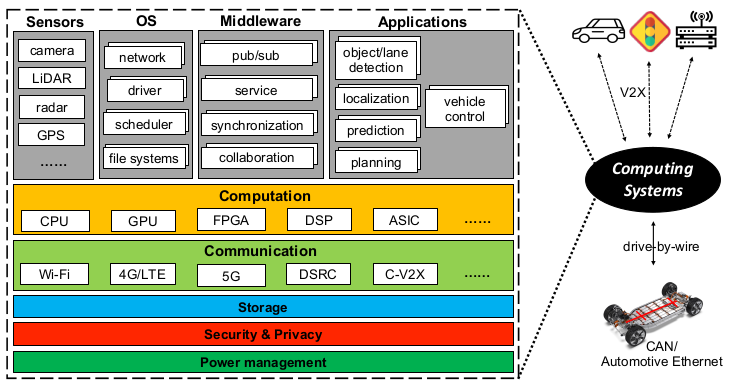
\includegraphics[width=0.65\textwidth]{figures/1_introduccion/Ejemplo_de_arquitectura_de_un_sistema_de_conduccion_autonoma.png}
	\caption{Ejemplo de arquitectura de un sistema de conducci�n auton�ma.}
	\label{fig:Ejemplo_de_arquitectura_de_un_sistema_de_conduccion_autonoma}
\end{figure}
La evoluci�n continua de estos sistemas trata de ofrecer un mayor nivel de seguridad al volante con \ac{adas}, para que en un futuro puedan ser remplazados por \ac{ads}.\\
Para analizar el avance de estos sistemas y para poder compararlos, se ha dividido seg�n su nivel de autonom�a, por lo que se tiene desde un nivel 0 a un nivel 5. El nivel 0 indica que el coche no tiene ning�n tipo de autonom�a, en el nivel 1 el vehiculo sigue siendo controlado por el conductor pero ciertas caracter�sticas de ayuda a la conducci�n son a�adidas, en el siguiente nivel el veh�culo es capaz de acelerar, frenar y hasta dirigir el veh�culo pero con el conductor siempre atento, en el nivel 3 el conductor es necesario pero no es requerimiento la atenci�n al entorno, pero debe de estar listo para tomar en control en todo momento, el nivel 4 permite un nivel de autonom�a donde el veh�culo no requiere de atenci�n pero unicamente en ciertos escenarios y el �ltimo nivel es el que habilita la conducci�n aut�noma completa \cite{automated_vehicles_for_safety}.
\begin{figure}[H]
	\centering
	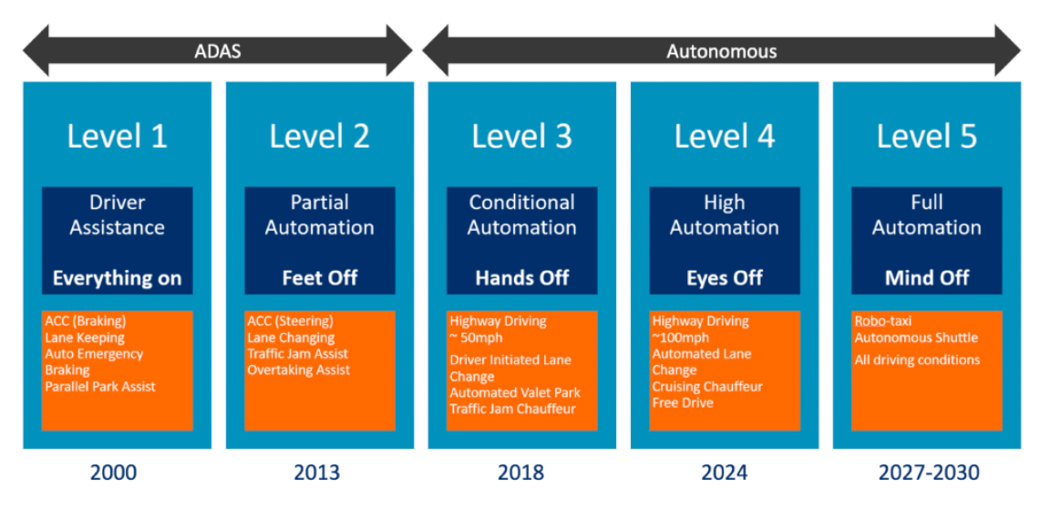
\includegraphics[width=0.8\textwidth]{figures/1_introduccion/Niveles_de_autonomia.png}
	\caption{Niveles de autonomia.}
	\label{fig:Niveles_de_autonomia}
\end{figure}
El desarrollo de este tipo de sistemas no es una tarea sencilla, m�ltiples empresas involucradas en el desarrollo de veh�culos aut�nomos pretend�an tener veh�culos en el nivel 4 de autonom�a en poco tiempo, pero como se ha visto esto no es posible, actualmente nos encontramos en el mercado con sistemas que se encuentran entre el nivel 2 y el 3, por lo que a�n queda un largo camino antes de llegar a conducci�n aut�noma completa.

\section{Sistemas de percepci�n}
\label{sec:sistemas-de-percepcion}

Los sistemas de \acs{ads}/\acs{adas} requieren de un entendimiento del entorno para poder funcionar correctamente, para ello es necesario a�adir diversos sensores a los largo del veh�culo que nos permitan obtener la mayor informaci�n del exterior posible. A partir de este conocimiento es posible la toma de decisiones y la planificaci�n, por lo que en este apartado se va a explicar de que manera se puede configurar un sistema de percepci�n, cuales son los principales sensores y que informaci�n se puede obtener de cada uno de ellos.

\subsection{Principales sensores para la percepci�n en veh�culos aut�nomos}
\label{sec:principales-sensores-para-la-percepcion-en-vehiculos-autonomos}

Para la creaci�n un sistema de percepci�n robusto es necesario el uso de diversos tipos de sensores que ofrezcan una informaci�n de relevancia de manera diferente al resto, por ello se utilizan sensores como c�maras, \acs{radar}, \acs{lidar}, sensores de ultrasonidos, \acs{gps}, \acs{gnss}, \acs{imu} etc.\\
Estos ofrecen informaci�n de localizaci�n, velocidad, distancia de objetos en el entorno, e incluso informaci�n del propio veh�culo, como su propia localizaci�n, la velocidad lineal y angular que este tiene.\\
Tambi�n es necesario tener en cuenta que no todos los sensores funcionan de la misma manera en distintos escenario por lo que en situaciones donde un sensor es incapaz de obtener buenos datos otro sensor puede suplir esta carencia, por lo que la redundancia de sensores aporta otro nivel de seguridad al veh�culo ya no solo un nivel mayor de detecci�n del entorno.

\subsubsection{C�mara}
\label{sec:camara}

Uno de los sensores m�s utilizados es la c�mara, este es el m�s extendido debido a la gran riqueza de informaci�n que ofrece del entorno. Actualmente se pueden encontrar c�maras que generen im�genes a una gran resoluci�n y a una alta tasa de \acs{fps} por un precio bastante asequible, este es uno de los sensores m�s baratos.
\begin{figure}[H]
	\centering
	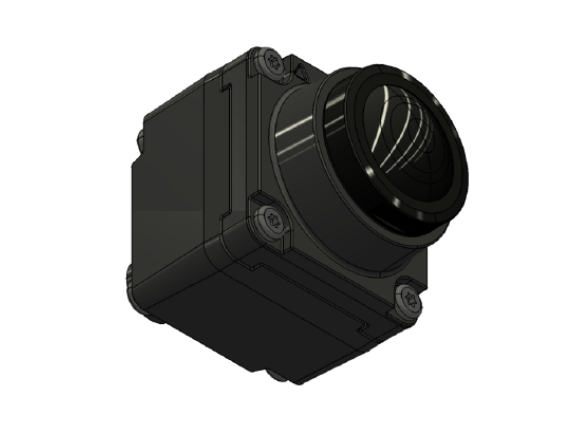
\includegraphics[width=0.4\textwidth]{figures/1_introduccion/Camara.png}
	\caption{Ejemplo de c�mara utilizado en veh�culos aut�nomos.}
	\label{fig:Ejemplo_de_camara_utilizado_en_vehiculos_autonomos}
\end{figure}
El problema de este sensor recae en el computo que es necesario para obtener informaci�n a partir de las im�genes, ya que estas no son m�s que p�xeles en escala de grises o con un sistema de colores como el RGB. Por ello no solo es necesario tener el cuenta el coste del sensor, sino que tambi�n hay que aumentar la capacidad de computo del ordenador de abordo para que pueda analizar en tiempo real las im�genes.\\
Por �ltimo es necesario conocer las limitaciones de la c�mara, esta funciona de forma correcta en situaciones de buena luminosidad y sin reflejos, por lo que en situaciones con lluvia \ref{fig:Uso_de_camara_con_lluvia}, niebla, durante la noche y otros escenarios climatol�gicos adversos, no es capaz de obtener toda la informaci�n que esta obtendr�a en situaciones m�s favorables, lo cual hace que otros sensores sean usados en estas condiciones adversas para lidiar con estar limitaciones.
\begin{figure}[H]
	\centering
	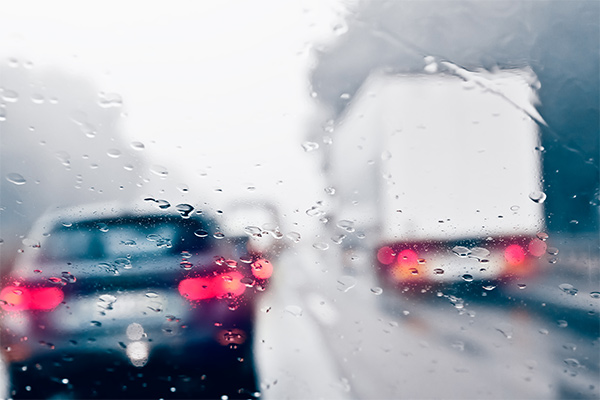
\includegraphics[width=0.5\textwidth]{figures/1_introduccion/Lluvia_camara.jpg}
	\caption{Uso de c�mara con lluvia.}
	\label{fig:Uso_de_camara_con_lluvia}
\end{figure}
A�n conociendo las desventajas de estos sensores la gran mayor�a de enfoques incluyen c�maras para la obtenci�n de los objetos del entorno tanto en 2D como en 3D, pudiendo utilizar para lo segundo un sistema de c�maras est�reo que obtienen tambi�n informaci�n de la profundidad.

\subsubsection{Radar}
\label{sec:radar}

Los \acs{radar} son utilizados en m�ltiples aplicaciones como la previsi�n meteorol�gica, la astronom�a, las comunicaciones, la navegaci�n oce�nica y la conducci�n aut�noma entre otras.\\
Este sensor emite ondas de radio, las cuales son reflejadas devuelta a este, lo cual da una informaci�n de donde se hayan los objetos en el espacio tridimensional lo cual implica la distancia a estos junto con los dos �ngulos necesarios, adem�s gracias al efecto Doppler se puede inferir la velocidad de los objetos a partir de un fen�meno que hace variar la frecuencia de la onda enviada si hay alg�n tipo de movimiento local relativo respecto del propio \acs{radar} \cite{how_self_driving_vehicles_work, doppler}.
\begin{figure}[H]
	\centering
	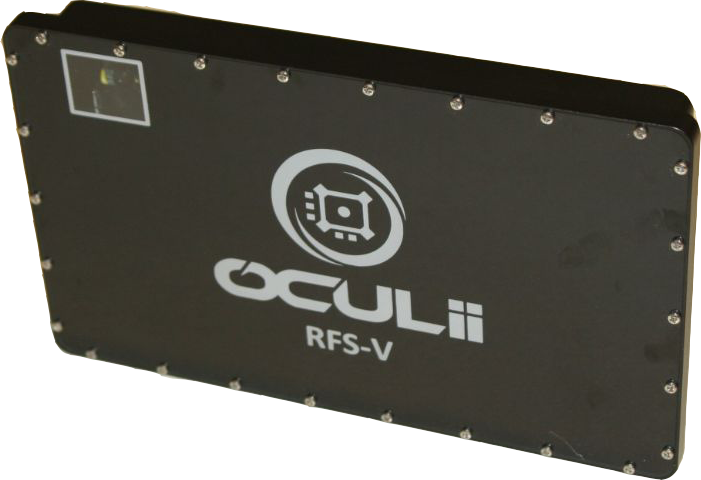
\includegraphics[width=0.4\textwidth]{figures/1_introduccion/Radar.png}
	\caption{Ejemplo de Radar utilizado en veh�culos aut�nomos.}
	\label{fig:Ejemplo_de_radar_utilizado_en_vehiculos_autonomos}
\end{figure}
Como se ha visto este sensor al contrario que la c�mara obtiene directamente informaci�n utilizable para el entendimiento del entorno de forma directa, el problema radica en la escasa cantidad de datos que provee. Aunque se obtenga informaci�n de localizaci�n 3D y de velocidad, la cantidad de la nube de puntos producida es muy peque�a, por lo que es necesario de otros sensores para obtener una informaci�n completa del entorno.\\
Por otra parte, una de las principales ventajas del \acs{radar} es que se puede utilizar en cualquier situaci�n meteorol�gica, unicamente podr�a verse afectado por lluvias muy intensas. Por lo que es un sensor muy completo y una gran adici�n para obtener informaci�n adicional de posici�n 3D y velocidad a un precio inferior a un \acs{lidar} y por ello es adoptado por gran cantidad de sistemas \acs{adas} en conjunto con sistemas de c�maras 360 alrededor del veh�culo.

\subsubsection{LiDAR}
\label{sec:lidar}

De formo similar al \acs{radar}, los sistemas \acs{lidar} basan su funcionamiento en el escaneo del entorno a partir de el env�o de l�seres y el c�lculo del tiempo desde su env�o hasta su retorno. Con esta informaci�n de distancia y el �ngulo de inclinaci�n del haz que envi� esa se�al, se construye una nube de puntos que consta de valores x, y, z de posici�n y otro valor que es el coeficiente de reflectividad del rayo de luz con el objeto incidido \cite{how_self_driving_vehicles_work}.\\
Actualmente los \acs{lidar} m�s utilizados son de 64 canales, lo cual indica que se tienen 64 l�seres funcionando al mismo tiempo lo que da una gran resoluci�n del entorno, adem�s la nube de puntos generada es de hasta 120 metros alrededor del veh�culo lo cual permite detectar objetos a una distancia considerable y saber de manera casi perfecta su distancia en un entorno tridimensional gracias a los alrededor de 2.000.000 de puntos que se generan por segundo del entorno \cite{velodyne_hdl_64}.

\begin{figure}[H]
	\centering
	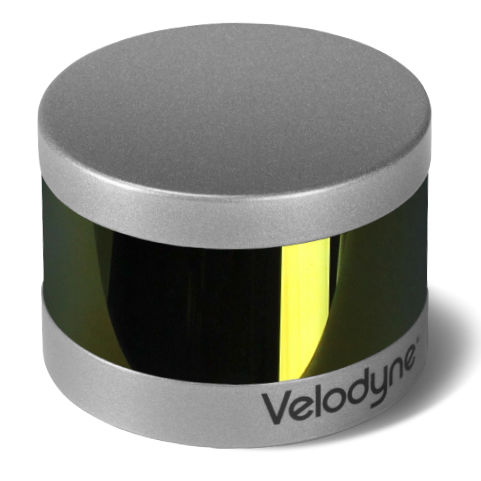
\includegraphics[width=0.3\textwidth]{figures/1_introduccion/Lidar.jpg}
	\caption{Ejemplo de LiDAR utilizado en veh�culos aut�nomos.}
	\label{fig:Ejemplo_de_lidar_utilizado_en_vehiculos_autonomos}
\end{figure}

Los sistemas \acs{lidar} tienen la ventaja de ser un sensor que aporta mucha informaci�n del entorno, pero tienen el mismo problema que las c�maras, en condiciones de lluvia, nieve, granizo o niebla, la efectividad de este sensor decae aunque se trata de minimizar ajustando la longitud de onda del l�ser utilizado \cite{lidar_adverse_weather_conditions}.\\
A�n siendo un sensor muy �til, que puede aumentar el nivel de redundancia del sistema adem�s de la seguridad, m�ltiples compa��as como Tesla tratan de evitar su uso utilizando unicamente c�maras y \acs{radar}, esto es debido a que un \acs{lidar} suele costar entre 8.000 y 100.000 d�lares si se requiere de un resoluci�n similar al estado del arte entre 16 y 128 haces \cite{computing_system_for_autonomous_driving}.

\subsection{Sistemas de detecci�n}
\label{sec:sistemas-de-deteccion}

Unicamente con un sistema de sensores no es posible la comprensi�n del entorno, tambi�n es necesario de un procesamiento de los datos, mientras que la c�mara no da ninguna informaci�n de forma directa, el \acs{lidar} y el \acs{radar} son capaces de obtener la posici�n de obst�culos alrededor del veh�culo, y adem�s el \acs{radar} es capaz de inferir la velocidad de los objetos sin necesidad de un seguimiento.\\
Principalmente en los sistemas de detecci�n para conducci�n aut�noma se trata de obtener las posiciones de los diferentes objetos de inter�s del entorno. Estas detecciones pueden ser tanto en 2D como en 3D, pero el problema radica en como obtener un rect�ngulo u ortoedro que identifique donde se encuentran dicho objetos del entorno.

\begin{figure}[H]
	\centering
	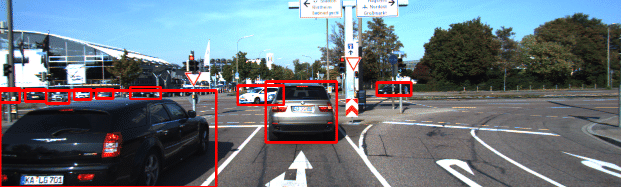
\includegraphics[width=1\textwidth]{figures/1_introduccion/Detecciones_2D.png}
	\caption{Ejemplo de detecciones 2D utilizando c�mara.}
	\label{fig:Ejemplo_de_detecciones_2d_utilizando_camara}
\end{figure}

\newpage

Una de las formas de detecci�n del entorno es a partir de c�maras, esto puede ser conseguido con un sistema de una c�mara o de un sistema multic�mara que abarque los 360 grados alrededor del coche, con esto instalado en el coche se puede generar rect�ngulos sobre las im�genes de los objetos del entorno como coches, peatones, bicicletas, motocicletas... Con esto se obtendr�a un listado de objetos detectados en 2D, lo cual es obtenible con un modelo de basado en redes neuronales como YOLO \cite{yolo} que es capaz de hacerlo en tiempo real tal y como se ve en \ref{fig:Ejemplo_de_detecciones_2d_utilizando_camara}.


\subsection{Sistemas de seguimiento}
\label{sec:sistemas-de-seguimiento}



\subsection{Fusi�n sensorial}
\label{sec:fusion-sensorial}



\section{Deep Learning}
\label{sec:deep_learning}




\chapter{Propuesta de trabajo}
\label{cha:propuesta_de_trabajo}

\begin{FraseCelebre}
  \begin{Frase}
    La educaci�n cient�fica de los j�venes es al menos tan importante, quiz� incluso m�s, que la propia investigaci�n.
  \end{Frase}
  \begin{Fuente}
    Glenn Theodore Seaborg
  \end{Fuente}
\end{FraseCelebre}

Este trabajo se encuentra dentro del proyecto Tech4AgeCars perteneciente al grupo RobeSafe. En este se pretende realizar un estudio de diferentes t�cnicas de detecci�n utilizando \acs{lidar}, tanto con m�todos cl�sicos como basados en \acl{dl} para el an�lisis en datasets reales, en el simulador \ac{carla} y en el coche del grupo RobeSafe.\par
En la arquitectura del proyecto se tiene implementado un procesamiento basado en PointPillars para una ejecuci�n en tiempo real sobre una plataforma NVIDIA Jetson AGX Xavier \cite{tfm_del_egido}, por lo que se pretende remplazar esta subtarea de detecci�n utilizando \acs{lidar}, dentro de la capa de percepci�n.\par
Con la implementaci�n de la detecci�n realizada, se pretende realizar una fusi�n sensorial entre c�mara y \acs{lidar} junto con un compa�ero del grupo RobeSafe que se encuentra realizando un TFG de detecci�n 3D utilizando c�mara \cite{tfg_miguel}.\par
Tras una fusi�n y sin la posibilidad de analizar el sistema de percepci�n a crear, se trabajar� por �ltimo en un proyecto junto con el \ac{kit} llamado \ac{ad_devkit} que tratar� de analizar un \acl{ads}, en concreto se trabajar� en el apartado de percepci�n del kit de desarrollo, todo ello esperando que este proyecto no solo sea �til para los compa�eros del proyecto sino para cualquier desarrollador que utilice el simulador \acs{carla}. 


\chapter{Sistemas cl�sicos de percepci�n con LiDAR}
\label{cha:sistemas_clasicos_de_percepcion_con_lidar}

\begin{FraseCelebre}
  \begin{Frase}
    El placer m�s noble es el j�bilo de comprender.
  \end{Frase}
  \begin{Fuente}
    Leonardo da Vinci
  \end{Fuente}
\end{FraseCelebre}

\noindent
Mientras que se tienen m�ltiples tipos de t�cnicas de percepci�n tanto cl�sicas como basadas en \acs{dl}, el uso de t�cnicas cl�sicas utilizando unicamente \acs{lidar} no abundan, por lo que se presentan las t�cnicas estudiadas e implementadas en el simulador \acs{carla} que permiten la detecci�n de los objetos del entorno.

\section{Voxelizaci�n}
\label{sec:voxelizacion}

Las nubes de puntos generadas por el \acs{lidar} pueden ser de hasta 1.300.000 puntos por segundo en un \acs{lidar} de 64 haces \cite{velodyne_hdl_64} lo que implicar�a el an�lisis de una gran cantidad de datos en tiempo real lo que puede no ser muy viable ya que se tiene una capacidad de computo limitada en un veh�culo.\par
Para ello se utiliza la voxelizaci�n, esta no solo es utilizada en sistemas de percepci�n, sino que tambi�n es utilizada en im�genes volum�tricas de �mbito m�dico, para la representaci�n del terreno o en el pipeline gr�fico de un ordenador. Esta t�cnica trata de reducir la cantidad de datos en memoria a la vez que reduce el computo al reducir la resoluci�n de la escena. Por lo que se puede entender como un proceso de discretizaci�n del entorno.

\begin{figure}[H]
	\centering
	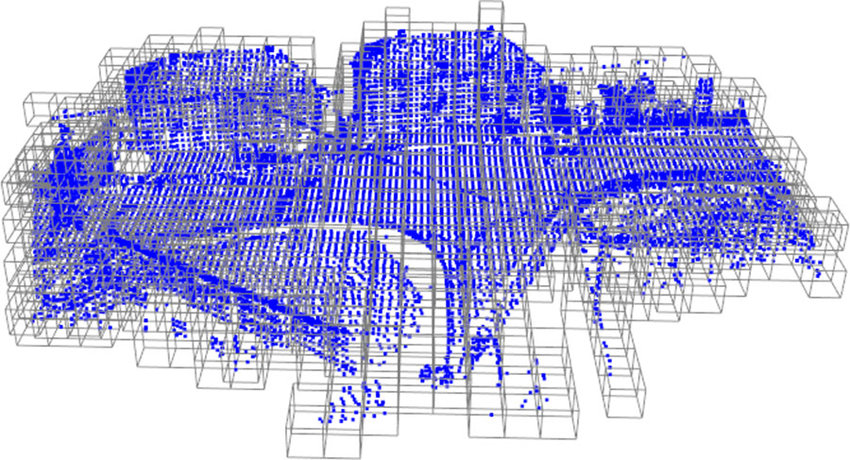
\includegraphics[width=0.6\textwidth]{figures/3_sistemas_clasicos_de_percepcion/entorno_voxelizado.png}
	\caption{Entorno 3D voxelizado.}
	\label{fig:Entorno_3d_voxelizado}
\end{figure}

\newpage

Trabajando con nubes de puntos, la voxelizaci�n sigue los siguientes pasos:
\begin{enumerate}
	\item Definici�n del tama�o del v�xel, lo que ser�a un vector tridimensional.
	\item A partir del tama�o del v�xel se divide la escena en un conjunto de ortoedros u v�xeles.
	\item Si se encuentra un punto del \ac{lidar} dentro de un v�xel este de activa
\end{enumerate}
\par
Esta t�cnica como se ver� en el cap�tulo \ref{cha:sistemas_de_percepcion_con_lidar_basados_en_deep_learning}, tambi�n se utiliza en diversos modelos basados en \acs{dl}, esto se hace para trabajar de forma similar a lo que ser�a la estructura de una imagen que se encuentra compuesta por p�xeles en vez de por v�xeles.

\section{RANSAC-3D}
\label{sec:ransac_3d}

Para la detecci�n de los objetos del entorno no es necesaria la informaci�n de los puntos que inciden en el suelo, por lo que una de las t�cnicas utilizadas para la selecci�n del plano perteneciente al suelo es \ac{ransac}-3D.\par
El algoritmo \acs{ransac} \cite{ransac} tiene una funcionalidad similar a la regresi�n linear, ambos algoritmos a partir de un conjunto de datos hayan la relaci�n lineal entre dos caracter�sticas. La creaci�n de este algoritmo ten�a como finalidad el ajuste de datos experimentales, el uso en el an�lisis de escenas y generaci�n autom�tica de mapas.

\begin{figure}[H]
	\centering
	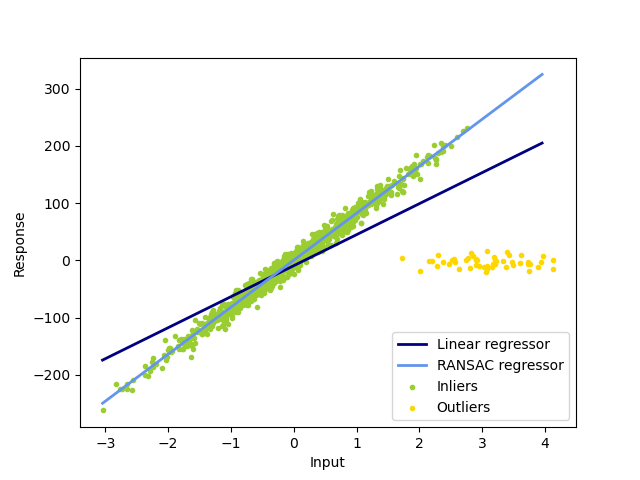
\includegraphics[width=0.7\textwidth]{figures/3_sistemas_clasicos_de_percepcion/ransac.png}
	\caption{Aplicaci�n de RANSAC para detecci�n de outliers.}
	\label{fig:Aplicacion_de_ransac_para_deteccion_de_outliers}
\end{figure}

La idea principal del algoritmo \acs{ransac} es la generaci�n de rectas a partir de 2 o m�s puntos para aceptar como la mejor recta aquella que contenga m�s puntos entre un l�mite seleccionado, y esto es repetido un n�mero arbitrario de veces. Esta recta ser� la que contenga los puntos asumidos como normales o inliers, y el resto de puntos son asumidos como an�malos o outliers. El algoritmo completo ser�a el siguiente \ref{alg:Algoritmo_ransac}.

\newpage

\begin{algorithm}[H]
	\SetAlgoLined
	\begin{algorithmic}
		\Input
		\Desc{data}{Conjunto de observaciones}
		\Desc{model}{Modelo que explica las observaciones}
		\Desc{n}{M�nimo n�mero de puntos necesarios para estimar un modelo}
		\Desc{k}{N�mero de iteraciones del algoritmo}
		\Desc{t}{Valor l�mite que indica que puntos se encuentran bien estimados}
		\Desc{d}{N�mero de puntos cercanos que asegura que el modelo sea v�lido}
		\EndInput
		\Output
		\Desc{bestFit}{Par�metros del modelo que ajustan de mejor manera a los datos}
		\EndOutput
	\end{algorithmic}
 	$iterations \leftarrow$ 0\\
 	$bestFit \leftarrow$ null\\
 	$bestError \leftarrow \infty$\\
 	
 	\While{$iterations < k$}{
  		$maybeInliers \leftarrow n$ puntos seleccionados aleatoriamente\\
  		$maybeModel \leftarrow$ modelo que se ajusta a $maybeInliers$\\
  		$alsoInliers \leftarrow$ set vac�o\\
  		\For{cada punto que no se encuentre en $maybeInliers$}{
  			\If{error de ajustar el punto a $maybeModel < t$}{
  				a�adir punto a $alsoInliers$\\
  			}
  		}
  		\If{n�mero de puntos en $alsoInliers > d$}{
  			$betterModel \leftarrow$ par�metros del modelo sobre el que han sido ajustados los puntos de $maybeInliers$ y $alsoInliers$\\
  			$thisErr \leftarrow$ medida de como de bien han sido ajustado los puntos\;
  			\If{$thisErr < bestErr$}{
  				$bestFit \leftarrow betterModel$\\
  				$bestErr \leftarrow thisErr$\\
  			}
  		}
  		$iterations \leftarrow iterations +$ 1\;
 	}
 	\caption{Algoritmo RANSAC}
 	\label{alg:Algoritmo_ransac}
\end{algorithm}

En el caso de las nubes de puntos que devuelve el \acs{lidar}, se trabaja en un entorno tridimensional, por lo que no funciona de la misma manera dicho algoritmo, se utiliza una variaci�n, \acs{ransac}-3D como se ve en \ref{fig:Aplicacion_de_ransac_3d}, que en vez de trabajar con datos en 2D se trabajan en 3D por lo que en vez de ajustar un modelo lineal se ajusta como un plano, por lo que como m�nimo se necesitan tres puntos para generar un posible modelo ya que es el m�nimo n�mero de puntos para generar un plano, el resto funciona de forma similar definiendo el l�mite de distancia, iteraciones...\par

Como se explic�, los resultados suelen ser similares a una regresi�n linear en un entorno bidimensional, pero en este caso no ser�a del todo cierto, ya que el plano que abarca m�s puntos suele ser en la mayor�a de los casos el correspondiente al suelo. Esto implica una modificaci�n de la regresi�n linear a las tres dimensiones, lo ser�a una regresi�n ajustada a un plano, esta generar�a en la mayor�a de las situaciones un plano que se encontrar�a por encima del suelo, ya que se tratar�a de minimizar una m�trica de error al plano (distancia eucl�dea, manhattan, minkowski, hamming...), por lo que los objetos de la escena conseguir�an levantar el plano para minimizar el error de este a los puntos correspondientes a los objetos.

\begin{figure}[H]
	\centering
	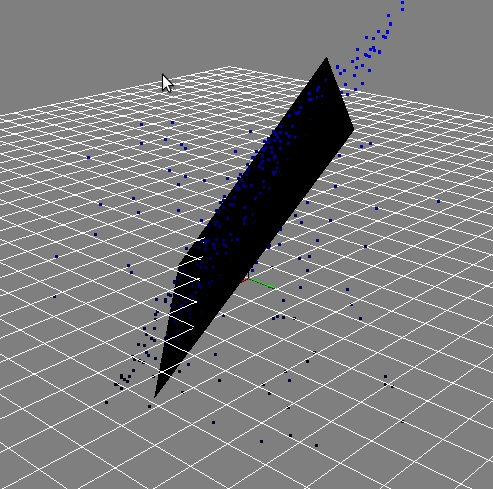
\includegraphics[width=0.35\textwidth]{figures/3_sistemas_clasicos_de_percepcion/ransac_3d.jpg}
	\caption{Aplicaci�n de RANSAC-3D.}
	\label{fig:Aplicacion_de_ransac_3d}
\end{figure}

Al tener el resto de puntos por encima del suelo, nos encontrar�a ante una situaci�n en la que el algoritmo \acs{ransac}-3D ajustar�a como inliers los puntos correspondientes al suelo y el resto se detectar�an como outliers, por lo que es este el algoritmo seleccionado al ajustarse de la mejor manera a la tarea necesitada.

\section{KD-tree}
\label{sec:kd_tree}

Tras la eliminaci�n del suelo en la nube de puntos podemos encontrarnos con que los diferentes objetos del entorno se encuentran separados, ya que el suelo era el elemento unificador de la mayor�a de puntos de la escena. Teniendo esto, es necesaria de una t�cnica que sea capaz de agrupar los puntos m�s cercanos de para que se agrupen por distancia, ya que si se hace comprobando cada punto con el resto se obtendr�a una complejidad de $O(n�)$.\par
Teniendo en cuenta el coste computacional de los algoritmos de clustering y al trabajar con tantos puntos, alrededor de 1.000.000 por segundo y sabiendo que un \acs{lidar} suele trabajar a 10 Hz, es muy recomendable aplicar una voxelizaci�n si no se aplic� previamente en la eliminaci�n de los puntos incidentes en el suelo.\par
Para el clustering, se podr�a utiliza el algoritmo \ac{knn}, pero esto producir�a cl�steres no v�lidos al encontrarse objetos con pocos v�xeles o con demasiados lo que producir�a cl�steres incompletos y otros mal formados sin no se tiene un cuenta una distancia m�xima entre v�xeles.\par
El KD-tree \cite{kd_tree} es una estructura de datos que con un eficiente uso de memoria, es capaz de hacer b�squedas en un entorno K dimensional con una complejidad media de $O(\log n)$, esto lo convierte en una gran estructura para trabajar con datos en un entorno tridimensional, como es el caso de las nubes de puntos o de v�xeles. Un KD-tree tiene una estructura similar a un �rbol binario, la eficiencia de la estructura radica en la ordenaci�n del mismo, donde en cada altura del �rbol se ordena seg�n una dimensi�n iterativamente.\par
Antes de analizar en profundidad la estructura KD-tree, es necesario comprender los �rboles binarios, tanto su uso, como su utilidad. Los �rboles binarios son una estructura de datos donde cada nodo tiene otros dos nodos hijos, referidos como hijo izquierdo e hijo derecho. La utilidad de la estructura radica en la forma en la que se pueden guardar los datos, mientras que para buscar un valor en una lista, es necesario iterar por todos ellos o hasta que se encuentre con una complejidad m�xima de $O(n)$, un KD-tree tiene una complejidad m�xima es de $O(\log_2 n)$.

\newpage

\begin{algorithm}[H]
	\SetAlgoLined
	\begin{algorithmic}
		\Input
		\Desc{tree}{�rbol binario ordenado}
		\Desc{key}{Clave del nodo buscado}
		\EndInput
		\Output
		\Desc{node}{Nodo buscado}
		\EndOutput
	\end{algorithmic}
	$node \leftarrow$ null\;
	$currentNode \leftarrow$ nodo ra�z de $tree$\\
	\While{currentNode $\neq$ null}{
		\If{clave de $currentNode = key$}{
			$node \leftarrow currentNode$\\
			\textbf{break}\;
		}
		\eIf{clave de $currentNode < key$}
		{
			$currentNode \leftarrow$ hijo derecho de $currentNode$\\
		}{
			$currentNode \leftarrow$ hijo izquierdo de $currentNode$\\
		}
	}
 	\caption{B�squeda en �rbol binario ordenado}
 	\label{alg:Busqueda_en_arbol_binario_ordenado}
\end{algorithm}

En el caso del �rbol de la figura \ref{fig:Arbol_binario_ordenado} para buscar el n�mero 7:
\begin{enumerate}
	\item Se empieza por el nodo con valor 8
	\item Al ser 7 $<$ 8 se pasa al hijo de la izquierda
	\item Como 7 $>$ 3 se salta al hijo de la derecha
	\item Teniendo el nodo con valor 6, siendo menor que 7 se coge el hijo de la derecha
	\item Por �ltimo se lleg� al nodo con valor 7 requerido
\end{enumerate}
Teniendo 9 nodos solo ha sido necesario analizar 4 nodos que la peor situaci�n con este �rbol.

\begin{figure}[H]
	\centering
	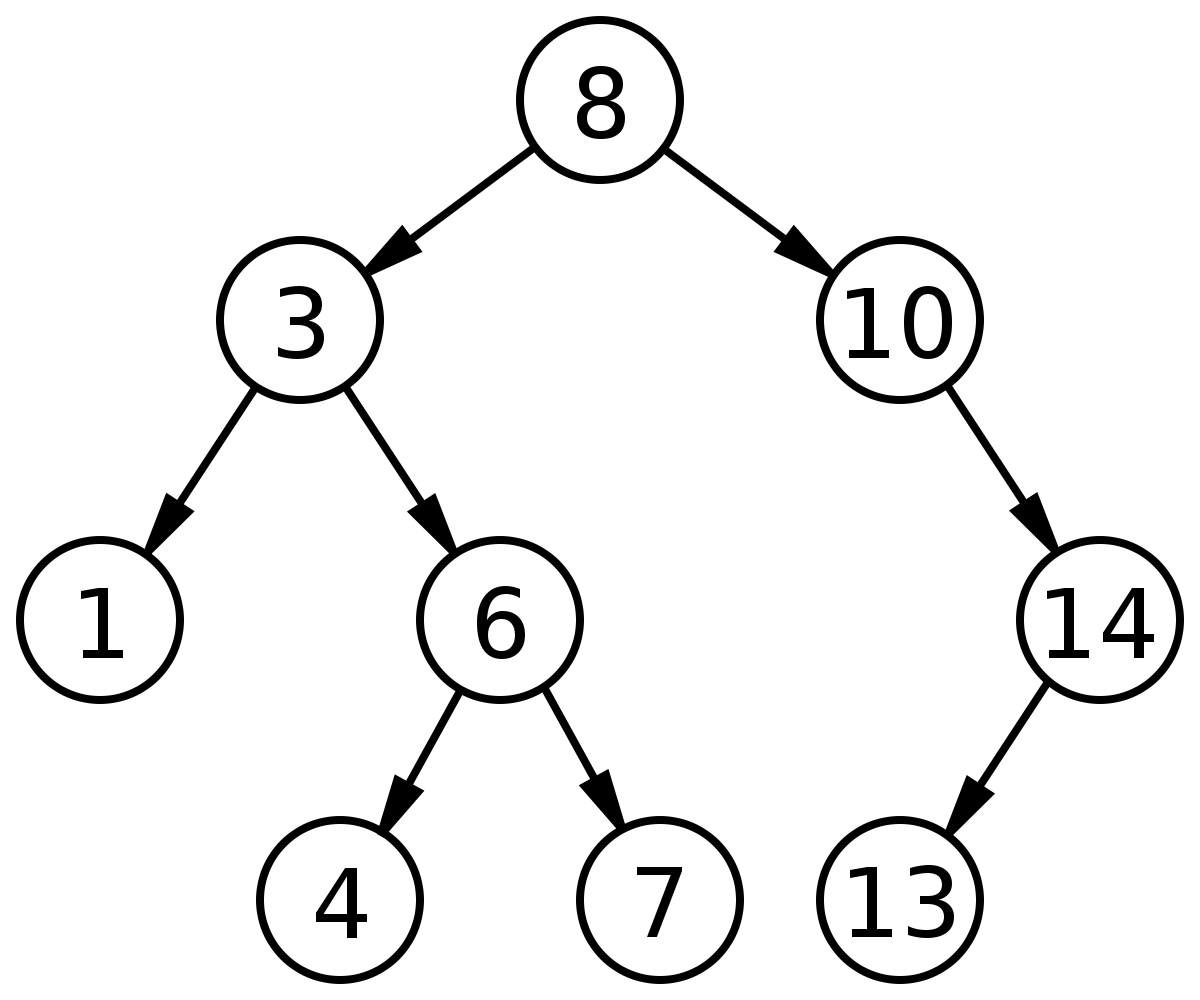
\includegraphics[width=0.35\textwidth]{figures/3_sistemas_clasicos_de_percepcion/binary_tree.png}
	\caption{�rbol binario ordenado.}
	\label{fig:Arbol_binario_ordenado}
\end{figure}

Al contrario que los �rboles binarios, un KD-tree es capaz de un n�mero K de dimensiones, por lo que hay una diferencia principal que es la rotaci�n entre la dimensi�n sobre la que se ordena en cada altura del �rbol. Esto produce que la forma de inserci�n \ref{alg:Insercion_en_KD_tree} y b�squeda sea modificada.

\newpage

\begin{algorithm}[H]
	\SetAlgoLined
	\begin{algorithmic}
		\Input
		\Desc{tree}{KD-tree}
		\Desc{node}{Nodo a introducir}
		\Desc{k}{N�mero de dimensiones del �rbol}
		\EndInput
		\Output
		\Desc{tree}{KD-tree con el nodo introducido}
		\EndOutput
	\end{algorithmic}
	$currentNode \leftarrow$ nodo ra�z de $tree$\\
	$depth \leftarrow$ 0\\
	\While{$currentNode \neq$ null}{
		$x \leftarrow depth$ mod $k$\\
		\eIf{valor de $currentNode$ en la dimensi�n $x <$ valor de $node$ en la dimensi�n $x$}
		{
			$currentNode \leftarrow$ hijo derecho de $currentNode$\\
		}{
			$currentNode \leftarrow$ hijo izquierdo de $currentNode$\\
		}
		$depth \leftarrow depth +$ 1
	}
	$currentNode \leftarrow node$
 	\caption{Inserci�n en KD-tree}
 	\label{alg:Insercion_en_KD_tree}
\end{algorithm}

Lo que produce esta forma de guardar los datos en el �rbol, es que seg�n se aumenta la profundidad en el �rbol, la regi�n de los nodos hijos es cada vez menor, lo que permite una m�s sencilla agrupaci�n y estudio de los datos por regiones en un entorno K dimensional. Como se ve en la figura \ref{fig:Espacio_bidimensional_dividido_por_un_kd_tree} el espaci� bidimensional va siendo dividido por regiones, esto es gracias a que cada nodo divide en dos el espacio sobre el que se encuentran sus hijos, lo cual es una perfecta manera de agrupar los puntos en cl�steres utilizando esta estructura, tal y como se detalla en el algoritmo \ref{alg:Cluster_por_distancia_en_KD_tree}

\begin{figure}[H]
	\begin{minipage}{0.48\textwidth}
		\centering
		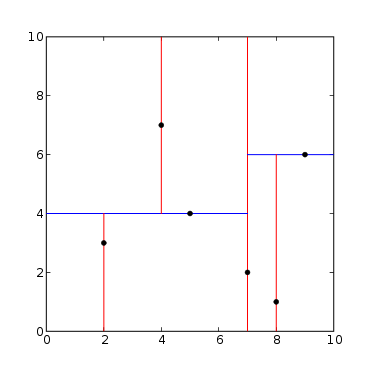
\includegraphics[width=0.9\linewidth]{figures/3_sistemas_clasicos_de_percepcion/kd_space.png}
		\caption{Espacio bidimensional dividido por un KD-tree.}
		\label{fig:Espacio_bidimensional_dividido_por_un_kd_tree}
	\end{minipage}\hfill
	\begin{minipage}{0.48\textwidth}
		\centering
		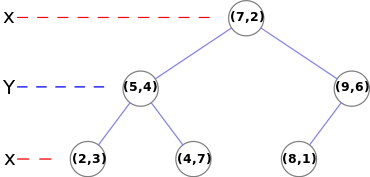
\includegraphics[width=1\linewidth]{figures/3_sistemas_clasicos_de_percepcion/kd_tree.png}
		\caption{Estructura de un KD-tree de dos dimensiones.}
		\label{fig:Estructura_de_un_kd_tree_de_dos_dimensiones}
	\end{minipage}
\end{figure}

\newpage

\begin{algorithm}[H]
	\SetAlgoLined
	\begin{algorithmic}
		\Input
		\Desc{points}{Nube de puntos del LiDAR}
		\Desc{id\_node}{Id del punto sobre el que se va a comenzar el cl�ster}
		\Desc{node}{Nodo sobre el que buscar un cl�ster}
		\Desc{processed}{Vector de booleanos de tama�o igual al n�mero de puntos}
		\Desc{tree}{KD-tree}
		\Desc{distance}{Distancia m�xima a los puntos del cl�ster}
		\Desc{k}{N�mero de dimensiones del �rbol}
		\EndInput
		\Output
		\Desc{cluster}{Conjunto de los puntos perteneciente al cl�ster}
		\EndOutput
	\end{algorithmic}
	\SetKwFunction{SearchNodes}{searchNodes}
	\SetKwFunction{Search}{search}
	\SetKwFunction{Proximity}{proximity}
	\SetKwProg{Fn}{Function}{:}{}
	\Fn{\Proximity{$points$, $id\_node$, $node$, $cluster$, $processed$, $tree$, $distance$, $k$}}{
		$processed$[$id\_node$] $\leftarrow$ true\\
		a�adir a $cluster$ $points$[$id\_node$]\\
		$indexList \leftarrow$ \Search{$points$[$id\_node$], $tree$, $distance$, $k$} 
		\For{$index$ en $indexList$}{
			\If{$processed$[$index$] $=$ false}{
				\Proximity{$points$, $index$, $cluster$, $processed$, $tree$, $distance$, $k$}
			}
		}
	}
	
	\Fn{\Search{$node$, $tree$, $distance$, $k$}}{
		$indexList \leftarrow$ lista vac�a\\
		\SearchNodes{$node$, $tree$, 0, $distance$, $indexList$, $k$}\\
		\Return $indexList$\\
	}
	
	\Fn{\SearchNodes{$node$, $tree$, $distance$, $depth$, $indexList$, $k$}}{
		\If{$tree \neq$ null}{
			\If{distancia entre el nodo ra�z de $tree$ y $node < distance$}{
				a�adir �ndice del nodo ra�z de $tree$ a $indexList$
			}
		}
		$x \leftarrow depth$ mod $k$\\
		\If{valor de $node$ en la dimensi�n $x - distance <$ valor del nodo ra�z de $tree$ en la dimensi�n $x$}{
			\SearchNodes{$node$, �rbol izquierdo de $tree$, $depth + $1, $distance$, $indexList$, $k$}\\
		}
		\If{valor de $node$ en la dimensi�n $x + distance >$ valor del nodo ra�z de $tree$ en la dimensi�n $x$}{
			\SearchNodes{$node$, �rbol derecho de $tree$, $depth + $1, $distance$, $indexList$, $k$}\\
		}
	}
 	\caption{Cluster por distancia en KD-tree}
 	\label{alg:Cluster_por_distancia_en_KD_tree}
\end{algorithm}

Gracias a la estructura KD-tree, se puede reducir la cantidad de nodos o puntos analizados, ya que cada punto no tiene que ser estudiado con el resto sino que solo se estudian los puntos que est�n una regi�n cercana dentro del radio m�ximo de distancia definido. Lo que produce una complejidad de $O(n)$ para la construcci�n de la estructura m�s la complejidad $O(n * \log n)$ de la funci�n de clustering por distancia, por lo que en total se tendr�a una mejora de complejidad de $O(n�)$ a $O(n * \log n)$.\par
La eficiencia de esta estructura en ciertas tareas, ha producido que a pesar de ser una t�cnica del a�o 1975, se siga estudiando para su utilizaci�n junto a \acs{knn} \cite{knn_kd_tree}, aumentar su rendimiento con datos preordenados \cite{kd_tree_presorted} o la paralelizaci�n de su construcci�n y t�cnicas como \acs{knn} \cite{kd_tree_gpu}.

\newpage

\section{Filtrado previo y posterior a la detecci�n}
\label{sec:filtrado_previo_y_posterior_a_la_deteccion}

Tras la obtenci�n de las detecciones por parte de los diversos algoritmos cl�sicos podemos encontrarnos ante diferentes problemas con dichas detecciones.\par
Estas pueden generar cl�steres con pocos o demasiados puntos, lo que puede resultar en cl�steres incorrectos. Aquellos con pocos puntos pueden identificar objetos lejanos u objetos que no son necesarios para el entendimiento de la escena, por otra parte, aquellas detecciones con muchos puntos pueden identificar camiones, veh�culos de construcci�n o simplemente objetos muy cercanos, pero tambi�n es muy normal que las construcciones sean detectadas por lo que hay que filtrar tanto por un n�mero m�ximo como m�nimo de puntos para obtener mejores detecciones.\par
Otra pr�ctica para el filtrado, es el ajuste a unos tama�os prefijados en todas las dimensiones, lo cual elimine aquellos objetos que no son similares a los veh�culos que se desean detectar.\par
Estas t�cnicas de filtrado no solo se pueden utilizar tras la obtenci�n de las detecciones, sino que la nube de puntos obtenida del \acs{lidar} es posible filtrarla, para que as� solo se trabaje con una regi�n de inter�s, ya que a partir de cierta distancia las detecciones no van a ser muy precisas, para ello se puede filtrar por distancia al veh�culo. Adem�s, un filtrado que permita trabajar unicamente con la parte delantera y trasera del coche, aporta una reducci�n en el computo de los algoritmos, a la vez que se reducen las falsas detecciones.


\chapter{Sistemas de percepci�n con LiDAR basados en Deep Learning}
\label{cha:sistemas_de_percepcion_con_lidar_basados_en_deep_learning}

\begin{FraseCelebre}
  \begin{Frase}
    Si no conozco una cosa, la investigar�.
  \end{Frase}
  \begin{Fuente}
    Louis Pasteur
  \end{Fuente}
\end{FraseCelebre}

\noindent
Los sistemas de percepci�n pertenecientes al estado del arte o \ac{sota} se encuentran basados en Deep Learning, esto no es diferente en los sistemas de percepci�n basados en \acs{lidar}, por lo que en este cap�tulo se presentan los datasets disponibles para el entrenamiento y evaluaci�n de los modelos, las diferentes arquitecturas \acs{sota} para detecci�n con \acs{lidar} y la herramienta utilizada para la evaluaci�n, entrenamiento y pruebas realizadas sobre los modelos.

\section{Principales datasets}
\label{sec:principales_datasets}

Para el desarrollo de un modelo de percepci�n basado en Deep Learning, es siempre necesario un conjunto de datos anotados o dataset sobre el que un modelo pueda aprender a partir de estos. En los �ltimos a�os muchas compa��as han lanzado datasets para poder entrenar y validar sus modelos, adem�s de que se muchos de estos datasets han sido publicados Open-Source para fomentar el desarrollo de nuevas t�cnicas.\par
Entre los datasets para conducci�n aut�noma encontramos: A2D2 Dataset \cite{a2d2_dataset}, Argoverse Dataset \cite{argoverse_dataset}, CityScapes Dataset \cite{cityscapes_dataset}, KITTI Vision Benchmark Suite \cite{kitti_dataset}, Level 5 Open Data \cite{level_5_dataset}, nuScenes Dataset \cite{nuscenes_dataset} o Waymo Open Dataset \cite{waymo_dataset} entre otros.\par
En este apartado se van a presentar tres de los datasets m�s importante en la industria del autom�vil, como son KITTI, nuScenes y Waymo dataset.

\subsection{KITTI}
\label{sec:kitti}

La suite de evaluaci�n de KITTI \cite{kitti_dataset} es un sistema de evaluaci�n para veh�culos aut�nomos, donde se ha desarrollado una plataforma de referencia para tareas de visi�n estereosc�pica, flujo �ptico, odometr�a visual/\acs{slam} y detecci�n de objetos 3D.\par
Este dataset fue presentado en 2012 en conjunto por el \acs{kit} y el \acs{ttic}, iniciando lo que a�os despu�s despertar�a un inter�s en la creaci�n de datasets Open-Source para sistemas \acs{adas}/\acs{ads}. Al ser el primer dataset con reconocimiento internacional, fij� las bases de lo que ser�a el futuro de los sistemas de evaluaci�n, adem�s que ha sido desde su salida uno de los sistemas de evaluaci�n m�s estandarizados en el desarrollo de t�cnicas de conducci�n aut�noma, como se puede ver en sus m�s de 7.000 citas.

\begin{figure}[H]
	\begin{forest}
	for tree={
    	font=\ttfamily,
        grow'=0,
        child anchor=west,
        parent anchor=south,
        anchor=west,
        calign=first,
        inner xsep=7pt,
        edge path={
        	\noexpand\path [draw, \forestoption{edge}]
          	(!u.south west) +(7.5pt,0) |- (.child anchor) pic {folder} \forestoption{edge label};
        },
        % style for your file node 
        file/.style={edge path={\noexpand\path [draw, \forestoption{edge}]
          	(!u.south west) +(7.5pt,0) |- (.child anchor) \forestoption{edge label};},
        	inner xsep=2pt,font=\small\ttfamily
                     },
        before typesetting nodes={
        	if n=1
            {insert before={[,phantom]}}
            {}
        },
        fit=band,
        before computing xy={l=15pt},
	}  
    [KITTI Dataset
      [2011\_09\_26
        [2011\_09\_26\_drive\_0001\_sync
          [image\_00
            [data
              [0000000000.txt,file
              ]
              [0000000???.txt,file
              ]
            ]
            [timestamps.txt,file
            ]
          ]
          [image\_01
            [...,file
    	  	]
          ]
          [image\_02
            [...,file
    	  	]
          ]
          [image\_03
            [...,file
    	  	]
          ]
          [oxts
            [data
              [0000000000.txt,file
              ]
              [0000000???.txt,file
              ]
            ]
            [dataformat.txt,file
            ]
            [timestamps.txt,file
            ]
          ]
          [velodyne\_points
            [data
              [0000000000.bin,file
              ]
              [0000000???.bin,file
              ]
            ]
            [timestamps.txt,file
            ]
            [timestamps\_end.txt,file
            ]
            [timestamps\_start.txt,file
            ]
          ]
    	]
    	[2011\_09\_26\_drive\_0???\_sync
    	  [...,file
    	  ]
    	]
    	[...,file
    	]
      ]
      [20??\_??\_??
      	[...,file
      	]
      ]
      [...,file
      ]
    ]
	\end{forest}
\caption{Estructura del dataset de KITTI.}
\label{for:Estructura_del_dataset_kitti}
\end{figure}

\newpage

El sistema de percepci�n del veh�culo utilizado para la grabaci�n de los datos se encuentra compuesto de:
\begin{itemize}
	\item 2 sistemas de c�maras est�reo de una resoluci�n de 1240 x 376 p�xeles.
	\item 1 \acs{lidar} Velodyne HDL-64E capaz de generar m�s de un mill�n de puntos por segundo gracias a sus 64 haces l�ser.
	\item 1 sistema de localizaci�n \acs{sota} compuesto por \acs{gps}, \acs{gnss}, \acs{imu} y correcci�n de se�ales \acs{rtk}.
\end{itemize}

\begin{figure}[H]
	\begin{minipage}{0.48\textwidth}
		\centering
		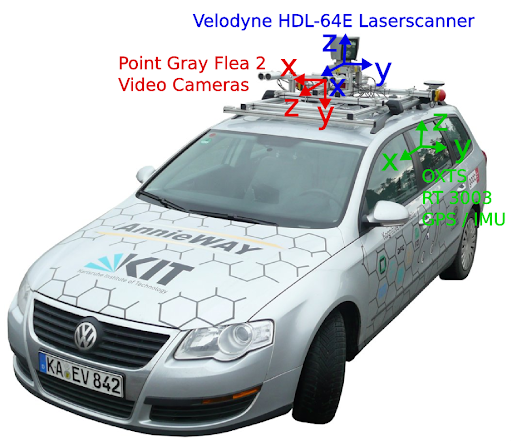
\includegraphics[width=1\linewidth]{figures/4_sistemas_de_percepcion_con_lidar_basados_en_deep_learning/kittis_car.png}
		\caption{Veh�culo utilizado en KITTI.}
		\label{fig:Vehiculo_utilizado_en_kitti}
	\end{minipage}\hfill
	\begin{minipage}{0.48\textwidth}
		\centering
		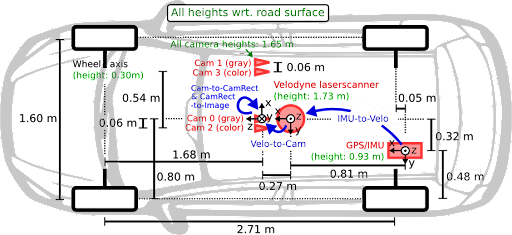
\includegraphics[width=1\linewidth]{figures/4_sistemas_de_percepcion_con_lidar_basados_en_deep_learning/kittis_car_measures.png}
		\caption{Medidas del veh�culo utilizado en KITTI}
		\label{fig:Medidas_del_vehiculo_utilizado_en_kiti}
	\end{minipage}
\end{figure}

La estructura del dataset es tal y como se muestra en la figura \ref{for:Estructura_del_dataset_kitti}. Dentro de este los datos se dividen seg�n el d�a de grabaci�n y la escena, y dentro de cada escena se tienen las im�genes de la c�mara est�reo monocrom�tica (image\_00, image\_01) y RGB (image\_02, image\_03), informaci�n de todo el sistema de locaci�n del veh�culo (oxts) y las nubes de puntos provenientes del \acs{lidar} (velodyne\_points).\par
En 2020 tras el �xito que ha sido este dataset se anuncia y se abre al uso KITTI-360 \cite{kitti_360_dataset} la evoluci�n del dataset KITTI, el cual trae mejoras a�adiendo dos c�maras de ojo de pez para una obtenci�n de visi�n 2D en todos los �ngulos del veh�culo, y una unidad l�ser adicional SICK. Adem�s se incluyen en el dataset bounding boxes 3D de todo el entorno, anotaciones de instancia a partir de la informaci�n del \acs{lidar} y anotaciones de confianza sobre el v�deo tomado por las c�maras, entre otras.

\subsubsection{An�lisis de la estructura del GT y las PCLs de KITTI}
\label{sec:analisis_de_la_estructura_del_gt_y_las_pcls_de_kitti}

Al estar basado este trabajo en la detecci�n utilizando \acs{lidar}, se estudia la forma en la que se guardan los datos de las nubes de puntos junto con la representaci�n del ground truth, para ello se analiza tanto la carpeta de velodyne\_points como el archivo tracklets.xml.\par
Para el trabajo con bounding boxes 3D, es posible utilizar unicamente el kit de detecciones 3D que contiene un conjunto de txt con la informaci�n de los objetos por cada barrido. La informaci�n de estos archivos contiene la informaci�n de: tipo, truncado, ocluido, bounding box 2D, dimensiones y localizaci�n, toda esta informaci�n se encuentra de la misma manera en el archivo tracklets.xml, pero la informaci�n de rotaci�n se encuentra divida en un �ngulo alpha y otro rotation\_y, en vez de rotaci�n por cada uno de los tres ejes, de estos se estudiar� m�s en profundidad en el cap�tulo \ref{cha:ad_devkit}.\par
Se utiliza el archivo tracklets.xml ya define el ground truth de la escena pero no por cada barrido del \acs{lidar}, sino que se guarda por cada escenario, lo que se traduce en un estructura se puede utilizar tanto para detecci�n como para seguimiento de los objetos, todo ello como un archivo con formato \acs{xml}.\par
Se ha decido crear un programa que lea la nube de puntos indicada y que marque en un entorno 3D donde se encuentran los objetos de la escena. Esto podr�a ser realizado mediante el devkit que KITTI ofrece, pero este se encuentra unicamente de forma oficial en Matlab, por lo que como los modelos de Deep Learning a utilizar se encuentran utilizando Pytorch, se deber�an de analizar los datos utilizando Python.\par
La figura \ref{for:Estructura_del_archivo_tracket_labels_xml} muestra la estructura de los principales atributos del archivo tracklet\_labels.xml analizado, en este encontramos el n�mero de los diferentes objetos del escenario, tras esto se analiza cada objeto a trav�s de los diferentes barridos, mostrando primero las caracter�sticas de los objetos que se mantienen en el tiempo, como las dimensiones o el tipo de objeto y tras esto se guarda la informaci�n de posici�n, rotaci�n, etc.

\begin{figure}[H]
	\begin{forest}
	for tree={
    	font=\ttfamily,
        grow'=0,
        child anchor=west,
        parent anchor=south,
        anchor=west,
        calign=first,
        inner xsep=7pt,
        edge path={
        	\noexpand\path [draw, \forestoption{edge}]
          	(!u.south west) +(7.5pt,0) |- (.child anchor) pic {folder} \forestoption{edge label};
        },
        % style for your file node 
        file/.style={edge path={\noexpand\path [draw, \forestoption{edge}]
          	(!u.south west) +(7.5pt,0) |- (.child anchor) \forestoption{edge label};},
        	inner xsep=2pt,font=\small\ttfamily
                     },
        before typesetting nodes={
        	if n=1
            {insert before={[,phantom]}}
            {}
        },
        fit=band,
        before computing xy={l=15pt},
	}  
    [tracklet\_labels.xml
      [tracklets,file
        [count,file
        ]
        [item,file
          [objectType,file
          ]
          [h,file
          ]
          [w,file
          ]
          [l,file
          ]
          [first\_frame,file
          ]
          [poses,file
            [count,file
            ]
            [item,file
              [tx,file
              ]
              [ty,file
              ]
              [tz,file
              ]
              [rx,file
              ]
              [ry,file
              ]
              [rz,file
              ]
              [state,file
              ]
              [occlusion,file
              ]
              [truncation,file
              ]
            ]
            [...,file]
          ]
        ]
        [...,file
        ]
      ]
    ]
	\end{forest}
\caption{Estructura del archivo tracklet\_labels.xml.}
\label{for:Estructura_del_archivo_tracket_labels_xml}
\end{figure}

Tras dicho an�lisis, utilizando la librer�a MayaVi para la visualizaci�n del entorno 3D, NumPy para las transformaciones en el espacio y Beautiful Soup para la lectura del \acs{xml}, se visualizan m�ltiples escenas del dataset.\par
Cabe destacar que como KITTI est� realizado para que la parte de percepci�n se trabaje principalmente con la c�maras frontales del veh�culo, a�n teniendo informaci�n por los laterales y la parte trasera gracias al \acs{lidar}, esta no se tiene en cuenta en el ground truth, raz�n por la que en la imagen \ref{fig:Visualizacion_de_una_nube_de_puntos_de_kitti_junto_con_su_ground_truth} los veh�culos de la parte trasera no se muestra.

\begin{figure}[H]
	\centering
	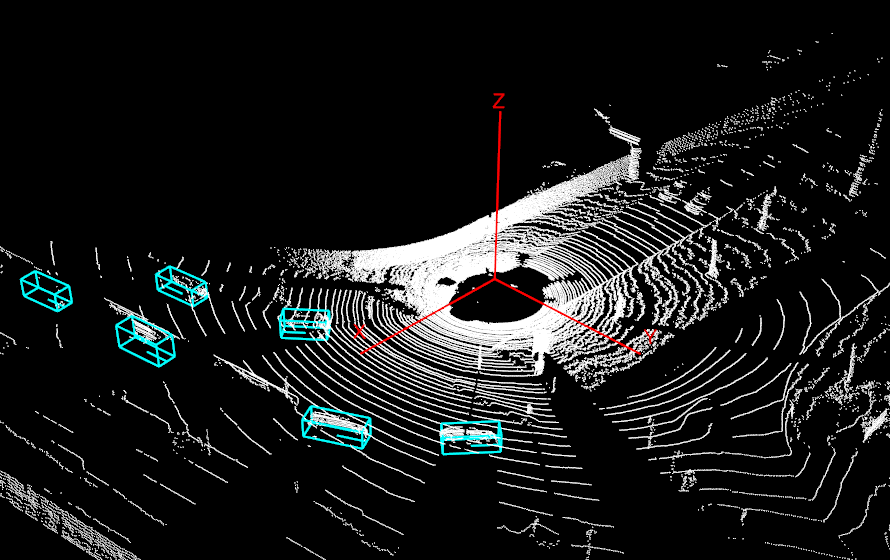
\includegraphics[width=0.55\textwidth]{figures/4_sistemas_de_percepcion_con_lidar_basados_en_deep_learning/display_kitti_example.png}
	\caption{Visualizaci�n de una nube de puntos de KITTI junto con su ground truth.}	\label{fig:Visualizacion_de_una_nube_de_puntos_de_kitti_junto_con_su_ground_truth}
\end{figure}

Todo el c�digo utilizado para la visualizaci�n de los objetos junto con unos escenarios de ejemplo son accesibles en: \url{https://github.com/Javier-DlaP/Display_kitti_pcl_annotations} 

\subsection{Waymo}
\label{sec:waymo}

Waymo Open Dataset \cite{waymo_dataset} es el dataset liberado de forma Open-Source por parte de Waymo y Google para la aceleraci�n del desarrollo de tecnolog�as de conducci�n aut�noma.\par
La propuesta de este dataset es la oferta de un gran n�mero de anotaciones de alta calidad tanto 2D como 3D,  que adem�s contienen informaci�n de seguimiento. Se han utilizado m�ltiples ciudades para sus escenario grabados, como son: San Francisco, Mountain View, Los Angeles, Detroit, Seattle y Phoenix. Adem�s se trabaja con multitud de entornos y condiciones ambientales como son: construcciones, atardeceres, noches, d�as lluviosos, etc.

\begin{figure}[H]
	\centering
	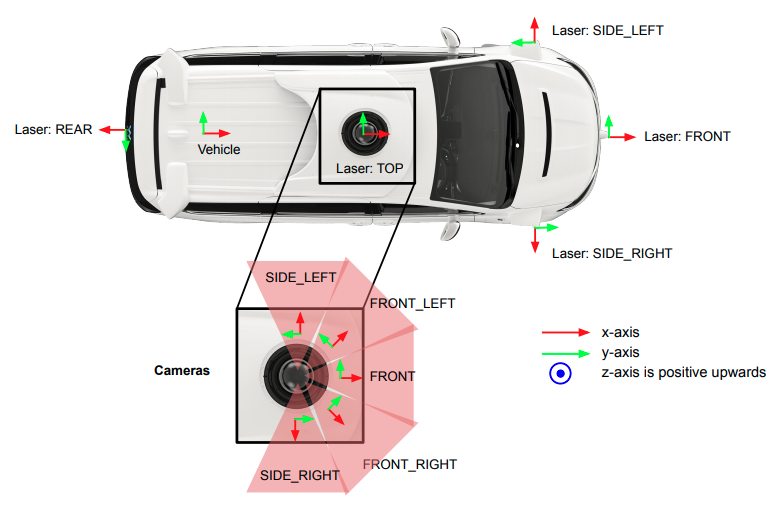
\includegraphics[width=0.6\textwidth]{figures/4_sistemas_de_percepcion_con_lidar_basados_en_deep_learning/waymos_car.png}
	\caption{Veh�culo utilizado en Waymo.}
	\label{fig:Veh�culo_utilizado_en_waymo}
\end{figure}

\newpage

Actualmente el dataset ofrece 1.950 escenas \cite{waymo_web_page} que fueron aumentadas de las 1150 escenas en la salida de la primera revisi�n del paper, de 20 segundos cada una,
con informaci�n recogida a 10 Hz proveniente de los sensores, lo que implican
390.000 frames. Toda esta informaci�n es recabada de:
\begin{itemize}
	\item 1 \acs{lidar} de medio alcance.
	\item 4 \acs{lidar} de corto alcance.
	\item 5 c�maras alrededor del veh�culo.
\end{itemize}
Como se ve en la figura \ref{fig:Veh�culo_utilizado_en_waymo}, el acercamiento de la compa��a entorno a la construcci�n del veh�culo no utiliza \acs{radar}, depende unicamente de c�maras y \acs{lidar} para el apartado de percepci�n. Por lo que no se puede trabajar con \acs{radar} en el dataset, adem�s de que no se tiene informaci�n de ning�n sistema de localizaci�n, ya que dicho dataset se encuentra especializado en tareas de percepci�n y seguimiento de los objetos de la escena.\par
Es importante tener en cuenta que en este dataset, la nube de puntos procedente del \acs{lidar} no utiliza un sistema de coordenadas cartesiano, sino un sistema de coordenadas esf�rico, donde las coordenadas (x, y, z) son reemplazadas por (distancia, azimuth, inclinaci�n).

\begin{center}
$distancia = \sqrt{x�+y�+z�}$\\[10pt]
$azimuth = \atantwo(y, x)$\\[10pt]
$inclinaci�n = \atantwo(z, \sqrt{x�+y�})$
\end{center}

Mientras que en otros datasets se tienen multitud de clases, muchas de ellas indistinguibles unas de otras, Waymo utiliza unicamente 4 tipos de objetos diferentes. En las 11,8 millones de bounding boxes 2D se encuentran veh�culos, peatones y ciclistas, mientras que en las 12,6 millones de bounding boxes 3D se a�aden adem�s la detecci�n y seguimiento de se�ales.

\begin{figure}[H]
	\centering
	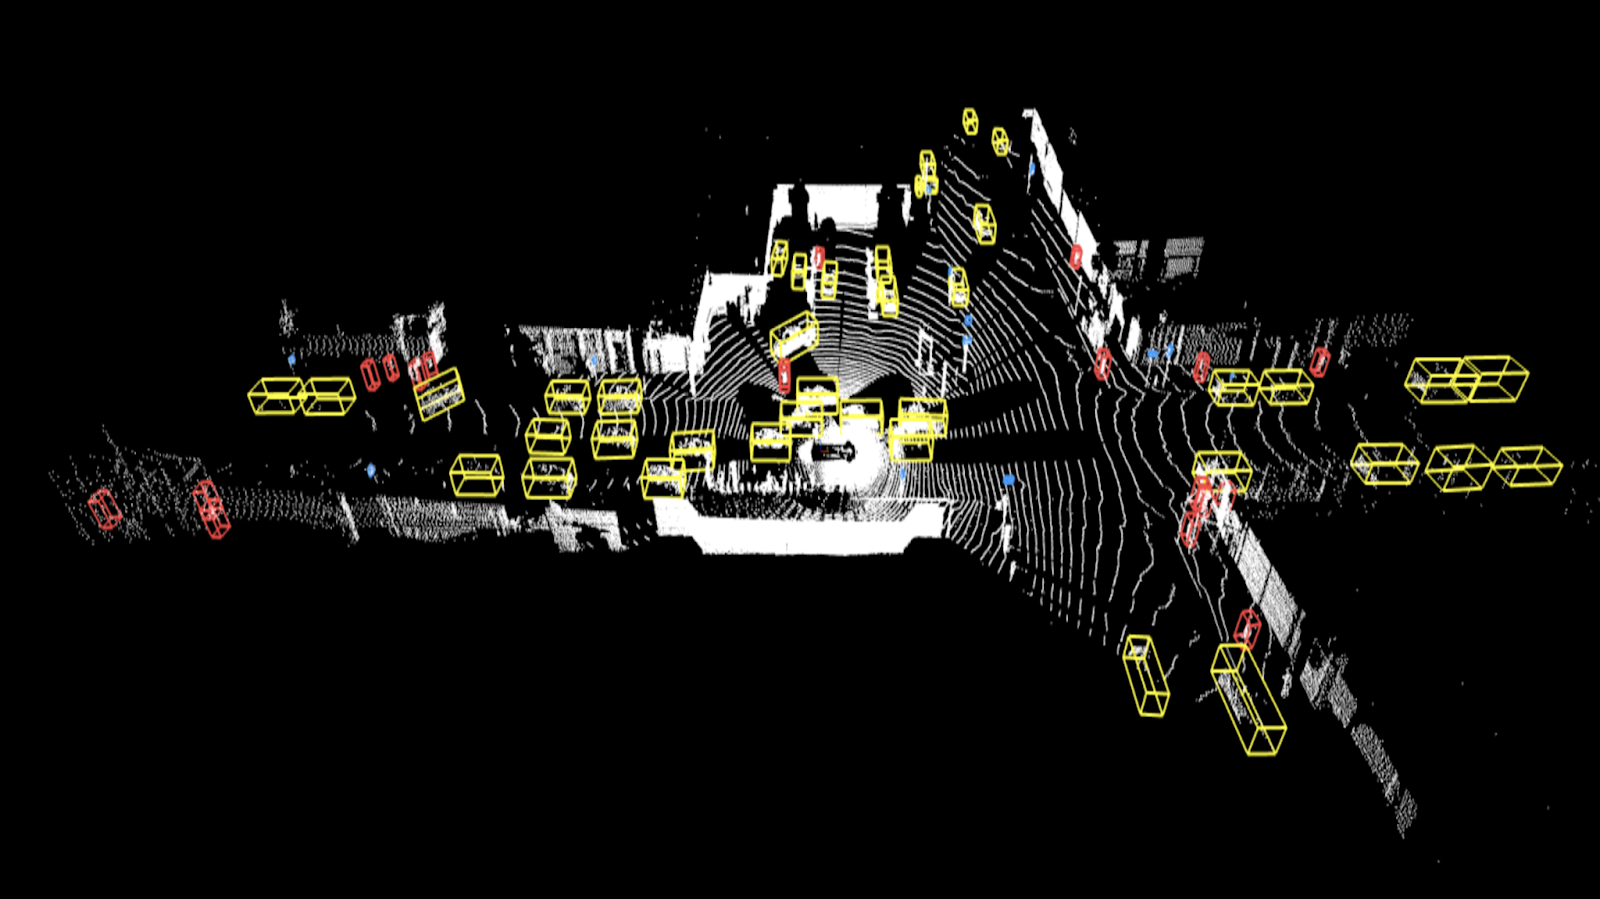
\includegraphics[width=0.6\textwidth]{figures/4_sistemas_de_percepcion_con_lidar_basados_en_deep_learning/classes_waymo.png}
	\caption{Nube de puntos con las diferentes clases del dataset de Waymo.}
	\label{fig:Nube_de_puntos_con_las_diferentes_clases_del dataset_de_waymo}
\end{figure}

En la figura \ref{fig:Nube_de_puntos_con_las_diferentes_clases_del dataset_de_waymo} encontramos las diferentes clases a detectar y seguir en el dataset, teniendo en amarillo los coches, rojo los peatones, azul las se�ales y rosa los ciclistas.\par
Waymo ofrece un dataset muy completo si solo se desea trabajar con tareas de percepci�n, compitiendo cara a cara con los datasets m�s importantes como son KITTI, nuScenes y Argoverse, teniendo adem�s uno de los sistemas de evaluaci�n para tareas de percepci�n orientadas a veh�culos aut�nomos, m�s grandes y con m�s anotaciones que se pueden encontrar de forma Open-Source.

\newpage

\subsection{nuScenes}
\label{sec:nuscenes}

NuScenes Dataset \cite{nuscenes_dataset} se presenta como una mejora a al dataset KITTI lanzado en 2012. Esta mejora no solo radica en la calidad de los datos sino en el n�mero de diferentes situaciones disponibles, de la misma manera que Waymo, ofreciendo situaciones nocturnas y d�as lluviosos.\par
En comparaci�n con otros datasets, se incluye un set m�s completo de sensores como son:
\begin{itemize}
	\item Sistema de 6 c�maras 360� con una resoluci�n de 1600 x 900.
	\item \acs{lidar} de 32 haces con una frecuencia de 20 Hz, capaz de generar hasta 1,4 millones de puntos por segundo.
	\item Sistema de 5 \acs{radar} con una distancia m�xima de 250 metros y una frecuencia de 13 Hz.
	\item Sistema de localizaci�n compuesto por \acs{gps}, \acs{imu}, \acs{ahrs} y un sistema de posicionamiento \acs{rtk}.
\end{itemize}

\begin{figure}[H]
	\centering
	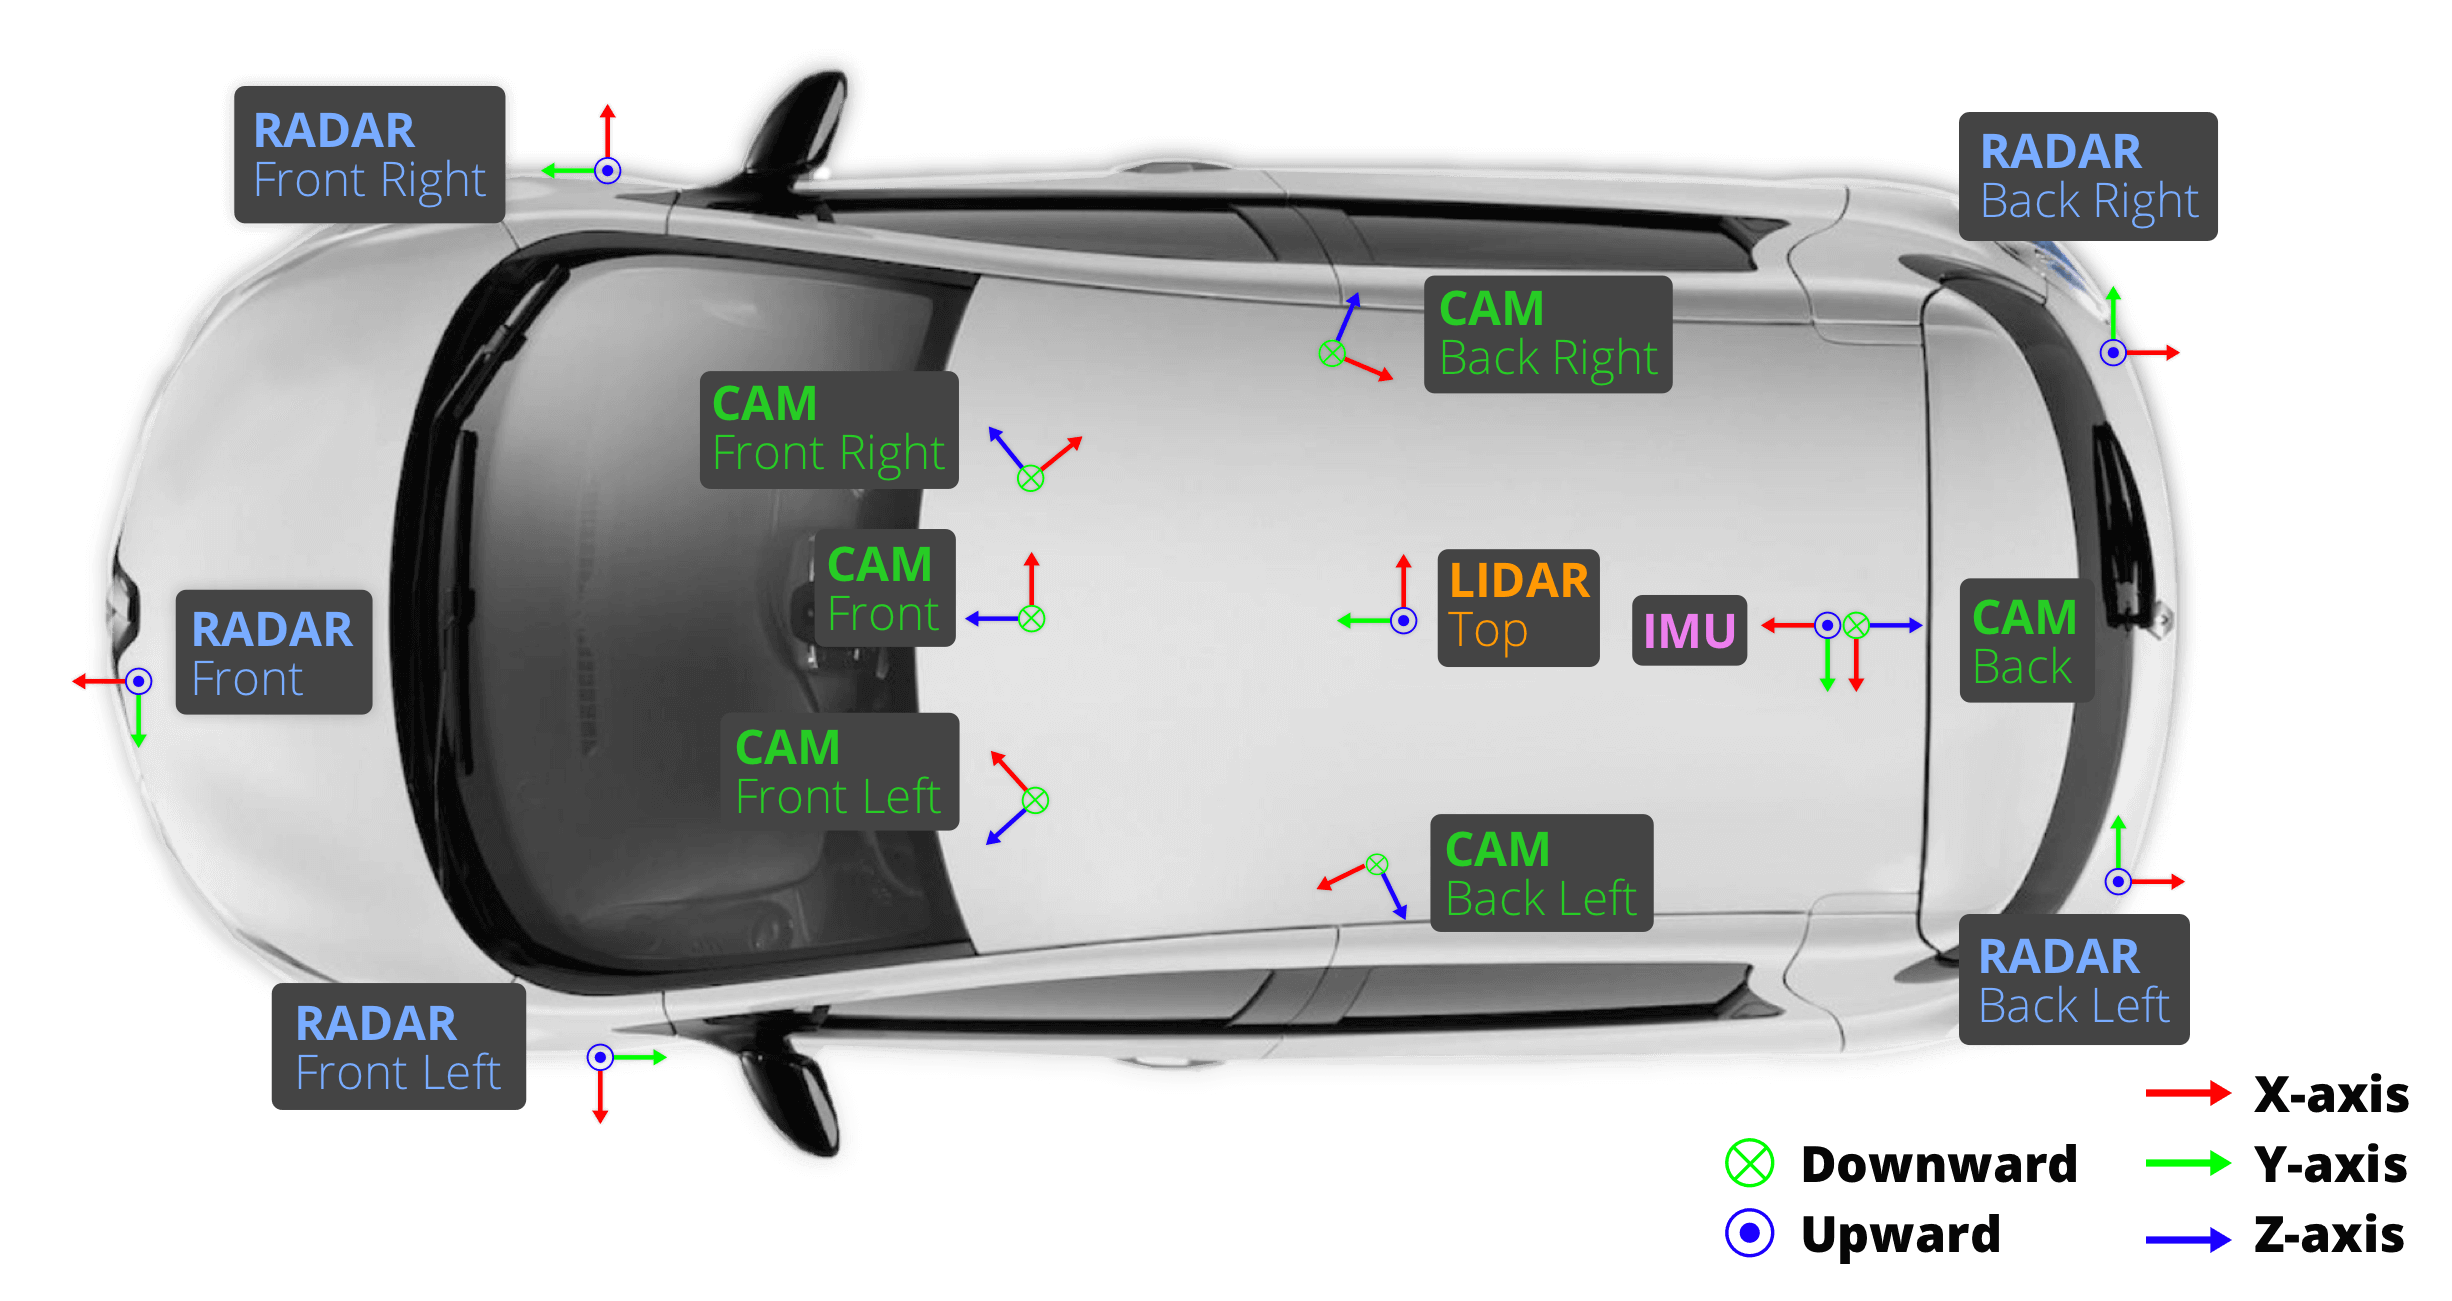
\includegraphics[width=0.6\textwidth]{figures/4_sistemas_de_percepcion_con_lidar_basados_en_deep_learning/nuscenes_car.png}
	\caption{Veh�culo utilizado en el dataset de nuScenes.}
	\label{fig:Vehiculo_utilizado_en_el_dataset_de_nuscenes}
\end{figure}

NuScenes tiene 23 clases diferentes a detectar, entre ellas se encuentran como en el resto de datasets: coches, ciclistas, peatones, etc. Pero en este se encuentran adem�s animales, diferenciaci�n por el tipo de los peatones, como ser�an polic�as o personas en silla de ruedas, adem�s de barreras entre otras. Esto permite agrupar las clases para detectar unicamente las m�s simples o servir como un sistema de evaluaci�n con toda la informaci�n necesaria para la implementaci�n en un sistema \acs{ads}.\par
El sistema de evaluaci�n de nuScenes permite evaluaci�n de m�ltiples sistemas a diferentes niveles. Las diferentes tareas a evaluar son:
\begin{itemize}
	\item Detecci�n de objetos 3D (10 tipos de objetos diferentes) utilizando c�mara, \acs{lidar}, \acs{radar} y la informaci�n de los mapas.
	\item Seguimiento de objetos 3D (7 tipos de objetos diferentes) utilizando c�mara, \acs{lidar}, \acs{radar} y la informaci�n de los mapas.
	\item Predicci�n del movimiento y de la posici�n de los objetos.
	\item Segmentaci�n de la nube de puntos del \acs{lidar} a nivel de punto.
\end{itemize}
El dataset completo de nuScenes ocupa medio terabyte, esto es debido a la cantidad de informaci�n que este tiene, la cual es encuentra dividida en: mapas, informaci�n de los sensores en los frames que se tienen anotaciones, informaci�n de los sensores sin anotaciones y una carpeta v1.0-trainval que contiene todos los archivos json que relacionan todo el dataset adem�s del ground truth \ref{for:Estructura_del_dataset_nuscenes}.

\begin{figure}[H]
	\begin{forest}
	for tree={
    	font=\ttfamily,
        grow'=0,
        child anchor=west,
        parent anchor=south,
        anchor=west,
        calign=first,
        inner xsep=7pt,
        edge path={
        	\noexpand\path [draw, \forestoption{edge}]
          	(!u.south west) +(7.5pt,0) |- (.child anchor) pic {folder} \forestoption{edge label};
        },
        % style for your file node 
        file/.style={edge path={\noexpand\path [draw, \forestoption{edge}]
          	(!u.south west) +(7.5pt,0) |- (.child anchor) \forestoption{edge label};},
        	inner xsep=2pt,font=\small\ttfamily
                     },
        before typesetting nodes={
        	if n=1
            {insert before={[,phantom]}}
            {}
        },
        fit=band,
        before computing xy={l=15pt},
	}  
    [nuScenes Dataset
        [v1.0-trainval
          [maps
          ]
          [samples
          	[CAM\_BACK
          	]
          	[CAM\_BACK\_LEFT
          	]
          	[CAM\_BACK\_RIGHT
          	]
          	[CAM\_FRONT
          	]
          	[CAM\_FRONT\_LEFT
          	]
          	[CAM\_FRONT\_RIGHT
          	]
          	[LIDAR\_TOP
          	]
          	[RADAR\_BACK\_LEFT
          	]
          	[RADAR\_BACK\_RIGHT
          	]
          	[RADAR\_FRONT
          	]
          	[RADAR\_FRONT\_LEFT
          	]
          	[RADAR\_FRONT\_RIGHT
          	]
          ]
          [sweeps
          	[CAM\_BACK
          	]
          	[CAM\_BACK\_LEFT
          	]
          	[CAM\_BACK\_RIGHT
          	]
          	[CAM\_FRONT
          	]
          	[CAM\_FRONT\_LEFT
          	]
          	[CAM\_FRONT\_RIGHT
          	]
          	[LIDAR\_TOP
          	]
          	[RADAR\_BACK\_LEFT
          	]
          	[RADAR\_BACK\_RIGHT
          	]
          	[RADAR\_FRONT
          	]
          	[RADAR\_FRONT\_LEFT
          	]
          	[RADAR\_FRONT\_RIGHT
          	]
          ]
          [v1.0-trainval
          ]
        ]
    ]
	\end{forest}
\caption{Estructura del dataset nuScenes.}
\label{for:Estructura_del_dataset_nuscenes}
\end{figure}

Dicha estructura es para el uso de todos los sensores del dataset y los mapas, pero en el caso de que se requiera unicamente de las c�maras, nuScenes ofrece nuImages, este es el dataset de nuScenes reducido, que adem�s cambia la estructura interna de este.

\begin{figure}[H]
	\begin{minipage}{0.48\textwidth}
		\centering
		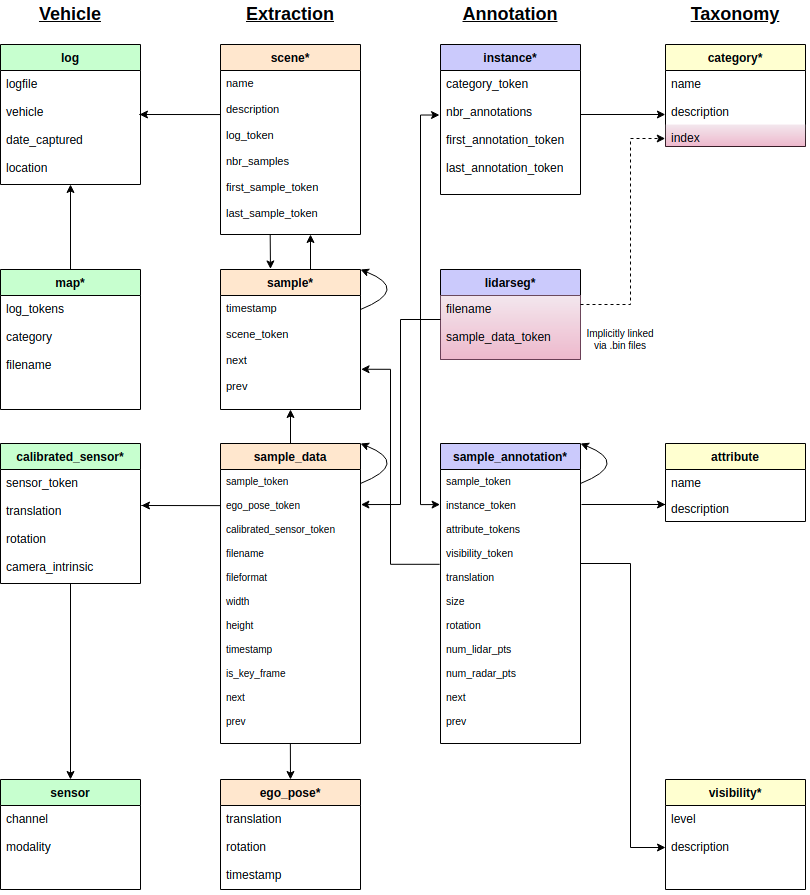
\includegraphics[width=1\linewidth]{figures/4_sistemas_de_percepcion_con_lidar_basados_en_deep_learning/nuscenes_schema.png}
		\caption{Esquema de nuScenes.}
		\label{fig:Esquema_de_nuscenes}
	\end{minipage}\hfill
	\begin{minipage}{0.48\textwidth}
		\centering
		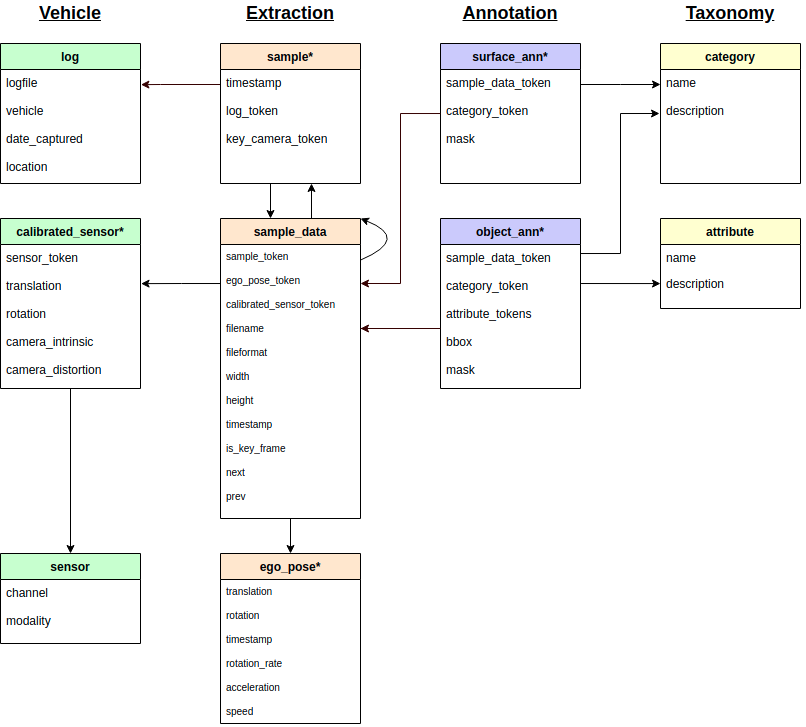
\includegraphics[width=1\linewidth]{figures/4_sistemas_de_percepcion_con_lidar_basados_en_deep_learning/nuimages_schema.png}
		\caption{Esquema de nuImages}
		\label{fig:Esquema_de_nuimages}
	\end{minipage}
\end{figure}

Las estructuras de estas versiones del dataset, no son sencillas de trabajar con los datos directamente, por lo que nuScenes ha desarrollado un devkit con el que sea m�s sencillo de trabajar con ambas estructuras tal y como se explicar� en el siguiente apartado.

\subsubsection{NuScenes devkit}
\label{sec:nuscenes_devkit}

Promover el uso de un dataset es importante en la medida que sino se tienen caracter�sticas nuevas en este o es dif�cil de utilizar, este no destacar� y desaparecer� entre la cantidad de datasets que se encuentran hoy en d�a. Para ello, nuScenes desarrolla y lanza de forma Open-Source nuScenes devkit.\par
NuScenes devkit, ofrece un uso muy simplificado del dataset de nuScenes y nuImages. Ambos datasets incorporan a partir de json una estructura similar a la de una base de datos relacional en la que a partir de claves primarias, externas e �ndices se consigue tener un conjunto de datos normalizado, para as� minimizar al m�ximo la redundancia de datos.\par
Al ofrecer una gran cantidad de datos no solo de los sensores sino de la escenas, configuraciones de calibraci�n, visibilidad, categor�as, etc. Se ha estructurado en diferentes archivos json para no tener que repetir datos por cada imagen o nube de puntos. El devkit ha sido programado para su uso en Python 3 y los tutoriales para aprender a utilizar dicho devkit se encuentran en Jupyter Notebooks, aunque tambi�n se recomienda su uso en Google Colab.\par
Para el aprendizaje del devkit de nuScenes se descarga la versi�n mini del dataset, el cual tiene la misma estructura que el dataset completo. Junto con Jupyter se estudia todo el dataset siguiendo los diferentes tutoriales que ofrece. Tras trabajar con la herramienta y acostumbrase al uso de los tokens que relacionan los diferentes archivos json, es muy sencillo obtener toda la obtener los datos requeridos.\par
A partir del devkit es muy sencillo realizar tareas como filtrado de clases, agrupaciones, transformaciones mundo a c�mara, seguimiento de objetos individualizado, etc. De esta manera se ahorra mucho tiempo en la construcci�n de complejas funciones ya  que se encuentran insertadas en el kit de desarrollo, adem�s de que permite ver de forma anal�tica el comportamiento del dataset.

\begin{figure}[H]
	\centering
	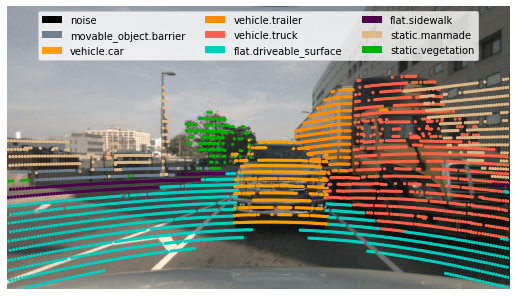
\includegraphics[width=0.6\textwidth]{figures/4_sistemas_de_percepcion_con_lidar_basados_en_deep_learning/lidar_segmentation.png}
	\caption{Transformaci�n mundo a imagen de la nube de puntos segmentada en el devkit de nuScenes.}
	\label{fig:Transformacion_mundo_a_imagen_de_la_nube_de_puntos_segmentada_en_el_devkit_de_nuscenes}
\end{figure}

Con c�digo tan simple como el siguiente \ref{cod:Obtencion_de_una_nube_de_puntos_segmentada_sobre_una_imagen_utilizando_nuscenes_devkit} es muy f�cil obtener la imagen de una c�mara con la nube de puntos segmentada tras realizar una transformaci�n de mundo a c�mara tal y como se ve en la figura \ref{fig:Transformacion_mundo_a_imagen_de_la_nube_de_puntos_segmentada_en_el_devkit_de_nuscenes}. Dichas transformaciones como se ver� en el cap�tulo \ref{cha:ad_devkit} no es algo inmediato, por lo es necesario cierto conocimiento del funcionamiento de las c�maras y de transformaciones geom�tricas.

\begin{codefloat}
\begin{lstlisting}[language=Python]
from nuscenes import NuScenes

nusc = NuScenes(version='v1.0-mini',
                dataroot='/home/javier/nuScenes-dataset-mini-v1.0',
                verbose=True)
my_sample = nusc.sample[87]

nusc.render_pointcloud_in_image(my_sample['token'],
                                pointsensor_channel='LIDAR_TOP',
                                camera_channel='CAM_BACK',
                                render_intensity=False,
                                show_lidarseg=True,
                                filter_lidarseg_labels=[22, 23],
                                show_lidarseg_legend=True)

\end{lstlisting}
\caption{Obtenci�n de una nube de puntos segmentada sobre una imagen utilizando nuScenes devkit}
\label{cod:Obtencion_de_una_nube_de_puntos_segmentada_sobre_una_imagen_utilizando_nuscenes_devkit}
\end{codefloat}

\subsection{Comparativa entre los diferentes datasets}
\label{sec:comparativa_entre_los_diferentes_datasets}

Tras el estudio y an�lisis de los datasets de KITTI, Waymo y nuScenes se obtiene un conocimiento de las arquitecturas hardware utilizadas en el estado de arte del campo de los datasets de conducci�n aut�noma, adem�s de los sistemas de evaluaci�n utilizados.\par
Mientras que KITTI fue el primero en desarrollo en un dataset para conducci�n aut�noma, hasta hace muy poco estaba casi estandarizado en la comparativa de modelos  aplicables a conducci�n aut�noma. Waymo y nuScenes aparecieron a�os m�s tarde con una apuesta clara en el uso de m�s sensores, adem�s del estudio de los 360� del entorno y no solo de la parte frontal del veh�culo como realiza KITTI.\par
En la parte del hardware, se ha visto que el acercamiento por parte de KITTI de tener 4 c�maras es un enfoque equivocado para un coche real, ya que se necesita tener un rango de visi�n mayor en el sistema de c�maras. Por parte del uso del \acs{lidar}, se encuentra con que KITTI solo se usa la parte frontal de la nube de puntos, mientras que Waymo y nuScenes utilizan toda la nube de puntos para generar las detecciones. Entre estos dos datasets encontramos diferencias en la cantidad de \acs{lidar} utilizados, ya que mientras nuScenes utiliza solo uno, Waymo utiliza cinco, lo cual obtiene mucha m�s informaci�n del entorno y una nube de puntos m�s densa, pero aumenta en mayor medida el precio de un prototipo con estas caracter�sticas. El \acs{radar} es un sensor desaparecido tanto en KITTI como en Waymo pero que se encuentra en nuScenes ofreciendo una nube de puntos de 360� que es capaz de inferir la velocidad de los objetos pero con una menor cantidad de puntos que una proveniente del \acs{lidar}.

\begin{table}[H]
	\begin{center}
		\begin{tabular}{|c|c|c|c|c|c|c|c|c|} 
		\hline
		Dataset & A�o & Situaciones & Horas & C�maras & LiDAR & RADAR & Clases & Devkit\\ 
		\hline\hline
		KITTI & 2012 & 22 & 1,5 & 4 & 1 & 0 & 8 & S� \\ 
		\hline
		Waymo & 2019 & 1000 & 5,5 & 5 & 5 & 0 & 4 & No \\
		\hline
		nuScenes & 2019 & 1150 & 5,5 & 6 & 1 & 5 & 23 & S� \\
		\hline
		\end{tabular}
		\caption{Comparativa entre los principales datasets.}
		\label{tab:Comparativa_entre_los_principales_datasets}
	\end{center}
\end{table}

En relaci�n a la cantidad de situaciones y de datos Waymo y nuScenes se encuentran en un estado similar con una gran cantidad de datos del entorno, mientras que KITTI se queda m�s atr�s debido a la longevidad del dataset.\par
Unicamente KITTI y nuScenes cuentan con un devkit, este es utilizado para uso m�s simplificado del dataset, aunque en el caso de nuScenes es casi requerido su uso. El problema de KITTI en este aspecto es el uso de Matlab para el uso del devkit ya que la mayor�a de la comunidad investigadora no utiliza este lenguaje para la creaci�n de los modelos de detecci�n, aunque se pueden encontrar de forma no oficial, repositorios Open-Source que ofrecen variantes del devkit de KITTI en otros lenguajes.\par
En conclusi�n, KITTI ha sido una gran base para la generaci�n de la siguiente generaci�n de datasets, aunque para sistemas de percepci�n algo m�s complejos se puede quedar corto, lo cual se ha ido mejorando con el tiempo y por esto mismo se est� desarrollando KITII-360. Por otra parte, Waymo y nuScenes ofrecen un dataset m�s completo, aunque nuScenes ofrece informaci�n de un sensor m�s y contiene la informaci�n de los mapas. Debido a esto se ha decidido estudiar m�s en profundidad y trabajar con los dataset de KITTI y nuScenes.

\section{Estado del arte en detecci�n utilizando LiDAR}
\label{sec:estado_del_arte_en_deteccion_utilizando_lidar}

Las t�cnicas basadas en Deep Learning que hacen uso de \acs{cnn} llevan unos a�os siendo \acs{sota} en el campo de la detecci�n utilizando unicamente \acs{lidar}. En este apartado se van a estudiar los principales modelos de detecci�n en este campo que hacen uso de estas t�cnicas.

\subsection{SECOND}
\label{sec:second}

SECOND (Sparsely Embedded CONvolutional Detector) \cite{second} se publica en 2018 para superar los modelos de detecci�n 3D, utilizando unicamente \acs{lidar}. Para ello propone una arquitectura basada en tres componentes principales: extractor de caracter�sticas a nivel de v�xel, \ac{cnn} dispersa y \ac{rpn}. Precedido todo ello de una fase de preprocesamiento de la nube de puntos y con una obtenci�n a posteriori de las salidas del modelo.

\begin{figure}[H]
	\centering
	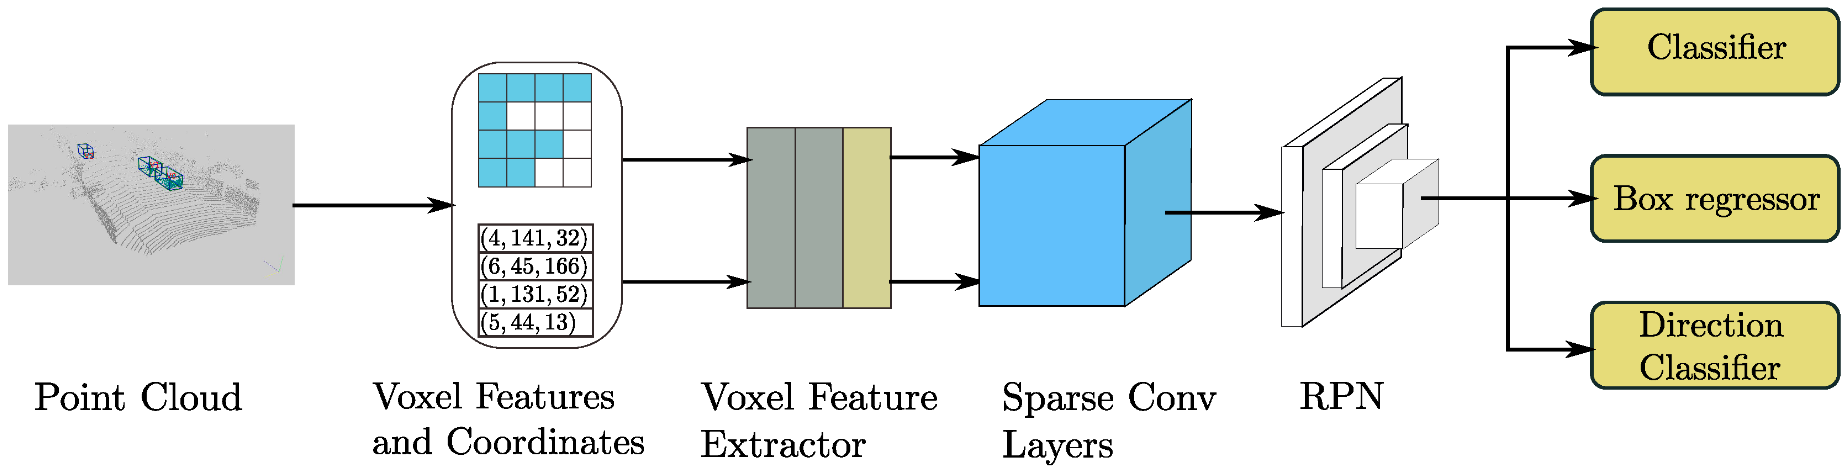
\includegraphics[width=1\textwidth]{figures/4_sistemas_de_percepcion_con_lidar_basados_en_deep_learning/second.png}
	\caption{Arquitectura propuesta del detector SECOND.}
	\label{fig:Arquitectura_propuesta_del_detector_second}
\end{figure}

Las diferentes fases del modelo que son utilizadas son las siguientes:
\begin{enumerate}
\item Preprocesamiento de la nube de puntos\par
Se comienza con la voxelizaci�n de la nube de puntos haciendo uso de una tabla hash, para su r�pido acceso en memoria. Al tener que definir un tama�o de v�xel fijo en funci�n de lo que se desee detectar, se ajusta el tama�o de la \acs{roi}, ya que como se trabajar con KITTI solo se utiliza la parte frontal del \acs{lidar}. Para la detecci�n de coches y otros veh�culos se usa [-3, 1] x [-40, 40] x [0, 70.4] m y para el modelo m�s peque�o se utiliza [-3, 1] x [-32, 32] x [0, 52.8] m para no tener que computar tantos v�xeles como el modelo completo. Todas las versiones del modelo utilizan un tama�o de v�xel fijo de [0.4, 0.2, 0.2] m y por cada uno de ellos se guarda un m�ximo de 35 puntos.
\item Extractor de caracter�sticas a nivel de v�xel\par
Se utiliza una capa \ac{vfe} tal como se presenta en el detector VoxelNet \cite{voxelnet} para extraer las caracter�sticas. Para ello se utiliza una \ac{fcn} compuesta de capas \acs{fc}, una capa que aplica batch nomalization y una \ac{relu} de salida para extraer las caracter�sticas a nivel de punto y se aplica max pooling para la obtenci�n de las caracter�sticas a nivel de v�xel.
\item Extractor convolucional disperso\par
El uso de Sparse Convolutional Networks  ofrece una mejora en rendimiento de al no computar una salida si no hay una entrada dada. Al trabajar con una nube de puntos voxelizada se consigue un mejora en el rendimiento al no utilizar aquellos v�xeles que no contienen ning�n punto. Para poder aplicar este tipo de redes es necesario hallar que indices del kernel van a ser utilizados, y para ello se necesita un algoritmo que contenga las reglas para indicar que parte del kernel es utilizado.

\begin{figure}[H]
	\centering
	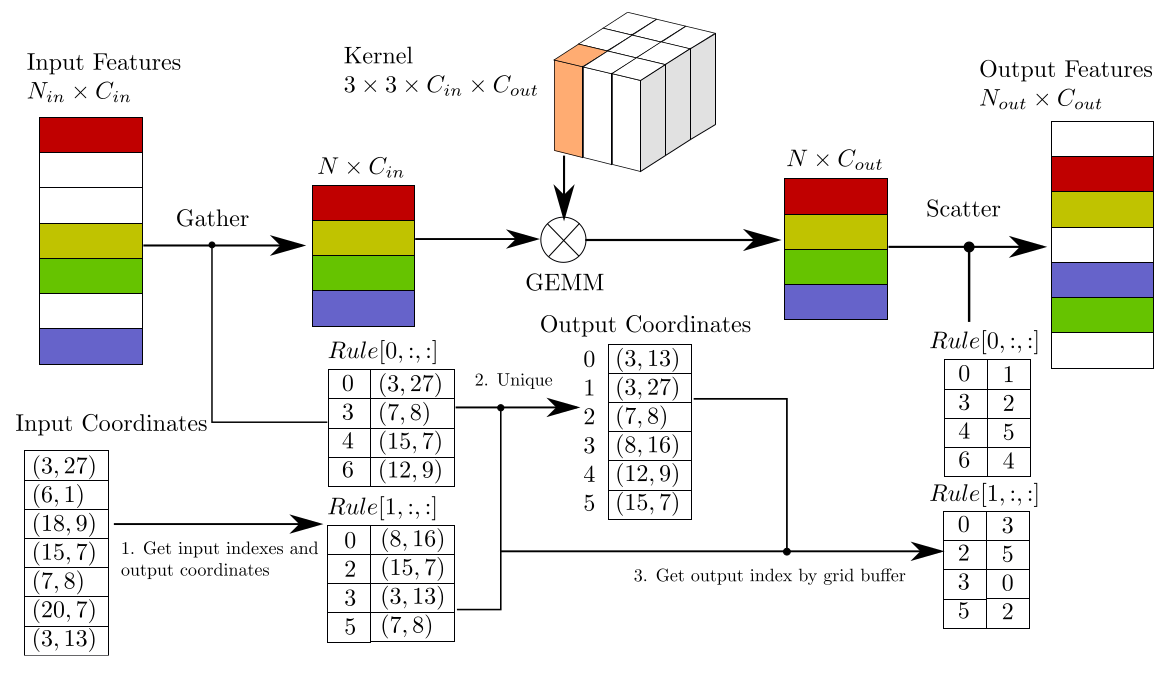
\includegraphics[width=0.6\textwidth]{figures/4_sistemas_de_percepcion_con_lidar_basados_en_deep_learning/sparse_convolutional_extractor.png}
	\caption{Algoritmo de convoluci�n disperso propuesto en SECOND.}
	\label{fig:Algoritmo_de_convolucion_disperso_propuesto_en_second}
\end{figure}

Para ello se construye una tabla de matrices de reglas para guardar los indices utilizados. Con esto en cuenta, hace falta el algoritmo que genere las reglas, SparseConvNet \cite{sparseconvnet} es el modelo original que ofrece la implementaci�n del Submanifold Convolution, una t�cnica dentro del campo de las Sparse Convolutional Networks que realiza la generaci�n de reglas en CPU. En este paper se implementa un generador de reglas en GPU aprovechando la aceleraci�n por hardware y el procesamiento paralelo para conseguir una generaci�n de reglas en la mitad de tiempo que SparseConvNet. Este extractor es utilizado para convertir la informaci�n 3D en un formato similar a una imagen \ac{bev}.
\item \acl{rpn}\par
Las \acs{rpn} fueron presentadas junto con el detector Fast R-CNN \cite{fast_rcnn} y son utilizadas en este modelo para que a partir del mapa de caracter�sticas extra�do de la fase anterior, obtenga las predicciones del modelo.
\item Obtenci�n de las detecciones\par
En la salida se utilizan unos tama�os fijados para las diferentes clases que son ajustados a las detecciones, a partir del centro del objeto detectado. Por cada objeto es fijado un one-hot vector para el ajuste de las cajas y otro para el ajuste de la direcci�n. Tras esto se aplica un l�mite de precisi�n por clase para minimizar los falsos positivos.
\end{enumerate}

Este m�todo tras su publicaci�n consigui� convertirse en \acs{sota} en el benchmark KITTI en su evaluador de detecci�n utilizando \acs{lidar}, adem�s de realizar esto en tiempo real, con tiempos de computo de 20 Hz en su modelo completo y 40 Hz en su modelo reducido.

\subsection{PointPillars}
\label{sec:pointpillars}

PointPillars se publica meses despu�s de SECOND y no solo consigue una mejora en la precisi�n para la detecci�n de objetos 3D sino que consigue esto a una velocidad de inferencia de hasta 62 Hz o hasta 105 Hz con su modelo reducido. Esto no solo permite la utilizaci�n con nubes de puntos mayores sin disminuir apenas el rendimiento sino que permite la integraci�n de este modelo en sistemas embebidos.\par
Para la obtenci�n de esta velocidad de inferencia, PointPillars elimina el uso de las capas convolucionales 3D, convirtiendo las nubes de puntos en im�genes \acs{bev} de la escena. Los principales componentes de la red que consiguen este funcionamiento son los siguientes:

\begin{figure}[H]
	\centering
	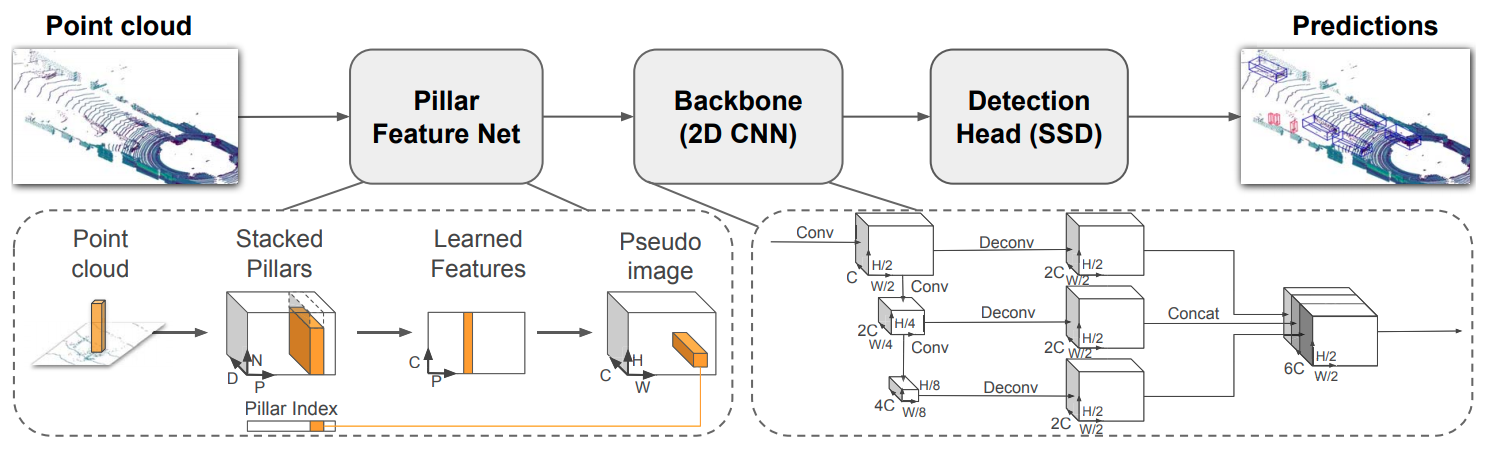
\includegraphics[width=1\textwidth]{figures/4_sistemas_de_percepcion_con_lidar_basados_en_deep_learning/pointpillars.png}
	\caption{Arquitectura propuesta del detector PointPillars.}
	\label{fig:Arquitectura_propuesta_del_detector_pointpillars}
\end{figure}

\newpage

\begin{enumerate}
\item Nube de puntos a pseudo im�genes\par
Se comienza voxelizando la nube de puntos formando diferentes pilares, esto quiere decir que cada v�xel tiene un tama�o $x$ e $y$ fijo pero en $z$ se tiene un tama�o infinito. Por cada punto en los v�xeles se les a�ade junto a las tres dimensiones con la informaci�n de posici�n: el grado de reflectividad, la distancia aritm�tica a la media de los puntos del v�xel en las tres dimensiones y el desplazamiento en $x$ e $y$ al centro del v�xel, por lo que se tiene un espacio de nueve dimensiones por pilar. Para limitar el c�mputo, se define un t�ma�o m�ximo por pilar de [9, n�mero de pilares no vac�os, n�mero de puntos por pilar], se esta manera se fija un m�ximo de n�meros de puntos por pilar y se aplica zero padding si el pilar se encuentra con muy poca informaci�n.\par
Tras esto se aplica una capa linear con batch normalization y una \acs{relu} seguido de una operaci�n de m�ximo por cada uno de los puntos del pilar para obtener un tensor de tama�o [X, n�mero de pilares no vac�os], lo cual es pasado a una pseudo imagen pasando el n�mero de pilares no vac�os a la altura y anchura de la imagen en funci�n de la posici�n de dichos pilares. Con lo que se consigue un estructura similar a la de una imagen \acs{bev}.
\item Backbone\par
Se utiliza un backbone similar al de VoxelNet \cite{voxelnet}, este backbone tiene dos subcapas, una que aumenta el n�mero de caracter�sticas a nivel espacial y otra que aumenta y relaciona las caracter�sticas de los pilares.
\item Cabeza detectora\par
En la salida se utiliza una \ac{ssd} para obtener las salidas de las detecciones 3D.
\end{enumerate}

Este enfoque de uso de \acs{cnn} sobre nubes de puntos de la misma manera que se analizar�a para im�genes, se ha visto en este paper, que es muy �til para acelerar la inferencia del modelo, adem�s que se consigue un muy buen rendimiento para tareas de detecci�n 3D y detecci�n \acs{bev} 2D.

\subsection{PointRCNN}
\label{sec:pointrcnn}

PointRCNN \cite{pointrcnn} propone un modelo basado en dos fases para la detecci�n de objetos 3D. Dichas fases consisten en una primera fase de generaci�n de las detecciones 3D y otra de refinamiento de las bounding boxes 3D.

\begin{figure}[H]
	\centering
	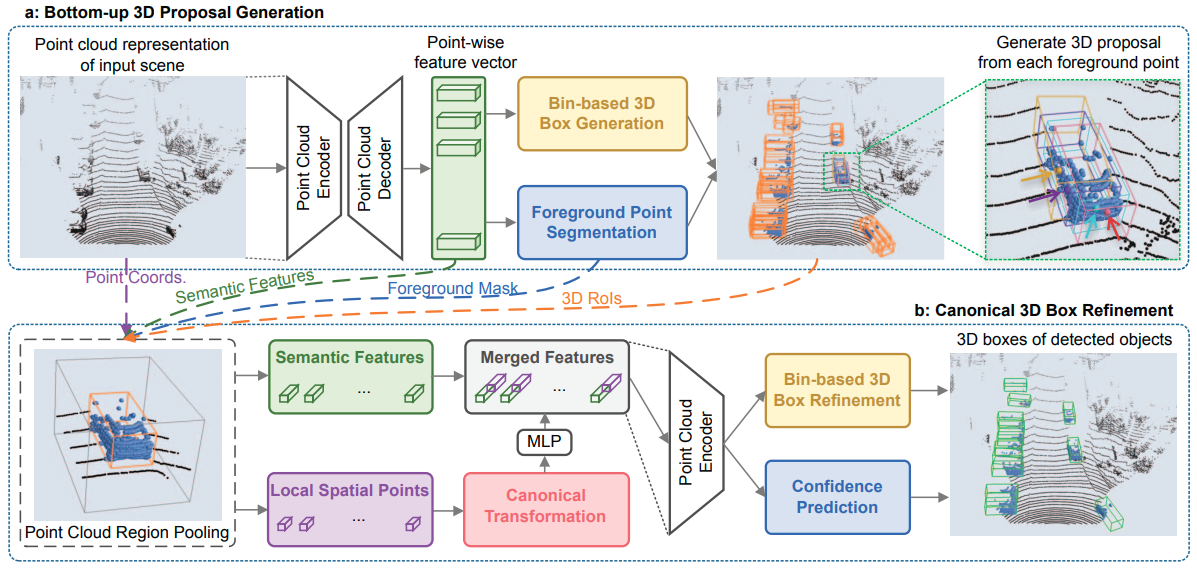
\includegraphics[width=0.8\textwidth]{figures/4_sistemas_de_percepcion_con_lidar_basados_en_deep_learning/pointrcnn.png}
	\caption{Arquitectura propuesta del detector PointRCNN.}
	\label{fig:Arquitectura_propuesta_del_detector_pointrcnn}
\end{figure}

El funcionamiento de las dos fases del modelo es el siguiente:

\begin{enumerate}
\item Generaci�n de propuestas de detecci�n 3D v�a segmentaci�n de la nube de puntos\par
La primera fase del modelo se basa en el backbone de PointNet++ \cite{pointnet++} para extraer las caracter�sticas a nivel de punto de la nube de puntos utilizando un agrupaci�n multiescala. Con dicho modelo junto con un m�todo propio basado en la discretizaci�n 2D en \acs{bev} (bin-based) se hayan las m�ltiples detecciones 3D, pero se reducen por cada objeto aplicando \ac{nms} basado en el \ac{iou} como \acs{bev} con un l�mite de 0,8 y solo las 100 mejores detecciones son mantenidas para la siguiente fase de ajuste de las detecciones 3D.
\item Refinamiento de las bounding boxes 3D\par
Tras la obtenci�n de las bounding boxes 3D, se trata de mejorar el centro y la orientaci�n de estas. Por cada una de dichas detecciones se aumenta su tama�o por un valor constante incluyendo adem�s una mascara que diferencia aquellos puntos de la detecci�n original al espacio aumentado. Cada una de dichas detecciones aumentadas pasan a utilizar el sistema de coordenadas propio de cada detecci�n.
\begin{figure}[H]
	\centering
	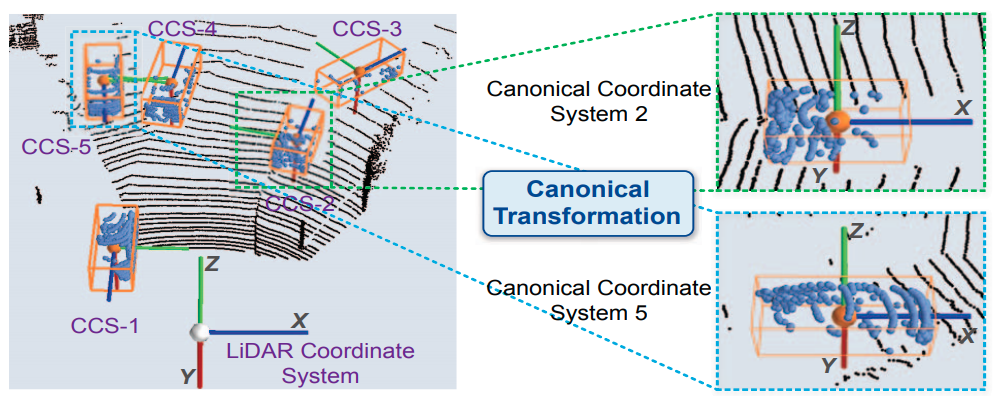
\includegraphics[width=0.6\textwidth]{figures/4_sistemas_de_percepcion_con_lidar_basados_en_deep_learning/region_pooling_pointrcnn.png}
	\caption{Agrupaci�n de regiones de la nube de puntos en el modelo PointRCNN.}
	\label{fig:Agrupacion_de_regiones_de_la_nube_de_puntos_en_el_modelo_pointrcnn}
\end{figure}
A partir de los puntos de cada agrupaci�n de las caracter�sticas extra�das de la primera fase y de un par�metro que agrega informaci�n de la distancia al sensor para aquellas agrupaciones con menos puntos calculado como $\sqrt{x�+y�+z�}$, se introducen en m�ltiples capas \acs{fc} para obtener las caracter�sticas locales. Tras esto se vuelve a utilizar el modelo bin-based utilizado en la primera fase con lo que se obtienen las bounding boxes 3D aplicando nuevamente \acs{nms} sobre un \acs{iou} en \acs{bev} con un l�mite de 0,01 para eliminar solapamientos.
\end{enumerate}

Al encontrarse basado este m�todo en dos subredes, sufre de un tiempo de computo mayor, lo que se traduce en una velocidad de 12 Hz \cite{rangercnn}, pero suficiente para aplicarse en tiempo real al obtener t�picamente las nubes de puntos a 10 Hz.

\subsection{PV-RCNN}
\label{sec:pv_rcnn}

PV-RCNN \cite{pv_rcnn} unifica los beneficios de las dos principales t�cnicas de detecci�n de objetos utilizando \acs{lidar}, como son: el uso de t�cnicas de voxelizaci�n junto con Sparse Convolutional Networks y el uso de backbones como el de PointNet \cite{pointnet} o m�todos similares. Para ello se construye un modelo basado en tres pasos:

\newpage

\begin{figure}[H]
	\centering
	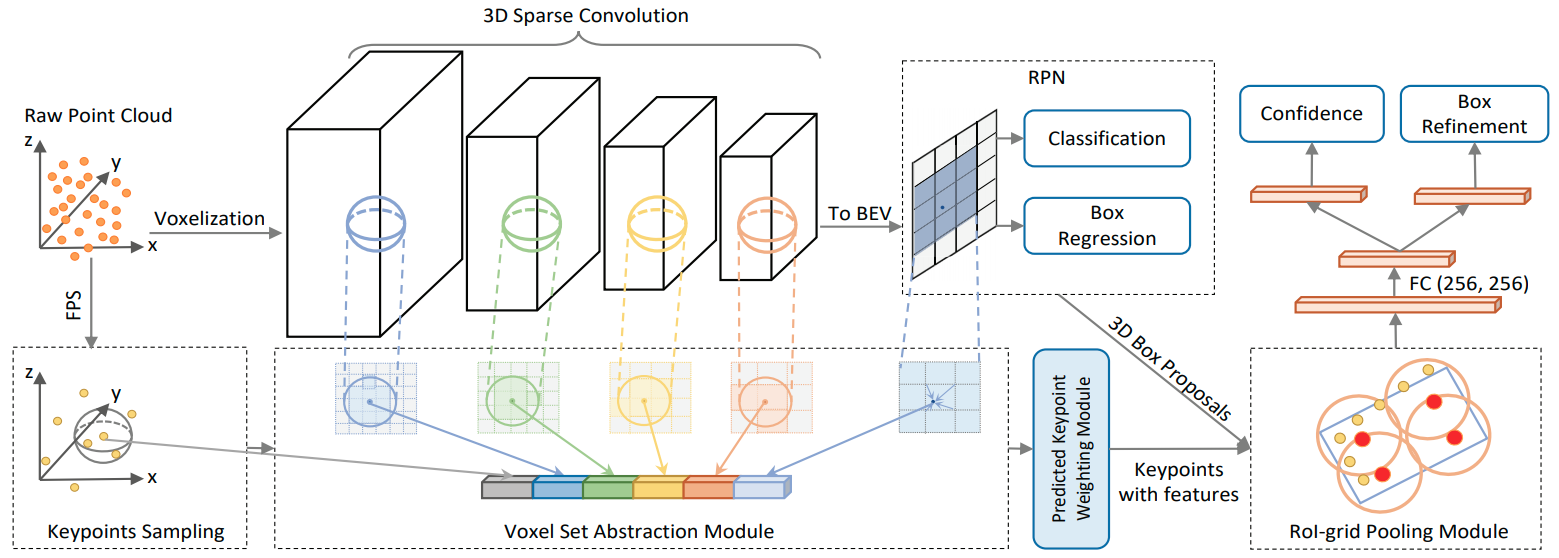
\includegraphics[width=0.8\textwidth]{figures/4_sistemas_de_percepcion_con_lidar_basados_en_deep_learning/pvrcnn.png}
	\caption{Arquitectura propuesta del detector PV-RCNN.}
	\label{fig:Arquitectura_propuesta_del_detector_pv_rcnn}
\end{figure}

\begin{enumerate}
\item 3D Voxel \acs{cnn} para la extracci�n de caracter�sticas y generaci�n de detecciones\par
Se utiliza una Voxel \acs{cnn} con 3D sparse convolution junto con una \acs{rpn}, la cual es una elecci�n popular en el \acs{sota} gracias a su eficiencia, por lo que es el backbone utilizado utilizado en este modelo. Este m�todo obtiene de forma interna caracter�sticas sem�nticas de los v�xeles adem�s de conseguir las detecciones de los objetos a partir de los tama�os prefijados o anchors.
\item Codificaci�n de escenas de v�xel a puntos clave\par
Primero se agregan las caracter�sticas de los v�xeles en un conjunto de puntos clave que sirven de conexi�n entre la fase anterior y el refinamiento de las detecciones. Para la obtenci�n de los puntos clave se adopta el algoritmo Furthest Point Sampling y se aplica sobre la nube de puntos, lo cual elige puntos de forma uniformemente distribuida sobre los v�xeles no vac�os. Tras esto se propone el m�dulo Voxel Set Abstraction para codificar caracter�sticas sem�nticas de la primera fase en los puntos clave. Bas�ndose en la premisa de que los puntos m�s cercanos tiene que contribuir m�s a la propuesta de detecci�n se propone el m�dulo Predicted Keypoint Weighting.
\begin{figure}[H]
	\centering
	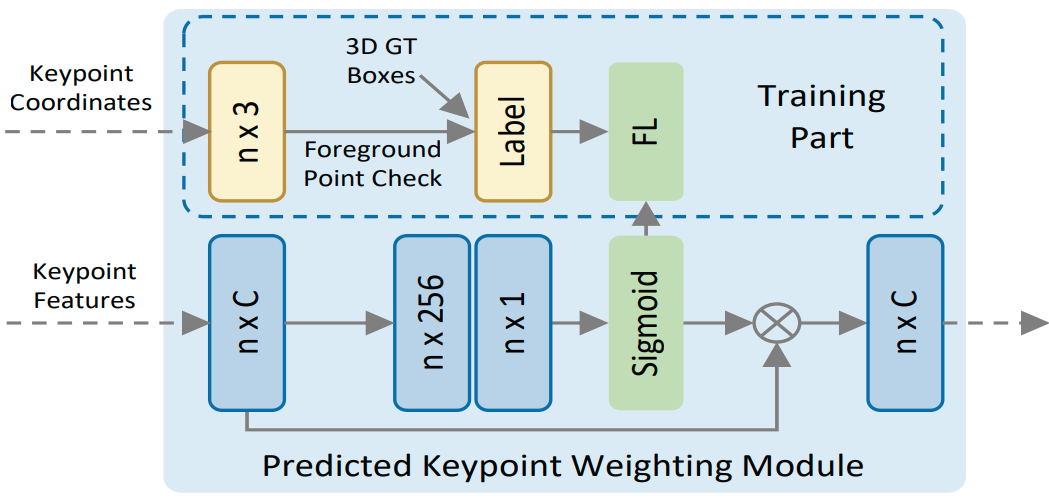
\includegraphics[width=0.5\textwidth]{figures/4_sistemas_de_percepcion_con_lidar_basados_en_deep_learning/pkw_pvrcnn.png}
	\caption{M�dulo Predicted Keypoint Weighting del modelo PV-RCNN.}
	\label{fig:Agrupacion_de_regiones_de_la_nube_de_puntos_en_el_modelo_pc_rcnn}
\end{figure}
En dicho m�dulo se introducen los puntos clave codificados previamente para dar un peso a cada uno en funci�n de su importancia para las detecciones.
\item Abstracci�n de caracter�sticas de \acs{roi} de puntos clave a cuadr�cula para el refinamiento de la detecci�n\par
Para el refinamiento de las detecciones se utiliza un m�todo de abstracci�n de caracter�sticas \acs{roi} de puntos clave a rejilla. Dadas las detecciones junto con los puntos codificados y sus pesos, se agregan entorno a diferentes puntos de rejilla con un radio determinado. Tras esto se obtienen las caracter�sticas de las rejillas y a partir de estas, con una peque�a red de dos capas se ajusta la detecci�n.
\end{enumerate}

De la misma manera que ocurr�a en PointRCNN, PV-RCNN tiene una velocidad de inferencia baja de 10 Hz \cite{rangercnn} debido a la fase de refinamiento y el procesamiento adicional de las caracter�sticas del backbone.

\subsection{CBGS}
\label{sec:cbgs}

Class-balanced Grouping and Sampling (CBGS) \cite{cbgs} propone un modelo compuesto principalmente de 4 partes: m�dulo de entrada, extractor de caracter�sticas 3D, \acs{rpn} y una red con m�ltiples cabeceras en funci�n del grupo. Con esto se consigue un funcionamiento en detecci�n 3D, predicci�n de la velocidad y de la clase, todo ello sobre las 10 clases diferentes que utiliza nuScenes.

\begin{figure}[H]
	\centering
	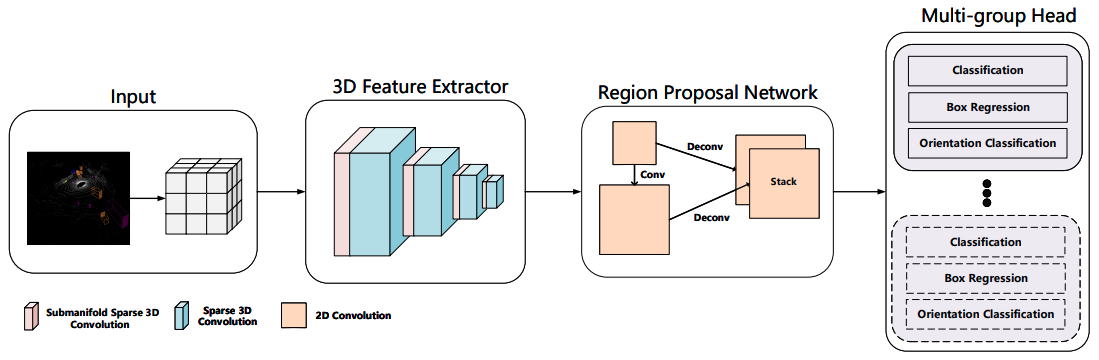
\includegraphics[width=0.8\textwidth]{figures/4_sistemas_de_percepcion_con_lidar_basados_en_deep_learning/cbgs.png}
	\caption{Arquitectura propuesta del detector CBGS.}
	\label{fig:Arquitectura_propuesta_del_detector_pv_rcnn}
\end{figure}

Parte del funcionamiento del modelo proviene de la fase de entrenamiento, en la que se aplica una t�cnica de muestreo que trata de mejorar la media de uso de las diferentes clases para reducir la irregularidad del dataset de nuScenes, lo que aumenta el conjunto de entrenamiento de 28.130 a 128.100 muestras.\par
Para realizar la inferencia en el modelo se siguen los siguientes pasos:

\begin{enumerate}
\item Entrada de la red\par
Debido al m�todo de validaci�n de las detecciones en nuScenes es necesaria la inferencia de la velocidad por lo que siguiendo el m�todo oficial del dataset, se utilizan diez barridos de \acs{lidar} para la obtenci�n del dato de la velocidad. En la entrada del modelo es necesario entonces alguna medida de tiempo, por lo que cada punto se encuentra codificado como [$x$, $y$, $z$, $intensity$, $\Delta t$], siendo $\Delta t$ la diferencia de tiempo entre el barrido inicial y el barrido del que proviene el punto. Tras esto se voxeliza la nube de puntos con un tama�o de v�xel de [0.1, 0.1, 0.2] m para la reducci�n del tiempo de computo. Dentro de cada v�xel se mantiene unicamente la media de todos puntos de dicho v�xel.
\item Backbone utilizado\par
En la red principal es utilizado un modelo basado en sparse 3D convolution y un extractor de caracter�sticas. Tras esto se aplica un \acs{rpn}, lo que termina en una red similar a la de VoxelNet \cite{voxelnet} para extraer m�s caracter�sticas pero con capas convolucionales 2D.
\item Class-balance Grouping\par
Al tener una aparici�n de las diferentes clases muy irregular, con casi un 45\% de los objetos siendo coches, es muy dif�cil para objetos con formas diferentes extraer las diferencias entre ellos. Por ejemplo una bicicleta y una motocicleta tienen una forma muy similar en lo que respecta a la nube de puntos, al igual que ocurren con un cami�n y un cami�n de construcci�n. Para solucionar este problema se propone la agrupaci�n de clases en funci�n de su similitud, teniendo en cuenta el tama�o de los objetos y un balanceo del tama�o de los grupos en funci�n del n�mero de clases. Lo cual acaba generando 6 grupos diferentes: (Coche), (Cami�n, Cami�n de construcci�n), (Bus, Tr�iler), (Barrera), (Motocicleta, Bicicleta), (Peat�n, Cono de tr�fico). Por lo que tras la elecci�n del grupo, se obtiene su cabecera y se hayan la posici�n, tama�o, rotaci�n y velocidad.
\end{enumerate}

Este m�todo consigue por tanto una detecci�n de objetos 3D adem�s de un pseudo tracking para inferir la velocidad de los objetos, todo ello trabajando con 10 clases diferentes y obteniendo una velocidad de 9 Hz.

\section{OpenPCDet}
\label{sec:openpcdet}

OpenPCDet \cite{openpcdet} es un proyecto Open-Source para realizar detecciones de objetos 3D utilizando \acs{lidar}. Esta herramienta ha sido utilizada para la evaluaci�n, entrenamiento e implementaci�n de diversos modelos debido a la diversidad de modelos y de datasets que son soportados.\par
OpenPCDet es un repositorio en Pytorch \cite{pytorch} que soporta m�ltiples modelos \acs{sota} en detecci�n de objetos 3D, con un c�digo altamente refactorizado para las arquitecturas basadas en una o dos etapas. Este repositorio de c�digo abierto es activamente actualizado con nuevos datasets soportados y modelos. Basado en OpenPCDet se ha conseguido ganar el Waymo Open Dataset en detecci�n 3D, seguimiento 3D y adaptaci�n del entorno utilizando unicamente las nubes de puntos del \acs{lidar}.

\begin{figure}[H]
	\centering
	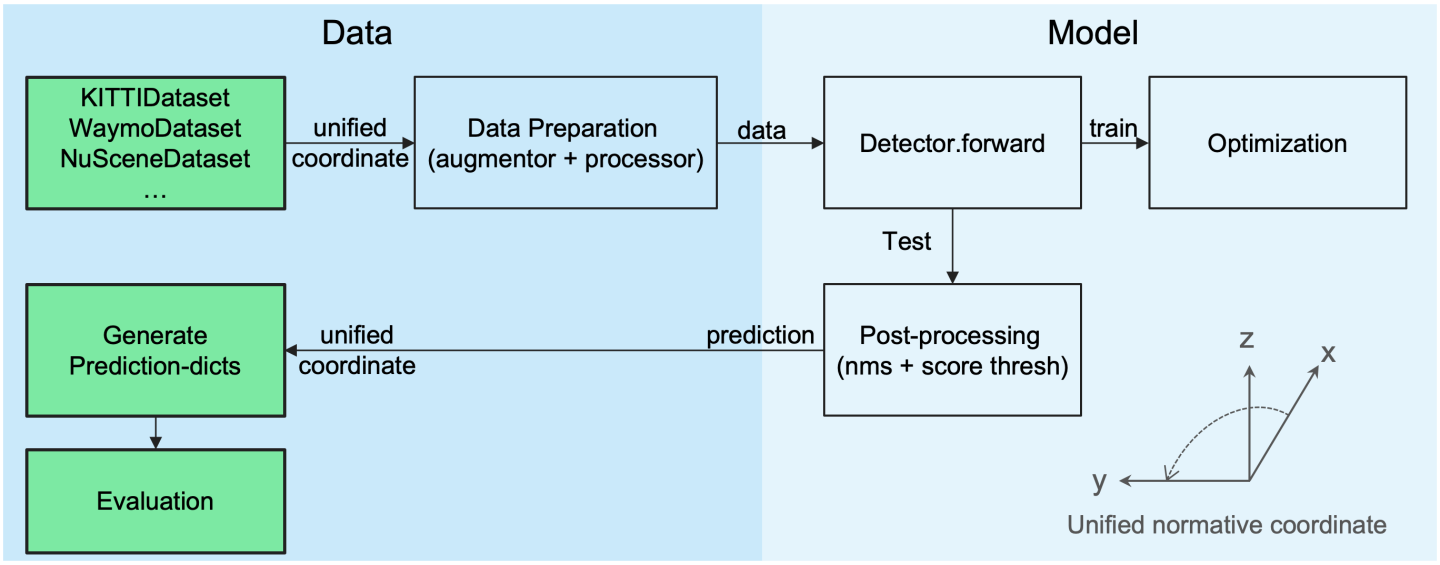
\includegraphics[width=0.7\textwidth]{figures/4_sistemas_de_percepcion_con_lidar_basados_en_deep_learning/openpcdet.png}
	\caption{Dise�o de OpenPCDet.}
	\label{fig:Dise�o_de_openpcdet}
\end{figure}

El patr�n de dise�o de OpenPCDet se encuentra basado en: la separaci�n de datos a modelo unificando el sistema de coordenadas, definici�n �nica de las bounding boxes 3D [$x$, $y$, $z$, $dx$, $dy$, $dz$, $heading$], definici�n de la estructura de los modelos clara y flexible permitiendo f�cilmente el soporte de m�ltiples modelos. Esta herramienta incluye diversos modelos en diferentes datasets, estos son:

\begin{itemize}
\item KITTI \cite{kitti_dataset}
	\begin{itemize}
	\item PointPillars \cite{pointpillars}
	\item SECOND \cite{second}
	\item PointRCNN \cite{pointrcnn}
	\item Part-A$�$ \cite{part-a2}
	\item PV-RCNN \cite{pv_rcnn}
	\item Voxel R-CNN \cite{voxel_rcnn}
	\item CaDDN \cite{caddn}
	\end{itemize}
\item nuScenes \cite{nuscenes_dataset}
	\begin{itemize}
	\item CBGS \cite{cbgs}
	\end{itemize}
\item Waymo \cite{waymo_dataset}
	\begin{itemize}
	\item SECOND \cite{second}
	\item Part-A$�$ \cite{part-a2}
	\item PV-RCNN \cite{pv_rcnn}
	\end{itemize}
\end{itemize}

Para el uso principal de la herramienta se utilizan los ficheros \textit{train.py} y \textit{test.py}, con estos a partir de diferentes flags es posible entrenar y evaluar los diferentes modelos que se deseen, sin necesidad de limitarse a los modelos que se tienen implementados, sino que dentro de \textit{OpenPCDet/tools/cfgs} es posible modificar los ya existentes o tambi�n es posible crear nuevos modelos a partir de objetos en Python que utilicen toda la flexibilidad que OpenPCDet ofrece para reutilizar m�dulos de otros modelos.\par
Todo esto convierte a OpenPCDet en una gran herramienta para el desarrollo de modelos que sean basados en el \acs{sota}, como herramienta de evaluaci�n o para la implementaci�n de modelos ya creados.


\chapter{Desarrollo realizado}
\label{cha:desarrollo_realizado}

\begin{FraseCelebre}
  \begin{Frase}
    La persistencia es muy importante. No debes renunciar al menos que te veas obligado a renunciar.
  \end{Frase}
  \begin{Fuente}
    Elon Musk
  \end{Fuente}
\end{FraseCelebre}

\noindent
Tras el estudio te�rico de los m�todos cl�sicos y basados en Deep Learning se procede a explicar el desarrollo realizado en el contexto del proyecto Techs4AgeCar dentro del grupo Robesafe para la mejora del sistema de percepci�n, tanto utilizando unicamente el \acs{lidar} como en base a una fusi�n sensorial entre c�mara y \acs{lidar}.

\section{Estado del proyecto Techs4AgeCar}
\label{sec:estado_del_proyecto_t4ac}

El proyecto Techs4AgeCar trata de construir un sistema de conducci�n aut�noma, con una arquitectura basada en m�ltiples capas como son: localizaci�n, planificaci�n, control, mapeado, decisi�n y percepci�n. Para el desarrollo del software del veh�culo se trabaja con \acs{ros} para comunicaci�n con los sensores y entre capas, Docker para tener un entorno cerrado con todas las dependencias y software necesario para correr el proyecto y CARLA como entorno de simulaci�n para las pruebas de los m�ltiples sistemas del veh�culo.

\subsection{Robot Operating System}
\label{sec:ros}

\ac{ros} \cite{ros} es un conjunto de librer�as software y herramientas Open-Source que ayudan con la construcci�n de aplicaciones en robots. Aunque el nombre indicar�a que este es un sistema operativo, no lo es, sino que es un software middleware que provee de abstracci�n del hardware, control de dispositivos a bajo nivel, implementaci�n de funcionalidades com�nmente utilizadas, paso de mensajes entre procesos y gesti�n de paquetes. Adem�s de esto esto se proveen de herramientas y librer�as para obtener, construir, escribir y correr c�digo en diferentes ordenadores.\par
La meta principal de \acs{ros} es la reutilizaci�n de c�digo en rob�tica de investigaci�n y desarrollo. \acs{ros} utiliza un marco distribuido de procesos que permite la ejecuci�n de cada uno de forma individual

\begin{figure}[H]
	\begin{minipage}{0.48\textwidth}
		\centering
		
\includegraphics[width=0.7\linewidth]{figures/5_desarrollo_realizado/ros_logo.png}
		\caption{Logo de ROS.}
		\label{fig:Logo_de_ros}
	\end{minipage}\hfill
	\begin{minipage}{0.48\textwidth}
		\centering
		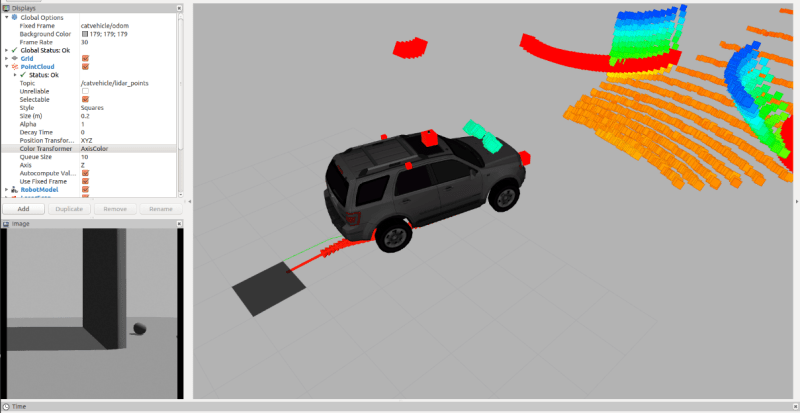
\includegraphics[width=1\linewidth]{figures/5_desarrollo_realizado/ros_example.png}
		\caption{Ejemplo de uso de ROS}
		\label{fig:Ejemplo_de_uso_de_ros}
	\end{minipage}
\end{figure}

La forma de comunicaci�n de \acs{ros} es mediante un modelo peer-to-peer de procesos que se encuentran d�bilmente acoplados. Los principales conceptos del grafo de computo de \acs{ros} son los siguientes:

\begin{itemize}
\item Nodos\par
Los nodos suelen ser lo t�picos procesos que realizan el computo. Dichos nodos son escritos mediante la librer�a del cliente de \acs{ros} utilizando roscpp para C++ o rospy para Python.
\item Maestro\par
El maestro permite que los nodos se pueden encontrar, intercambiar mensajes y permite invocar los servicios.
\item Servidor de par�metros\par
El servidor de par�metros permite almacenar los datos por clave, encontr�ndose este dentro del maestro.
\item Mensajes\par
Los mensajes son estructuras de datos con ciertos atributos, dichas estructuras son  utilizadas para la comunicaci�n entre nodos, y a�n teniendo mensajes est�ndares es posible crear nuevos que se adapten a las necesidades de cada problema.
\item Topics\par
Mientras que un mensaje es unicamente la estructura de datos, los topics identifican los mensajes en funci�n de un nombre. Estos topics son accedidos mediante suscripciones para la lectura de mensajes  y publicaciones para la escritura de mensajes, todo ello a trav�s de topics. Por lo que son utilizados por los nodos para trabajar con los mensajes.
\item Servicios\par
El modelo de publicaci�n y suscripci�n es utilizado para la comunicaci�n bajo un modelo many-to-many, para utilizar un modelo en una direcci�n no es recomendable, por ello en ese caso se utilizan servicios. Los servicios se basan en cambio en un modelo de solicitud y respuesta, por lo que mientras un nodo ofrece un servicio bajo un nombre, otro nodo puede acceder a dicho servicio.
\item Bags\par
Los bags son el formato utilizado por \acs{ros} para guardar y recrear de nuevo los mensajes grabados. Estos son utilizados para la recreaci�n, comparativa o evaluaci�n a partir de los datos grabados.
\end{itemize}

\begin{figure}[H]
	\centering
	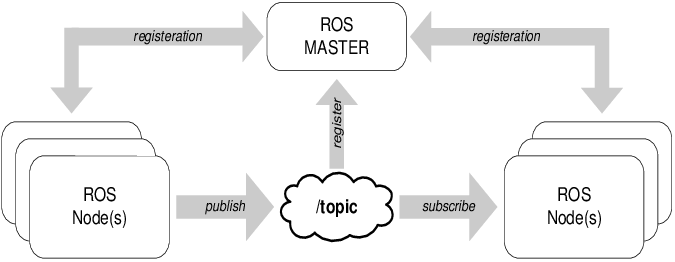
\includegraphics[width=0.6\textwidth]{figures/5_desarrollo_realizado/graph_ros.png}
	\caption{Funcionamiento principal de ROS.}
	\label{fig:Funcionamiento_principal_de_ros}
\end{figure}

De esta manera \acs{ros} consigue ser un sistema distribuido con m�ltiples aplicaciones. Solo es necesario tener en cuenta que se encuentra disponible en sistemas basados en Unix como Ubuntu y MacOS, aunque es sencillo encontrar soporte para otras distribuciones basadas en Linux \cite{ros_wiki}.

\subsection{Docker}
\label{sec:docker}

Docker \cite{docker} es un proyecto Open-Source que automatiza el despliegue de aplicaciones dentro de contenedores de software, proporcionando una capa de abstracci�n y automatizaci�n de la virtualizaci�n de aplicaciones en m�ltiples sistemas operativos \cite{docker_wikipedia}.\par
El aislamiento y la seguridad son elementos principales de la herramienta, la cual permite la ejecuci�n de m�ltiples contenedores en un �nico host. Dichos contenedores son ligeros y contienen todo lo necesario para la ejecuci�n de las aplicaciones, por lo que no hay ninguna dependencia del host en el que se est� ejecutando. Adem�s se pueden compartir los contenedores de forma muy sencilla haciendo uso de Docker Hub con un funcionamiento basado en push/pull.\par
Docker es utilizado para agilizar el ciclo de desarrollo de software, permitiendo trabajar en entornos estandarizados utilizando contenedores locales que proporcionan las aplicaciones y servicios. Por lo tanto los contenedores de Docker son una gran herramienta para los flujos de trabajo de integraci�n y entrega continua.

\begin{figure}[H]
	\centering
	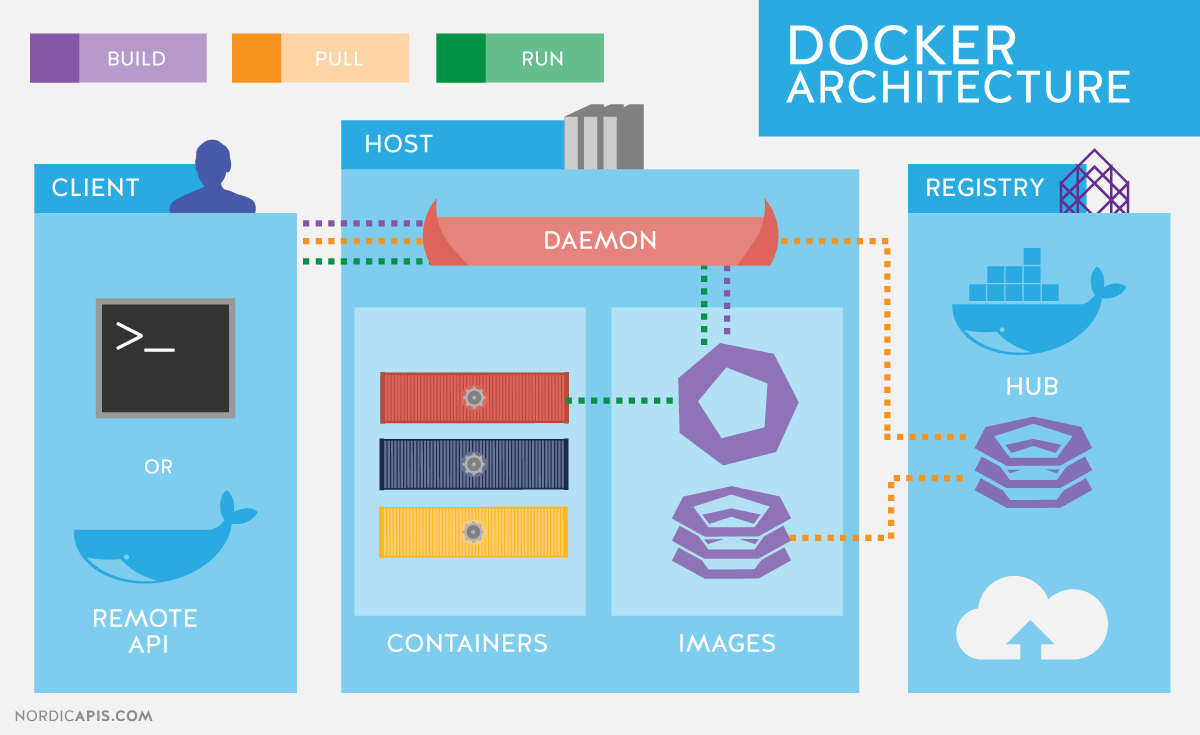
\includegraphics[width=0.6\textwidth]{figures/5_desarrollo_realizado/docker_architecture.png}
	\caption{Arquitectura de Docker.}
	\label{fig:Arquitectura_de_docker}
\end{figure}

Docker utiliza una arquitectura cliente-servidor. El cliente habla con el daemon, el cual hace el trabajo de construir ejecutar y distribuir los contenedores. Tanto el cliente como el daemon suelen encontrarse en el mismo sistema, pero tambi�n se puede trabajar con un daemon de forma remota, para ello se utiliza una comunicaci�n basada en una REST API sobre sockets UNIX u otra interfaz de red.\par
Los principales componentes de la arquitectura de Docker son los siguientes:

\begin{itemize}
\item Daemon\par
El daemon escucha a las peticiones de la \acs{api} de Docker y gestiona los objetos de Docker como im�genes, contenedores, redes y vol�menes. Adem�s los daemons pueden comunicarse a otros daemons para controlar servicios.
\item Cliente\par
El cliente es el principal m�todo de uso de Docker por muchos usuarios para trabajar con im�genes o contenedores. El cliente se conecta a un daemon pero tambi�n es posible su conexi�n a m�ltiples daemon diferentes.
\item Registros\par
Los registros son utilizados para guardar las im�genes de Docker. Un caso de registro p�blico ser�a Docker Hub donde se pueden guardar y descargar las im�genes creadas.
\item Im�genes\par
Una imagen es una plantilla de solo lectura que se utiliza para crear un contenedor. A partir de una imagen se descarga e instala todo el software necesario para que el contenedor funcione correctamente, y en el caso de tener que crear una imagen propia se utilizan \textit{Dockerfiles}, que son archivos con una sintaxis sencilla que definen los pasos necesarios para crear la imagen y correrla.
\item Contenedores\par
Un contenedor es una instancia ejecutable de una imagen. Sobre un contenedor se pueden aplicar las opciones de crear, ejecutar, pausa, mover y borrar utilizando la \acs{api} de Docker o \acs{cli}. Es posible la conexi�n a un contenedor en otra red o incluso crear im�genes de forma autom�tica a partir del estado de un contenedor.
\end{itemize}

Docker se encuentra escrito en lenguaje Go y utiliza m�ltiples caracter�sticas del kernel de Linux para ofrecer sus funcionalidades. Docker utiliza un sistema de \textit{namespaces} que proveen de una capa de aislamiento al contenedor respecto del host, por lo que los contenedores corren de forma separada a fuera de ese \textit{namespace} y su acceso se encuentra limitado al interior de este \cite{docker_docs}.

\subsection{CARLA}
\label{sec:CARLA}

CARLA \cite{carla} es un simulador de conducci�n aut�noma Open-Source. Este simulador sirve como un entorno en el que probar diversas t�cnicas necesarias para la conducci�n aut�noma mediante el uso de la \acs{api} que se ofrece en Python y C++. CARLA se encuentra basado en el motor de videojuegos Unreal Engine \cite{unrealengine} para correr el mundo y utiliza el est�ndar OpenDRIVE \cite{opendrive} para la definici�n de carreteras y el entorno.\par
Unreal Engine 4 es la versi�n utilizada por CARLA, este motor de videojuegos es desarrollado por Epic Games. Inicialmente para videojuegos, Unreal Engine se ha extendido en otras industrias como la televisi�n y el mercado cinematogr�fico. Escrito en C++, Unreal Engine ofrece gran portabilidad en una gran cantidad de dispositivos, con un modelo Open-Source pero con royalties en el uso comercial. Con el �xito de Fornite, muchos juegos est�n utilizando este motor gr�fico lo que ha aumentado el desarrollo de la siguiente versi�n de Unreal Engine, la cual se espera en 2022 con una gran mejora gr�fica.

\begin{figure}[H]
	\centering
	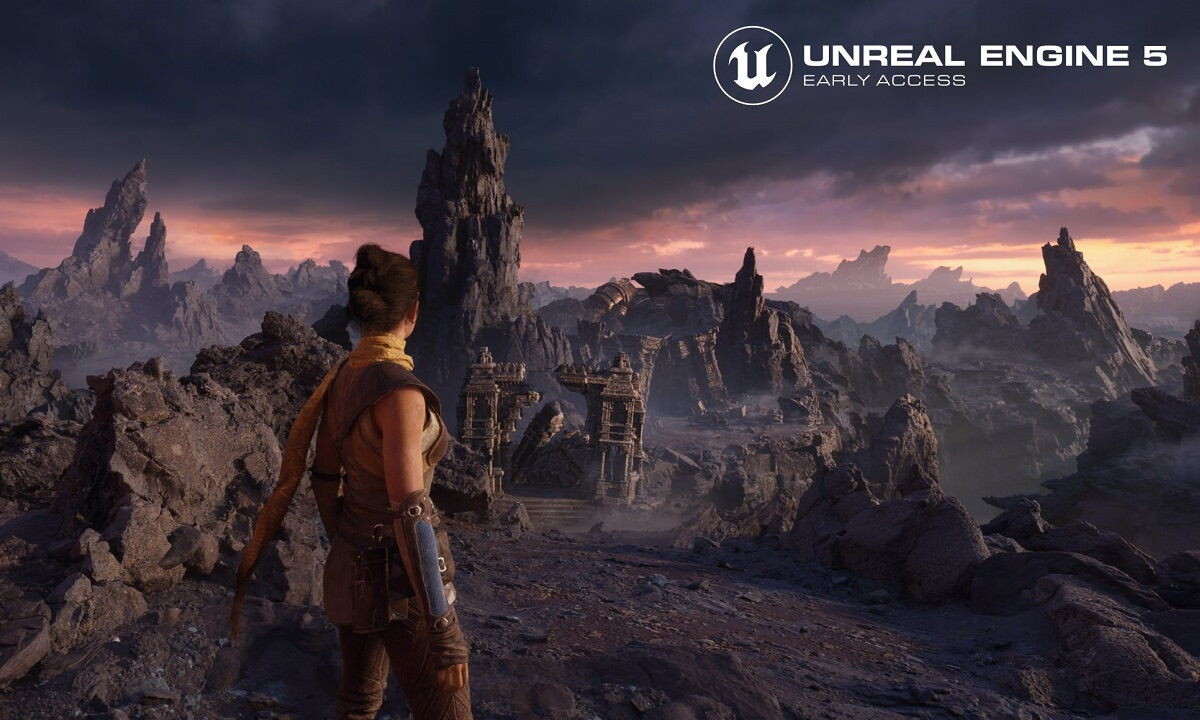
\includegraphics[width=0.55\textwidth]{figures/5_desarrollo_realizado/unreal_engine_5.jpeg}
	\caption{Unreal Engine 5.}
	\label{fig:Unreal_engine_5}
\end{figure}

OpenDRIVE es un formato abierto para la creaci�n de redes de carreteras que trata de convertirse en el est�ndar la creaci�n de mapas y sistemas de carreteras para facilitar el uso de diferentes mapas y simuladores. Los mapas creados con OpenDRIVE utilizan la extensi�n \textit{.xodr} y dichos archivos utilizan un formato similar al \acs{xml} para su uso simplificado con herramientas ya creadas.\par
Para la aceleraci�n del proceso de desarrollo, entrenamiento y validaci�n de los \acs{ads}, CARLA ha creado un ecosistema de proyectos a partir del simulador en conjunto con la comunidad que utiliza CARLA.\par
CARLA utiliza un modelo cliente-servidor como arquitectura. El servidor es responsable de toda la simulaci�n: renderizaci�n de los sensores, c�lculo de las f�sicas, actualizaci�n del mundo, etc. Con todos estos c�lculos es recomendado el uso de una \acs{gpu}, sobre todo si se utilizan t�cnicas basadas en Deep Learning. Por otra parte, el cliente es aquel que controla la l�gica de los actores en la escena y cambia las opciones del mundo, de esta manera se pueden tener m�ltiples clientes trabajando al mismo tiempo. La comunicaci�n al servidor se realiza mediante la \acs{api} que provee CARLA, pero tambi�n es posible utilizar el CARLA-ROS bridge para utilizar los topics de \acs{ros} para la comunicaci�n \cite{carla_intro}.

\begin{figure}[H]
	\centering
	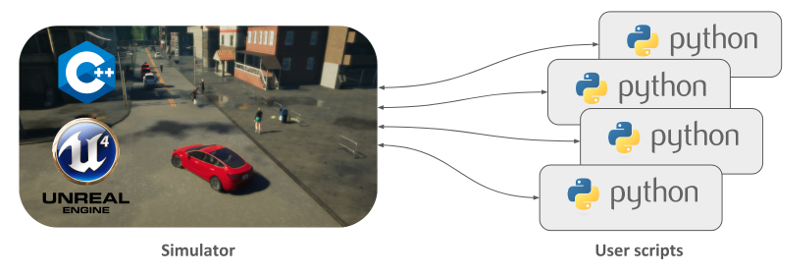
\includegraphics[width=0.8\textwidth]{figures/5_desarrollo_realizado/carla_modules.png}
	\caption{Modo de uso principal de CARLA.}
	\label{fig:Modo_de_uso_principal_de_carla}
\end{figure}

CARLA ofrece una comunicaci�n entre este y ROS, dicho m�dulo que permite esto es el CARLA-ROS bridge. El funcionamiento de este se basa en el paso de la informaci�n que ser�a accesible a partir de la \acs{api} de CARLA mediante mensajes publicados en diversos topics en ROS. Dicho CARLA-ROS bridge funciona en ambas versiones de \acs{ros} y publica de forma continua:
\begin{itemize}
\item Informaci�n de diversos sensores del coche controlado como son: c�mara (profundidad, segmentaci�n a nivel de p�xel y RGB), \acs{lidar}, \acs{radar}, \acs{gnss} e \acs{imu}
\item Informaci�n de los objetos del entorno como: estado de los sem�foros, indicadores de colisi�n, invasi�n de carril, etc.
\item Control del veh�culo aut�nomo como: direcci�n, aceleraci�n y freno
\item Control de los ajustes generales del simulador
\end{itemize}

CARLA ofrece por tanto un simulador Open-Source, con una gran comunidad de desarrolladores aportando al desarrollo de este, por lo que es una herramienta perfecta para la evaluaci�n de los sistemas de conducci�n aut�noma a desarrollar.

\subsection{Desarrollo en el proyecto Techs4AgeCar}
\label{sec:Desarrollo_en_el_proyecto_t4ac}

El proyecto Techs4AgeCar trata de construir un veh�culo aut�nomo que consiga una mejora para la seguridad de los conductores. A�n teniendo un gran desarrollo en la parte hardware del proyecto para la construcci�n del veh�culo, el desarrollo de este TFG es software, por lo que se explica el uso de las diferentes herramientas utilizadas para el trabajo con un entorno estandarizado para todos los compa�eros, y como se ha trabajado en el desarrollo de las diversas t�cnicas implementadas.

\begin{figure}[H]
	\begin{forest}
	for tree={
    	font=\ttfamily,
        grow'=0,
        child anchor=west,
        parent anchor=south,
        anchor=west,
        calign=first,
        inner xsep=7pt,
        edge path={
        	\noexpand\path [draw, \forestoption{edge}]
          	(!u.south west) +(7.5pt,0) |- (.child anchor) pic {folder} \forestoption{edge label};
        },
        % style for your file node 
        file/.style={edge path={\noexpand\path [draw, \forestoption{edge}]
          	(!u.south west) +(7.5pt,0) |- (.child anchor) \forestoption{edge label};},
        	inner xsep=2pt,font=\small\ttfamily
                     },
        before typesetting nodes={
        	if n=1
            {insert before={[,phantom]}}
            {}
        },
        fit=band,
        before computing xy={l=15pt},
	}  
    [/home/robesafe
      [carla
      ]
      [libraries
      ]
      [models
      ]
      [shared\_home
      ]
      [t4ac\_ws
      	[build
      	]
      	[devel
      	]
      	[src
      	  [t4ac\_architecture
      	  	[t4ac\_config\_layer
      	  	]
      	  	[t4ac\_control\_layer
      	  	]
      	  	[t4ac\_decision\_making\_layer
      	  	]
      	  	[t4ac\_localization\_layer
      	  	]
      	  	[t4ac\_mapping\_layer
      	  	]
      	  	[t4ac\_perception\_layer
      	  	]
      	  	[t4ac\_planning\_layer
      	  	]
    	  ]
    	  [t4ac\_carla\_simulator
    	  	[ad\_devkit
    	  	]
    	  	[t4ac\_carla\_ros\_bridge
    	  	]
    	  	[t4ac\_carla\_scenario\_runner
    	  	]
    	  ]
		]
	  ]
    ]
	\end{forest}
\caption{Estructura principal del proyecto Techs4AgeCar en Docker.}
\label{for:Estructura_principal_del_proyecto_t4ac_en_docker}
\end{figure}

Para uso de un entorno estandarizado para todos los usuario se utiliza un contenedor Docker alojado en Docker Hub, que contiene todas las dependencias necesarias para correr el proyecto o sus componentes individuales. La �nica herramienta utilizada en el proyecto que se debe de encontrar fuera del contenedor es el simulador CARLA, que es necesario descargarlo fuera de este.\par
La figura \ref{for:Estructura_principal_del_proyecto_t4ac_en_docker} muestra de manera simplificada la estructura del docker del proyecto. En dicho contenedor se tiene instalado de base Ubuntu 18.04 LTS para trabajar sobre este sistema operativo. La estructura del contenedor consta del simulador CARLA, las librer�as o repositorios necesarios, los modelos de las redes neuronales utilizadas y la estructura principal de los diferentes m�dulos del proyectos. Por una parte se encuentra la carpeta \textit{t4ac\_architecture}, la cual contiene los repositorios de las diferentes capas del veh�culo junto con los ajustes de configuraci�n de todas estas. En la carpeta \textit{t4ac\_carla\_simulator} se encuentran los ajustes de carla, el Carla-ROS bridge ajustado al proyecto y un proyecto basado en CARLA llamado ad\_devkit para evaluaci�n de arquitecturas de conducci�n aut�noma del que se hablar� m�s en el cap�tulo \ref{cha:ad_devkit}.\par
Las diferentes capas del proyecto contenidas en \textit{t4ac\_architecture} son construidas como repositorios Git alojados en GitHub y en un servidor propio del grupo RobeSafe. Cada uno de estos repositorios se encuentran divididos en diferentes repositorios, por ejemplo en la capa de control se dividen seg�n el uso de t�cnicas cl�sica o basadas en Deep Learning, o en la capa de percepci�n se divide seg�n el uso de t�cnicas de detecci�n o seguimiento y en funci�n de los diferentes sensores.

\begin{figure}[H]
	\centering
	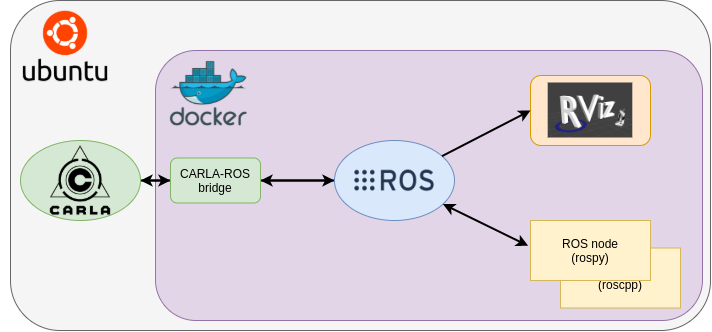
\includegraphics[width=0.9\textwidth]{figures/5_desarrollo_realizado/funcionamiento_proyecto.png}
	\caption{Modo de uso en el proyecto Techs4AgeCar.}
	\label{fig:Modo_de_uso_en_el_proyecto_t4ac}
\end{figure}

Los repositorios de las diferentes capas se encuentran planteados como nodos de \acs{ros} para trabajar con el simulador CARLA se pueda controlar el veh�culo, de esta manera como con el veh�culo del grupo RobeSafe se obtiene la informaci�n de los sensores a partir de ROS, solo es necesario un cambio en el topic para que funcione de simulaci�n al veh�culo real. En la figura \ref{fig:Modo_de_uso_en_el_proyecto_t4ac} se puede ver el principal modo de uso del proyecto donde CARLA se corre en el host y el resto del proyecto se lanza en el contenedor Docker. Dentro del contenedor se pasa la informaci�n de CARLA a ROS, dicha informaci�n es visualizada con rviz y los nodos de las diferentes capas en Python o C++ son corridos trabajando con el modelo publisher/subscriber de ROS.

\subsection{Arquitectura del proyecto Techs4AgeCar}
\label{sec:Arquitectura_del_proyecto_t4ac}

El grupo RobeSafe comienza a trabajar en la construcci�n de un veh�culo aut�nomo en 2016 con el proyecto SmartElderlyCar con finalizaci�n en 2018, tras este se continua con el proyecto Techs4AgeCar con una duraci�n del 2019 a 2021, y que pretende mejorar las t�cnicas de conducci�n aut�noma que se consiguieron con el proyecto anterior.\par
La lineas de investigaci�n del grupo son por tanto: \acl{adas}, comprensi�n de la escena, comprensi�n del comportamiento del conductor, desarrollo de t�cnicas de percepci�n, localizaci�n, navegaci�n y mapeado.

\begin{figure}[H]
	\centering
	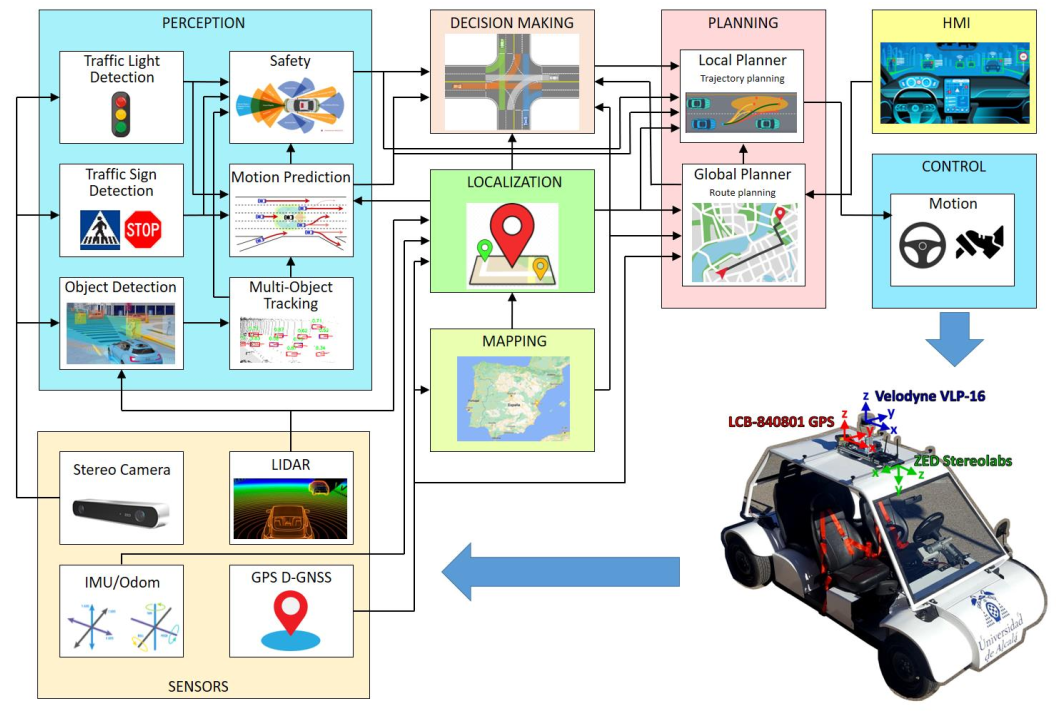
\includegraphics[width=0.7\textwidth]{figures/5_desarrollo_realizado/arquitectura_t4ac.png}
	\caption{Arquitectura T4AC.}
	\label{fig:Arquitectura T4AC}
\end{figure}

La arquitectura definida en el proyecto consta de diferentes capas en la que cada una realiza una funci�n diferente para el funcionamiento aut�nomo del veh�culo:

\begin{itemize}
\item Control\par
El control del veh�culo consiste en sistema Drive-by-Wire, con parte del control hardware y parte software haciendo uso de ROS. Para el control del seguimiento de la ruta se utiliza una interpolaci�n de splines y un perfilador de velocidad para la obtenci�n de una trayectoria suave y continua a partir de un modelo basado en puntos de referencia.
\item Mapeado y planificaci�n\par
En la generaci�n de mapas de utiliza el est�ndar OpenDRIVE junto con el programa RoadRunner para generar adem�s un entorno tridimensional con el que trabajar en CARLA. La planificaci�n se encuentra basado en el algoritmo A* sobre un grafo dirigido de las carreteras a partir de un mapa con formato OpenDRIVE.
\item Toma de decisiones\par
La toma de decisiones de encuentra basada en redes de Petri para: seguir la ruta, control de crucero adaptativo y en casos de uso como pasos de peatones, ceda el paso, stops y adelantamientos, en conjunto con procesos de decisi�n de Markov parcialmente observables.
\item Percepci�n\par
El sistema de percepci�n se basa en la fusi�n sensorial de las detecciones provenientes de las c�maras y el \acs{lidar}, dichas detecciones entran en SmartMOT \cite{smartmot} un sistema de seguimiento para predicci�n en sistemas multiagente y entornos din�micos, todo ello para obtener identificadores, el estado y la velocidad de los diferentes objetos del entorno en \acs{bev}.
\item \ac{hmi}\par
El sistema \acs{hmi} se basa en la creaci�n de un sistema de visualizaci�n que permita entender el estado del veh�culo y de un sistema de atenci�n del conductor para la detecci�n de la fatiga y el cambio autom�tico de la conducci�n manual a la autom�tica.
\end{itemize}

Tras la comprensi�n de la utilidad de las diferentes capas del veh�culo, se presenta el flujo de funcionamiento del sistema completo, tal y como se ve en la figura \ref{fig:Arquitectura T4AC}:

\begin{enumerate}
\item Se obtiene la informaci�n de los diferentes sensores del veh�culo
\item Con la capa de percepci�n se analizan los datos y se trata de comprender el entorno del veh�culo
\item A partir del mapa, la informaci�n de los sensores y los objetos detectados del entorno se localiza el veh�culo.
\item Con la informaci�n de los pasos anteriores el sistema decide que acci�n tomar.
\item Junto con la informaci�n del entorno y la acci�n a tomar se planifica de forma global y local la trayectoria del veh�culo
\item Finalmente la capa de control es la que se realiza las acciones pertinentes sobre el coche en funci�n de la trayectoria decidida.
\end{enumerate}

Esta es la arquitectura sobre la que se van a dise�ar las diferentes t�cnicas de detecci�n con \acs{lidar}, para as� mejorar la capa de percepci�n con una fusi�n sensorial junto con c�mara y utilizar esta como entrada para el sistema de seguimiento SmartMOT.

\section{Implementaci�n en CARLA}
\label{sec:implementacion_en_carla}

Antes de la puesta a punto de los diferentes algoritmos de detecci�n en el coche del grupo RobeSafe, se comienza por implementar diversas t�cnicas en el simulador, comenzando por un acercamiento m�s cl�sico y tras esto se implementa un modelo basado en Deep Learning.

\subsection{Funcionamiento del LiDAR en CARLA}
\label{sec:funcionamiento_del_lidar_en_carla}

Antes de comenzar a trabar con el \acs{lidar} que ofrece CARLA, es necesario comprender como funciona. Como la comunicaci�n con CARLA es realizada mediante el CARLA-ROS bridge, la informaci�n de dicho sensor proviene del topic /carla/ego\_vehicle/lidar/lidar1/point\_cloud, que tiene contiene un mensaje del tipo sensor\_msgs/PointCloud2. Dicho mensaje es utilizado para guardar informaci�n de una colecci�n de puntos en N dimensiones.

\begin{table}[H]
	\begin{center}
		\begin{tabular}{|p{2.5cm}|p{2cm}|}
		\hline
		\textbf{Tipo}&\textbf{Nombre}\\
		\hline
		Header&header\\
		\hline
		uint32&heigth\\
		\hline
		uint32&width\\
		\hline
		PointField[]&fields\\
		\hline
		bool&is\_bigendian\\
		\hline
		uint32&point\_step\\
		\hline
		uint32&row\_step\\
		\hline
		uint8[]&data\\
		\hline
		bool&is\_dense\\
		\hline
		\end{tabular}
		\caption{Estructura del LiDAR en el CARLA-ROS bridge.}
		\label{tab:Estructura_del_lidar_en_el_carla_ros_bridge}
	\end{center}
\end{table}

La nube de puntos viene definida como una array de bytes en formato little endian, en la que cada 32 bits se obtiene un n�mero, dichos n�meros siguen la estructura: $x$, $y$, $z$, $intensity$. La nube de puntos por tanto se encuentra definida como un vector de 4 dimensiones, con un sistema de coordenadas cartesiano que adem�s incluye informaci�n de lo que ser�a el grado de reflectividad del l�ser con los objetos del entorno, pero todo ello de forma simulada.\par
La colisi�n de los haces del \acs{lidar} con los objetos del entorno ha mejorado en gran medida con el avance en las versiones de CARLA, ya que los puntos generados no colisionan directamente con los modelos de los objetos del entorno, sino que colisionan con un modelo simplificado de estos.\par
Lo mismo ocurre con el campo $intensity$, el cual es simulado en CARLA, para ello se guarda un valor proporcional a la distancia respecto del veh�culo (d) y a un coeficiente de atenuaci�n (a).

\begin{center}
$I/I_0=e^{-a*d}$
\end{center}

Al no tener una relaci�n con el tipo de material con el que se colisiona, este campo es in�til en relaci�n al funcionamiento que se tendr�a en un \acs{lidar} real, por lo que dicho campo no es utilizado en las diferentes implementaciones realizadas.

\subsection{Implementaci�n del sistema cl�sico utilizando LiDAR}
\label{sec:implementacion_del_sistema_clasico_basado_en_lidar}

Tras el estudio de diversas t�cnicas cl�sicas en el cap�tulo \ref{cha:sistemas_clasicos_de_percepcion_con_lidar}, se presenta una aplicaci�n de detecci�n en tiempo real sobre el simulador CARLA que detecta los objetos de importancia del entorno.\par
En dicha implementaci�n es utilizado el lenguaje C++ debido a su gran eficiencia y su \ac{oop}, por lo que para su comunicaci�n con \acs{ros} es necesario el uso de roscpp. Para ello se crea un repositorio Git y se desarrolla de tal manera que el programa sea un nodo que se pueda suscribir y publicar en ROS. Dicho nodo tendr� que suscribirse al topic con la informaci�n del \acs{lidar} y generar un topic para la visualizaci�n de las bounding boxes 3D de los objetos del entorno detectados.\par
Con los m�todos estudiados te�ricamente, el flujo de trabajo implementado es el siguiente:

\begin{enumerate}
\item Transformaci�n del mensaje con la nube de puntos proveniente de \acs{ros} a una estructura en C++ de la librer�a \ac{pcl}, que guarda la informaci�n de las coordenadas cartesianas y la intensidad
\item Voxelizaci�n de la nube de puntos
\item Filtrado de la nube de puntos voxelizada en funci�n de la regi�n de inter�s
\item Aplicaci�n del algoritmo RANSAC para la eliminaci�n de los v�xeles pertenecientes al suelo
\item Creaci�n de un KD-tree con la nube de puntos, e introducci�n de los puntos en funci�n de las coordenadas por lo que se construye un KD-tree tridimensional
\item A partir del KD-tree se aplica un algoritmo \ref{alg:Cluster_por_distancia_en_KD_tree} para clusterizar de forma eficiente los v�xeles, fijando adem�s una distancia m�xima entre los v�xeles
\item Filtrado de los cl�steres en funci�n del n�mero de v�xeles en su interior, tama�o y volumen
\item Creaci�n de las bounding boxes 3D correspondientes a las detecciones
\end{enumerate} 

\begin{codefloat}
\begin{lstlisting}[language=C++]
struct Node{
	std::vector<float> point;
	int id;
	Node* left;
	Node* right;

	Node(std::vector<float> arr, int setId){
		point = arr;
		id = setId;
		left = NULL;
		right = NULL;
	}
};
\end{lstlisting}
\caption{Estructura de los nodos utilizados en el KD-tree implementado}
\label{cod:Estructura_de_los_nodos_utilizados_en_el_kd_tree_implementado}
\end{codefloat}

\begin{table}[H]
	\begin{center}
		\begin{tabular}{|p{7cm}|c|}
		\hline
		\textbf{Tipo}&\textbf{Nombre}\\
		\hline
		Tama�o de los v�xeles&[0.3, 0.3, 0.3] m\\
		\hline
		M�ximo punto de la regi�n de inter�s&[50, 17, 10] m\\
		\hline
		M�nimo punto de la regi�n de inter�s&[-40, -5, -10] m\\
		\hline
		N�mero de iteraciones del algoritmo RANSAC&50\\
		\hline
		Distancia m�xima para el algoritmo RANSAC&0.3 m\\
		\hline
		Distancia m�xima entre v�xeles al clusterizar&1.4 m\\
		\hline
		M�ximo n�mero de v�xeles por cl�ster&150\\
		\hline
		M�nimo n�mero de v�xeles por cl�ster&20\\
		\hline
		M�ximo volumen de un cl�ster&10 m$�$\\
		\hline
		M�nimo volumen de un cl�ster&1 m$�$\\
		\hline
		M�xima largura de los cl�steres&6 m\\
		\hline
		M�xima anchura de los cl�steres&6 m\\
		\hline
		M�xima altura de los cl�steres&4 m\\
		\hline
		\end{tabular}
		\caption{Par�metros del modelo cl�sico de detecci�n con LiDAR.}
		\label{tab:Parametros_del_modelo_clasico_de_deteccion_con_lidar}
	\end{center}
\end{table}


Mientras que gran parte de las funciones han sido utilizadas de la librer�a \acs{pcl}, la estructura KD-tree ha sido creada de cero para una mejor comprensi�n de su funcionamiento, adem�s de para la construcci�n de la funci�n \ref{alg:Cluster_por_distancia_en_KD_tree}. En dicha estructura los nodos del �rbol son definidos tal y como se muestra en \ref{cod:Estructura_de_los_nodos_utilizados_en_el_kd_tree_implementado}.\par
De esta manera al no utilizar las cuatro dimensiones de la nube de puntos se consigue una mejora en la complejidad al aplicar el algoritmo de clusterizaci�n al no utilizar este la intensidad.\par
Las par�metros de ajuste manual utilizados en el flujo de ejecuci�n, se han fijado para obtener un mejor rendimiento, en este caso, para su uso en CARLA con un \acs{lidar} de 32 haces, dichos par�metros son los que se pueden ver en la tabla \ref{tab:Parametros_del_modelo_clasico_de_deteccion_con_lidar}.\par
Todo este desarrollo es accesible en GitHub de forma p�blica en \url{https://github.com/Javier-DlaP/3D_lidar_based_clustering}, los resultados de dicho algoritmo se muestran m�s adelante en el cap�tulo \ref{sec:analisis_cualitivo_del_modelo_clasico_en_carla}.

\subsection{Implementaci�n del sistema basado en Deep Learning utilizando LiDAR}
\label{sec:implementacion_del_sistema_basado_en_deep_learning_utilizando_lidar}

Mientras que el desarrollo del modelo cl�sico se ha hecho de cero, el desarrollo del modelo basado en Deep Learning se hace a partir de un repositorio creado por Carlos G�mez Hu�lamo a partir del trabajo de Javier del Egido Sierra \cite{tfm_del_egido}. Dicho repositorio funciona a partir de un archivo \textit{launch} de \acs{ros} y un fichero en Python de casi 500 l�neas, dicho fichero al ser tan grande no  aplica una buenas pr�cticas de programaci�n, ya que es m�s dif�cil de mantener y no es reutilizable. La soluci�n al repositorio antes de comenzar el desarrollo ha sido realizar una refactorizaci�n del c�digo, para poder as� tener una mayor calidad en la estructura del c�digo.

\begin{figure}[H]
	\centering
	\includegraphics[width=0.55\textwidth]{figures/5_desarrollo_realizado/original_repo.png}
	\caption{Estructura del repositorio para la detecci�n con LiDAR en el proyecto refactorizado.}	\label{fig:Estructura_del_repositorio_para_la_deteccion_con_lidar_en_el_proyecto_refactorizado}
\end{figure}

Dicho desarrollo se realiza sobre un repositorio previamente creado ya que se utiliza la misma herramienta, como es OpenPCDet, para implementar los modelos, pero en vez de utilizar unicamente PointPillars se pretende utilizar el modelo PointPillars Multihead, el cual es el modelo CBGS pero con el backbone de PointPillars para una mejora en el rendimiento. A�n siendo m�s complejo dicho modelo y requerir una capacidad de computo mayor, tiene una precisi�n mayor, diferencia entre una mayor cantidad de clases, infiere las velocidades de los veh�culos y trabaja con una cantidad de puntos mayor ya que utiliza 10 barridos para realizar las detecciones. Esto �ltimo es especialmente �til para la puesta en funcionamiento en el coche del proyecto, ya que se utiliza un \acs{lidar} con unicamente 16 haces, lo que consigue una menor cantidad de puntos y por lo tanto se puede extraer menos informaci�n, por lo que un aumento en la cantidad de puntos utilizados puede ser beneficioso al trabajar con un \acs{lidar} de estas caracter�sticas.\par
La modularizaci�n del c�digo es fundamental para el mantenimiento de dicho c�digo y el ajuste en otros entornos, por ello se continua utilizando y mejorando el archivo \textit{launch}, ya que permite no solo llamar desde un mismo archivo \textit{launch} a todas las capas de forma simultanea, sino que cambiando el nombre de los topics referenciados es posible adaptar el repositorio a cualquier veh�culo que trabaje con los mismos tipos de datos en ROS.\par
Utilizando la herramienta roslaunch se lanza el c�digo fuente del repositorio mientras que se tiene funcionando CARLA, con el CARLA-ROS bridge y un veh�culo que controlar. Tras esto el funcionamiento del sistema basado en Deep Learning es el siguiente:

\begin{enumerate}
\item Cargado la red neuronal utilizada junto con los pesos en GPU
\item Preparaci�n de los publishers y subscribers utilizados
\item Guardado de la informaci�n de la odometr�a del veh�culo cada vez que el topic recibe un nuevo mensaje
\item Guardado de la nube de puntos del \acs{lidar} en una cola de 10 posiciones tras la eliminaci�n de los puntos que se encuentren sobre el propio veh�culo junto con el tiempo en el que se ha obtenido dicha nube
\item Uni�n de las nubes de puntos guardadas con una dimensi�n adicional que contiene el tiempo desde la nube de puntos m�s antigua
\item Ejecuci�n del modelo y obtenci�n de las predicciones
\item Filtrado de las predicciones en funci�n de cada clase
\item Transformaci�n de la velocidad predicha relativa al coche a la velocidad absoluta a partir de la odometr�a guardada del veh�culo
\item Creaci�n de bounding boxes 3D, flechas para la velocidad y publicaci�n de estas
\end{enumerate}

Con todo este desarrollo terminado se obtiene una estructura bastante m�s compleja a la que se ten�a tras la refactorizaci�n como se ve en la imagen \ref{fig:Nueva_estructura_del_repositorio_para_la_deteccion_con_lidar_en_el_proyecto}. Tras este nuevo modo de funcionamiento se ha creado un par�metro en el launcher para seleccionar si se quiere utilizar el modelo PointPillars o PointPillars Multihead para un sencillo intercambio entre ambos modelos.

\begin{figure}[H]
	\centering
	\includegraphics[width=0.9\textwidth]{figures/5_desarrollo_realizado/new_repo.png}
	\caption{Nueva estructura del repositorio para la detecci�n con LiDAR en el proyecto.}	\label{fig:Nueva_estructura_del_repositorio_para_la_deteccion_con_lidar_en_el_proyecto}
\end{figure}

Todo el desarrollo implementado se encuentra presente en GitHub, actualmente de forma privada, ya que es utilizado en el proyecto Tech4AgeCars, pero se puede pedir acceso al repositorio \url{https://github.com/RobeSafe-UAH/t4ac_openpcdet_ros}. El an�lisis del rendimiento de dicha implementaci�n se presenta m�s adelante en los cap�tulos \ref{sec:analisis_cualitativo_de_cbgs_en_carla} y \ref{sec:analisis_cuantitativo_de_cbgs_en_carla}.

\section{Fusi�n sensorial}
\label{sec:fusion_sensorial}

La implementaci�n del modelo PointPillars Multihead en el proyecto trae mejoras sustanciales en la detecci�n respecto al modelo PointPillars, con ello y con otra mejora sustancial en la detecci�n con c�mara en el trabajo de Miguel Antunes Garc�a \cite{tfg_miguel} gracias a una red volum�trica \cite{red_volumetrica}, se presenta un m�todo de late-fusion en el que a partir de las detecciones 3D obtenidas de ambos sensores, se consigue una mejora en la robustez y en la precisi�n de estas.\par
Con la ayuda de Carlos G�mez Hu�lamo, el cotutor de este trabajo, se realiza la implementaci�n de la fusi�n sensorial a partir de las detecciones 3D de ambos m�todos, el funcionamiento de esta es relativamente sencillo y es el siguiente:

\begin{enumerate}
\item Suscripci�n a los topics de las detecciones provenientes de la c�mara y del \acs{lidar}
\item Sincronizaci�n de los mensajes de ambas detecciones
\item C�lculo del \acs{iou} 3D entre ambas detecciones
\item En el caso de tener un \acs{iou} 3D mayor a 0 se crea una detecci�n a partir de la bounding box del \acs{lidar} y el tipo de la c�mara
\item Dicha bounding box se publica en un topic
\end{enumerate}

De esta manera se consigue una detecci�n de la parte frontal del veh�culo mejorada a partir de las detecciones de ambos sensores, ya que se utiliza el mayor \ac{ap} del modelo que utiliza el \acs{lidar} para obtener las detecciones y la mayor precisi�n de las detecciones del modelo basado en c�mara, obteniendo un n�mero menor de falsos positivos, adem�s de su mejor detecci�n del tipo de objeto.\par
Dicha implementaci�n de fusi�n sensorial entre c�mara y \acs{lidar} se encuentra disponible en \url{https://github.com/RobeSafe-UAH/t4ac_sensor_fusion_ros}. Los resultados de la fusi�n sensorial se analizan en los cap�tulos \ref{sec:analisis_cualitativo_del_sistema_de_fusion_sensorial_en_carla} y \ref{sec:analisis_cualitativo_del_sistema_de_fusion_sensorial_sobre_el_vehiculo_t4ac}.

\section{Veh�culo del proyecto Techs4AgeCar}
\label{sec:vehiculo_del_proyecto_t4ac}

El veh�culo T4AC para el cual se est�n desarrollando las diferentes t�cnicas de percepci�n se encuentra basado en el chasis TABBY EVO, el cual est� basado en una plataforma Open-Source para poder modificarlo como sea necesario. En el proyecto fueron a�adidas bater�as y un chasis que contiene el hardware necesario para la conducci�n aut�noma \ref{fig:Chasis_con_el_hardware_necesario_para_la_conduccion_autonoma}.\par
El hardware a�adido al veh�culo consta de:
\begin{itemize}
\item Sistema \acs{gnss} con aplicaci�n de t�cnicas posicionamiento diferencial y \acs{rtk}
\item Odometr�a basada en encoders en las ruedas traseras del veh�culo
\item \acs{lidar} de la compa��a Velodyne modelo VLP-16
\item Sistema de Radares 360� de Huawei
\item Sistema est�reo de c�maras modelo ZED de StereoLabs
\item Sistema de computo distribuido con 5 CPUs compuesto por 3 Raspberry Pi 3, 1 NVIDIA Jetson AGX Xavier y un port�til con una tarjeta gr�fica GTX 1070
\end{itemize}

\begin{figure}[H]
	\centering
	\includegraphics[width=0.5\textwidth]{figures/5_desarrollo_realizado/chasis_hardware.png}
	\caption{Chasis con el hardware necesario para la conducci�n aut�noma.}
	\label{fig:Chasis_con_el_hardware_necesario_para_la_conduccion_autonoma}
\end{figure}

Con este sistema se procesa la localizaci�n, el sistema Drive-By-Wire y el HMI en las Raspberry Pi 3, para el procesamiento de las im�genes o la nube de puntos se utiliza la NVIDIA Jetson AGX Xavier, mientras que el port�til es de uso general relegando a este las aplicaciones del sistema computacionalmente m�s costosas haciendo uso de la aceleraci�n por hardware de la GPU.

\begin{figure}[H]
	\centering
	\includegraphics[width=0.5\textwidth]{figures/5_desarrollo_realizado/vehiculo_t4ac.png}
	\caption{Veh�culo T4AC.}
	\label{fig:Vehiculo_t4ac}
\end{figure}

Dicho veh�culo y el sistema de Drive-By-Wire han sido dise�ado por Juan Felipe Arango Vargas en tu Trabajo Fin de Master \cite{tfm_felipe}.

\section{Implementaci�n sobre el veh�culo Techs4AgeCar}
\label{sec:implementaci�n_sobre_el_veh�culo_t4ac}

El aporte de este trabajo a la capa de percepci�n del sistema aut�nomo consta del estudio e implementaci�n del modelo PointPillars Multihead y realizaci�n de la fusi�n sensorial con la c�mara. Previamente en el veh�culo se utilizaba un sistema donde se ten�a el modelo PointPillars corriendo en la NVIDIA Jetson, pero debido a su baja precisi�n y alta tasa de falsos positivos, no se utilizaba debido en gran medida al uso de unicamente los 16 haces del \acs{lidar}, mientras que dicho modelo suele ser entrenado con \acs{lidar} de 32 o 64 haces. Actualmente con la mejora que ofrece el modelo PointPillars Multihead ya es utilizable en el veh�culo T4AC con una precisi�n lo suficientemente buena.\par
En la arquitectura propuesta se utiliza el trabajo realizado en este Trabajo Fin de Grado junto con las mejoras de detecci�n en c�mara \cite{tfg_miguel}, para realizar una fusi�n sensorial entre ambos m�todos. Tras la obtenci�n de estas detecciones mejoradas, se introducen en el sistema SmartMOT \cite{smartmot} desarrollado en el grupo RobeSafe que realiza un seguimiento de los veh�culos en \acs{bev}, de tal manera que se obtendr�a la posici�n, velocidad lineal, velocidad angular y tipo de objeto, mejorando adem�s las detecciones al pasar por el modelo.

\begin{figure}[H]
	\centering
	\includegraphics[width=1\textwidth]{figures/5_desarrollo_realizado/implementacion_vehiculo.png}
	\caption{Arquitectura de la capa de percepci�n.}
	\label{fig:Arquitectura_de_la_capa_de_percepcion}
\end{figure}

Dicha mejora en el sistema ser� pasada en \acs{bev} a las siguientes capas de la arquitectura del proyecto para mejorar as� tambi�n su funcionamiento.

\chapter{AD DevKit}
\label{cha:ad_devkit}

\begin{FraseCelebre}
  \begin{Frase}
    La inspiraci�n existe, pero tiene que encontrarte trabajando.
  \end{Frase}
  \begin{Fuente}
    Picasso
  \end{Fuente}
\end{FraseCelebre}


\section{Motivaci�n para la creaci�n del AD DevKit}
\label{sec:Motivacion_para_la_creacion_del_ad_devkit}



\section{Obtenci�n del ground truth}
\label{sec:obtencion_del_ground_truth}



\section{Evaluaci�n de los modelos}
\label{sec:evaluacion_de_los_modelos}




\chapter{Resultados obtenidos}
\label{cha:resultados_obtenidos}

\begin{FraseCelebre}
  \begin{Frase}
    Ninguna investigaci�n humana puede ser llamada ciencia real si no puede demostrarse matem�ticamente.
  \end{Frase}
  \begin{Fuente}
    Leonardo da Vinci
  \end{Fuente}
\end{FraseCelebre}

\noindent
Este cap�tulo muestra los resultados de los diferentes modelos y algoritmos presentados para la detecci�n 3D con \acs{lidar} sobre: datasets, el simulador CARLA y el veh�culo T4AC.\par
Las m�tricas de tiempo de todos los modelos han sido realizadas sobre un ordenador con un procesador AMD Ryzen 3700X y una tarjeta gr�fica NVIDIA RTX 2060 Super.\par
Para la visualizaci�n de los resultados sobre CARLA y sobre el veh�culo T4AC en el campus de la Universidad de Alcal�, se presenta un v�deo en \url{https://youtu.be/9vLnA27dmns} con en el desarrollo realizado sobre la arquitectura del proyecto Techs4AgeCar.

\section{An�lisis sobre datasets}
\label{sec:analisis_sobre_datasets}

Los modelos explicados en el cap�tulo \ref{sec:estado_del_arte_en_deteccion_utilizando_lidar} se eval�an en este apartado, cada uno en el dataset donde han sido entrenados: SECOND, PointPillars, PointRCNN y PV-RCNN en KITTI, y CBGS en nuScenes, para mostrar de esta manera la precisi�n de dichos modelos.\par
Para la evaluaci�n de ambos modelos se han descargado las versiones completas de KITTI y nuScenes junto con los modelos y sus pesos, analizando en cada uno las m�tricas utilizadas en su respectivo dataset.

\subsection{An�lisis cuantitativo en Kitti}
\label{sec:analisis_cuantitativo_en_kitti}

La evaluaci�n sobre el dataset KITTI consta de los modelos: SECOND, PointPillars, PointRCNNy PV-RCNN. Dichos modelos se eval�an en los benchmark de detecci�n, orientaci�n, detecci�n 3D y \acs{bev}, tanto como an�lisis general del modelo como an�lisis por clase en cada uno de los modelos.\par
KITTI requiere de un \acs{iou} m�nimo del 70\% para dar por correcta una detecci�n con la clase coche, mientras que para los ciclistas y peatones solo se requiere de un \acs{iou} del 50\%. Es necesario tener en cuenta que en este dataset se utilizan 3 dificultades diferentes, donde en la evaluaci�n f�cil se utilizan los objetos con un m�ximo de 15\% de oclusi�n, en la evaluaci�n moderada un m�ximo del 30\% y en la evaluaci�n dif�cil un m�ximo del 50\%.\par
El c�lculo del \acs{ap} para los benchmark de detecci�n 2D, vista de p�jaro y detecci�n 3D, se realiza a partir del �rea bajo la curva de precision-recall, construida con 40 l�mites para su mayor precisi�n en la evaluaci�n.

\begin{center}
$AOS = \dfrac{1}{40} \displaystyle\sum_{r \in {0,0 \centerdot 25, \dots ,1}} \max_{\bar{r} : \bar{r} \geq r} s(\bar{r})$\\[10pt]
recall: $r = \dfrac{TP}{TP+FN}$\\[10pt]
$s(r) = \dfrac{1}{|\mathcal{D}(r)|} \displaystyle\sum_{i \in \mathcal{D}(r)} \dfrac{1+\cos{\Delta_{\theta}^{(i)}}}{2} \delta _{i}$
\end{center}

Mientras que para la estimaci�n de la orientaci�n se utiliza la m�trica \ac{aos} con un valor que oscila entre 0 y 1, siendo 1 la orientaci�n perfecta.

\begin{center}
\begin{longtable}{|c|c|c|c|c|}
\hline
\multicolumn{2}{|c|}{\textbf{Benchmark}} & \textbf{F�cil} & \textbf{Moderado} & \textbf{Dif�cil}\\
\hline
\hline
\endfirsthead
\multicolumn{5}{c}%
{\tablename\ \thetable\ -- \textit{Continua en la p�gina anterior}} \\
\hline
\multicolumn{2}{|c|}{\textbf{Benchmark}} & \textbf{F�cil} & \textbf{Moderado} & \textbf{Dif�cil}\\
\hline
\endhead
\hline \multicolumn{5}{r}{\textit{Continua en la pr�xima p�gina}} \\
\endfoot
\endlastfoot
\multirow{4}{*}{Coche}
& Detecci�n & 95.61 \% & 75.39 \% & 77.47 \%\\
\cline{2-5}
& Vista de p�jaro & 84.62 \% & 65.57 \% & 63.14 \%\\
\cline{2-5}
& Detecci�n 3D & 74.15 \% & 54.27 \% & 50.98 \%\\
\cline{2-5}
& Orientaci�n & 95.58 \% & 75.31 \% & 77.31 \%\\
\hline
\multirow{4}{*}{Peat�n}
& Detecci�n & 68.12 \% & 63.66 \% & 60.34 \%\\
\cline{2-5}
& Vista de p�jaro & 10.14 \% & 9.62 \% & 8.55 \%\\
\cline{2-5}
& Detecci�n 3D & 5.57 \% & 5.09 \% & 4.49 \%\\
\cline{2-5}
& Orientaci�n & 63.55 \% & 58.45 \% & 55.06 \%\\
\hline
\multirow{4}{*}{Ciclista}
& Detecci�n & 91.14 \% & 64.77 \% & 61.99 \%\\
\cline{2-5}
& Vista de p�jaro & 67.30 \% & 43.51 \% & 41.26 \%\\
\cline{2-5}
& Detecci�n 3D & 54.98 \% & 34.98 \% & 33.29 \%\\
\cline{2-5}
& Orientaci�n & 90.99 \% & 64.59 \% & 61.77 \%\\
\hline
\caption{An�lisis por clase de SECOND en KITTI.}
\label{tab:analisis_por_clase_de_sencond_en_kitti}
\end{longtable}
\end{center}

\vspace{-1cm}

\begin{center}
\begin{longtable}{|c|c|c|c|c|}
\hline
\multicolumn{2}{|c|}{\textbf{Benchmark}} & \textbf{F�cil} & \textbf{Moderado} & \textbf{Dif�cil}\\
\hline
\hline
\endfirsthead
\multicolumn{5}{c}%
{\tablename\ \thetable\ -- \textit{Continua en la p�gina anterior}} \\
\hline
\multicolumn{2}{|c|}{\textbf{Benchmark}} & \textbf{F�cil} & \textbf{Moderado} & \textbf{Dif�cil}\\
\hline
\endhead
\hline \multicolumn{5}{r}{\textit{Continua en la pr�xima p�gina}} \\
\endfoot
\endlastfoot
\multirow{4}{*}{Coche}
& Detecci�n & 95.54 \% & 74.76 \% & 75.24 \%\\
\cline{2-5}
& Vista de p�jaro & 87.12 \% & 67.08 \% & 64.68 \%\\
\cline{2-5}
& Detecci�n 3D & 78.07 \% & 57.58 \% & 52.85 \%\\
\cline{2-5}
& Orientaci�n & 95.52 \% & 74.67 \% & 75.06 \%\\
\hline
\multirow{4}{*}{Peat�n}
& Detecci�n & 66.39 \% & 61.58 \% & 58.21 \%\\
\cline{2-5}
& Vista de p�jaro & 24.56 \% & 23.77 \% & 21.33 \%\\
\cline{2-5}
& Detecci�n 3D & 15.86 \% & 15.03 \% & 13.47 \%\\
\cline{2-5}
& Orientaci�n & 45.76 \% & 42.35 \% & 39.46 \%\\
\hline
\multirow{4}{*}{Ciclista}
& Detecci�n & 88.41 \% & 60.70 \% & 57.32 \%\\
\cline{2-5}
& Vista de p�jaro & 76.76 \% & 48.92 \% & 46.30 \%\\
\cline{2-5}
& Detecci�n 3D & 68.06 \% & 43.23 \% & 40.46 \%\\
\cline{2-5}
& Orientaci�n & 87.81 \% & 59.64 \% & 56.26 \%\\
\hline
\caption{An�lisis por clase de PointPillars en KITTI.}
\label{tab:analisis_por_clase_de_pointpillars_en_kitti}
\end{longtable}
\end{center}

\begin{center}
\begin{longtable}{|c|c|c|c|c|}
\hline
\multicolumn{2}{|c|}{\textbf{Benchmark}} & \textbf{F�cil} & \textbf{Moderado} & \textbf{Dif�cil}\\
\hline
\hline
\endfirsthead
\multicolumn{5}{c}%
{\tablename\ \thetable\ -- \textit{Continua en la p�gina anterior}} \\
\hline
\multicolumn{2}{|c|}{\textbf{Benchmark}} & \textbf{F�cil} & \textbf{Moderado} & \textbf{Dif�cil}\\
\hline
\endhead
\hline \multicolumn{5}{r}{\textit{Continua en la pr�xima p�gina}} \\
\endfoot
\endlastfoot
\multirow{4}{*}{Coche}
& Detecci�n & 96.51 \% & 78.63 \% & 78.68 \%\\
\cline{2-5}
& Vista de p�jaro & 93.26 \% & 75.47 \% & 75.46 \%\\
\cline{2-5}
& Detecci�n 3D & 91.71 \% & 69.82 \% & 69.54 \%\\
\cline{2-5}
& Orientaci�n & 96.49 \% & 78.59 \% & 78.60 \%\\
\hline
\multirow{4}{*}{Peat�n}
& Detecci�n & 74.73 \% & 66.59 \% & 61.16 \%\\
\cline{2-5}
& Vista de p�jaro & 64.49 \% & 58.17 \% & 51.48 \%\\
\cline{2-5}
& Detecci�n 3D & 60.53 \% & 54.28 \% & 47.50 \%\\
\cline{2-5}
& Orientaci�n & 71.76 \% & 63.17 \% & 57.71 \%\\
\hline
\multirow{4}{*}{Ciclista}
& Detecci�n & 96.91 \% & 66.66 \% & 63.89 \%\\
\cline{2-5}
& Vista de p�jaro & 92.35 \% & 62.41 \% & 59.39 \%\\
\cline{2-5}
& Detecci�n 3D & 88.98 \% & 61.01 \% & 56.88 \%\\
\cline{2-5}
& Orientaci�n & 96.82 \% & 66.23 \% & 63.45 \%\\
\hline
\caption{An�lisis por clase de PointRCNN en KITTI.}
\label{tab:analisis_por_clase_de_pointrcnn_en_kitti}
\end{longtable}
\end{center}

\begin{center}
\begin{longtable}{|c|c|c|c|c|}
\hline
\multicolumn{2}{|c|}{\textbf{Benchmark}} & \textbf{F�cil} & \textbf{Moderado} & \textbf{Dif�cil}\\
\hline
\hline
\endfirsthead
\multicolumn{5}{c}%
{\tablename\ \thetable\ -- \textit{Continua en la p�gina anterior}} \\
\hline
\multicolumn{2}{|c|}{\textbf{Benchmark}} & \textbf{F�cil} & \textbf{Moderado} & \textbf{Dif�cil}\\
\hline
\endhead
\hline \multicolumn{5}{r}{\textit{Continua en la pr�xima p�gina}} \\
\endfoot
\endlastfoot
\multirow{4}{*}{Coche}
& Detecci�n & 97.21 \% & 77.30 \% & 77.69 \%\\
\cline{2-5}
& Vista de p�jaro & 92.48 \% & 73.67 \% & 74.08 \%\\
\cline{2-5}
& Detecci�n 3D & 89.46 \% & 69.74 \% & 70.02 \%\\
\cline{2-5}
& Orientaci�n & 97.17 \% & 77.19 \% & 77.49 \%\\
\hline
\multirow{4}{*}{Peat�n}
& Detecci�n & 46.47 \% & 46.87 \% & 47.41 \%\\
\cline{2-5}
& Vista de p�jaro & 32.67 \% & 32.47 \% & 31.59 \%\\
\cline{2-5}
& Detecci�n 3D & 29.42 \% & 29.07 \% & 27.87 \%\\
\cline{2-5}
& Orientaci�n & 41.55 \% & 41.21 \% & 41.47 \%\\
\hline
\multirow{4}{*}{Ciclista}
& Detecci�n & 89.72 \% & 64.60 \% & 62.31 \%\\
\cline{2-5}
& Vista de p�jaro & 85.62 \% & 56.86 \% & 53.10 \%\\
\cline{2-5}
& Detecci�n 3D & 80.93 \% & 53.25 \% & 49.52 \%\\
\cline{2-5}
& Orientaci�n & 88.62 \% & 63.66 \% & 61.40 \%\\
\hline
\caption{An�lisis por clase de PV-RCNN en KITTI.}
\label{tab:analisis_por_clase_de_pv_rcnn_en_kitti}
\end{longtable}
\end{center}

Las clases de peat�n y ciclista, como se puede ver principalmente en los modelos SECOND y PointPillars, al ser valuados sobre KITTI obtienen una precisi�n muy baja, esto es debido a que dichas clases son detectadas con muy pocos puntos de la nube de puntos correspondiente, por lo que no es muy preciso en dichas clases. Para evaluar de forma m�s significativa y comparar los diferentes modelos se eval�an las tareas de detecci�n 3D y \acs{bev} con un \acs{iou} de 0.7 y 0.5 en coches, y para el caso de peatones y ciclistas de  de 0.5 y 0.25.

\begin{center}
\begin{longtable}{|c|c|c|c|c|c|c|}
\hline
\textbf{Modelo} & \textbf{Benchmark} & \textbf{Min. IoU} & \textbf{F�cil} & \textbf{Moderado} & \textbf{Dif�cil} & \textbf{Velocidad}\\
\hline
\endfirsthead
\multicolumn{7}{c}%
{\tablename\ \thetable\ -- \textit{Continua en la p�gina anterior}} \\
\hline
\textbf{Modelo} & \textbf{Benchmark} & \textbf{Min. IoU} & \textbf{F�cil} & \textbf{Moderado} & \textbf{Dif�cil} & \textbf{Velocidad}\\
\hline
\endhead
\hline \multicolumn{7}{r}{\textit{Continua en la pr�xima p�gina}} \\
\endfoot
\endlastfoot
SECOND & Detecci�n & 0.7 - 0.5 & 84.96 \% & 67.94 \% & 66.6 \% & 18.59 Hz\\
\hline
\multirow{5}{*}{SECOND}
& \multirow{2}{*}{Vista de p�jaro} & 0.7 - 0.5 & 54.02 \% & 39.57 \% & 37.65 \% &
\multirow{5}{*}{18.59 Hz}\\
\cline{3-6}
& & 0.5 - 0.25 & 86.40 \% & 70.29 \% & 68.72 \% &\\
\cline{2-3}
\cline{4-6}
& \multirow{2}{*}{Detecci�n 3D} & 0.7 - 0.5 & 44.90 \% & 31.45 \% & 29.59 \% &\\
\cline{3-6}
& & 0.5 - 0.25 & 86.11 \% & 69.75 \% & 67.81 \% &\\
\cline{2-3}
\cline{4-6}
& Orientaci�n & 0.7 - 0.5 & 83.37 \% & 66.12 \% & 64.71 \% &\\
\hline
\multirow{6}{*}{PointPillars}
& Detecci�n & 0.7 - 0.5 & 83.45 \% & 65.68 \% & 63.59 \% &
\multirow{6}{*}{\textbf{37.29 Hz}}\\
\cline{2-3}
\cline{4-6}
& \multirow{2}{*}{Vista de p�jaro} & 0.7 - 0.5 & 62.81 \% & 46.59 \% & 44.10 \% &\\
\cline{3-6}
& & 0.5 - 0.25 & 85.83 \% & 67.86 \% & 66.45 \% &\\
\cline{2-3}
\cline{4-6}
& \multirow{2}{*}{Detecci�n 3D} & 0.7 - 0.5 & 54.00 \% & 38.61 \% & 35.59 \% &\\
\cline{3-6}
& & 0.5 - 0.25 & 85.85 \% & 67.66 \% & 65.47 \% &\\
\cline{2-3}
\cline{4-6}
& Orientaci�n & 0.7 - 0.5 & 76.36 \% & 58.89 \% & 56.92 \% &\\
\hline
\multirow{6}{*}{PointRCNN}
& Detecci�n & 0.7 - 0.5 & \textbf{89.38} \% & \textbf{70.63} \% & \textbf{67.91} \% &
\multirow{6}{*}{8.62 Hz}\\
\cline{2-3}
\cline{4-6}
& \multirow{2}{*}{Vista de p�jaro} & 0.7 - 0.5 & 83.37 \% & \textbf{65.02} \% & \textbf{62.11} \% &\\
\cline{3-6}
& & 0.5 - 0.25 & \textbf{91.32} \% & \textbf{72.79} \% & \textbf{70.10} \% &\\
\cline{2-3}
\cline{4-6}
& \multirow{2}{*}{Detecci�n 3D} & 0.7 - 0.5 & \textbf{80.41} \% & \textbf{61.70} \% & \textbf{57.97} \% &\\
\cline{3-6}
& & 0.5 - 0.25 & \textbf{91.27} \% & \textbf{72.73} \% & \textbf{70.01} \% &\\
\cline{2-3}
\cline{4-6}
& Orientaci�n & 0.7 - 0.5 & \textbf{88.36} \% & \textbf{69.33} \% & \textbf{66.59} \% &\\
\hline
\multirow{6}{*}{PV-RCNN}
& Detecci�n & 0.7 - 0.5 & 77.8 \% & 62.92 \% & 62.47 \% &
\multirow{6}{*}{5.39 Hz}\\
\cline{2-3}
\cline{4-6}
& \multirow{2}{*}{Vista de p�jaro} & 0.7 - 0.5 & \textbf{86.10} \% & 54.33 \% & 52.92 \% &\\
\cline{3-6}
& & 0.5 - 0.25 & 78.23 \% & 63.24 \% & 63.61 \% &\\
\cline{2-3}
\cline{4-6}
& \multirow{2}{*}{Detecci�n 3D} & 0.7 - 0.5 & 66.60 \% & 50.69 \% & 49.14 \% &\\
\cline{3-6}
& & 0.5 - 0.25 & 78.06 \% & 62.87 \% & 63.16 \% &\\
\cline{2-3}
\cline{4-6}
& Orientaci�n & 0.7 - 0.5 & 75.78 \% & 60.69 \% & 60.12 \% &\\
\hline
\caption{Comparativa de los modelos entrenados sobre KITTI.}
\label{tab:Comparativa_de_los_modelos_entrenados_sobre_kitti}
\end{longtable}
\end{center}

Tras la obtenci�n de la comparativa cuantitativa de los modelos en al tabla \ref{tab:Comparativa_de_los_modelos_entrenados_sobre_kitti} se observa como la mejor precisi�n se obtiene utilizando el modelo PointRCNN y la mayor velocidad de inferencia con el modelo PointPillars.

\subsection{An�lisis cuantitativo en nuScenes}
\label{sec:analisis_cuantitativo_en_nuscenes}

La evaluaci�n sobre el dataset nuScenes consta unicamente del modelo CBGS, pero este modelo se utiliza con dos backbone diferentes: uno basado en SECOND y otro en PointPillars.\par
Los modelos entrenados sobre nuScenes se evaluan unicamente sobre el benchmark de detecci�n 3D, dicha evaluaci�n consta no solo del \acs{ap}, como realiza KITTI, sino que tambi�n utiliza las siguientes m�tricas:

\begin{itemize}
\item \textbf{\ac{ate}}: Distancia eucl�dea en \acs{bev} medido en metros
\item \textbf{\ac{ase}}: Calculado como 1 - \acs{iou} tras alinear el centro y la orientaci�n
\item \textbf{\ac{aoe}}: �ngulo m�s peque�o entre la predicci�n y el groundtruth medido en radianes
\item \textbf{\acl{ave}}: Error de la velocidad absoluta en m/s
\item \textbf{\ac{aae}}: Calculado como 1 - \textit{acc}, donde \textit{acc} es la precisi�n de la clasificaci�n de atributos
\end{itemize}

Para la evaluaci�n general del modelo se define el par�metro \ac{nds} que indica la precisi�n respecto de todas las m�tricas calculadas del modelo.

\begin{center}
$NDS = \dfrac{1}{2} - \dfrac{mATE + mASE + mAOE + mATE + mAAE}{10} + \dfrac{mAP}{2}$
\end{center}

Con este m�todo de evaluaci�n general se otorga 5 veces la importancia del resto de m�tricas al \acs{ap}, al considerarse en nuScenes que es la m�trica m�s importante.

\begin{center}
\begin{longtable}{|c||c|c|c|c|c|c|}
\hline
\textbf{Tipo de objeto}&\textbf{AP}&\textbf{ATE}&\textbf{ASE}&\textbf{AOE}&\textbf{AVE}&\textbf{AAE}\\
\hline
\hline
\endfirsthead
\multicolumn{4}{c}%
{\tablename\ \thetable\ -- \textit{Continua en la p�gina anterior}} \\
\hline
\textbf{Tipo de objeto}&\textbf{AP}&\textbf{ATE}&\textbf{ASE}&\textbf{AOE}&\textbf{AVE}&\textbf{AAE}\\
\hline
\endhead
\hline \multicolumn{4}{r}{\textit{Continua en la pr�xima p�gina}} \\
\endfoot
\endlastfoot
Coche& 0.82 & 0.18 & 0.15 & 0.9 & 0.26 & 0.20 \\
\hline
Cami�n& 0.52 & 0.34 & 0.19 & 0.06 & 0.21 & 0.24 \\
\hline
Bus& 0.67 & 0.35 & 0.18 & 0.04 & 0.38 & 0.26 \\
\hline
Tr�iler& 0.37 & 0.52 & 0.21 & 0.28 & 0.18 & 0.18 \\
\hline
Veh�culo de construcci�n& 0.15 & 0.75 & 0.45 & 0.78 & 0.12 & 0.34 \\
\hline
Peat�n& 0.78 & 0.16 & 0.28 & 0.39 & 0.24 & 0.09 \\
\hline
Motocicleta& 0.43 & 0.22 & 0.23 & 0.33 & 0.48 & 0.29 \\
\hline
Bicicleta& 0.17 & 0.18 & 0.26 & 0.33 & 0.23 & 0.02 \\
\hline
Cono de tr�fico& 0.58 & 0.17 & 0.33 & nan & nan & nan \\
\hline
Barrera& 0.59 & 0.26 & 0.28 & 0.06 & nan & nan \\
\hline
\caption{An�lisis por clase de CBGS SECOND Multihead en nuScenes.}
\label{tab:analisis_por_clase_de_cbgs_second_multihead_en_nuscenes}
\end{longtable}
\end{center}

\begin{center}
\begin{longtable}{|c||c|c|c|c|c|c|}
\hline
\textbf{Tipo de objeto}&\textbf{AP}&\textbf{ATE}&\textbf{ASE}&\textbf{AOE}&\textbf{AVE}&\textbf{AAE}\\
\hline
\hline
\endfirsthead
\multicolumn{7}{c}%
{\tablename\ \thetable\ -- \textit{Continua en la p�gina anterior}} \\
\hline
\textbf{Tipo de objeto}&\textbf{AP}&\textbf{ATE}&\textbf{ASE}&\textbf{AOE}&\textbf{AVE}&\textbf{AAE}\\
\hline
\endhead
\hline \multicolumn{7}{r}{\textit{Continua en la pr�xima p�gina}} \\
\endfoot
\endlastfoot
Coche& 0.81 & 0.19 & 0.15 & 0.12 & 0.28 & 0.21 \\
\hline
Cami�n& 0.50 & 0.35 & 0.19 & 0.09 & 0.22 & 0.24 \\
\hline
Bus& 0.64 & 0.37 & 0.18 & 0.05 & 0.44 & 0.29 \\
\hline
Tr�iler& 0.35 & 0.61 & 0.21 & 0.39 & 0.18 & 0.16 \\
\hline
Veh�culo de construcci�n& 0.12 & 0.76 & 0.45 & 0.77 & 0.12 & 0.33 \\
\hline
Peat�n& 0.72 & 0.17 & 0.28 & 0.39 & 0.25 & 0.09 \\
\hline
Motocicleta& 0.29 & 0.23 & 0.25 & 0.45 & 0.58 & 0.27 \\
\hline
Bicicleta& 0.06 & 0.19 & 0.27 & 0.50 & 0.25 & 0.04 \\
\hline
Cono de tr�fico& 0.47 & 0.18 & 0.33 & nan & nan & nan \\
\hline
Barrera& 0.50 & 0.34 & 0.29 & 0.07 & nan & nan \\
\hline
\caption{An�lisis por clase de CBGS PointPillars Multihead en nuScenes.}
\label{tab:analisis_por_clase_de_cbgs_pointpillars_multihead_en_nuscenes}
\end{longtable}
\end{center}

Al utilizar el modelo CBGS para la mejora del sistema de detecci�n en el veh�culo T4AC que utiliza el modelo PointPillars, se muestran los resultados del modelo PointPillars proporcionado por nuScenes como baseline para su benchmark de detecci�n. Estos resultados son recogidos del propio ranking de detecci�n al ser una versi�n modificada para su uso en nuScenes, que usa 10 barridos del \acs{lidar} para la inferencia de las velocidades, se ajusta a las caracter�sticas de intensidad del \acs{lidar} y realiza una detecci�n en los 360�.

\begin{center}
\begin{longtable}{|c||c|c|c|c|c|c|}
\hline
\textbf{Tipo de objeto}&\textbf{AP}&\textbf{ATE}&\textbf{ASE}&\textbf{AOE}&\textbf{AVE}&\textbf{AAE}\\
\hline
\hline
\endfirsthead
\multicolumn{7}{c}%
{\tablename\ \thetable\ -- \textit{Continua en la p�gina anterior}} \\
\hline
\textbf{Tipo de objeto}&\textbf{AP}&\textbf{ATE}&\textbf{ASE}&\textbf{AOE}&\textbf{AVE}&\textbf{AAE}\\
\hline
\endhead
\hline \multicolumn{7}{r}{\textit{Continua en la pr�xima p�gina}} \\
\endfoot
\endlastfoot
Coche& 0.68 & 0.28 & 0.16 & 0.20 & 0.24 & 0.36 \\
\hline
Cami�n& 0.23 & 0.50 & 0.23 & 0.18 & 0.26 & 0.41 \\
\hline
Bus& 0.28 & 0.56 & 0.20 & 0.25 & 0.42 & 0.34 \\
\hline
Tr�iler& 0.23 & 0.89 & 0.20 & 0.83 & 0.20 & 0.21 \\
\hline
Veh�culo de construcci�n& 0.04 & 0.89 & 0.49 & 1.26 & 0.11 & 0.15 \\
\hline
Peat�n& 0.60 & 0.28 & 0.31 & 0.37 & 0.25 & 0.16 \\
\hline
Motocicleta& 0.27 & 0.36 & 0.29 & 0.79 & 0.63 & 0.64 \\
\hline
Bicicleta& 0.01 & 0.31 & 0.32 & 0.54 & 0.43 & 0.68 \\
\hline
Cono de tr�fico& 0.31 & 0.40 & 0.39 & nan & nan & nan \\
\hline
Barrera& 0.39 & 0.71 & 0.30 & 0.08 & nan & nan \\
\hline
\caption{An�lisis por clase de PointPillars en nuScenes.}
\label{tab:analisis_por_clase_de_pointpillars_en_nuscenes}
\end{longtable}
\end{center}

\begin{center}
\begin{longtable}{|c|c|c|c|}
\hline
\textbf{Modelo}&\textbf{M�trica}&\textbf{Resultado}&\textbf{Velocidad}\\
\hline
\hline
\endfirsthead
\multicolumn{4}{c}%
{\tablename\ \thetable\ -- \textit{Continua en la p�gina anterior}} \\
\hline
\textbf{Modelo}&\textbf{M�trica}&\textbf{Resultado}&\textbf{Velocidad}\\
\hline
\endhead
\hline \multicolumn{4}{r}{\textit{Continua en la pr�xima p�gina}} \\
\endfoot
\endlastfoot
\multirow{7}{*}{SECOND Multihead (CBGS)}
& mAP & \textbf{0.5066} &
\multirow{7}{*}{9.18 Hz}\\
\cline{2-3}
& mATE & \textbf{0.3126} &\\
\cline{2-3}
& mASE & \textbf{0.2552} &\\
\cline{2-3}
& mAOE & \textbf{0.2625} &\\
\cline{2-3}
& mAVE & \textbf{0.2616} &\\
\cline{2-3}
& mAAE & 0.2031 &\\
\cline{2-3}
& NDS & \textbf{0.6238} &\\
\hline
\multirow{7}{*}{PointPillars Multihead (CBGS)}
& mAP & 0.4474 &
\multirow{7}{*}{\textbf{12.84 Hz}}\\
\cline{2-3}
& mATE & 0.3379 &\\
\cline{2-3}
& mASE & 0.2598 &\\
\cline{2-3}
& mAOE & 0.3156 &\\
\cline{2-3}
& mAVE & 0.2886 &\\
\cline{2-3}
& mAAE & \textbf{0.2025} &\\
\cline{2-3}
& NDS & 0.5832 &\\
\hline
\multirow{7}{*}{PointPillars}
& mAP & 0.3050 &
\multirow{7}{*}{37.29 Hz}\\
\cline{2-3}
& mATE & 0.5169 &\\
\cline{2-3}
& mASE & 0.2900 &\\
\cline{2-3}
& mAOE & 0.4950 &\\
\cline{2-3}
& mAVE & 0.3163 &\\
\cline{2-3}
& mAAE & 0.3675 &\\
\cline{2-3}
& NDS & 0.4539 &\\
\hline
\caption{Comparativa de los modelos entrenados sobre nuScenes.}
\label{tab:Comparativa_de_los_modelos_entrenados_sobre_nuscenes}
\end{longtable}
\end{center}

El modelo PointPillars es claramente superado en nuScenes por los modelos basados en CBGS, por lo que se ve la mejora en precisi�n que el nuevo sistema de percepci�n va a recibir.

\subsection{An�lisis adicionales}
\label{sec:analisis_adicionales}

Tras el estudio de la precisi�n y el rendimiento de los modelos, se deciden realizar diferentes estudios de los modelos sobre ambos datasets para: evaluar todos los modelos sobre el mismo dataset, tratar de reducir el tiempo de computo y aumentar la precisi�n del modelo CBGS.

\subsubsection{Transferencia de modelos basados en Kitti a nuScenes}
\label{sec:ajuste_de_modelos_basados_en_kitti_a_nuscenes}

La evaluaci�n realizada en KITTI para la detecci�n 3D se aplica unicamente en la parte frontal del veh�culo para que las c�maras sean capaces de detectar todos los objetos, por ello los modelos entrenados sobre este dataset han sido entrenados para que su detecci�n se ajuste unicamente a la parte frontal.

\begin{figure}[H]
	\centering
	\includegraphics[width=0.5\textwidth]{figures/7_resultados/pointpillars_180_kitti.png}
	\caption{Modelo PointPillars sobre KITTI.}
	\label{fig:Modelo_pointpillars_sobre_kitti}
\end{figure}

Con los modelos basados en Deep Learning se ha modificado el entrada de la red para que permita una detecci�n en 360� sin necesidad de un reentrenamiento, todo ello con una buena precisi�n. El problema es que para el uso de estos modelos en 360� de la mejor forma, ser�a necesaria la informaci�n de todo el entorno del veh�culo para el entrenamiento de los modelos, cosa que no se puede hacer con KITTI.

\begin{figure}[H]
	\centering
	\includegraphics[width=0.4\textwidth]{figures/7_resultados/pointpillars_360_kitti.png}
	\caption{Modelo PointPillars sobre KITTI con detecci�n 360�.}
	\label{fig:Modelo_pointpillars_sobre_kitti_con_deteccion_360}
\end{figure}

La evaluaci�n de todos los modelos sobre el mismo dataset ser�a lo m�s conveniente, pero al necesitar un modelo 360� para la implementaci�n en el veh�culo T4AC, se necesitar�a trabajar sobre nuScenes. Para ello se modifican los datos de entrada junto con el pipeline del modelo para poder correr y entrenar los modelos de KITTI sobre nuScenes.

\begin{figure}[H]
	\centering
	\includegraphics[width=0.6\textwidth]{figures/7_resultados/pointpillars_360_nuscenes.png}
	\caption{Modelo PointPillars sobre nuScenes con detecci�n 360�.}
	\label{fig:Modelo_pointpillars_sobre_nuscenes_con_deteccion_360}
\end{figure}

El problema del entrenamiento sobre nuScenes es la cantidad de clases que tiene y que el modelo debe de ser capaz de detectar. El modelo sin reentrenar no funciona de forma correcta ya que no tiene los mismos niveles de intensidad del \acs{lidar} adem�s de que nuScenes utiliza un \acs{lidar} de 32 haces en vez de 64 como se tiene en KITTI.\par
Tras el reentrenamiento probando con m�ltiples configuraciones de par�metros y de capas congeladas, se llega al resultado de que solo se produce un aprendizaje para la clase coche, ya que esta es la m�s abundante en el dataset, mientras que el resto no terminan de funcionar o funcionan de forma peor, como ser�a el caso de los peatones que no son detectados al tener la mitad de puntos que el dataset sobre el que fue entrenado, adem�s de ser confundidos con conos de tr�fico. Por lo que tanto se concluye que debido a las pobres detecciones obtenidas y el uso de un �nico barrido del \acs{lidar}, lo que se traduce en una incapacidad para la inferencia de las velocidades de los objetos, los modelos propuestos sobre KITTI en nuScenes no se entrenan convenientemente.

\subsubsection{N�mero de nubes de puntos de entrada en modelos evaluados sobre nuScenes}
\label{sec:numero_de_pcl_de_entrada_en_modelos_evaluados_sobre_nuscenes}

En el dataset nuScenes se recomienda el uso de m�ltiples barridos del \acs{lidar}, para de esta manera obtener una mayor nube de puntos aprovechando su tasa de 20 Hz y para poder detectar las velocidades de los objetos del entorno, en concreto se recomienda un uso de 10 barridos.

\begin{figure}[H]
	\centering
	\includegraphics[width=0.7\textwidth]{figures/7_resultados/frames_per_sweep.png}
	\caption{An�lisis del rendimiento de los modelos basados en CBGS seg�n el n�mero de barridos.}
\label{fig:Analisis_del_rendimiento_de_los_modelos_basados_en_cbgs_segun_el_numero_de_barridos}
\end{figure}

Basados en el principio de que a partir de cada uno de los v�xeles se extraen las caracter�sticas, se decide estudiar la ganancia en rendimiento de los modelos CBGS al utilizar menos barridos, lo cual a su vez disminuir� la precisi�n del modelo.\par
La figura \ref{fig:Analisis_del_rendimiento_de_los_modelos_basados_en_cbgs_segun_el_numero_de_barridos} muestra el rendimiento sobre todo el dataset de nuScenes, mostrando la mediana, cuartiles y deciles de la velocidad de inferencia de los modelos. Se puede ver de esta manera que a partir del uso �nico de 3 barridos se consigue una mejora en el rendimiento, mientras que con el aumento hasta 10, la velocidad de inferencia no se mejora. Por otra parte revisando los deciles del rendimiento se observa que unicamente PointPillars Multihead consigue un rendimiento siempre superior a los 10 Hz, requisito indispensable para la implementaci�n el proyecto Techs4AgeCar.

\begin{center}
\begin{longtable}{|c|c|c|c|c|c|c|c|}
\hline
\textbf{Barridos}&\textbf{mATE}&\textbf{mASE}&\textbf{mAOE}&\textbf{mAVE}&\textbf{mAAE}&\textbf{mAP}&\textbf{NDS}\\
\hline
\hline
\endfirsthead
\multicolumn{8}{c}%
{\tablename\ \thetable\ -- \textit{Continua en la p�gina anterior}} \\
\hline
\textbf{Barridos}&\textbf{mATE}&\textbf{mASE}&\textbf{mAOE}&\textbf{mAVE}&\textbf{mAAE}&\textbf{mAP}&\textbf{NDS}\\
\hline
\endhead
\hline \multicolumn{8}{r}{\textit{Continua en la pr�xima p�gina}} \\
\endfoot
\endlastfoot
1 & 0.34 & 0.26 & 0.53 & 1.56 & 0.33 & 0.35 & 0.43 \\
\hline
2 & 0.33 & 0.26 & 0.33 & 0.82 & 0.22 & 0.43 & 0.52 \\
\hline
3 & 0.32 & 0.26 & 0.29 & 0.54 & 0.21 & 0.47 & 0.57 \\
\hline
4 & 0.32 & 0.26 & 0.28 & 0.43 & 0.21 & 0.49 & 0.60 \\
\hline
5 & 0.32 & 0.26 & 0.27 & 0.36 & 0.20 & 0.50 & 0.61 \\
\hline
6 & 0.31 & 0.26 & 0.26 & 0.33 & 0.20 & 0.50 & 0.62 \\
\hline
7 & 0.31 & 0.26 & 0.26 & 0.30 & 0.21 & 0.51 & 0.62 \\
\hline
8 & 0.31 & 0.25 & 0.26 & 0.28 & 0.21 & 0.51 & 0.62 \\
\hline
9 & 0.31 & 0.25 & 0.27 & 0.27 & 0.24 & 0.51 & 0.62 \\
\hline
10 & 0.31 & 0.26 & 0.26 & 0.26 & 0.20 & 0.51 & 0.62 \\
\hline
\caption{An�lisis de la precisi�n de SECOND Multihead seg�n el n�mero de barridos.}
\label{tab:Analisis_de_la_precision_de_second_multihead_segun_el_numero_de_barridos}
\end{longtable}
\end{center}

\begin{center}
\begin{longtable}{|c|c|c|c|c|c|c|c|}
\hline
\textbf{Barridos}&\textbf{mATE}&\textbf{mASE}&\textbf{mAOE}&\textbf{mAVE}&\textbf{mAAE}&\textbf{mAP}&\textbf{NDS}\\
\hline
\hline
\endfirsthead
\multicolumn{8}{c}%
{\tablename\ \thetable\ -- \textit{Continua en la p�gina anterior}} \\
\hline
\textbf{Barridos}&\textbf{mATE}&\textbf{mASE}&\textbf{mAOE}&\textbf{mAVE}&\textbf{mAAE}&\textbf{mAP}&\textbf{NDS}\\
\hline
\endhead
\hline \multicolumn{8}{r}{\textit{Continua en la pr�xima p�gina}} \\
\endfoot
\endlastfoot
1 & 0.35 & 0.27 & 0.63 & 1.74 & 0.33 & 0.31 & 0.39 \\
\hline
2 & 0.36 & 0.26 & 0.42 & 0.89 & 0.23 & 0.36 & 0.47 \\
\hline
3 & 0.35 & 0.26 & 0.37 & 0.61 & 0.21 & 0.39 & 0.52 \\
\hline
4 & 0.35 & 0.26 & 0.34 & 0.47 & 0.21 & 0.41 & 0.54 \\
\hline
5 & 0.34 & 0.26 & 0.34 & 0.39 & 0.20 & 0.42 & 0.56 \\
\hline
6 & 0.34 & 0.26 & 0.33 & 0.36 & 0.20 & 0.43 & 0.57 \\
\hline
7 & 0.34 & 0.26 & 0.33 & 0.33 & 0.20 & 0.44 & 0.57 \\
\hline
8 & 0.34 & 0.26 & 0.33 & 0.31 & 0.20 & 0.44 & 0.58 \\
\hline
9 & 0.34 & 0.26 & 0.32 & 0.30 & 0.20 & 0.45 & 0.58 \\
\hline
10 & 0.34 & 0.26 & 0.32 & 0.29 & 0.20 & 0.45 & 0.58 \\
\hline
\caption{An�lisis de la precisi�n de PointPillars Multihead seg�n el n�mero de barridos.}
\label{tab:Analisis_de_la_precision_de_pointpillars_multihead_segun_el_numero_de_barridos}
\end{longtable}
\end{center}

El uso de 2 barridos con SECOND Multihead no supera en precisi�n a PointPillars Multihead con los 10 barridos por lo que este modelo ser�a descartado. Por otra parte en el caso de PointPillars Multihead ser�a recomendable el uso de 8 barridos en vez de 10 ya que la precisi�n no se ve apenas reducida, mientras que el rendimiento consigue una mejora de poco m�s del 4\%, que aunque sea poco puede definir en un caso extremo si una nube de puntos es analizada o no por la velocidad de inferencia del modelo.

\subsubsection{Tama�o del v�xel en modelos basados en redes neuronales}
\label{sec:tama�o_del_voxel_en_modelos_basados_en_redes_neuronales}

Bas�ndose en m�ltiples papers que utilizan la reducci�n del tama�o del v�xel para el aumento de la precisi�n a costa del rendimiento, como ocurre con el modelo PointPillars+ \cite{pointpainting} junto con otras t�cnicas, se decide entrenar el modelo PointPillars Multihead ya que es el utilizando actualmente en el proyecto Techs4AgeCar y permite usar un tama�o de v�xel menor. De esta forma se espera que mejore la precisi�n del modelo, a la vez que se reduce la distancia de detecci�n, la cual puede empeorar ya que se trabaja con un \acs{lidar} en el veh�culo T4AC de 16 haces.

\begin{center}
\begin{longtable}{|c|c|c|c|c|c|c|c|c|c|}
\hline
\textbf{Modelo}&\textbf{Tama�o de v�xel}&\textbf{Tama�o de la nube de puntos}&\textbf{NDS}\\
\hline
\hline
\endfirsthead
\multicolumn{10}{c}%
{\tablename\ \thetable\ -- \textit{Continua en la p�gina anterior}} \\
\hline
\textbf{Modelo}&\textbf{Tama�o de v�xel}&\textbf{Tama�o de la nube de puntos}&\textbf{NDS}\\
\hline
\endhead
\hline \multicolumn{10}{r}{\textit{Continua en la pr�xima p�gina}} \\
\endfoot
\endlastfoot
Modelo base & [0.2, 0.2, 8.0] & [102.4, 102.4, 8.0] & 0.5832 \\
\hline
Modelo base & [0.2, 0.1, 8.0] & [102.4, 51.2, 8.0] & 0.2391 \\
\hline
Modelo base + 5 epochs & [0.2, 0.1, 8.0] & [102.4, 51.2, 8.0] & 0.3550 \\
\hline
\caption{An�lisis de la precisi�n de PointPillars Multihead seg�n el tama�o del voxel.}
\label{tab:Analisis_de_la_precision_de_pointpillars_multihead_segun_el_tamano_del_voxel}
\end{longtable}
\end{center}

Al utilizar el modelo base de PointPillars Multihead reduciendo el tama�o de v�xel para que se centre el an�lisis de la escena principalmente en la parte frontal y trasera del veh�culo, se obtiene una precisi�n mucho menor, la cual no es utilizable de la misma manera que disminuyendo el n�mero de barridos. Se ha reentrenado la red con 5 iteraciones para mejorar la precisi�n, tras esto se observa una mejora sustancial en la precisi�n de las detecciones del modelo. Como se ha visto, el problema puede encontrarse en el ajuste de los tama�os de los objetos a detectar en funci�n del tama�o de los v�xeles del modelo base. La soluci�n ser�a el entrenamiento de la red de nuevo para solucionar este problema, pero para cada iteraci�n en el entrenamiento de esta red en nuScenes han sido necesarias entre 10 y 12 horas, por lo que resulta inviable con el hardware que se dispone.

\section{An�lisis sobre el simulador CARLA}
\label{sec:analisis_sobre_el_simulador_carla}

El an�lisis de los modelos en los datasets sobre los que han sido entrenados solo muestra la precisi�n dentro de estos. Con datos provenientes de otras fuentes como ser�a el simulador CARLA, se analiza c�mo de buenos son estos modelos en otros entornos para su posterior implementaci�n en el veh�culo T4AC el cual incorpora un \acs{lidar} diferente al utilizado en los datasets.
En los resultados obtenidos se ha simulado un veh�culo con un \acs{lidar} de 32 haces con una velocidad de barrido de 20 Hz.

\begin{table}[H]
	\begin{center}
		\begin{tabular}{|c|c|} 
		\hline
		\textbf{Par�metro} & \textbf{Valor}\\ 
		\hline
		Posici�n & [0, 0, 1.95] m\\ 
		\hline
		Distancia & 50 m\\
		\hline
		Haces & 32\\
		\hline
		Puntos por segundo & 320000\\
		\hline
		Campo de visi�n & 2�/-26.8�\\
		\hline
		\end{tabular}
		\caption{Par�metros del LiDAR en CARLA.}
		\label{tab:Parametros_del_lidar_en_carla}
	\end{center}
\end{table}

\subsection{An�lisis cualitativo del modelo cl�sico en CARLA}
\label{sec:analisis_cualitivo_del_modelo_clasico_en_carla}

El estudio realizado en el cap�tulo \ref{cha:sistemas_clasicos_de_percepcion_con_lidar} desemboca en la implementaci�n en un sistema basado en t�cnicas cl�sicas que fue presentado en el cap�tulo \ref{sec:implementacion_del_sistema_clasico_basado_en_lidar}. Dicho sistema ha sido construido como un nodo de \acs{ros} en C++ que tiene de entrada la nube de puntos del simulador y publica las detecciones. Este sistema ha sido probado en m�ltiples escenarios para su an�lisis cualitativo.

\begin{figure}[H]
  \begin{subfigure}[t]{.325\textwidth}
    \centering
    \includegraphics[width=\linewidth]{figures/7_resultados/classic_algorithm_pedestrian_crossing_simulation.jpg}
  \end{subfigure}
  \hfill
  \begin{subfigure}[t]{.325\textwidth}
    \centering
    \includegraphics[width=\linewidth]{figures/7_resultados/classic_algorithm_uwubag_simulation_1.jpg}
  \end{subfigure}
  \hfill
  \begin{subfigure}[t]{.325\textwidth}
    \centering
    \includegraphics[width=\linewidth]{figures/7_resultados/classic_algorithm_uwubag_simulation_2.jpg}
  \end{subfigure}
\caption{Modelo cl�sico en CARLA.}
\label{fig:Modelo_clasico_en_carla}
\end{figure}

La velocidad de inferencia de este sistema es de 13.14 milisegundos de media, teniendo como funciones m�s demandantes: la aplicaci�n del algoritmo \acs{ransac} 3D con 9.57 milisegundos y la funci�n de clustering basada en KD-tree con 2.14 milisegundos, esto resulta en un sistema con una capacidad de inferencia de 76 Hz.\par
El funcionamiento de este algoritmo como se ve en la figura \ref{fig:Modelo_clasico_en_carla} es bastante bueno, con pocos falsos positivos. El mayor problema que tiene dicho algoritmo es la incapacidad de detectar otro tipo de objeto que no sean coches, ya que si tienen que ser detectados los peatones, aparecer�an problemas de muchos falsos positivos con farolas, sem�foros, etc. La diferenciaci�n de cada objeto en funci�n de su clase no es posible en este m�todo ya que aunque se analizase el tama�o de los objetos se encontrar�an muchos fallos en funci�n del n�mero de puntos incidentes sobre cada objeto, ya que farolas, arbustos, conos, sem�foros y peatones ser�an incluidos en el mismo grupo.

\subsection{An�lisis cualitativo de Pointpillars Multihead en CARLA}
\label{sec:analisis_cualitativo_de_cbgs_en_carla}

El modelo finalmente implementado en el proyecto ha sido PointPillars Multihead, este modelo es probado en simulaci�n antes de su prueba en el veh�culo T4AC. Uno de los problemas principales que se encuentran con el uso en simulaci�n es la intensidad simulada del \acs{lidar}, como se explica en el cap�tulo \ref{sec:funcionamiento_del_lidar_en_carla}, esto provoca que se use una intensidad fija de 0 en todos los puntos.

\begin{figure}[H]
  \begin{subfigure}[t]{.5\textwidth}
    \centering
    \includegraphics[width=\linewidth]{figures/7_resultados/pointpillars_multihead_pedestrian_crossing_simulation_1.jpg}
  \end{subfigure}
  \hfill
  \begin{subfigure}[t]{.5\textwidth}
    \centering
    \includegraphics[width=\linewidth]{figures/7_resultados/pointpillars_multihead_pedestrian_crossing_simulation_2.jpg}
  \end{subfigure}

  \medskip

  \begin{subfigure}[t]{.5\textwidth}
    \centering
    \includegraphics[width=\linewidth]{figures/7_resultados/pointpillars_multihead_uwubag_simulation_1.jpg}
  \end{subfigure}
  \hfill
  \begin{subfigure}[t]{.5\textwidth}
    \centering
    \includegraphics[width=\linewidth]{figures/7_resultados/pointpillars_multihead_uwubag_simulation_2.jpg}
  \end{subfigure}
\caption{PointPillars Multihead en CARLA.}
\label{fig:Pointpillars_multihead_en_carla}
\end{figure}

Las pruebas se han desarrollado sobre un mapa creado dentro del grupo RobeSafe que simula la Universidad de Alcal�, en el que se ha colaborado, y en un mapa proporcionado por CARLA. Este modelo ya no solo ajusta mejor las bounding boxes de los coches sino que detecta a los peatones del escenario respecto del modelo cl�sico.\par
A�n obteniendo estos resultados tan buenos hay que tener en cuenta que la intensidad no se utiliza, por lo que la asociaci�n de objetos entre barridos es m�s dif�cil. Durante la implementaci�n de dicho modelo se ha detectado un fallo en CARLA en el que el frame del \acs{lidar} se encuentra vibrando, lo cual es el culpable de la mala inferencia de velocidad obtenida, por lo que ha sido reportado dicho error. Se observa adem�s que debido a este problema del simulador, se obtiene una precisi�n mucho mejor con el veh�culo parado o a velocidades bajas.

\subsubsection{Comparativa con PointPillars en CARLA}
\label{sec:comparatica_con_pointpillars_en_carla}

Para ver la mejora en precisi�n de la implementaci�n del modelo PointPillars Multihead sobre la arquitectura del proyecto Techs4AgeCar respecto de la anterior implementaci�n de PointPillars se realiza el siguiente an�lisis cualitativo sobre CARLA, en el que se muestran las mismas escenas que las vistas en la figura \ref{fig:Pointpillars_multihead_en_carla}

\begin{figure}[H]
  \begin{subfigure}[t]{.5\textwidth}
    \centering
    \includegraphics[width=\linewidth]{figures/7_resultados/pointpillars_pedestrian_crossing_simulation_1.jpg}
  \end{subfigure}
  \hfill
  \begin{subfigure}[t]{.5\textwidth}
    \centering
    \includegraphics[width=\linewidth]{figures/7_resultados/pointpillars_pedestrian_crossing_simulation_2.jpg}
  \end{subfigure}

  \medskip

  \begin{subfigure}[t]{.5\textwidth}
    \centering
    \includegraphics[width=\linewidth]{figures/7_resultados/pointpillars_uwubag_simulation_1.jpg}
  \end{subfigure}
  \hfill
  \begin{subfigure}[t]{.5\textwidth}
    \centering
    \includegraphics[width=\linewidth]{figures/7_resultados/pointpillars_uwubag_simulation_2.jpg}
  \end{subfigure}
\caption{PointPillars en CARLA.}
\label{fig:Pointpillars_en_carla}
\end{figure}

La implementaci�n actual no solo mejora como se ve claramente en la precisi�n de las detecciones de los coches al producir menos falsos positivos, sino que ahora tambi�n se detectar peatones, cosa que en la anterior implementaci�n esto no era posible.


\subsection{An�lisis cuantitativo de Pointpillars Multihead en CARLA}
\label{sec:analisis_cuantitativo_de_cbgs_en_carla}

Haciendo uso del \acs{ad_devkit} desarrollado en este TFG, se eval�a el modelo PointPillars Multihead. Este kit de evaluaci�n es capaz de evaluar las clases definidas en \acs{ros} por CARLA, como son: peat�n, bicicleta, coche, cami�n, barrera, se�al u otro veh�culo, dichas clases no coinciden directamente con las detectadas por el modelo por lo que se pueden reducir las clases detectadas. El mayor problema surge cuando se ve que CARLA identifica todos los veh�culos que no son peatones como coches y adem�s se ha observado que al grabar un rosbag con toda la informaci�n del entorno sobre la que evaluar, \acs{ros} no es capaz de guardar toda esta informaci�n en tiempo real, lo cual produce que las marcas de tiempo se encuentren parcialmente desplazadas. Esto impide la asociaci�n con los peatones al tener un \acs{iou} muy peque�o o nulo por la diferencia entre los tiempos de la informaci�n de los sensores y de los objetos del entorno.\par
El \acs{ad_devkit} para la generaci�n de los datos de evaluaci�n utiliza un rosbag que contiene la informaci�n de los sensores y del entorno necesaria, con esto se obtiene el groundtruth con el que se eval�a el modelo. Para ello se han utilizado dos rosbag creados en el grupo RobeSafe que son usados para la evaluaci�n cualitativa y ambos rosbag son de 30 segundos aproximadamente. Al utilizar grabaciones de tan corta duraci�n se obtiene m�tricas diferentes pero que no se ven afectados apenas del problema de \acs{ros} con los retrasos en las marcas de tiempo.

\begin{figure}[H]
  \begin{subfigure}[t]{.5\textwidth}
    \centering
    \includegraphics[width=\linewidth]{figures/7_resultados/ad_devkit_give_way.png}
  \end{subfigure}
  \hfill
  \begin{subfigure}[t]{.5\textwidth}
    \centering
    \includegraphics[width=\linewidth]{figures/7_resultados/ad_devkit_pedestrian_crossing.png}
  \end{subfigure}
  \caption{Curvas de precision-recall para la clase coche de PointPillars Multihead en CARLA.}
  \label{tab:curvas_de_precision_reacall_para_coches_de_pointpillars_multihead_en_carla}
\end{figure}

\begin{table}[H]
\begin{subfigure}[b]{0.48\textwidth}
\centering
\begin{tabular}{|c|c|c|}
		\hline
		\textbf{AP}&\textbf{mIoU}&\textbf{mAVE}\\
		\hline
		0.34&0.49&1.49\\
		\hline
\end{tabular}
\end{subfigure}
\hspace{\fill}
\begin{subfigure}[b]{0.48\textwidth}
\centering
\begin{tabular}{|c|c|c|}
		\hline
		\textbf{AP}&\textbf{mIoU}&\textbf{mAVE}\\
		\hline
		0.37&0.48&0.79\\
		\hline
\end{tabular}
\end{subfigure}
\caption{M�tricas para la clase coche de PointPillars Multihead en CARLA.}
\label{tab:curva_de_precision_reacall_para_coches_de_pointpillars_multihead_en_carla}
\end{table}

Con estas m�tricas se obtiene una precisi�n aproximada de la clase coche, la cual es el principal objeto a detectar que se va a utilizar en el sistema que usa el modelo PointPillars Multihead. Este es por tanto el rendimiento actual del \acs{ad_devkit} para la evaluaci�n de objetos 3D debido a las limitaciones con \acs{ros} y CARLA.

\section{An�lisis sobre el veh�culo T4AC}
\label{sec:analisis_sobre_el_vehiculo_t4ac}

Tras una evaluaci�n en CARLA de la implementaci�n realizada, se eval�a en el veh�culo T4AC la precisi�n del modelo implementado para realizar la detecci�n 3D con \acs{lidar}. Teniendo en cuenta que el modelo se ejecuta en el port�til de abordo del veh�culo, se espera un rendimiento muy similar al obtenido previamente.\par
El an�lisis por tanto se produce en el campus de la Universidad de Alcal� donde diversos coches aparecen en ambos sentidos, se producen adelantamientos y aparecen gran cantidad de �rboles lo cual puede producir m�ltiples falsos positivos.

\subsection{An�lisis cualitativo de Pointpillars Multihead sobre el veh�culo T4AC}
\label{sec:analisis_cualitativo_de_cbgs_sobre_el_vehiculo_t4ac}

Al no poder evaluar de forma cuantitativa la precisi�n, se analizan de forma cualitativa los resultados obtenidos de la prueba con la nueva implementaci�n en el veh�culo T4AC.

\begin{figure}[H]
  \begin{subfigure}[t]{.5\textwidth}
    \centering
    \includegraphics[width=\linewidth]{figures/7_resultados/pointpillars_multihead_overtaking_real_1.jpg}
  \end{subfigure}
  \hfill
  \begin{subfigure}[t]{.5\textwidth}
    \centering
    \includegraphics[width=\linewidth]{figures/7_resultados/pointpillars_multihead_overtaking_real_2.jpg}
  \end{subfigure}

  \medskip

  \begin{subfigure}[t]{.5\textwidth}
    \centering
    \includegraphics[width=\linewidth]{figures/7_resultados/pointpillars_multihead_overtaking_real_3.jpg}
  \end{subfigure}
  \hfill
  \begin{subfigure}[t]{.5\textwidth}
    \centering
    \includegraphics[width=\linewidth]{figures/7_resultados/pointpillars_multihead_overtaking_real_4.jpg}
  \end{subfigure}
\caption{PointPillars Multihead en el veh�culo T4AC.}
\label{fig:Pointpillars_multihead_en_el_vehiculo_t4ac}
\end{figure}

Tras el ajuste para la detecci�n de unicamente ciertas clases, se puede observar una precisi�n muy buena donde todos los coches cercanos al propio veh�culo son detectados, incluso en situaciones donde hay coches con muy pocos puntos al ser ocluidos por m�ltiples �rboles, el sistema es capaz de detectarlos. A�n trabajando en un sistema real donde hay muchos puntos de colisi�n con �rboles, con los ajustes realizados no se obtienen apenas falsos positivos lo cual es un gran beneficio para su uso en otras capas del proyecto Techs4AgeCar, aunque la detecci�n de objetos peque�os como conos o peatones sigue produciendo falsos positivos debido a que se tiene la mitad de puntos en la nube respecto de las nubes de puntos utilizadas en el entrenamiento del modelo.

\subsubsection{Comparativa con PointPillars sobre el veh�culo T4AC}
\label{sec:comparatica_con_pointpillars_sobre el veh�culo T4AC}

El mismo recorrido con el sistema que integra el modelo PointPillars Multihead ha sido integrado en el anterior sistema del proyecto que incorpora el modelo Pointpillars, de esta manera se pueden observar las mejoras que el nuevo sistema implementado en este TFG ha aportado al proyecto del grupo RobeSafe. Para ello se muestran en la figura \ref{fig:Pointpillars_en_el_vehiculo_t4ac} los mismos instantes de tiempo que en la figura \ref{fig:Pointpillars_multihead_en_el_vehiculo_t4ac} para de esta manera resaltar la mejora en la precisi�n del nuevo sistema de detecci�n.

\begin{figure}[H]
  \begin{subfigure}[t]{.5\textwidth}
    \centering
    \includegraphics[width=\linewidth]{figures/7_resultados/pointpillars_overtaking_real_1.jpg}
  \end{subfigure}
  \hfill
  \begin{subfigure}[t]{.5\textwidth}
    \centering
    \includegraphics[width=\linewidth]{figures/7_resultados/pointpillars_overtaking_real_2.jpg}
  \end{subfigure}

  \medskip

  \begin{subfigure}[t]{.5\textwidth}
    \centering
    \includegraphics[width=\linewidth]{figures/7_resultados/pointpillars_overtaking_real_3.jpg}
  \end{subfigure}
  \hfill
  \begin{subfigure}[t]{.5\textwidth}
    \centering
    \includegraphics[width=\linewidth]{figures/7_resultados/pointpillars_overtaking_real_4.jpg}
  \end{subfigure}
\caption{PointPillars en el veh�culo T4AC.}
\label{fig:Pointpillars_en_el_vehiculo_t4ac}
\end{figure}

La ventaja que se ten�a antes con este modelo es la ejecuci�n sobre la NVIDIA Jetson AGX Xavier incorporada en el veh�culo T4AC, lo cual aligeraba la carga de trabajo del port�til que se lleva a bordo. Pero de la misma manera que se ve�a en el simulador CARLA, con el sistema previo al implementado en este Trabajo Fin de Grado se obten�an multitud de falsos positivos, adem�s de que no es capaz de detectar tantos veh�culos en situaciones complejas como aquellos ocluidos parcialmente por �rboles. Por lo que el trabajo de detecci�n 3D con \acs{lidar} de este TFG ha servido para mejorar el sistema de percepci�n del veh�culo como ha quedado validado en m�ltiples escenarios.

\subsection{An�lisis cualitativo del sistema de fusi�n sensorial sobre el veh�culo T4AC}
\label{sec:analisis_cualitativo_del_sistema_de_fusion_sensorial_sobre_el_vehiculo_t4ac}

Los sistemas de detecci�n basados en \acs{lidar} tienen el inconveniente de la cantidad de falsos positivos que producen al no tener la informaci�n suficiente para hallar los objetos del entorno de una forma sencilla, mientras que gracias a este sensor se consigue un ajuste muy bueno de las bounding boxes entorno a los objetos. Por otra parte los sistemas de detecci�n basados en c�mara monocular ofrecen un muy buen reconocimiento de los objetos en un entorno 2D, mientras que no son capaces de obtener detecciones 3D muy precisas.\par
Basado en estas caracter�sticas, se consiguen utilizar las detecciones 3D aproximadas provenientes del sistema basado en c�mara, mientras que se aprovecha del sistema basado en \acs{lidar} para su ajuste.

\begin{figure}[H]
  \begin{subfigure}[t]{.5\textwidth}
    \centering
    \includegraphics[width=\linewidth]{figures/7_resultados/sensor_fusion_lidar_camera_1.jpg}
  \end{subfigure}
  \hfill
  \begin{subfigure}[t]{.5\textwidth}
    \centering
    \includegraphics[width=\linewidth]{figures/7_resultados/sensor_fusion_1.jpg}
  \end{subfigure}

  \medskip

  \begin{subfigure}[t]{.5\textwidth}
    \centering
    \includegraphics[width=\linewidth]{figures/7_resultados/sensor_fusion_lidar_camera_2.jpg}
  \end{subfigure}
  \hfill
  \begin{subfigure}[t]{.5\textwidth}
    \centering
    \includegraphics[width=\linewidth]{figures/7_resultados/sensor_fusion_2.jpg}
  \end{subfigure}
\caption{Fusi�n sensorial en el veh�culo T4AC.}
\label{fig:Fusion_sensorial_en_el_vehiculo_t4ac}
\end{figure}

En la figura \ref{fig:Fusion_sensorial_en_el_vehiculo_t4ac} se muestran las detecciones producidas por el sistema de fusi�n sensorial, donde en las im�genes de la izquierda se muestran las detecciones de los sistemas de c�mara y \acs{lidar}, siendo las detecciones rojas aquellas producidas por la c�mara y las detecciones azules las generadas por el sistema basado en \acs{lidar}. Por otra parte a la derecha se muestra el resultado de la fusi�n sensorial como detecciones de color negro.\par
Se puede observar como las detecciones de la c�mara solo se encuentran en la parte frontal y las producidas por el \acs{lidar} alrededor del veh�culo, esto consigue un sistema donde se mejoran las detecciones frontales, ya que es necesario una detecci�n en ambos sistemas sobre un objeto para darse como correcta dicha detecci�n.\par
En cuanto a la velocidad de inferencia para el modelo CBGS, se espera una velocidad de inferencia de 8.68 Hz en el port�til de abordo del veh�culo T4AC, que consta de una tarjeta gr�fica GTX 1070 Mobile, dicho sistema sustituye al sistema basado en PointPillars ejecutado sobre una NVIDIA Jetson AGX Xavier, que obtiene una frecuencia en la inferencia de 7.3 Hz.


\chapter{Conclusiones y trabajos futuros}
\label{cha:conlusiones_y_trabajos_futuros}

\begin{FraseCelebre}
  \begin{Frase}
    La verdadera felicidad radica en la finalizaci�n del trabajo utilizando tu propio cerebro y habilidades.
  \end{Frase}
  \begin{Fuente}
    Soichiro Honda
  \end{Fuente}
\end{FraseCelebre}

\noindent
Como finalizaci�n del Trabajo Fin de Grado se va a recapitular el trabajo realizado para ofrecer as� unas conclusiones y mostrar el futuro trabajo que se va a realizar como continuaci�n al estudio, implementaci�n y desarrollo de todo lo descrito en este TFG. 

\section{Conclusiones}
\label{sec:mconclusiones}

El objetivo principal de este trabajo, ha sido el estudio de t�cnicas cl�sicas de detecci�n con \acs{lidar} y los modelos \acs{sota} basados en Deep Learning que ofrecen la mayor precisi�n para la detecci�n de objetos 3D. Tras esto se implementar�a el mejor modelo encontrado, para que en el proyecto Techs4AgeCar del grupo RobeSafe se mejore el sistema de detecci�n con \acs{lidar} en el veh�culo T4AC.\par
Antes de comienzo del estudio y el desarrollo, ha sido necesario aprender a utilizar las herramientas como ROS, Docker o CARLA que son utilizadas en el proyecto, para as� poder comprender el funcionamiento del sistema de conducci�n completo actual y ayudar a mejorarlo.\par
Se han estudiado m�ltiples t�cnicas como la voxelizaci�n, \acs{ransac} 3D o KD-tree para la aplicaci�n en modelos cl�sicos. Con todo esto se ha construido un modelo de detecci�n 3D basado en \acs{lidar} a partir de unicamente t�cnicas cl�sicas, programado en C++ como un nodo de ROS para as� poder utilizar dicho modelo en CARLA.\par
Tras esto se han analizado diferentes datasets como Kitti, nuScenes y Waymo, adem�s de los modelos \acs{sota} que m�s adelante han sido evaluados. Con dicho estudio se ha implementado en el proyecto Techs4AgeCar un sistema de detecci�n 3D con \acs{lidar} basado en el modelo CBGS con un backbone cambiado al de PointPillars.\par
Con esto se habr�a terminado la base del TFG pero no se ha dejado ah�, en conjunto con Carlos G�mez Hu�lamo y Miguel Antunes Garc�a se ha dise�ado un sistema de fusi�n sensorial que mejore las detecciones 3D haciendo uso de las detecci�n provenientes de la c�mara y el \acs{lidar}. Y eso no ha sido todo, ya que al finalizar esto se ha desarrollado el comienzo de lo que ser� la capa de percepci�n del \acs{ad_devkit} para permitir la evaluaci�n de los sistemas de percepci�n en CARLA.\par
Este trabajo ha conseguido obtener todo lo propuesto en t�rminos te�ricos y pr�cticos, adem�s de haber continuado trabajando con lo aprendido en este TFG para conseguir as� un trabajo mucho m�s completo al realizar nuevas tareas, obteniendo durante todo el trabajo un mayor conocimiento de los sistemas de percepci�n y esperando que el trabajo aporte un valor al grupo RobeSafe.

\section{Trabajos futuros}
\label{sec:trabajos_futuros}






%\chapter{Introducci�n}
\label{cha:introduccion}

%\begin{FraseCelebre}
%  \begin{Frase}
%    Desocupado lector, sin juramento me podr�s creer que quisiera que este
%    libro [...] fuera el m�s hermoso, el m�s gallardo y m�s discreto que
%    pudiera imaginarse\footnote{Tomado de ejemplos del proyecto \texis{}.}.
%  \end{Frase}
%  \begin{Fuente}
%    Miguel de Cervantes, Don Quijote de la Mancha
%  \end{Fuente}
%\end{FraseCelebre}


\section{Sistemas de conducci�n aut�nomos}
\label{sec:sistemas-de-conduccion-autonomos}



\section{Sistemas de percepci�n}
\label{sec:sistemas-de-percepci�n}



\subsection{Principales sensores para la percepci�n en veh�culos aut�nomos}
\label{sec:principales-sensores-para-la-percepci�n-en-vehiculos-autonomos}



\subsection{Sistemas de detecci�n}
\label{sec:sistemas-de-detecci�n}



\subsection{Sistemas de seguimiento}
\label{sec:sistemas-de-detecci�n}



\subsection{Fusi�n sensorial}
\label{sec:fusi�n-sensorial}





%%%%%%%%%%%%%%%%%%%%%%%%%%%%%%%%%%%%%%%%%%%%%%%%%%%%%%%%%%%%%%%%%%%%%%%%%%%%
%
% Generic template for TFC/TFM/TFG/Tesis
%
% $Id: estudioTeorico.tex,v 1.4 2014/12/09 11:55:53 macias Exp $
%
% By:
%  + Javier Mac�as-Guarasa. 
%    Departamento de Electr�nica
%    Universidad de Alcal�
%  + Roberto Barra-Chicote. 
%    Departamento de Ingenier�a Electr�nica
%    Universidad Polit�cnica de Madrid   
% 
% Based on original sources by Roberto Barra, Manuel Oca�a, Jes�s Nuevo,
% Pedro Revenga, Fernando Herr�nz and Noelia Hern�ndez. Thanks a lot to
% all of them, and to the many anonymous contributors found (thanks to
% google) that provided help in setting all this up.
%
% See also the additionalContributors.txt file to check the name of
% additional contributors to this work.
%
% If you think you can add pieces of relevant/useful examples,
% improvements, please contact us at (macias@depeca.uah.es)
%
% Copyleft 2013
%
%%%%%%%%%%%%%%%%%%%%%%%%%%%%%%%%%%%%%%%%%%%%%%%%%%%%%%%%%%%%%%%%%%%%%%%%%%%

\chapter{Estudio te�rico}
\label{cha:estudio-teorico}

\begin{FraseCelebre}
  \begin{Frase}
    Y as�, del mucho leer y del poco dormir, se le sec� el cerebro de
    manera que vino a perder el juicio\footnote{Tomado de ejemplos del
      proyecto \texis{}.}.
  \end{Frase}
  \begin{Fuente}
    Miguel de Cervantes Saavedra
  \end{Fuente}
\end{FraseCelebre}


\section{Introducci�n}
\label{sec:introduccion-teoria}

En este cap�tulo se cuenta tal y tal.

El cap�tulo se estructura en $n$ apartados\ldots


\section{Estado del Arte}
\label{sec:estadoarte}

En el estado del arte se enumeran los trabajos m�s relevantes de otros
grupos de investigaci�n. A continuaci�n se muestra un ejemplo del uso de
vi�etas que nos proporciona \texttt{itemize}:

\begin{itemize}
\item En el trabajo ..... 
\item En el siguiente trabajo.....
\end{itemize}

O citas en un p�rrafo real: Sin embargo, hay entornos ac�sticos donde
las tasas de error conseguidas son todav�a demasiado altas. En concreto,
las aplicaciones en las que la captura de la se�al de habla se hace
usando micr�fonos alejados del locutor (t�picamente para distancias
superiores a un metro) muestran una fuerte sensibilidad a los problemas
de reverberaci�n, ruido aditivo y baja relaci�n se�al a ruido
(\cite{gelbart02},\cite{kochkin02}). En estos entornos, se ha propuesto
el uso de arrays de micr�fonos como un m�todo para mejorar la calidad
del habla capturada \cite{seltzer03}\cite{herbordt05}.

Existen m�ltiples formas de insertar figuras en Latex. A continuaci�n,
se muestra un ejemplo del uso de \texttt{figure}. Como se puede ver en
la Figura \ref{fig1} tambi�n se pueden poner referencias a las figuras
por medio de \texttt{ref} y la etiqueta \texttt{label} de la figura en
particular.

\begin{figure}[h] %el especificador [h] indica que ponga la figura aqui si es posible
  \centering
  \includegraphics[width=4.7in]{Figure1}
  % where an .eps filename suffix will be assumed under latex, 
  % and a .pdf suffix will be assumed for pdflatex
  \caption{Departamento de Electr�nica.}
  \label{fig1}
\end{figure}

Y ahora un ejemplo en el que ponemos el \texttt{caption} en el lateral:

\begin{SCfigure}
  \centering
  \includegraphics[width=0.5\textwidth]{Figure1}
  \caption{Departamento de Electr�nica en el lateral.}
\end{SCfigure}



\section{T�cnicas utilizadas}
\label{sec:tecnicas-utilizadas}

Aqu� vamos a probar todos los niveles de secci�n disponibles, para
evaluar la asignaci�n de \texttt{tocdepth}...

Blah, blah, blah\ldots


\subsection{Subsecci�n}
\label{sec:subseccion}


\subsubsection{Subsubsecci�n}
\label{sec:subsubseccion}

\paragraph{Paragraph}
\label{sec:paragraph-1}


\subparagraph{Subparagraph}
\label{sec:subparagraph}



\section{Conclusiones}
\label{sec:conclusiones-teoria}

Blah, blah, blah\ldots

%%% Local Variables:
%%% TeX-master: "../book"
%%% End:


%%%%%%%%%%%%%%%%%%%%%%%%%%%%%%%%%%%%%%%%%%%%%%%%%%%%%%%%%%%%%%%%%%%%%%%%%%%%
%
% Generic template for TFC/TFM/TFG/Tesis
%
% $Id: desarrollo.tex,v 1.3 2014/01/08 22:56:04 macias Exp $
%
% By:
%  + Javier Mac�as-Guarasa. 
%    Departamento de Electr�nica
%    Universidad de Alcal�
%  + Roberto Barra-Chicote. 
%    Departamento de Ingenier�a Electr�nica
%    Universidad Polit�cnica de Madrid   
% 
% Based on original sources by Roberto Barra, Manuel Oca�a, Jes�s Nuevo,
% Pedro Revenga, Fernando Herr�nz and Noelia Hern�ndez. Thanks a lot to
% all of them, and to the many anonymous contributors found (thanks to
% google) that provided help in setting all this up.
%
% See also the additionalContributors.txt file to check the name of
% additional contributors to this work.
%
% If you think you can add pieces of relevant/useful examples,
% improvements, please contact us at (macias@depeca.uah.es)
%
% Copyleft 2013
%
%%%%%%%%%%%%%%%%%%%%%%%%%%%%%%%%%%%%%%%%%%%%%%%%%%%%%%%%%%%%%%%%%%%%%%%%%%%

\chapter{Desarrollo}
\label{cha:desarrollo}


\begin{FraseCelebre}
  \begin{Frase}
    A fuerza de construir bien, se llega a buen
    arquitecto\footnote{Tomado de ejemplos del proyecto \texis{}.}.
  \end{Frase}
  \begin{Fuente}
    Arist�teles
  \end{Fuente}
\end{FraseCelebre}

\section{Introducci�n}
\label{sec:introduccion-desarrollo}

En este cap�tulo se incluir� la descripci�n del desarrollo del trabajo.

El cap�tulo se estructura en n apartados:...


\section{Desarrollo del sistema de experimentaci�n}
\label{sec:desarr-del-sist}

Blah, blah, blah\ldots


\section{Planteamiento matem�tico}
\label{sec:libr-desarr}

Tambi�n resulta �til poder introducir ecuaciones que se encuentran tanto
en l�nea con el texto (como por ejemplo $\sigma=0.75$), como en un
p�rrafo aparte (como en la ecuaci�n \ref{eq1}). Al igual que ocurre con
las figuras, tambi�n se pueden referenciar las ecuaciones.

\begin{equation}
  \label{eq1}
  p[q_t=\sigma_t|q_{t-1}=\sigma_{t-1}]
\end{equation}

\section{Conclusiones}
\label{sec:conclusiones-desarrollo}

Blah, blah, blah\ldots



%%% Local Variables:
%%% TeX-master: "../book"
%%% End:


%%%%%%%%%%%%%%%%%%%%%%%%%%%%%%%%%%%%%%%%%%%%%%%%%%%%%%%%%%%%%%%%%%%%%%%%%%%%
%
% Generic template for TFC/TFM/TFG/Tesis
%
% $Id: resultados.tex,v 1.5 2014/11/06 09:28:20 macias Exp $
%
% By:
%  + Javier Mac�as-Guarasa. 
%    Departamento de Electr�nica
%    Universidad de Alcal�
%  + Roberto Barra-Chicote. 
%    Departamento de Ingenier�a Electr�nica
%    Universidad Polit�cnica de Madrid   
% 
% Based on original sources by Roberto Barra, Manuel Oca�a, Jes�s Nuevo,
% Pedro Revenga, Fernando Herr�nz and Noelia Hern�ndez. Thanks a lot to
% all of them, and to the many anonymous contributors found (thanks to
% google) that provided help in setting all this up.
%
% See also the additionalContributors.txt file to check the name of
% additional contributors to this work.
%
% If you think you can add pieces of relevant/useful examples,
% improvements, please contact us at (macias@depeca.uah.es)
%
% Copyleft 2013
%
%%%%%%%%%%%%%%%%%%%%%%%%%%%%%%%%%%%%%%%%%%%%%%%%%%%%%%%%%%%%%%%%%%%%%%%%%%%

\chapter{Resultados}
\label{cha:resultados}


\begin{FraseCelebre}
  \begin{Frase}
    % Si quieres ser le�do m�s de una vez, no vaciles en borrar a menudo.
    Rem tene, verba sequentur (Si dominas el tema, las palabras vendr�n
    solas)\footnote{Tomado de ejemplos del proyecto \texis{}.}.
  \end{Frase}
  \begin{Fuente}
    % Horacio
    Cat�n el Viejo
  \end{Fuente}
\end{FraseCelebre}

\section{Introducci�n}
\label{sec:introduccion-resultados}

En este cap�tulo se introducir�n los resultados m�s relevantes del
trabajo. 

La estructura del cap�tulo es\ldots


\section{Entorno experimental}
\label{sec:entorno-experimental}

Blah, blah, blah.


\subsection{Bases de datos utilizadas}
\label{sec:bases-de-datos-1}

Blah, blah, blah.


\subsection{M�tricas de calidad}
\label{sec:metricas-de-calidad}

Blah, blah, blah.


\subsection{Estrategia y metodolog�a de experimentaci�n}
\label{sec:estr-y-metod}

Blah, blah, blah.


\section{Resultados experimentales}
\label{sec:result-experim}

A continuaci�n, se muestra un ejemplo de tabla simple (ver tabla \ref{table1}).

\begin{table}
  % increase table row spacing, adjust to taste
  \renewcommand{\arraystretch}{1.3}
  \caption{Comparativa.}
  \label{table1}
  \begin{center}
    % Some packages, such as MDW tools, offer better commands for making tables
    % than the plain LaTeX2e tabular which is used here.
    \begin{tabular}{|c|c|c|}
      \hline
      Method & Training Time & Man-Work (\%)\\
      \hline
      Propagation model & $<$ 30 sec & 5\\
      \hline
      Manual & 9 h 30 min & 24\\
      \hline
      Automatic & 2 h & 10 8\\
      \hline
    \end{tabular}
  \end{center}
\end{table}

Cuando las tablas ocupan m�s de un p�gina se debe utilizar un tipo
especial de tablas denominado \texttt{longtable}. A continuaci�n, se
muestra un ejemplo del mismo (ver tabla \ref{table2}).

\begin{center}
	\begin{longtable}{|c|c|c|c|}
    \caption[Resultados de la correlaci�n cruzada.]{Resultados de la correlaci�n cruzada.} \label{table2} \\
    
    \hline \multicolumn{1}{|c|}{\textbf{Posici�n Real}} & \multicolumn{1}{c|}{\textbf{Posici�n estimada}} & \multicolumn{1}{c|}{\textbf{Coef. Correlaci�n}} & \multicolumn{1}{c|}{\textbf{Acierto/Fallo}} \\ \hline 
    \endfirsthead
    
    \multicolumn{4}{c}%
    {{\bfseries \tablename\ \thetable{} -- contin�a en la p�gina anterior}} \\
    \hline \multicolumn{1}{|c|}{\textbf{Posici�n Real}} & \multicolumn{1}{c|}{\textbf{Posici�n estimada}} & \multicolumn{1}{c|}{\textbf{Coef. Correlaci�n}} & \multicolumn{1}{c|}{\textbf{Acierto/Fallo}} \\ \hline 
    \endhead
    
    \hline \multicolumn{4}{|r|}{{Contin�a en la p�gina siguiente}} \\ \hline
    \endfoot

    \hline \hline
    \endlastfoot
    
    \hline	2P0	&	2P0	&	0,004954	&	A	\\
    \hline	2P1	&	2P4	&	0,005752	&	F	\\
    \hline	2P2	&	2P2	&	0,005461	&	A	\\
    \hline	2P3	&	2P0	&	0,004634	&	F	\\
    \hline	2P5	&	2P4	&	0,005991	&	F	\\
    \hline	2P6	&	2P16	&	0,004410	&	F	\\
    \hline	2P7	&	3P9	&	0,008038	&	F	\\
    \hline	2P8	&	3P9	&	0,003753	&	F	\\
    \hline	2P9	&	2P7	&	0,004908	&	F	\\
    \hline	2P10	&	2P10	&	0,007273	&	A	\\
    \hline	2P14	&	2P16	&	0,006485	&	F	\\
    \hline	2P15	&	2P15	&	0,004932	&	A	\\
    \hline	2P16	&	2P16	&	0,006237	&	A	\\
    \hline	2P17	&	2P15	&	0,005110	&	F	\\
    \hline	2P18	&	3P18	&	0,006235	&	F	\\
    \hline	2P19	&	3P18	&	0,004827	&	F	\\
    \hline	2P20	&	2P20	&	0,006877	&	A	\\
    \hline	2P22	&	3P18	&	0,003048	&	F	\\
    \hline	2P24	&	2P24	&	0,006833	&	A	\\
    \hline	2P25	&	2P25	&	0,004875	&	A	\\
    \hline	2P26	&	2P31	&	0,005511	&	F	\\
    \hline	2P27	&	2P28	&	0,004590	&	F	\\
    \hline	2P30	&	2P31	&	0,005576	&	F	\\
    \hline	2P31	&	2P31	&	0,007213	&	A	\\
    \hline	2P32	&	2P35	&	0,003340	&	F	\\
    \hline	2P34	&	2P34	&	0,004128	&	A	\\
    \hline	2P36	&	2P35	&	0,003329	&	F	\\
    \hline	2P37	&	2P37	&	0,003468	&	A	\\
    \hline	2P39	&	2P38	&	0,002577	&	F	\\
    \hline	2P40	&	2P43	&	0,004303	&	F	\\
    \hline	2P41	&	2P41	&	0,001573	&	A	\\
    \hline	2P42	&	2P41	&	0,000846	&	F	\\
    \hline	2P44	&	2P44	&	0,002732	&	A	\\
    \hline	2P45	&	23P45	&	0,001958	&	F	\\
    \hline	2P47	&	2P34	&	0,002869	&	F	\\
    \hline	2P48	&	2P43	&	0,004569	&	F	\\
    \hline	2P49	&	3P51	&	0,001374	&	F	\\
    \hline	2P50	&	2P34	&	0,002274	&	F	\\
    \hline	2P51	&	2P63	&	0,003931	&	F	\\
    \hline	2P52	&	2P55	&	0,003537	&	F	\\
    \hline	2P53	&	3P56	&	0,003126	&	F	\\
    \hline	2P54	&	2P67	&	0,005560	&	F	\\
    \hline	2P56	&	2P55	&	0,002817	&	F	\\
    \hline	2P57	&	2P67	&	0,006168	&	F	\\
    \hline	2P58	&	2P58	&	0,005278	&	A	\\
    \hline	2P60	&	3P66	&	0,004966	&	F	\\
    \hline	2P61	&	3P61	&	0,004748	&	A	\\
    \hline	2P64	&	2P67	&	0,005342	&	F	\\
    \hline	2P66	&	2P4	&	0,004172	&	F	\\
    \hline	2P67	&	2P67	&	0,005706	&	A	\\
    \hline	3P0	&	3P0	&	0,003674	&	A	\\
    \hline	3P61	&	2P61	&	0,003263	&	F	\\
    \hline	3P64	&	2P67	&	0,003484	&	F	\\
    \hline	3P65	&	2P67	&	0,002975	&	F	\\
    \hline	3P66	&	2P58	&	0,005029	&	F	\\
    \hline	3P67	&	3P67	&	0,003714	&	A	\\
	\end{longtable}
\end{center}

% OBSOLETED BY JMG ON 2014/09/01
% En algunas ocasiones, tambi�n resulta �til emplear el entorno
% \texttt{subfloat} (del paquete \texttt{subfig}) para a�adir m�ltiples
% im�genes dentro de la misma figura. A continuaci�n, se muestra un
% ejemplo del uso en la figura \ref{fig:fig2}. Tambi�n se pueden
% referenciar las sub-figuras de forma individual, por ejemplo la
% sub-figura \ref{fig:fig2b} (usando un m�todo de cita), o bien la
% sub-figura \ref{fig:fig2}\subref{fig:fig2b} (usando otro alternativo).

% \begin{figure}[h]
%   \centerline{\subfloat[Mean entropy]{\includegraphics[width=3in]{Figure2}
%       % where an .eps filename suffix will be assumed under latex, 
%       % and a .pdf suffix will be assumed for pdflatex
%       \label{fig:fig2a}}
%     \hfil
%     \subfloat[Error Percentage]{\includegraphics[width=2.7in]{Figure3}
%       % where an .eps filename suffix will be assumed under latex, 
%       % and a .pdf suffix will be assumed for pdflatex
%       \label{fig:fig2b}}}
%   \caption{Optimal number of frames in the training data set.}
%   \label{fig:fig2}
% \end{figure}

En algunas ocasiones, tambi�n resulta �til emplear el entorno
\texttt{subfigure} para a�adir m�ltiples im�genes dentro de la misma
figura. A continuaci�n, se muestra un ejemplo del uso en la figura
\ref{fig:fig3}. Tambi�n se pueden referenciar las sub-figuras de forma
individual, por ejemplo la sub-figura \ref{fig:fig3b} (usando un m�todo
de cita), o bien la sub-figura \ref{fig:fig3}.\subref{fig:fig3b} (usando
otro alternativo).

% For this to work you need to (in preamble.tex):
% - remove \usepackage{subfig}
% - add \usepackage{caption}
% - add \usepackage{subcaption}
\begin{figure}
  \centering
  \begin{subfigure}[b]{0.3\textwidth}
    \includegraphics[width=\textwidth]{Figure2}
    \caption{Mean Entropy.}
    \label{fig:fig3a}
  \end{subfigure}%
  ~ %add desired spacing between images, e. g. ~, \quad, \qquad etc.
  % (or a blank line to force the subfigure onto a new line)
  \begin{subfigure}[b]{0.3\textwidth}
    \includegraphics[width=\textwidth]{Figure3}
    \caption{Error Percentage.}
    \label{fig:fig3b}
  \end{subfigure}
  \caption{Optimal trames number in the training data set.}
  \label{fig:fig3}
\end{figure}

La figura~\ref{fig:LIdiapRoom} muestra otro ejemplo con referencias a
las subfigures en el caption principal. 

\begin{figure}
  \centering
  \begin{subfigure}[b]{0.30\textwidth}
    \includegraphics[width=\textwidth]{roomlayout2}
    \caption{}
    \label{fig:RoomLayout}
  \end{subfigure}%
  \qquad \qquad %add desired spacing between images, e. g. ~, \quad, \qquad, \hfill etc.
  % (or a blank line to force the subfigure onto a new line)
  \begin{subfigure}[b]{0.425\textwidth}
    \includegraphics[width=\textwidth]{idiap-seq45-cam2.jpg}
    \caption{}
    \label{fig:RoomPicture}
  \end{subfigure}
  \caption{Idiap Smart Meeting Room for AV16.3 recordings.
    (\protect\subref{fig:RoomLayout}) Room layout showing the centered
    table, and the microphones arranged in two circular arrays.
    (\protect\subref{fig:RoomPicture}) Sample of recorded video frame
    showing the arrays area. \vspace{-0.3cm}}
  \label{fig:LIdiapRoom}
\end{figure}

Os incluimos a continuaci�n un
p�rrafo de un art�culo en el que hacemos referencia a varias figuras y
subfiguras: 

\emph{The IDIAP Meeting Room (shown in figure~\ref{fig:LIdiapRoom}) is a $8.2m
\times 3.6m \times 2.4m$ rectangular space containing a centrally
located $4.8m \times 1.2m$ rectangular table, on top of which two
circular microphone arrays of $10 cm$ radius are located, each of them
composed by 8 microphones. The centers of the two arrays are separated
by $80 cm$ and the origin of coordinates is located in the middle point
between the two arrays. The arrays can be also seen in
figures~\ref{fig:simureal_positions}.\subref{fig:Simulated_positions},
~\ref{fig:simureal_positions}.\subref{fig:real_positions_short}, and
~\ref{fig:simureal_positions}.\subref{fig:real_positions_long}, in which
only the relevant section of the room is displayed, each one showing
different scenarios that were used in the experiments. A detailed
description of the meeting room can be found in~\cite{moore2002}.}

\begin{figure}
  \centering
  \begin{subfigure}[t]{0.3\textwidth}
    \includegraphics[width=\textwidth]{angular2-short-improved}
    \caption{For validation\\with simulated data.}
    \label{fig:Simulated_positions}
  \end{subfigure}
~%add desired spacing between images, e. g. ~, \quad, \qquad,
  % \hfill etc.
  % (or a blank line to force the subfigure onto a new line)
  \begin{subfigure}[t]{0.3\textwidth}
    \includegraphics[width=\textwidth]{positions1-short-improved}
    \caption{For validation\\with real data and microphone pairs with $20~cm$ spacing.}
    \label{fig:real_positions_short}
  \end{subfigure}
  ~
  \begin{subfigure}[t]{0.3\textwidth}
    \includegraphics[width=\textwidth]{positions2-short-improved}
    \caption{For validation\\with real data and microphone pairs with
      $82.46~cm$ spacing.}
    \label{fig:real_positions_long}
  \end{subfigure}
  \caption{Geometrical details for the experiments carried out. Only the
    relevant section of the room is shown, and microphone pairs are
    connected by solid lines.}
  \label{fig:simureal_positions}
\end{figure}

En la figura~\ref{fig:Sim_angles} mostramos un ejemplo de varias
figuras organizadas de forma un poco m�s complejo.

\begin{figure}
  \centering
  \begin{subfigure}[b]{0.3\textwidth}
    \includegraphics[width=\textwidth]{Sim_seg025_ang090}
    \caption{$0^{\circ}$}
    \label{fig:Sim_ang090}
  \end{subfigure}
  % add desired spacing between images, e. g. ~, \quad, \qquad etc.
  % (or a blank line to force the subfigure onto a new line)

  \begin{subfigure}[b]{0.3\textwidth}
    \includegraphics[width=\textwidth]{Sim_seg025_ang108}
    \caption{$18^{\circ}$}
    \label{fig:Sim_ang108}
  \end{subfigure}
  % add desired spacing between images, e. g. ~, \quad, \qquad etc.
  % (or a blank line to force the subfigure onto a new line)
  \begin{subfigure}[b]{0.3\textwidth}
    \includegraphics[width=\textwidth]{Sim_seg025_ang126}
    \caption{$36^{\circ}$}
    \label{fig:Sim_ang126}
  \end{subfigure}
  % add desired spacing between images, e. g. ~, \quad, \qquad etc.
  % (or a blank line to force the subfigure onto a new line)
  \begin{subfigure}[b]{0.3\textwidth}
    \includegraphics[width=\textwidth]{Sim_seg025_ang144}
    \caption{$54^{\circ}$}
    \label{fig:Sim_ang144}
  \end{subfigure}
  % add desired spacing between images, e. g. ~, \quad, \qquad etc.
  % (or a blank line to force the subfigure onto a new line)

  \begin{subfigure}[b]{0.3\textwidth}
    \includegraphics[width=\textwidth]{Sim_seg025_ang162}
    \caption{$72^{\circ}$}
    \label{fig:Sim_ang162}
  \end{subfigure}

  \caption{Comparison between the steered power response generated
    by the model (solid line) and that calculated using simulated
    waveforms in the AV16.3 environment (stems). Results for the
    speaker in given angles and the array steered from -90� to
    +90� are shown.}
  \label{fig:Sim_angles}
\end{figure}

Tambi�n es posible incluir el c�digo de una figura en un fichero
\texttt{.tex} independiente (para hacer m�s legible el c�digo del
documento principal). Un ejemplo lo ten�is a continuaci�n, incluyendo el
texto en ingl�s del documento original:

\emph{Figure~\ref{fig:SRPvsPatternSelected} includes the results of the
comparison, for several speaker positions (1, 2, 4, 6, 8 and 16,
emphasized in
figure~\ref{fig:simureal_positions}.\subref{fig:real_positions_short}),
and selected to provide different acoustic situations, both in terms of
distance and angular position with respect to the arrays. All the
graphics show the acoustic power map (predicted or calculated) for a
regular two-dimensional grid of $10~cm$. The plot is provided from a top
view of the room, spanning the full plan at a height of $61~cm$ above the
microphone arrays (this height was the ground truth one for sequence
01). For each speaker position shown, three graphics are plotted:}

\begin{itemize}
\item The graphics on the left show the SRP-PHAT acoustic power maps
  generated by the proposed model (for example, the left graphic in
  figure~\ref{fig:SRPvsPatternSelected}.\subref{fig:SRPvsModel_Fo1500_position1}
  for position 1).
\item The graphics in the middle show the real SRP-PHAT acoustic power
  maps calculated using the real acoustic waveforms (for example, the
  middle graphic in
  figure~\ref{fig:SRPvsPatternSelected}.\subref{fig:SRPvsModel_Fo1500_position1}
  for position 1), for a single selected frame.
\item The graphics on the right show the average real SRP-PHAT acoustic
  power maps, averaging for all the frames in which the user was in the
  given position (for example, the right graphic in
  figure~\ref{fig:SRPvsPatternSelected}.\subref{fig:SRPvsModel_Fo1500_position1}
  for position 1).
\end{itemize}

\emph{The green point represents the real (ground truth) speaker
position, and the black dots represent the positions of the four
microphones used. The hyperbolic shapes found in the figure are
consistent with the fact that the place of points with equal acoustic
power value, for a given microphone pair, is a hyperbola (in our
two-dimensional case, being a hyperboloid of revolution in the
three-dimensional case).}

\emph{From figure~\ref{fig:SRPvsPatternSelected}, it can clearly be seen that,
again, the predictions closely match the results with real data for the
different acoustic conditions, even when the simulations are using fixed
and frequency independent average reflection coefficients, and that the
acoustic model is based on the simplistic image method model.}

\begin{figure}
  \centering
  \begin{subfigure}[t]{0.47\textwidth}
    \begin{minipage}[t]{\textwidth}
      \begin{subfigure}[t]{0.3\textwidth}
        \includegraphics[width=\textwidth]{Pattern_Fo1500_pos01}
        %\caption{SRP Model for pos. 1}
        \label{fig:Pattern_Fo1500_pos01}
      \end{subfigure}
      % ~ %add desired spacing between images, e. g. ~, \quad, \qquad,
      % \hfill etc.
      % (or a blank line to force the subfigure onto a new line)
      \begin{subfigure}[t]{0.3\textwidth}
        \includegraphics[width=\textwidth]{SRP_Fo1500_frame003_pos01}
        % \caption{Real SRP for pos.  1}
        \label{fig:SRP_Fo1500_pos01}
      \end{subfigure}
      % ~ %add desired spacing between images, e. g. ~, \quad, \qquad,
      % \hfill etc.
      % (or a blank line to force the subfigure onto a new line)
      \begin{subfigure}[t]{0.3\textwidth}
        \includegraphics[width=\textwidth]{SRP_Fo1500_mean_pos01}
        % \caption{Avg. SRP for pos. 1}
        \label{fig:SRP_Fo1500_mean_pos01}
      \end{subfigure}
      \vspace{\verticalSpacingSRPMaps}
      \caption{\centering For position 1}
      \label{fig:SRPvsModel_Fo1500_position1}
      \vspace{0.25cm}
    \end{minipage}
  \end{subfigure}
  ~% \quad % between 1 and 2 %add desired spacing between images, e. g. ~, \quad, \qquad,
  % \hfill etc.
  % (or a blank line to force the subfigure onto a new line)
  \begin{subfigure}[t]{0.47\textwidth}
    \begin{minipage}[t]{\textwidth}
      \begin{subfigure}[t]{0.3\textwidth}
        \includegraphics[width=\textwidth]{Pattern_Fo1500_pos02}
        % \caption{SRP Model for pos. 2}
        \label{fig:Pattern_Fo1500_pos02}
      \end{subfigure}
      % ~ %add desired spacing between images, e. g. ~, \quad, \qquad,
      % \hfill etc.
      % (or a blank line to force the subfigure onto a new line)
      \begin{subfigure}[t]{0.3\textwidth}
        \includegraphics[width=\textwidth]{SRP_Fo1500_frame161_pos02}
        % \caption{Real SRP for pos.  2\\}
        \label{fig:SRP_pos02}
      \end{subfigure}
      % ~ %add desired spacing between images, e. g. ~, \quad, \qquad,
      % \hfill etc.
      % (or a blank line to force the subfigure onto a new line)
      \begin{subfigure}[t]{0.3\textwidth}
        \includegraphics[width=\textwidth]{SRP_Fo1500_mean_pos02}
        % \caption{Avg. SRP for pos. 2}
        \label{fig:SRP_Fo1500_mean_pos02}
      \end{subfigure}
      \vspace{\verticalSpacingSRPMaps}
      \caption{\centering For position 2}
      \vspace{0.25cm}
    \end{minipage}
  \end{subfigure}

  \begin{subfigure}[t]{0.47\textwidth}
    \begin{minipage}[t]{\textwidth}
      \begin{subfigure}[t]{0.3\textwidth}
        \includegraphics[width=\textwidth]{Pattern_Fo1500_pos04}
        % \caption{SRP Model for pos. 4}
        \label{fig:Pattern_Fo1500_pos04}
      \end{subfigure}
      % ~ %add desired spacing between images, e. g. ~, \quad, \qquad,
      % \hfill etc.
      % (or a blank line to force the subfigure onto a new line)
      \begin{subfigure}[t]{0.3\textwidth}
        \includegraphics[width=\textwidth]{SRP_Fo1500_frame464_pos04}
        % \caption{Real SRP for pos.  4\\}
        \label{fig:SRP_pos04}
      \end{subfigure}
      % ~ %add desired spacing between images, e. g. ~, \quad, \qquad,
      % \hfill etc.
      % (or a blank line to force the subfigure onto a new line)
      \begin{subfigure}[t]{0.3\textwidth}
        \includegraphics[width=\textwidth]{SRP_Fo1500_mean_pos04}
        % \caption{Avg. SRP for pos. 4}
        \label{fig:SRP_Fo1500_mean_pos04}
      \end{subfigure}
      \vspace{\verticalSpacingSRPMaps}
      \caption{\centering For position 4}
      \vspace{0.25cm}
    \end{minipage}
  \end{subfigure}
  ~%  \qquad % between 4 and 6 %add desired spacing between images, e. g. ~, \quad, \qquad,
  % \hfill etc.
  % (or a blank line to force the subfigure onto a new line)
  \begin{subfigure}[t]{0.47\textwidth}
    \begin{minipage}[t]{\textwidth}
      \begin{subfigure}[t]{0.3\textwidth}
        \includegraphics[width=\textwidth]{Pattern_Fo1500_pos06}
        % \caption{SRP Model for pos. 6}
        \label{fig:Pattern_Fo1500_pos06}
      \end{subfigure}
      % ~ %add desired spacing between images, e. g. ~, \quad, \qquad,
      % \hfill etc.
      % (or a blank line to force the subfigure onto a new line)
      \begin{subfigure}[t]{0.3\textwidth}
        \includegraphics[width=\textwidth]{SRP_Fo1500_frame809_pos06}
        % \caption{Real SRP for pos.  6\\}
        \label{fig:SRP_pos06}
      \end{subfigure}
      % ~ %add desired spacing between images, e. g. ~, \quad, \qquad,
      % \hfill etc.
      % (or a blank line to force the subfigure onto a new line)
      \begin{subfigure}[t]{0.3\textwidth}
        \includegraphics[width=\textwidth]{SRP_Fo1500_mean_pos06}
        % \caption{Avg. SRP for pos. 6}
        \label{fig:SRP_Fo1500_mean_pos06}
      \end{subfigure}
      \vspace{\verticalSpacingSRPMaps}
      \caption{\centering For position 6}
      \vspace{0.25cm}
    \end{minipage}
  \end{subfigure}

  \begin{subfigure}[t]{0.47\textwidth}
    \begin{minipage}[t]{\textwidth}
      \begin{subfigure}[t]{0.3\textwidth}
        \includegraphics[width=\textwidth]{Pattern_Fo1500_pos08}
        % \caption{SRP Model for pos. 8}
        \label{fig:Pattern_Fo1500_pos08}
      \end{subfigure}
      % ~ %add desired spacing between images, e. g. ~, \quad, \qquad,
      % \hfill etc.
      % (or a blank line to force the subfigure onto a new line)
      \begin{subfigure}[t]{0.3\textwidth}
        \includegraphics[width=\textwidth]{SRP_Fo1500_frame1127_pos08}
        % \caption{Real SRP for pos.  8\\}
        \label{fig:SRP_pos08}
      \end{subfigure}
      % ~ %add desired spacing between images, e. g. ~, \quad, \qquad,
      % \hfill etc.
      % (or a blank line to force the subfigure onto a new line)
      \begin{subfigure}[t]{0.3\textwidth}
        \includegraphics[width=\textwidth]{SRP_Fo1500_mean_pos08}
        % \caption{Avg. SRP for pos. 8}
        \label{fig:SRP_Fo1500_mean_pos08}
      \end{subfigure}
      \vspace{\verticalSpacingSRPMaps}
      \caption{\centering For position 8}
      \vspace{0.25cm}
    \end{minipage}
  \end{subfigure}
  ~%  \qquad % between 8 and 16 %add desired spacing between images, e. g. ~, \quad, \qquad,
  % \hfill etc.
  % (or a blank line to force the subfigure onto a new line)
  \begin{subfigure}[t]{0.47\textwidth}
    \begin{minipage}[t]{\textwidth}
      \begin{subfigure}[t]{0.3\textwidth}
        \includegraphics[width=\textwidth]{Pattern_Fo1500_pos16}
        % \caption{SRP Model for pos. 16}
        \label{fig:Pattern_Fo1500_pos16}
      \end{subfigure}
      % ~ %add desired spacing between images, e. g. ~, \quad, \qquad,
      % \hfill etc.
      % (or a blank line to force the subfigure onto a new line)
      \begin{subfigure}[t]{0.3\textwidth}
        \includegraphics[width=\textwidth]{SRP_Fo1500_frame2518_pos16}
        % \caption{Real SRP for pos. 16\\}
        \label{fig:SRP_pos16}
      \end{subfigure}
      % ~ %add desired spacing between images, e. g. ~, \quad, \qquad,
      % \hfill etc.
      % (or a blank line to force the subfigure onto a new line)
      \begin{subfigure}[t]{0.3\textwidth}
        \includegraphics[width=\textwidth]{SRP_Fo1500_mean_pos16}
        % \caption{Avg. SRP for pos. 16}
        \label{fig:SRP_Fo1500_mean_pos16}
      \end{subfigure}
      \vspace{\verticalSpacingSRPMaps}
      \caption{\centering For position 16}
      \vspace{0.25cm}
    \end{minipage}
  \end{subfigure}
  \caption{Comparison between the SRP-PHAT map predicted by the model
    (left graphics),
    the real SRP-PHAT map (middle graphics), and the average (real)
    SRP-PHAT map (right graphics), for
    several speaker positions ($f_0=1.5~KHz$). See
    figure~~\ref{fig:simureal_positions}.\subref{fig:real_positions_short}
    for geometrical references.}
  \label{fig:SRPvsPatternSelected}
\end{figure}
 

Incluso podemos poner una tabla ``apaisada'', como en la
\ref{tablas2006}, donde se muestra un resumen de los resultados
obtenidos en una serie de experimentos de localizaci�n de locutores.

\clearpage
% \begin{table}[H]\centering
\begin{sidewaystable}[hbtp]
  \begin{center}

    \begin{tabular}{||l|c|c|c|c|c||}
      \hline \hline
      & UKA & ITC & AIT & UPC & IBM\\
      \hline
      \hline
      Pcor & $57.0\pm1.4\%$ & $84.0\pm3.3\%$ & $47.0\pm3.1\%$ & $20.0\pm2.5\%$ & $67.0\pm2.9\%$ \\
      \hline
      Bias fine (x:y:z) [mm] & $20:-42:-75$ & $45:27:-41$ & $-27:-77:-40$ & $-59:112:52$ & $91:-69:-38$ \\
      \hline
      Bias fine+gross (x,y,z) [mm] & $735:-93:-258$ & $67:439:-134$ & $17:-402:-118$ & $-141:255:39$ & $474:-141:-14$ \\
      \hline
      AEE fine [mm] = MOTP & $210$ & $130$ & $266$ & $344$ & $228$ \\
      \hline
      Fine+gross [mm] & $1201$ & $632$ & $1006$ & $1188$ & $884$ \\
      \hline
      Loc. frames & $5035$ & $22$ & $995$ & $977$ & $1023$ \\
      \hline
      Ref. duration (s) & $6287.0$ & $596.0$ & $1143.0$ & $1180.0$ & $1194.0$ \\
      \hline \hline
    \end{tabular}
    \caption{Resultados TEST CLEAR 2006.}
    \label{tablas2006}
  \end{center}
\end{sidewaystable}
% \end{table}


\section{Conclusiones}
\label{sec:conclusiones-resultados}

Blah, blah, blah.


%%% Local Variables:
%%% TeX-master: "../book"
%%% End:


%%%%%%%%%%%%%%%%%%%%%%%%%%%%%%%%%%%%%%%%%%%%%%%%%%%%%%%%%%%%%%%%%%%%%%%%%%%%
%
% Generic template for TFC/TFM/TFG/Tesis
%
% $Id: conclusiones.tex,v 1.3 2014/01/08 22:56:04 macias Exp $
%
% By:
%  + Javier Mac�as-Guarasa. 
%    Departamento de Electr�nica
%    Universidad de Alcal�
%  + Roberto Barra-Chicote. 
%    Departamento de Ingenier�a Electr�nica
%    Universidad Polit�cnica de Madrid   
% 
% Based on original sources by Roberto Barra, Manuel Oca�a, Jes�s Nuevo,
% Pedro Revenga, Fernando Herr�nz and Noelia Hern�ndez. Thanks a lot to
% all of them, and to the many anonymous contributors found (thanks to
% google) that provided help in setting all this up.
%
% See also the additionalContributors.txt file to check the name of
% additional contributors to this work.
%
% If you think you can add pieces of relevant/useful examples,
% improvements, please contact us at (macias@depeca.uah.es)
%
% Copyleft 2013
%
%%%%%%%%%%%%%%%%%%%%%%%%%%%%%%%%%%%%%%%%%%%%%%%%%%%%%%%%%%%%%%%%%%%%%%%%%%%

\chapter{Conclusiones y l�neas futuras}
\label{cha:concl-y-line}

En este apartado se resumen las conclusiones obtenidas y se proponen
futuras l�neas de investigaci�n que se deriven del trabajo.

La estructura del cap�tulo es...


\section{Conclusiones}
\label{sec:conclusiones}

Para a�adir una referencia a un autor, se puede utilizar el paquete
\texttt{cite}. En el trabajo \cite{armani03}, se muestra un trabajo...

Y podemos usar de nuevo alg�n acr�nimo, como por ejemplo \ac{TDPSOLA}, o
uno ya referenciado como \ac{ANN}.


\section{L�neas futuras}
\label{sec:lineas-futuras}

Pues eso.


%%% Local Variables:
%%% TeX-master: "../book"
%%% End:




% Optional in PFCs
%%%%%%%%%%%%%%%%%%%%%%%%%%%%%%%%%%%%%%%%%%%%%%%%%%%%%%%%%%%%%%%%%%%%%%%%%%%%
%
% Generic template for TFC/TFM/TFG/Tesis
%
% $Id: pliego.tex,v 1.4 2014/01/08 22:56:06 macias Exp $
%
% By:
%  + Javier Mac�as-Guarasa. 
%    Departamento de Electr�nica
%    Universidad de Alcal�
%  + Roberto Barra-Chicote. 
%    Departamento de Ingenier�a Electr�nica
%    Universidad Polit�cnica de Madrid   
% 
% Based on original sources by Roberto Barra, Manuel Oca�a, Jes�s Nuevo,
% Pedro Revenga, Fernando Herr�nz and Noelia Hern�ndez. Thanks a lot to
% all of them, and to the many anonymous contributors found (thanks to
% google) that provided help in setting all this up.
%
% See also the additionalContributors.txt file to check the name of
% additional contributors to this work.
%
% If you think you can add pieces of relevant/useful examples,
% improvements, please contact us at (macias@depeca.uah.es)
%
% Copyleft 2013
%
%%%%%%%%%%%%%%%%%%%%%%%%%%%%%%%%%%%%%%%%%%%%%%%%%%%%%%%%%%%%%%%%%%%%%%%%%%%

\chapter{Pliego de condiciones}
\label{cha:pliego-de-condiciones}

Blah, blah, blah.

%%% Local Variables:
%%% TeX-master: "../book"
%%% End:


% Optional in PFCs, compulsory in TFGs
%%%%%%%%%%%%%%%%%%%%%%%%%%%%%%%%%%%%%%%%%%%%%%%%%%%%%%%%%%%%%%%%%%%%%%%%%%%%
%
% Generic template for TFC/TFM/TFG/Tesis
%
% $Id: presupuesto.tex,v 1.4 2014/01/08 22:56:06 macias Exp $
%
% By:
%  + Javier Mac�as-Guarasa. 
%    Departamento de Electr�nica
%    Universidad de Alcal�
%  + Roberto Barra-Chicote. 
%    Departamento de Ingenier�a Electr�nica
%    Universidad Polit�cnica de Madrid   
% 
% Based on original sources by Roberto Barra, Manuel Oca�a, Jes�s Nuevo,
% Pedro Revenga, Fernando Herr�nz and Noelia Hern�ndez. Thanks a lot to
% all of them, and to the many anonymous contributors found (thanks to
% google) that provided help in setting all this up.
%
% See also the additionalContributors.txt file to check the name of
% additional contributors to this work.
%
% If you think you can add pieces of relevant/useful examples,
% improvements, please contact us at (macias@depeca.uah.es)
%
% Copyleft 2013
%
%%%%%%%%%%%%%%%%%%%%%%%%%%%%%%%%%%%%%%%%%%%%%%%%%%%%%%%%%%%%%%%%%%%%%%%%%%%

\chapter{Presupuesto}
\label{cha:presupuesto}

Blah, blah, blah.

%%% Local Variables:
%%% TeX-master: "../book"
%%% End:


%
% END Normal chapters. Edit/modify all within this section
%%%%%%%%%%%%%%%%%%%%%%%%%%%%%%%%%%%%%%%%%%%%%%%%%%%%%%%%%%%%%%%%%%%%%%%%%%%
%%%%%%%%%%%%%%%%%%%%%%%%%%%%%%%%%%%%%%%%%%%%%%%%%%%%%%%%%%%%%%%%%%%%%%%%%%%
%%%%%%%%%%%%%%%%%%%%%%%%%%%%%%%%%%%%%%%%%%%%%%%%%%%%%%%%%%%%%%%%%%%%%%%%%%%
%%%%%%%%%%%%%%%%%%%%%%%%%%%%%%%%%%%%%%%%%%%%%%%%%%%%%%%%%%%%%%%%%%%%%%%%%%%
%%%%%%%%%%%%%%%%%%%%%%%%%%%%%%%%%%%%%%%%%%%%%%%%%%%%%%%%%%%%%%%%%%%%%%%%%%%
%%%%%%%%%%%%%%%%%%%%%%%%%%%%%%%%%%%%%%%%%%%%%%%%%%%%%%%%%%%%%%%%%%%%%%%%%%%
%%%%%%%%%%%%%%%%%%%%%%%%%%%%%%%%%%%%%%%%%%%%%%%%%%%%%%%%%%%%%%%%%%%%%%%%%%%


%%%%%%%%%%%%%%%%%%%%%%%%%%%%%%%%%%%%%%%%%%%%%%%%%%%%%%%%%%%%%%%%%%%%%%%%%%%
% Bibliography
%%%%%%%%%%%%%%%%%%%%%%%%%%%%%%%%%%%%%%%%%%%%%%%%%%%%%%%%%%%%%%%%%%%%%%%%%%%
%%%%%%%%%%%%%%%%%%%%%%%%%%%%%%%%%%%%%%%%%%%%%%%%%%%%%%%%%%%%%%%%%%%%%%%%%%%
%
% Generic template for TFC/TFM/TFG/Tesis
%
% $Id: bibliography.tex,v 1.8 2015/01/23 22:44:45 macias Exp $
%
% By:
%  + Javier Mac�as-Guarasa. 
%    Departamento de Electr�nica
%    Universidad de Alcal�
%  + Roberto Barra-Chicote. 
%    Departamento de Ingenier�a Electr�nica
%    Universidad Polit�cnica de Madrid   
% 
% Based on original sources by Roberto Barra, Manuel Oca�a, Jes�s Nuevo,
% Pedro Revenga, Fernando Herr�nz and Noelia Hern�ndez. Thanks a lot to
% all of them, and to the many anonymous contributors found (thanks to
% google) that provided help in setting all this up.
%
% See also the additionalContributors.txt file to check the name of
% additional contributors to this work.
%
% If you think you can add pieces of relevant/useful examples,
% improvements, please contact us at (macias@depeca.uah.es)
%
% Copyleft 2013
%
%%%%%%%%%%%%%%%%%%%%%%%%%%%%%%%%%%%%%%%%%%%%%%%%%%%%%%%%%%%%%%%%%%%%%%%%%%%

%\bibliographystyle{plainnat}
%\bibliographystyle{dinat}
%\bibliographystyle{unsrt}
\bibliographystyle{IEEEtran}

% The following is overly complicated because I was not able to do so in
% another way. The problem is the bibliography command being "called"
% from both the root and anteproyecto directories...
%
% Here define as many bibfiles as needed
\newcommand{\mybibfileOne}{biblio/biblio}
\newcommand{\mybibfileTwo}{biblio/biblio2}
%...
%\newcommand{\mybibfileN}{biblio/biblioN}

% This is for a single bib file
\newcommand{\mybibfiles}{\myreferencespath\mybibfileOne}
% but do this for multiple files
%\newcommand{\mybibfiles}{\myreferencespath\mybibfile1,\myreferencespath\mybibfile2,...,\myreferencespath\mybibfileN}

% Do not touch this
\bibliography{\mybibfiles}


%%% Local Variables:
%%% TeX-master: "../book"
%%% End:


               % EDIT this file if required


%%%%%%%%%%%%%%%%%%%%%%%%%%%%%%%%%%%%%%%%%%%%%%%%%%%%%%%%%%%%%%%%%%%%%%%%%%%
% BEGIN Appendices. Edit/modigy all within this section
%
% I don't recommend it, but if you want to define "parts", use this...
% BEWARE: I didn't write the english dependent code
%\part*{Ap�ndices}
%\label{part:apendices}

\appendix                                         % DO NOT TOUCH THIS LINE!

%%%%%%%%%%%%%%%%%%%%%%%%%%%%%%%%%%%%%%%%%%%%%%%%%%%%%%%%%%%%%%%%%%%%%%%%%%%%
%
% Generic template for TFC/TFM/TFG/Tesis
%
% $Id: manual.tex,v 1.12 2014/11/06 09:25:42 macias Exp $
%
% By:
%  + Javier Mac�as-Guarasa. 
%    Departamento de Electr�nica
%    Universidad de Alcal�
%  + Roberto Barra-Chicote. 
%    Departamento de Ingenier�a Electr�nica
%    Universidad Polit�cnica de Madrid   
% 
% Based on original sources by Roberto Barra, Manuel Oca�a, Jes�s Nuevo,
% Pedro Revenga, Fernando Herr�nz and Noelia Hern�ndez. Thanks a lot to
% all of them, and to the many anonymous contributors found (thanks to
% google) that provided help in setting all this up.
%
% See also the additionalContributors.txt file to check the name of
% additional contributors to this work.
%
% If you think you can add pieces of relevant/useful examples,
% improvements, please contact us at (macias@depeca.uah.es)
%
% Copyleft 2013
%
%%%%%%%%%%%%%%%%%%%%%%%%%%%%%%%%%%%%%%%%%%%%%%%%%%%%%%%%%%%%%%%%%%%%%%%%%%%

\chapter{Manual de usuario}
\label{cha:manual-de-usuario}

\section{Introducci�n}
\label{sec:intro-manual-de-usuario}

Blah, blah, blah\ldots


\section{Manual}
\label{sec:sec-manual-de-usuario}

Pues eso.


\section{Ejemplos de inclusi�n de fragmentos de c�digo fuente}
\label{sec:codigo-fuente}

Para la inclusi�n de c�digo fuente se utiliza el paquete
\texttt{listings}, para el que se han definido algunos estilos de
ejemplo que pueden verse en el fichero \texttt{config/preamble.tex} y
que se usan a continuaci�n.

As� se inserta c�digo fuente, usando el estilo \texttt{CppExample} que
hemos definido en el preamble, escribiendo el c�digo directamente :

\begin{lstlisting}[style=CppExample]
#include <stdio.h>

// Esto es una funci�n de prueba
void funcionPrueba(int argumento)
{	
	int prueba = 1;

  printf("Esto es una prueba [%d][%d]\n", argumento, prueba);

}
\end{lstlisting}

O bien insertando directamente c�digo de un fichero externo, como en el
ejemplo \ref{cod:sample1}, usando
\texttt{\textbackslash{}lstinputlisting} y cambiando el estilo a
\texttt{Cbluebox} (adem�s de usar el entorno \texttt{codefloat} para
evitar pagebreaks, etc.).

\begin{codefloat}
\lstinputlisting[style=Cbluebox]{appendix/function.c}
\caption{Ejemplo de c�digo fuente con un \texttt{lstinputlisting} dentro
de un \texttt{codefloat}}
\label{cod:sample1}
\end{codefloat}


O por ejemplo en matlab, definiendo settings en lugar de usar estilos
definidos:

\lstset{language=matlab}
\lstset{tabsize=2}
\lstset{commentstyle=\textit}
\lstset{stringstyle=\ttfamily, basicstyle=\small}
\begin{lstlisting}[frame=trbl]{}
%
% add_simple.m - Simple matlab script to run with condor
%
a = 9;
b = 10;

c = a+b;

fprintf(1, 'La suma de %d y %d es igual a %d\n', a, b, c);
\end{lstlisting}

O incluso como en el listado \ref{cod:sample2}, usando un layout m�s refinado (con
los settings de \url{http://www.rafalinux.com/?p=599} en un \texttt{lststyle}
\texttt{Cnice}).


\begin{codefloat}
\lstinputlisting[style=Cnice]{appendix/hello.c}
\caption{Ejemplo de c�digo fuente con estilo \texttt{Cnice}, de nuevo
  con un \texttt{lstinputlisting} dentro de un \texttt{codefloat}}
\label{cod:sample2}
\end{codefloat}

Y podemos reutilizar estilos cambiando alg�n par�metro, como podemos ver
en el listado \ref{cod:sample3}, en el que hemos vuelto a usar el estilo
\texttt{Cnice} eliminando la numeraci�n.


\begin{codefloat}
\lstinputlisting[style=Cnice,numbers=none]{appendix/hello.c}
\caption{Ejemplo de c�digo fuente con estilo \texttt{Cnice}, modificado
para que no aparezca la numeraci�n.}
\label{cod:sample3}
\end{codefloat}


\noindent
Ahora compila usando \texttt{gcc}:


\begin{lstlisting}[style=console, numbers=none]
$ gcc  -o hello hello.c
\end{lstlisting}

Y tambi�n podemos poner ejemplos de c�digo \textit{coloreado}, como se
muestra en el \ref{cod:sample5}.

\begin{codefloat}
\lstinputlisting[style=Ccolor]{appendix/hello.c}
\caption{Ejemplo con colores usando el estilo \texttt{Ccolor}}
\label{cod:sample5}
\end{codefloat}

Finalmente aqu� ten�is un ejemplo de c�digo shell, usando el estilo
\texttt{BashInputStyle}:

\begin{lstlisting}[style=BashInputStyle, numbers=none]
#!/bin/sh

HOSTS_ALL="gc000 gc001 gc002 gc003 gc004 gc005 gc006 gc007"

for h in $HOSTS_ALL
do
	echo "Running [$*] in $h..."
  echo -n "   "
  ssh root@$h $*
done
\end{lstlisting}

\section{Ejemplos de inclusi�n de algoritmos}
\label{sec:algoritmos}

En la versi�n actual (abril de 2014), empezamos a usar el paquete
\texttt{algorithm2e} para incluir algoritmos, y hay ajustes espec�ficos
y dependientes de este paquete tanto en \texttt{config/preamble.tex}
como en \texttt{cover/extralistings.tex} (editadlos seg�n vuestras
necesidades). 

Hay otras opciones disponibles (por ejemplo las descritas en
\url{http://en.wikibooks.org/wiki/LaTeX/Algorithm}), y podemos
abordarlas, pero por el momento nos quedamos con \texttt{algorithm2e}.

Incluimos dos ejemplos directamente del manual: uno sencillo en el
algoritmo~\ref{alg:howto}, y otro un poco m�s complicado en el
algoritmo~\ref{alg:restriction}.

\begin{algorithm}[H]
 \caption{How to write algorithms}
 \label{alg:howto}
 \KwData{this text}
 \KwResult{how to write algorithm with \LaTeX2e }
 initialization\;
 \While{not at end of this document}{
  read current\;
  \eIf{understand}{
   go to next section\;
   current section becomes this one\;
   }{
   go back to the beginning of current section\;
  }
 }
\end{algorithm}


\begin{algorithm}
\caption{IntervalRestriction\label{IR}}
 \label{alg:restriction}
\DontPrintSemicolon
%\dontprintsemicolon
\KwData{$G=(X,U)$ such that $G^{tc}$ is an order.}
\KwResult{$G'=(X,V)$ with $V\subseteq U$ such that $G'^{tc}$ is an
interval order.}
\Begin{
$V \longleftarrow U$\;
$S \longleftarrow \emptyset$\;
\For{$x\in X$}{
$NbSuccInS(x) \longleftarrow 0$\;
$NbPredInMin(x) \longleftarrow 0$\;
$NbPredNotInMin(x) \longleftarrow |ImPred(x)|$\;
}
\For{$x \in X$}{
\If{$NbPredInMin(x) = 0$ {\bf and} $NbPredNotInMin(x) = 0$}{
$AppendToMin(x)$}
}
\nl\While{$S \neq \emptyset$}{\label{InRes1}
\nlset{REM} remove $x$ from the list of $T$ of maximal index\;\label{InResR}
\lnl{InRes2}\While{$|S \cap ImSucc(x)| \neq |S|$}{
\For{$ y \in S-ImSucc(x)$}{
\{ remove from $V$ all the arcs $zy$ : \}\;
\For{$z \in ImPred(y) \cap Min$}{
remove the arc $zy$ from $V$\;
$NbSuccInS(z) \longleftarrow NbSuccInS(z) - 1$\;
move $z$ in $T$ to the list preceding its present list\;
\{i.e. If $z \in T[k]$, move $z$ from $T[k]$ to
$T[k-1]$\}\;
}
$NbPredInMin(y) \longleftarrow 0$\;
$NbPredNotInMin(y) \longleftarrow 0$\;
$S \longleftarrow S - \{y\}$\;
$AppendToMin(y)$\;
}
}
$RemoveFromMin(x)$\;
}
}
\end{algorithm}

%%% Local Variables:
%%% TeX-master: "../book"
%%% End:



%%%%%%%%%%%%%%%%%%%%%%%%%%%%%%%%%%%%%%%%%%%%%%%%%%%%%%%%%%%%%%%%%%%%%%%%%%%
%
% Generic template for TFC/TFM/TFG/Tesis
%
% $Id: herramientas.tex,v 1.5 2014/01/08 22:56:03 macias Exp $
%
% By:
%  + Javier Mac�as-Guarasa. 
%    Departamento de Electr�nica
%    Universidad de Alcal�
%  + Roberto Barra-Chicote. 
%    Departamento de Ingenier�a Electr�nica
%    Universidad Polit�cnica de Madrid   
% 
% Based on original sources by Roberto Barra, Manuel Oca�a, Jes�s Nuevo,
% Pedro Revenga, Fernando Herr�nz and Noelia Hern�ndez. Thanks a lot to
% all of them, and to the many anonymous contributors found (thanks to
% google) that provided help in setting all this up.
%
% See also the additionalContributors.txt file to check the name of
% additional contributors to this work.
%
% If you think you can add pieces of relevant/useful examples,
% improvements, please contact us at (macias@depeca.uah.es)
%
% Copyleft 2013
%
%%%%%%%%%%%%%%%%%%%%%%%%%%%%%%%%%%%%%%%%%%%%%%%%%%%%%%%%%%%%%%%%%%%%%%%%%%%

\chapter{Manual de usuario}
\label{cha:Manual_de_usuario}

Se presenta el manual de usuario de las implementaciones realizadas en este Trabajo Fin de Grado para su posterior replicaci�n, fijando el uso principal sobre el proyecto Techs4AgeCar en el contenedor Docker que contiene toda al arquitectura del veh�culo.

\section{Sistema de detecciones basado en t�cnicas cl�sicas}
\label{sec:Sistema_de_detecciones_basado_en_tecnicas_clasicas}

El sistema de detecci�n mediante el uso de t�cnicas cl�sicas presentado en el cap�tulo \ref{sec:implementacion_del_sistema_clasico_basado_en_lidar} se crea para su uso dentro del contenedor Docker del proyecto. Por ello se crea como un nodo para ROS v�a rosbuild que utiliza las nubes de puntos prove�das por CARLA.

\begin{lstlisting}[language=bash]
cd ~/t4ac_ws/src/t4ac_architecture/t4ac_perception_layer/detection/lidar/
git clone https://github.com/Javier-DlaP/3D_lidar_based_clustering.git

cd 3D_lidar_based_clustering/
cmake .
make

rosrun 3D_lidar_based_clustering subscriber
\end{lstlisting}

Al ejecutar dichos comandos dentro del contenedor Docker, este sistema publica bounding boxes 3D que pueden ser visualizadas en rviz tal y como se ve en la figura \ref{fig:Modelo_clasico_en_carla}.

\section{Muestra de nubes de puntos en KITTI}
\label{sec:Muestra_de_nubes_de_puntos_en_kitti}

Para el estudio del dataset KITTI y como se guarda el groundtruth junto con las nubes de puntos como se ve en el cap�tulo \ref{sec:analisis_de_la_estructura_del_gt_y_las_pcls_de_kitti} se crea un repositorio en el que se muestra en un entorno tridimensional los objetos del entorno sobre las nubes de puntos diferenciando las diferentes clases por colores.

\begin{lstlisting}[language=bash]
git clone https://github.com/Javier-DlaP/Display_kitti_pcl_annotations.git

cd Display_kitti_pcl_annotations/
python display_pcl.py -f 0
\end{lstlisting}

Para su uso solo es necesario utilizar el flag 'frame' para indicar la nube de puntos a mostrar. En dicho repositorio se adjuntan 11 barridos para su estudio junto con su archivo \textit{tracklet\_labels.xml}.

\section{Modelo de detecciones basado en Deep Learning}
\label{sec:Modelo_de_detecciones_basado_en_deep_learning}

El sistema de detecci�n 3D basado en el modelo CBGS (PointPillars Multihead) presentado en el cap�tulo \ref{sec:implementacion_del_sistema_basado_en_deep_learning_utilizando_lidar} para su uso en el veh�culo T4AC, e implementado dentro del contendor Docker del proyecto Techs4AgeCar, se crea como un nodo de ROS v�a rospy que en el que se reutiliza y reestructura el repositorio creado para la detecci�n de objetos 3D utilizando OpenPCDet.

\begin{lstlisting}[language=bash]
cd ~/t4ac_ws/src/t4ac_architecture/t4ac_perception_layer/detection/lidar/
git clone https://github.com/RobeSafe-UAH/t4ac_openpcdet_ros.git

roslaunch t4ac_openpcdet_ros t4ac_openpcdet_ros.launch \
lidar_camera_fusion:=false multihead:=true
\end{lstlisting}

Tras la instalaci�n dentro del contenedor del proyecto se puede ejecutar para inferir los objetos 3D del entorno junto con sus velocidades asociadas.

\section{Sistema de detecciones mediante fusi�n sensorial}
\label{sec:Sistema_de_detecciones_mediante_fusion_sensorial}

El funcionamiento del sistema de fusi�n sensorial como se explica en el cap�tulo \ref{sec:fusion_sensorial} usa los sistemas de detecci�n 3D basados en c�mara y en \acs{lidar} para construir un sistema de detecci�n m�s robusto.

\begin{lstlisting}[language=bash]
cd ~/t4ac_ws/src/t4ac_architecture/t4ac_config_layer/
git clone https://github.com/RobeSafe-UAH/t4ac_utils_ros.git
cd ~/t4ac_ws/src/t4ac_architecture/t4ac_perception_layer/detection/lidar/
git clone https://github.com/RobeSafe-UAH/t4ac_openpcdet_ros.git
cd ../camera/
git clone https://github.com/RobeSafe-UAH/t4ac_yolov5_ros.git
git clone https://github.com/RobeSafe-UAH/t4ac_3d_estimation_ros.git
cd ../sensor_fusion/
git clone https://github.com/RobeSafe-UAH/t4ac_sensor_fusion_ros.git

roslaunch t4ac_utils t4ac_config.launch perception:=true multihead:=true \
lidar_camera_fusion:=true
\end{lstlisting}

El uso de este sistema requiere de uso de gran parte de la arquitectura del proyecto que es necesario descargar para poder lanzar los diferentes nodos y obtener las detecciones provenientes de la fusi�n sensorial.

\section{Uso del AD Devkit para la evaluaci�n de la capa de percepci�n}
\label{sec:Uso_del_ad_devkit_para_la_evaluaci�n_de_la_capa_de_percepcion}

El uso del \acs{ad_devkit} para la evaluaci�n de sistemas de percepci�n consta de m�ltiples pasos:

\begin{enumerate}
\item Obtenci�n de un conjunto de datos
\begin{enumerate}
\item Correr el simulador CARLA
\begin{lstlisting}[language=bash]
cd ~/carla/Dist/CARLA_Shipping_0.9.10.1/LinuxNoEditor/
./CarlaUE4.sh
\end{lstlisting}
\item A�adir veh�culos y peatones con un comportamiento aut�nomo
\begin{lstlisting}[language=bash]
cd ~/carla/PythonAPI/examples/
python spawn_npc.py
\end{lstlisting}
\item Lanzar el CARLA-ROS bridge
\begin{lstlisting}[language=bash]
Bridge
\end{lstlisting}
Tras esto se abre una ventana con un veh�culo a controlar y se elige si se controla manualmente o de forma autom�tica.
\item Grabaci�n del rosbag\\
Se graban unicamente los topics utilizados para reducir el retraso en las marcas de tiempo por parte de ROS.
\begin{lstlisting}[language=bash]
rosbag record /carla/ego_vehicle/camera/rgb/front/camera_info \
/carla/ego_vehicle/camera/rgb/front/image_color \
/carla/ego_vehicle/lidar/lidar1/point_cloud \
/carla/ego_vehicle/odometry \
/carla/ego_vehicle/radar/front/radar_points \
/carla/objects \
/t4ac/localization/pose \
/tf
\end{lstlisting}
\end{enumerate}
\item Generaci�n del groundtruth
\begin{enumerate}
\item Descarga del \acs{ad_devkit}
\begin{lstlisting}[language=bash]
cd ~/t4ac_ws/src/t4ac_carla_simulator/
git clone https://github.com/RobeSafe-UAH/ad_devkit.git
\end{lstlisting}
\item Modificaci�n del launcher\\
Dentro del repositorio descargado es necesario cambiar en el archivo \textit{launch/ad\_devkit.launch} la ruta en la que se encuentra guardado el rosbag reci�n creado, esta ruta es cambiada en el apartado \textit{Rosbag} del launcher.
\item Ejecuci�n del generador de groundtruth de forma online
\begin{lstlisting}[language=bash]
roslaunch ad_devkit ad_devkit.launch
\end{lstlisting}
\end{enumerate}
\item Evaluaci�n del modelo
\begin{enumerate}
\item Descarga del sistema de ejemplo a evaluar
\begin{lstlisting}[language=bash]
cd ~/t4ac_ws/src/t4ac_architecture/t4ac_perception_layer/
cd detection/lidar/
git clone https://github.com/RobeSafe-UAH/t4ac_openpcdet_ros.git
\end{lstlisting}
\item Ejecuci�n del modelo y creaci�n del CSV con las detecciones\\
El sistema de percepci�n descargado es el desarrollado en este TFG en el cual se ha incluido la opci�n de generaci�n de un CSV con las detecciones obtenidas, reutilizando el c�digo realizado y pudiendo de esta manera automatizar m�s el proceso de evaluaci�n dentro del proyecto.
\begin{lstlisting}[language=bash]
cd ~/t4ac_ws/src/t4ac_architecture/t4ac_perception_layer/detection/
cd lidar/t4ac_openpcdet_ros/src/
python ad_devkit_CSV_creator.py
\end{lstlisting}
Dicho archivo ejecutado permite el uso en diferentes arquitecturas mediante el uso de diferentes flags, pero por defecto no es necesario realizar ning�n ajuste en el contenedor del proyecto.
\item Evaluaci�n offline del modelo
\begin{lstlisting}[language=bash]
cd ~/t4ac_ws/src/t4ac_carla_simulator/ad_devkit/src/
cd perception/evaluator/
python evaluate.py
\end{lstlisting}
\end{enumerate}
\end{enumerate}

Con todo esto se consiguen las curvas de precision-recall por clase adem�s de las m�tricas de AP, mIoU y AVE, con las que se consigue una evaluaci�n del modelo en funci�n del rosbag grabado y de las caracter�sticas del escenario utilizado.

%%%%%%%%%%%%%%%%%%%%%%%%%%%%%%%%%%%%%%%%%%%%%%%%%%%%%%%%%%%%%%%%%
%%%%%%%%%%%%%%%%%%%%%%%%%%%%%%%%%%%%%%%%%%%%%%%%%%%%%%%%%%%%%%%%%
%%%%%%%%%%%%%%%%%%%%%%%%%%%%%%%%%%%%%%%%%%%%%%%%%%%%%%%%%%%%%%%%%

\chapter{Pliego de condiciones}
\label{cha:Pliego_de_condiciones}

Durante la realizaci�n de este trabajo de han utilizado diversos recursos hardware como software para su compleci�n.

\section{Recursos hardware}
\label{sec:Recursos_harware}

El hardware utilizado en este Trabajo Fin de Grado consiste en:

\begin{itemize}
\item Ordenador personal con la capacidad suficiente para correr el simulador CARLA y los modelos de detecci�n
\begin{itemize}
\item AMD Ryzen 3700X
\item NVIDIA RTX 3060 Super
\item 32 GB de RAM DDR4 a 3200 MHz CL16
\item 500 GB de SSD NVME
\item 500 GB de SSD SATA
\item 1 TB de HDD
\end{itemize}
\item Veh�culo T4AC del grupo RobeSafe utilizado para recabar los datos utilizados en el an�lisis de los algoritmos
\end{itemize}

\section{Recursos software}
\label{sec:Recursos_software}

El sofware utilizado para el estudio e implementaci�n del trabajo realizado ha sido el siguiente:

\begin{itemize}
\item Sistema operativo Ubuntu versi�n 18.04 LTS
\item Docker
\item Unreal Engine
\item Simulador CARLA
\item ROS
\item Lenguaje C++
\begin{itemize}
\item Roscpp
\item Point Cloud Library
\end{itemize}
\item Lenguaje Python
\begin{itemize}
\item Rospy
\item Pytorch
\item MayaVi
\item Numpy
\item OpenCV
\end{itemize}
\item OpenPCDet
\item Gestor de versiones Git
\item Procesador de textos \LaTeX
\end{itemize}

%%%%%%%%%%%%%%%%%%%%%%%%%%%%%%%%%%%%%%%%%%%%%%%%%%%%%%%%%%%%%%%%%
%%%%%%%%%%%%%%%%%%%%%%%%%%%%%%%%%%%%%%%%%%%%%%%%%%%%%%%%%%%%%%%%%
%%%%%%%%%%%%%%%%%%%%%%%%%%%%%%%%%%%%%%%%%%%%%%%%%%%%%%%%%%%%%%%%%

\chapter{Presupuesto}
\label{cha:Presupuesto}

En este anexo se define el coste del trabajo completo presentado en este Trabajo Fin de Grado, en relaci�n al hardware, software y coste de personal.

\section{Coste de hardware y software}
\label{sec:Coste_de_hardware_y_software}

Los costes del hardware constan unicamente del valor del ordenador utilizado ya que al necesitar solo el veh�culo T4AC para la extracci�n de datos se ha omitido su coste. Por otra parte, todo el software utilizado en el TFG ha sido Open Source por lo que no ha sido necesario ning�n gasto.

\begin{table}[H]
	\begin{center}
		\begin{tabular}{|c|c|c|} 
		\hline
		\multicolumn{2}{|c|}{\textbf{Concepto}}&\textbf{Precio}\\ 
		\hline\hline
		\multirow{2}{*}{Hardware} & Ordenador personal & 1.600 \euro \\ 
		\cline{2-3}
		 & Veh�culo T4AC & 0 \euro \\ 
		\hline
		\hline
		\multirow{5}{*}{Software} & Docker & 0 \euro \\ 
		\cline{2-3}
		 & Unreal Engine & 0 \euro \\ 
		\cline{2-3}
		 & CARLA & 0 \euro \\ 
		\cline{2-3}
		 & Ubuntu 18.04 & 0 \euro \\ 
		\cline{2-3}
		 & OpenPCDet & 0 \euro \\ 
		\hline
		\hline
		\multicolumn{2}{|c|}{\textbf{TOTAL}} & \textbf{1.600 \euro} \\ 
		\hline
		\end{tabular}
		\caption{Coste del hardware y software utilizado.}
		\label{tab:Coste_del_hardware_y_sofware_utilizado}
	\end{center}
\end{table}

\section{Coste de personal}
\label{sec:Coste_de_parsonal}

Este Trabajo Fin de Grado ha tenido una duraci�n de ocho meses, se ha comenzado a finales de diciembre de 2020 y terminado de redactar a finales de agosto. El tiempo dedicado ha sido diferentes en funci�n del estado del TFG, mientras que en los primeros seis meses y medio se ha trabajo una media de doce horas semanales, mientras que los �ltimos dos meses y medio finales se ha trabajado seis horas diarias para terminar todo el trabajo. Asumiendo un precio de 20 euros la hora, este ser�a el desglose del gasto de personal:

\begin{table}[H]
	\begin{center}
		\begin{tabular}{|m{3.1cm}|c|c|c|c|} 
		\hline
		\textbf{Tarea}&\textbf{Tiempo transcurrido}&\textbf{Dedicaci�n}&\textbf{Tiempo trabajado}&\textbf{Precio}\\ 
		\hline\hline
		Estudio de t�cnicas de detecci�n e implementaci�n de sistemas de detecci�n& 5,5 meses & 12 horas/semana & 287,5 horas & 5.750 \euro \\ 
		\hline
		Desarrollo del AD DevKit & 1 mes & 6 horas/d�a & 183 horas & 3.660 \euro \\ 
		\hline
		Refinamiento del desarrollo, obtenci�n de resultados y documentaci�n & 1,5 meses & 6 horas/d�a & 274,5 horas & 5.490 \euro \\ 
		\hline
		\hline
		\multicolumn{3}{|c|}{\textbf{TOTAL}}&745 horas&14.900 \euro \\
		\hline
		\end{tabular}
		\caption{Coste del trabajo personal realizado.}
		\label{tab:Coste_del_trabajo_personal_realizado}
	\end{center}
\end{table}

\section{Coste total}
\label{sec:Coste_total}

Por �ltimo se calcula el coste total de todo el trabajo realizado e ilustrado en este documento.

\begin{table}[H]
	\begin{center}
		\begin{tabular}{|c|c|c|c|c|} 
		\hline
		\textbf{Concepto}&\textbf{Precio}\\ 
		\hline\hline
		Coste del hardware y software & 1.600 \euro \\ 
		\hline
		Coste del personal & 14.900 \euro \\ 
		\hline
		\hline
		\textbf{Coste bruto} & 16.500 \euro \\
		\hline
		IVA (21 \%) & 3.465 \euro \\
		\hline
		\hline
		\textbf{TOTAL} & 19.965 \euro \\
		\hline
		\end{tabular}
		\caption{Coste total del TFG.}
		\label{tab:Coste_total_del_tfg}
	\end{center}
\end{table}

El coste estimado por tanto del Trabajo Fin de Grado asciende a la cantidad de 16.500 \euro , que incluyendo el IVA aumenta a 19.965 \euro.

%%% Local Variables:
%%% TeX-master: "../book"
%%% End:





%
% END Appendices. Edit/modify all within this section
%%%%%%%%%%%%%%%%%%%%%%%%%%%%%%%%%%%%%%%%%%%%%%%%%%%%%%%%%%%%%%%%%%%%%%%%%%%

%%%%%%%%%%%%%%%%%%%%%%%%%%%%%%%%%%%%%%%%%%%%%%%%%%%%%%%%%%%%%%%%%%%%%%%%%%%
% Now start text and numbering for backmatter (just backpage in our
% case)
%%%%%%%%%%%%%%%%%%%%%%%%%%%%%%%%%%%%%%%%%%%%%%%%%%%%%%%%%%%%%%%%%%%%%%%%%%%
\backmatter                                       % DO NOT TOUCH THIS LINE!

%%%%%%%%%%%%%%%%%%%%%%%%%%%%%%%%%%%%%%%%%%%%%%%%%%%%%%%%%%%%%%%%%%%%%%%%%%%
% Just for TFGs at UAH right now, but kept here JIC anybody else wants
% to use it
%%%%%%%%%%%%%%%%%%%%%%%%%%%%%%%%%%%%%%%%%%%%%%%%%%%%%%%%%%%%%%%%%%%%%%%%%%%
%%%%%%%%%%%%%%%%%%%%%%%%%%%%%%%%%%%%%%%%%%%%%%%%%%%%%%%%%%%%%%%%%%%%%%%%%%%
%
% Generic template for TFC/TFM/TFG/Tesis
%
% $Id: backpage.tex,v 1.4 2014/01/08 22:56:05 macias Exp $
%
% By:
%  + Javier Mac�as-Guarasa. 
%    Departamento de Electr�nica
%    Universidad de Alcal�
%  + Roberto Barra-Chicote. 
%    Departamento de Ingenier�a Electr�nica
%    Universidad Polit�cnica de Madrid   
% 
% Based on original sources by Roberto Barra, Manuel Oca�a, Jes�s Nuevo,
% Pedro Revenga, Fernando Herr�nz and Noelia Hern�ndez. Thanks a lot to
% all of them, and to the many anonymous contributors found (thanks to
% google) that provided help in setting all this up.
%
% See also the additionalContributors.txt file to check the name of
% additional contributors to this work.
%
% If you think you can add pieces of relevant/useful examples,
% improvements, please contact us at (macias@depeca.uah.es)
%
% Copyleft 2013
%
%%%%%%%%%%%%%%%%%%%%%%%%%%%%%%%%%%%%%%%%%%%%%%%%%%%%%%%%%%%%%%%%%%%%%%%%%%%

%%%%%%%%%%%%%%%%%%%%%%%%%%%%%%%%%%%%%%%%%%%%%%%%%%%%%%%%%%%%%%%%%%%%%%%%%%%
% Right now (november 2013), it's only defined for TFGs at UAH
%%%%%%%%%%%%%%%%%%%%%%%%%%%%%%%%%%%%%%%%%%%%%%%%%%%%%%%%%%%%%%%%%%%%%%%%%%%

\ifthenelse{\equal{\mybookworktype}{TFG}}
{
  %%%%%%%%%%%%%%%%%%%%%%%%%%%%%%%%%%%%%%%%%%%%%%%%%%%%%%%%%%%%%%%%%%%%%%%%%%%
%
% Generic template for TFC/TFM/TFG/Tesis
%
% $Id: backpage-tfg-uah.tex,v 1.9 2014/12/09 11:55:53 macias Exp $
%
% By:
%  + Javier Mac�as-Guarasa. 
%    Departamento de Electr�nica
%    Universidad de Alcal�
%  + Roberto Barra-Chicote. 
%    Departamento de Ingenier�a Electr�nica
%    Universidad Polit�cnica de Madrid   
% 
% Based on original sources by Roberto Barra, Manuel Oca�a, Jes�s Nuevo,
% Pedro Revenga, Fernando Herr�nz and Noelia Hern�ndez. Thanks a lot to
% all of them, and to the many anonymous contributors found (thanks to
% google) that provided help in setting all this up.
%
% See also the additionalContributors.txt file to check the name of
% additional contributors to this work.
%
% If you think you can add pieces of relevant/useful examples,
% improvements, please contact us at (macias@depeca.uah.es)
%
% Copyleft 2013
%
%%%%%%%%%%%%%%%%%%%%%%%%%%%%%%%%%%%%%%%%%%%%%%%%%%%%%%%%%%%%%%%%%%%%%%%%%%%

% This is a trick to avoid the header to be shown. There must be a
% better way...
\chapter*{ }
\thispagestyle{empty}

\cleartoleftpage
\thispagestyle{empty}

% To add background watermark, defined in config/preamble.tex
\BgThispage

% Nice example of tikz
% \begin{tikzpicture}[remember picture,overlay]
%   \node [xshift=1cm,yshift=1cm] at (current page.south west)
%   [text width=7cm,fill=red,red!20,rounded corners,above right]
%   {
%     This is an absolutely positioned text in the
%     lower left corner. No shipout-hackery is used.
%   };
% \end{tikzpicture}

\begin{tikzpicture}[remember picture,overlay]
    \node[yshift=-5cm] at (current page.north west)
      {
        \begin{tikzpicture}[remember picture, overlay]
          \draw[fill=headingPortadaTFG,headingPortadaTFG] (0,0) rectangle (\paperwidth,5cm);

          \node [yshift=3cm, xshift=0.5\paperwidth, font=\Huge, text centered, midway] {\color{textoHeadingPortadaTFG}\mybookuniversity};
          \node [yshift=2cm, xshift=0.5\paperwidth, font=\Huge, text centered, midway] {\color{textoHeadingPortadaTFG}\mybookschool};

        \end{tikzpicture}
      };
   \end{tikzpicture}


\large
\vspace{20cm}
\begin{center}
  
  \centerline{\includegraphics[height=2.5cm]{uah/01_logo-vA_pant293.pdf}}

\end{center}



%%% Local Variables:
%%% TeX-master: "../book"
%%% End:



}
{

}

%%% Local Variables:
%%% TeX-master: "../book"
%%% End:


                    % EDIT this file if
                                              % required, or comment it out

\end{document}

